\documentclass[12pt]{article}
\usepackage{graphicx}
\usepackage{amsmath}
\usepackage{hyperref}
\usepackage{caption}
\usepackage{float}
\usepackage{titlesec}
\usepackage[margin=1in]{geometry}
\usepackage[toc,page]{appendix}
\usepackage{geometry}
\usepackage{amsmath}
\usepackage{booktabs}
\usepackage{graphicx}
\usepackage{xcolor}
\usepackage{hyperref}
\usepackage{tabularx}
\usepackage{multirow}
\usepackage{subcaption}
% Package for listings
\usepackage{listings}
\usepackage{xcolor}
\usepackage[toc]{appendix}
% Define custom colors for code
\definecolor{codegray}{gray}{0.95}
\definecolor{commentgreen}{rgb}{0,0.6,0}
\definecolor{keywordblue}{rgb}{0.2,0.2,0.8}

% Set up lstlisting for Python
\lstdefinestyle{pythonstyle}{
    backgroundcolor=\color{codegray},
    commentstyle=\color{commentgreen}\ttfamily,
    keywordstyle=\color{keywordblue}\bfseries,
    numberstyle=\tiny\color{gray},
    stringstyle=\color{red},
    basicstyle=\ttfamily\footnotesize,
    breaklines=true,
    captionpos=b,
    keepspaces=true,
    numbers=left,
    numbersep=5pt,
    showspaces=false,
    showstringspaces=false,
    showtabs=false,
    tabsize=4,
    language=Python
}

\lstset{style=pythonstyle}

\titleformat{\section}{\normalfont\Large\bfseries}{\thesection}{1em}{}
\titleformat{\subsection}{\normalfont\large\bfseries}{\thesubsection}{1em}{}

\title{NoMaD: \textbf{N}avigati\textbf{o}n with Goal-\textbf{Ma}sked \textbf{D}iffusion}
\author{Sehaj Ganjoo, Shobhnik Kriplani, \\ Abhishek Kumar Jha, Namashivayaa V \\ \texttt{Btech Mathematics and Computing} \\ Indian Institute of Science}
\date{\today}

\begin{document}
\maketitle

\begin{abstract}
    This report details our implementation and analysis of a visual navigation system based on the NoMaD framework. Our model combines an EfficientNet-Transformer perception backbone with a conditional diffusion-based planner, trained on SACSON and parts of RECON and Go\_Stanford datasets. It generates multimodal waypoint predictions for goal-directed and exploratory navigation in diverse real-world settings. We present the model architecture, training methodology, evaluation metrics (logged via Weights \& Biases), and provide a GitHub repository and project website. Deployment aspects are not covered.
\end{abstract}
\section{Introduction}
Robotic learning for navigation in unfamiliar environments requires the ability to perform both task-oriented navigation and task-agnostic exploration. Traditionally, these functionalities are tackled by separate systems.
\subsection*{What is NoMaD?}
NoMaD is a transformer-based diffusion policy designed for long-horizon, memory-based navigation, that can:
\begin{itemize}
    \item Explore unknown places on its own (goal-agnostic behavior).
    \item Go to a specific place or object when given a goal image (goal-directed behavior).
\end{itemize}
Our project implements the NoMaD Policy, leveraging its Transformer-based architecture and conditional diffusion decoder to learn from a rich, multimodal dataset (SACSON, Go Stanford, RECON). Unlike traditional models, NoMaD offers improved generalization and robustness with a compact design. This report focuses on its perception and training components, showing how a strong visual encoder and diffusion decoder enhance waypoint prediction. We present training dynamics, key metrics (cosine similarity, distance loss), and the model's generalization across diverse scenarios.
\section{Methodology}
Building on the Visual Navigation Transformer (ViNT) \cite{vint} and diffusion-based policy learning (see Appendix \ref{app:preliminaries}), NoMaD extends these approaches with two key innovations: (1) attention-based goal masking for flexible behavior switching, and (2) a diffusion decoder for multimodal waypoint prediction.
\subsection*{Architecture Overview}
\label{subsec:architecture}

\begin{itemize}
    \item \textbf{Visual Encoder}: Processes RGB observations $o_t$ using an EfficientNet-B0 backbone to extract feature embeddings.
    \item \textbf{Context Encoder}: Transformer-based module that maintains temporal context and handles goal conditioning
    \item \textbf{Diffusion Decoder}: Generates multimodal waypoint predictions through iterative denoising
\end{itemize}
Refer to Appendix \ref{app:method_ctd} for a detailed breakdown of the architecture.\\
\subsection*{A. Attention based Goal Masking}
\label{subsec:goal_masking}
\begin{itemize}
    \item When $m = 0$, the policy \textbf{attends to the goal image} $o_g$ to perform goal-conditioned navigation.
    \item When $m = 1$, the goal pathway is \textbf{masked out}, resulting in undirected exploration.
\end{itemize}
\subsection*{B. Diffusion Policy}
1. \textbf{Forward Process:} Start with a real action $a^{0}_t$ from the dataset and add gaussian noise over multiple steps (K). \\
2. \textbf{Reverse Denoising(Learned Model):} starting from pure noise $a^{k}_t$ $\sim$ $\mathcal{N}(0,I)$, it denoises step by step to recover the final clean action $a^{0}_t$.\\
Each denoising step is :
\begin{center}
    \[a^{k-1}_t = \alpha(\alpha^{k}_t-\gamma_k.\epsilon_{\theta}(c_t, a^{k}_t,k)) + \mathcal{N}(0,\sigma^2.I)\]
\end{center}
\subsection*{C. Implementation Details}
The github repository implementing NOMaD is as follows: \href{https://github.com/ishobhnik/RobotNavigation}{RobotNavigation}\\
The website hosting the project and the results is: \href{https://nomad-fawn.vercel.app/}{NoMaD}
Refer to Appendix \ref{app:implementation} for more details regarding the implementation.
\subsection{Training Procedure}
\textbf{Training Objective:} The loss combines MSE between predicted and actual noise with a temporal distance loss
\begin{center} \[ \mathcal{L}_{NoMaD}(\phi,\psi,f,\theta,f_d) = MSE(\epsilon^{k}, \epsilon_{\theta}(c_t, a^{0}_t + \epsilon^{k},k)) + \lambda .MSE(d(o_t, o_g), f_{d}(c_t))\] \end{center}
where: $\psi$,\ $\phi$ correspond to the visual encoders for the observation and goal images, $f$ corresponds to the transformer layers, $\theta$ is a diffusion parameters and $f_d$ corresponds to the temporal distance predictor.

\subsection{Evaluation}
We evaluate the model in two modes:\\ 
(i) \textbf{Unconditional (UC)}, where the policy predicts future waypoints based only on the observation history; and \\
(ii) \textbf{Goal-Conditioned (GC)}, where it also receives a goal image to guide planning. This distinction allows us to measure both general scene understanding and goal-directed behavior.
\section{Experiments and Results}
The figures below illustrates scenarios where a robot is trying to navigate towards a specific goal. The left plot shows the diffusion model's sampled action trajectories in a 2D projection space. Green and red lines denote various sampled action sequences, coressponding to different samples or different stages in the diffusion process (e.g., noisy vs. denoised predictions), while the pink trajectory represents the final action sequence selected by the model. This trajectory leads from the robot's current position toward the predicted goal location.  The spread of the predicted actions reflects the model's uncertainty about the optimal path.
\subsection*{Train action samples:}
\begin{figure}[H]
    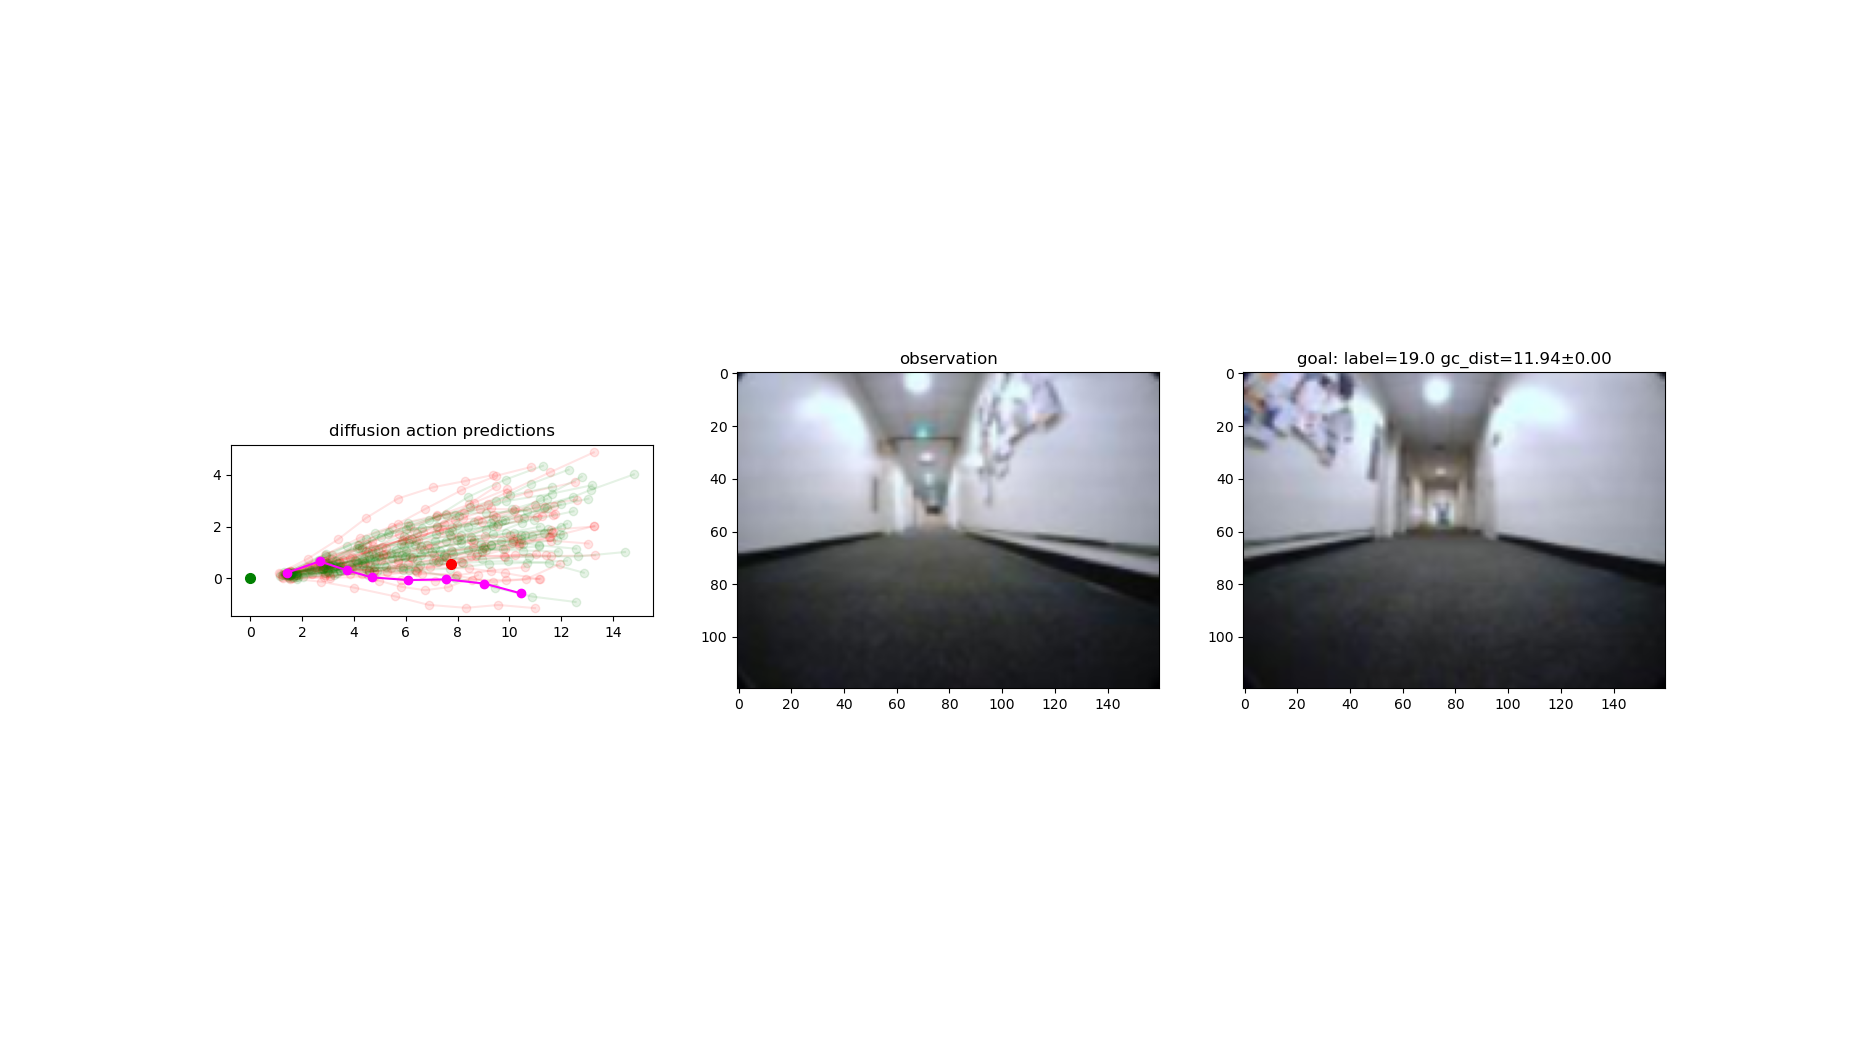
\includegraphics[width=\textwidth]{images/train_action_samples_1.png}    
    \label{fig:train_action_samples_1}
\end{figure}
\begin{figure}[H]
    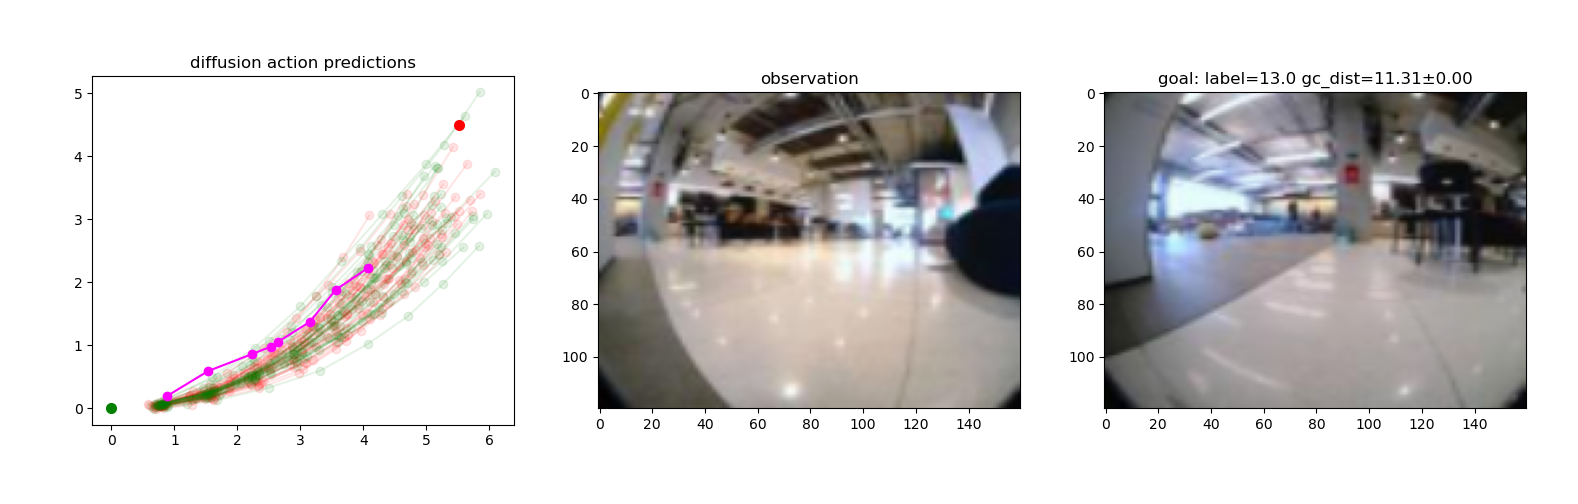
\includegraphics[width=\textwidth]{images/train_action_samples_2.png}
    \label{fig:train_action_samples_1}
\end{figure}
\begin{figure}[H]
    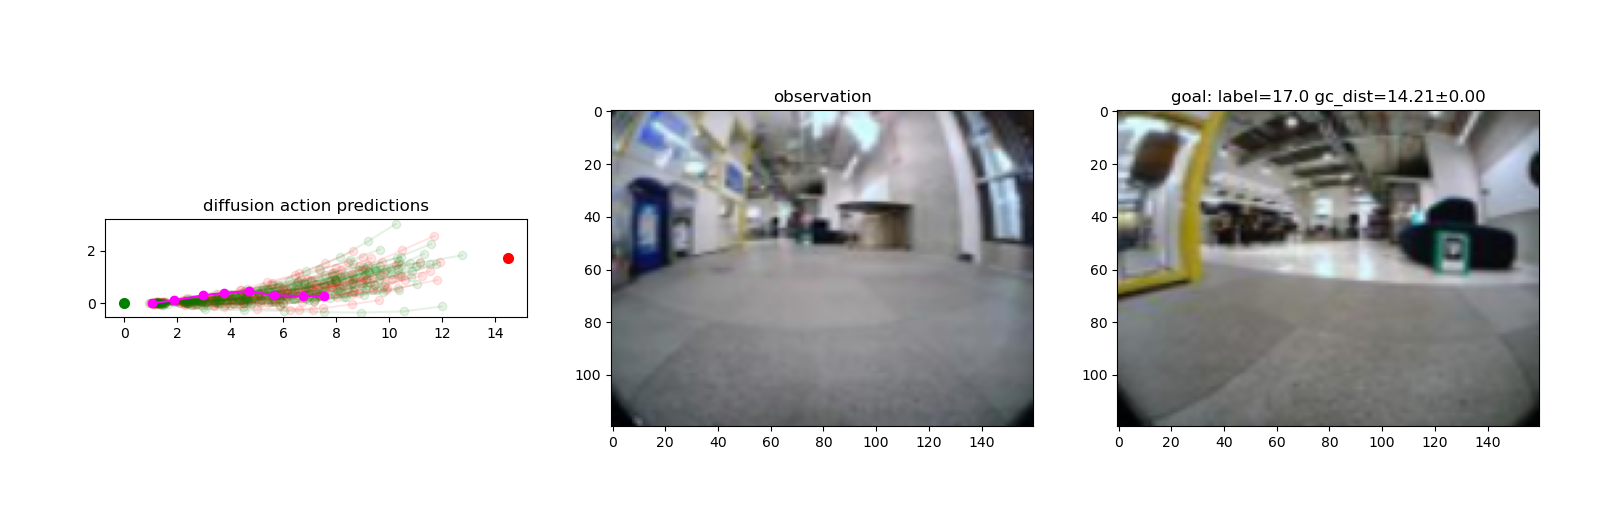
\includegraphics[width=\textwidth]{images/train_action_samples_3.png}
    \label{fig:train_action_samples_1}
\end{figure}
\begin{figure}[H]
    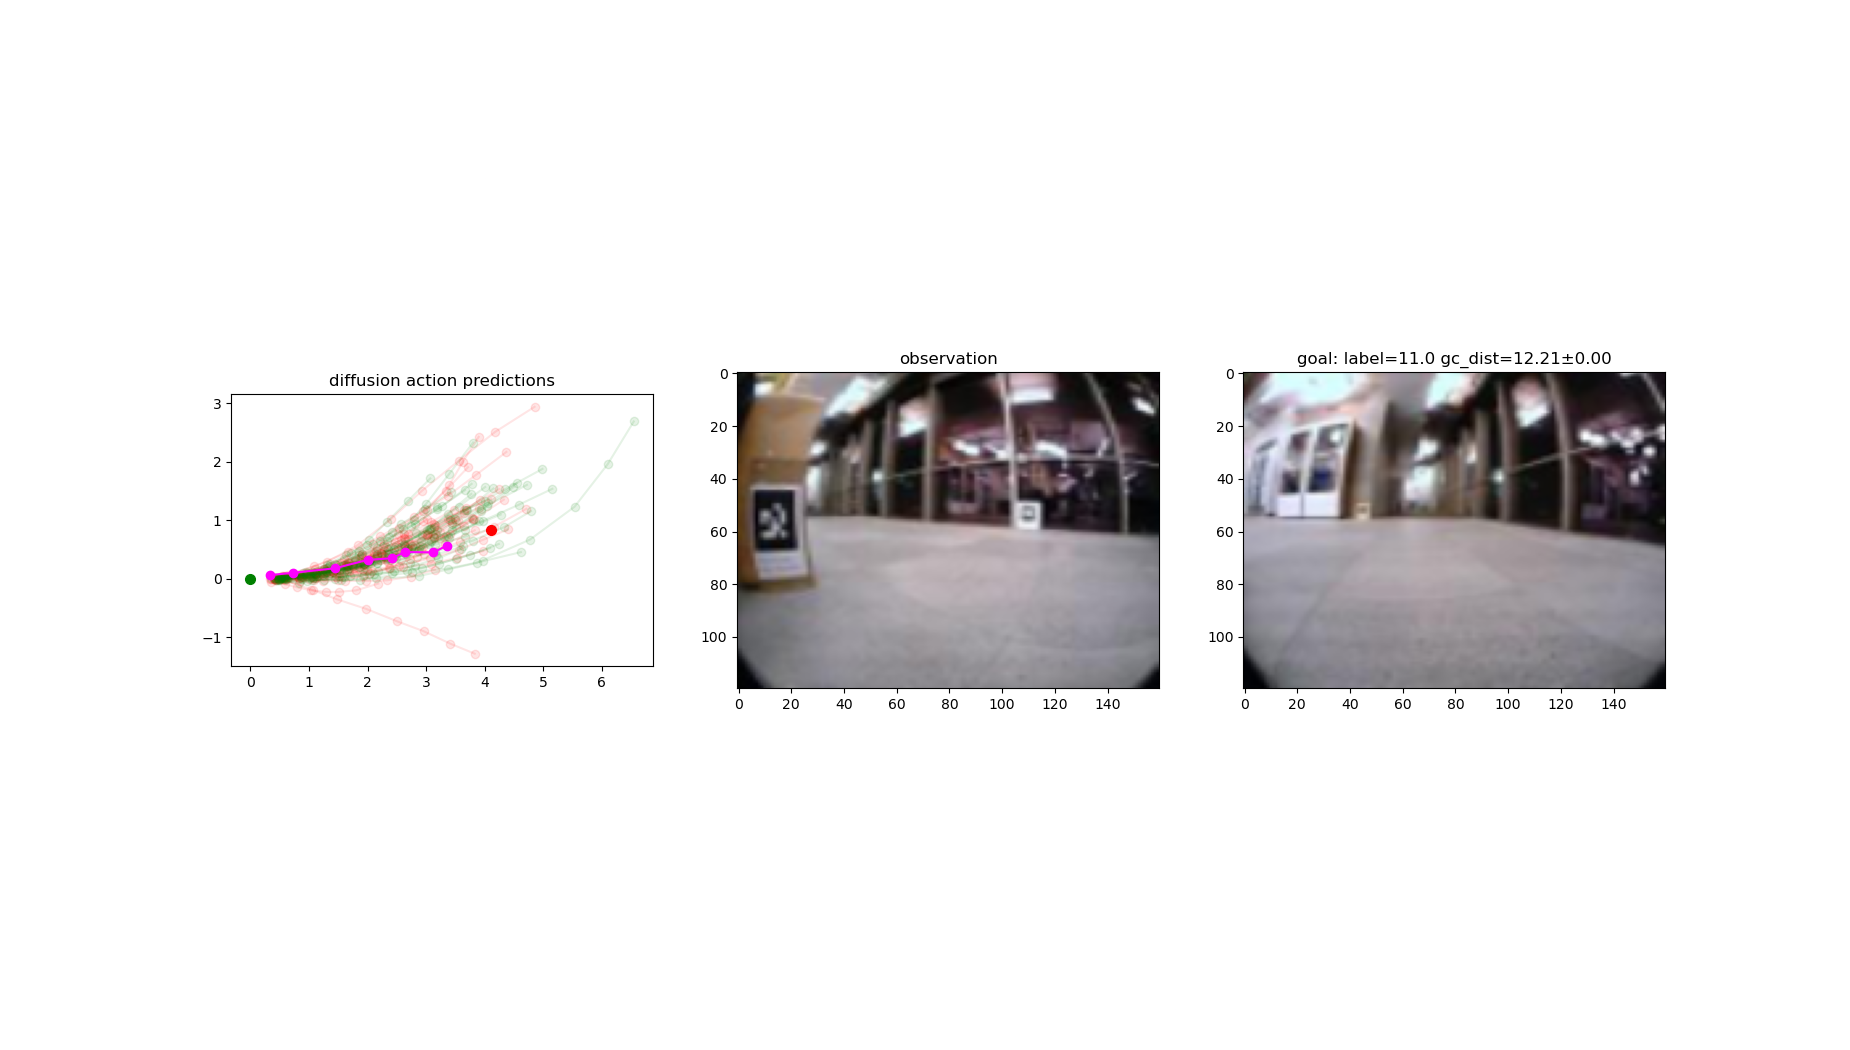
\includegraphics[width=\textwidth]{images/train_action_samples_4.png}
    \label{fig:train_action_samples_1}
\end{figure}
\subsection*{Sacson test action samples:}
\begin{figure}[H]
    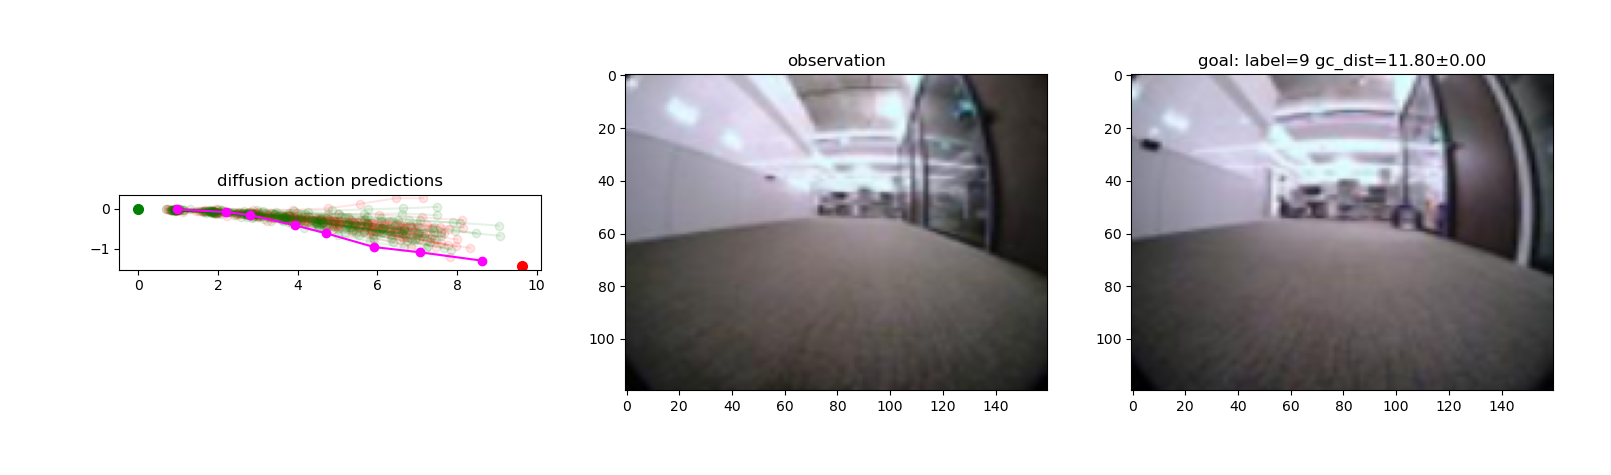
\includegraphics[width=\textwidth]{images/sacson_test_action_samples_1.png}
        \label{fig:sacon_test_action_samples_1}
\end{figure}
\begin{figure}[H]
    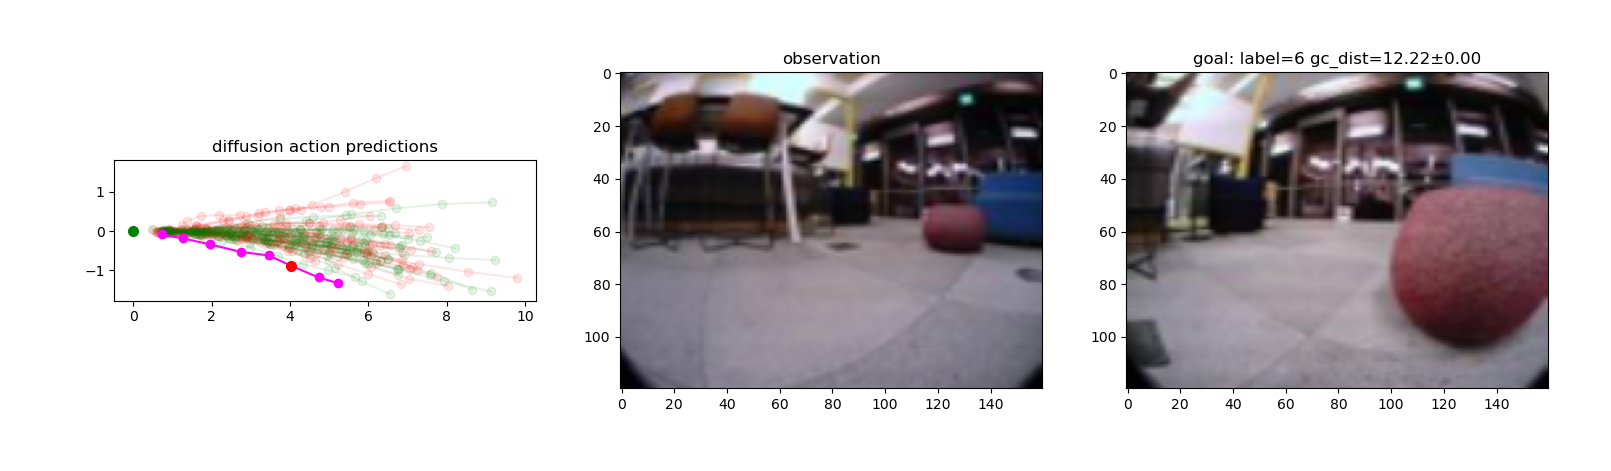
\includegraphics[width=\textwidth]{images/sacson_test_action_samples_2.png}
        \label{fig:sacon_test_action_samples_1}
\end{figure}
\begin{figure}[H]
    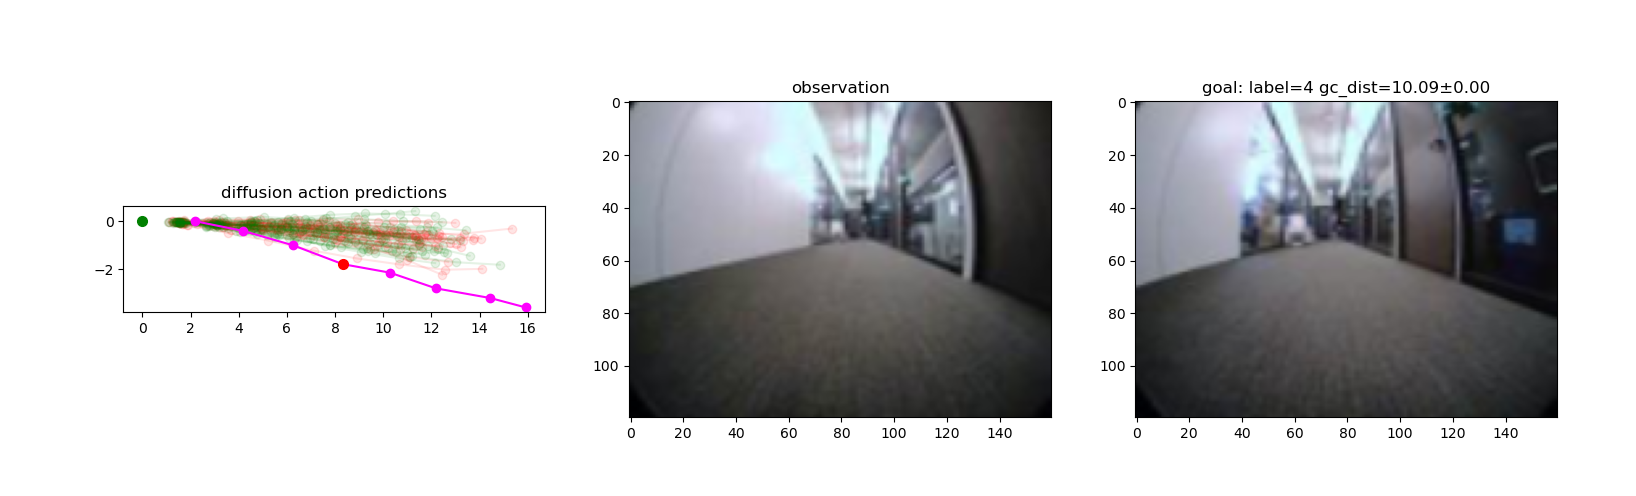
\includegraphics[width=\textwidth]{images/sacson_test_action_samples_3.png}
        \label{fig:sacon_test_action_samples_1}
\end{figure}


\subsection*{Goal-Conditioned (GC) Evaluation}
We set the goal mask $m = 0$ to evaluate the model's performance in goal-directed navigation.\\
\noindent \textbf{Distance Loss:}\\
\begin{figure}[H]
    \centering
    \begin{subfigure}[b]{0.48\textwidth}
        \centering
        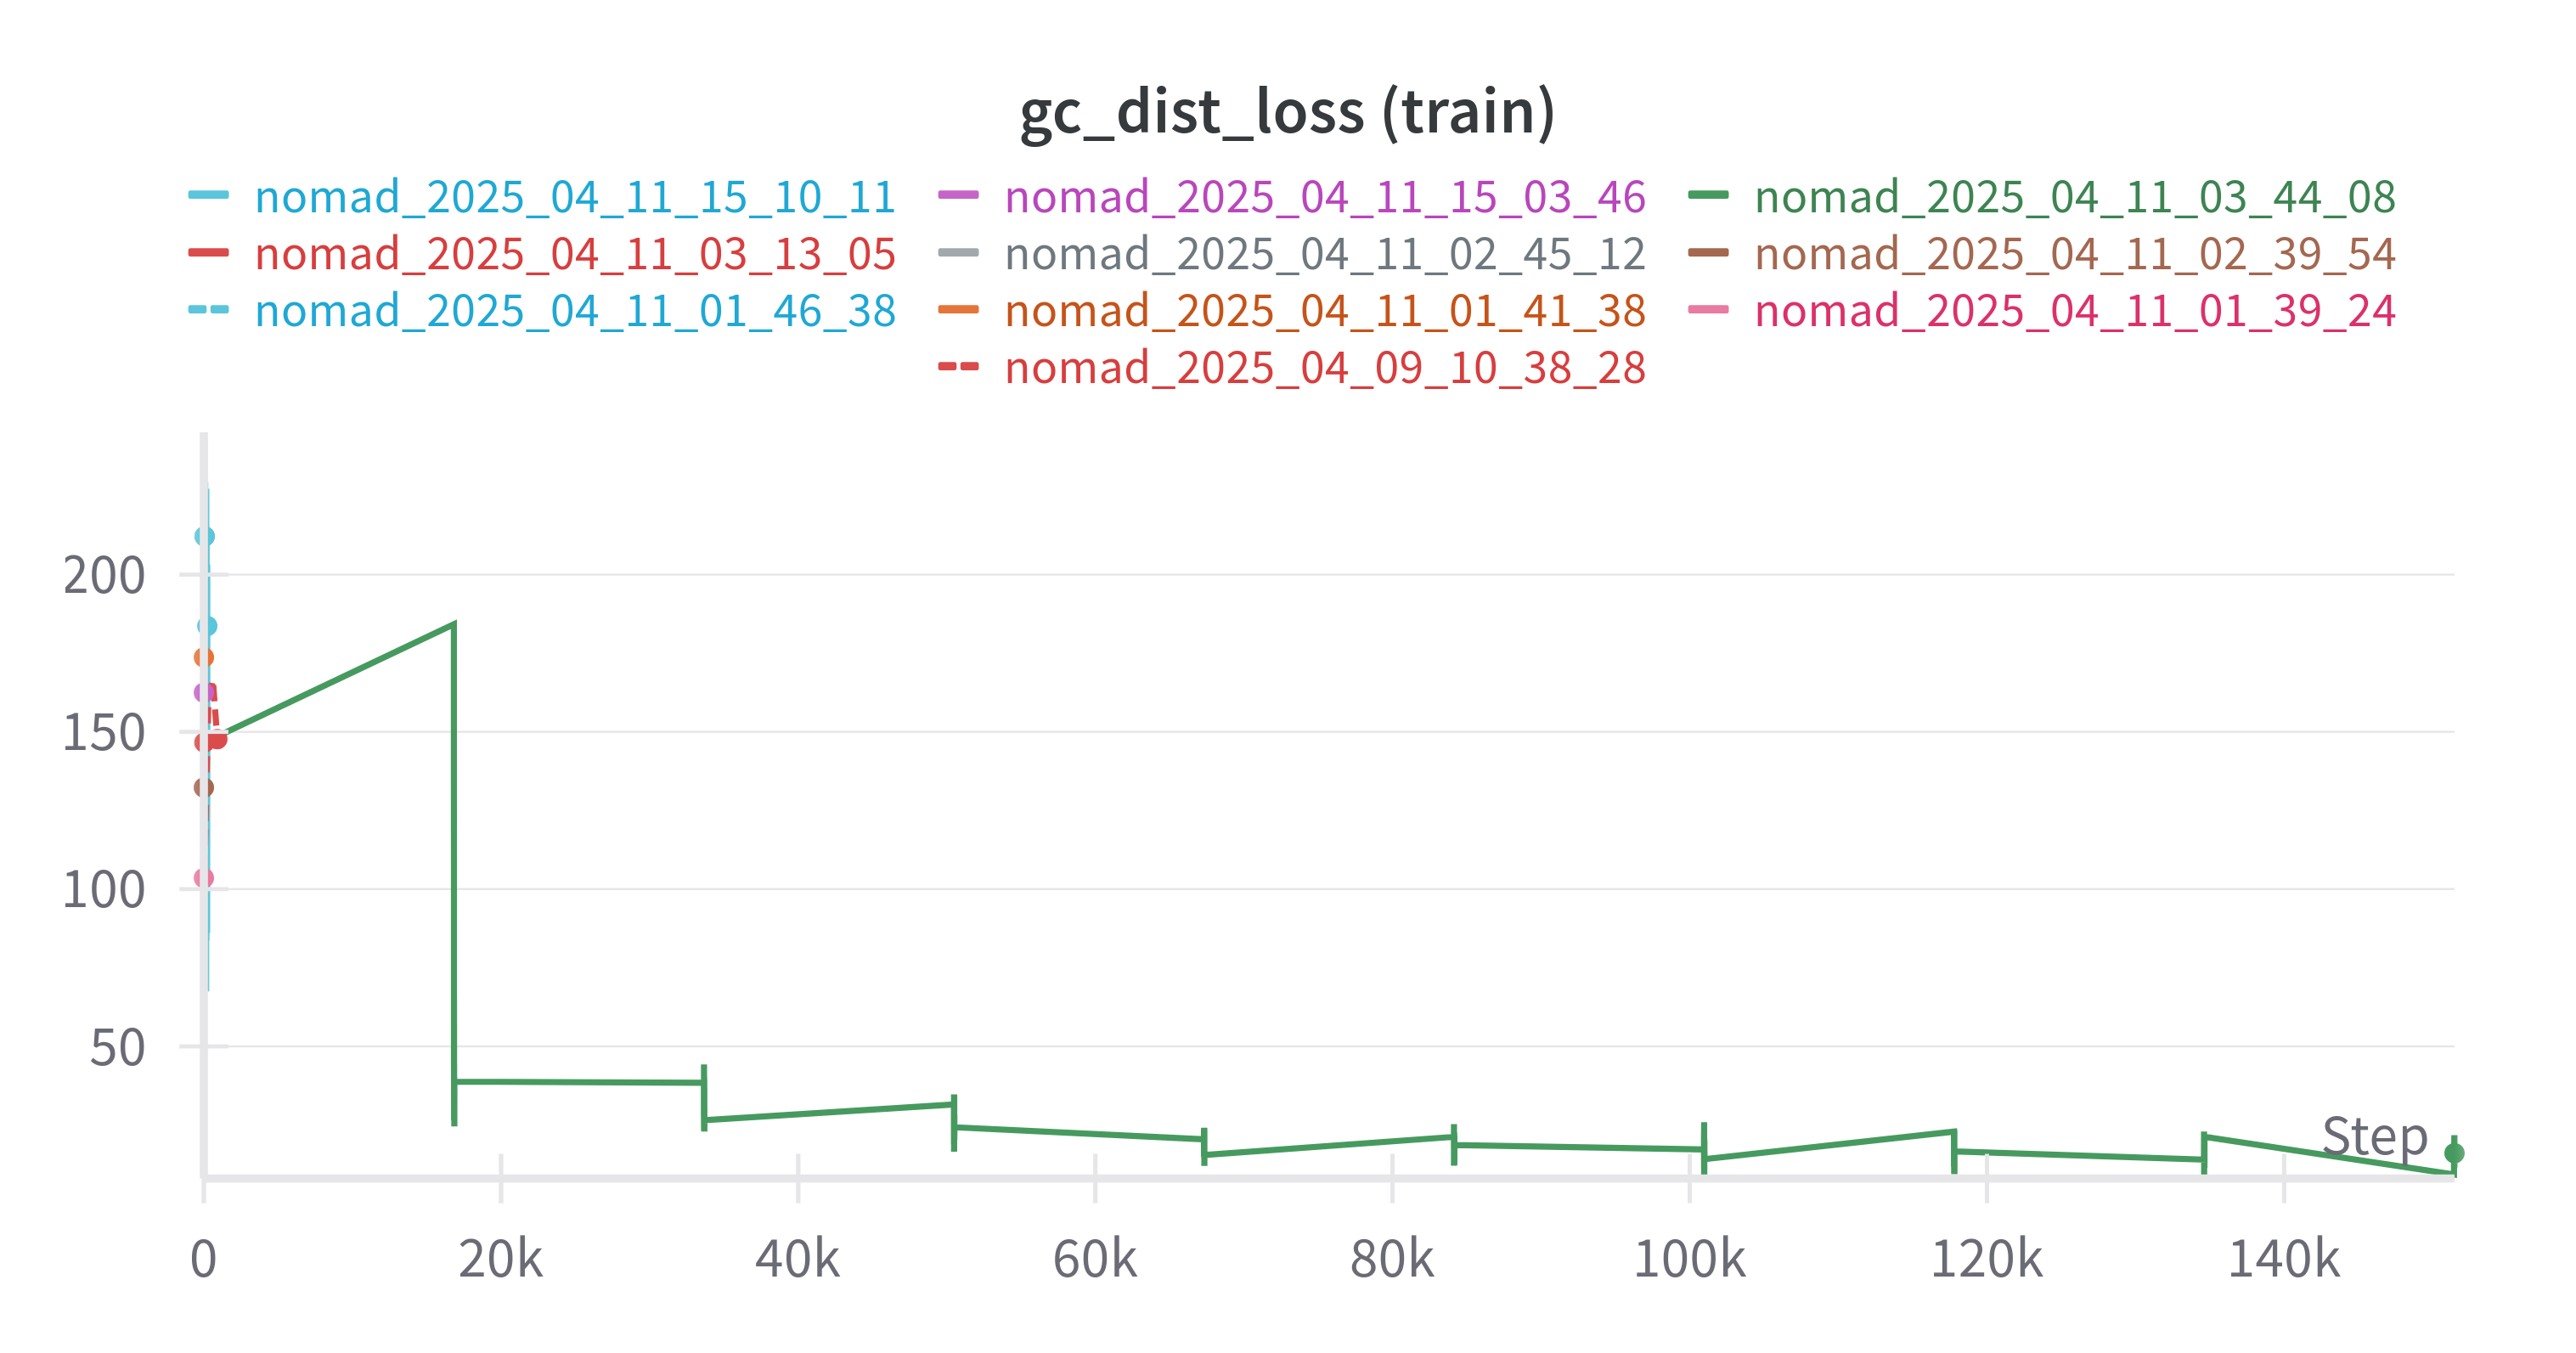
\includegraphics[width=\textwidth]{images/gc_distloss_nomad.png}
        \caption{Distance Loss on Training Set}
        \label{fig:gc_dist_loss_train}
    \end{subfigure}
    \hfill
    \begin{subfigure}[b]{0.48\textwidth}
        \centering
        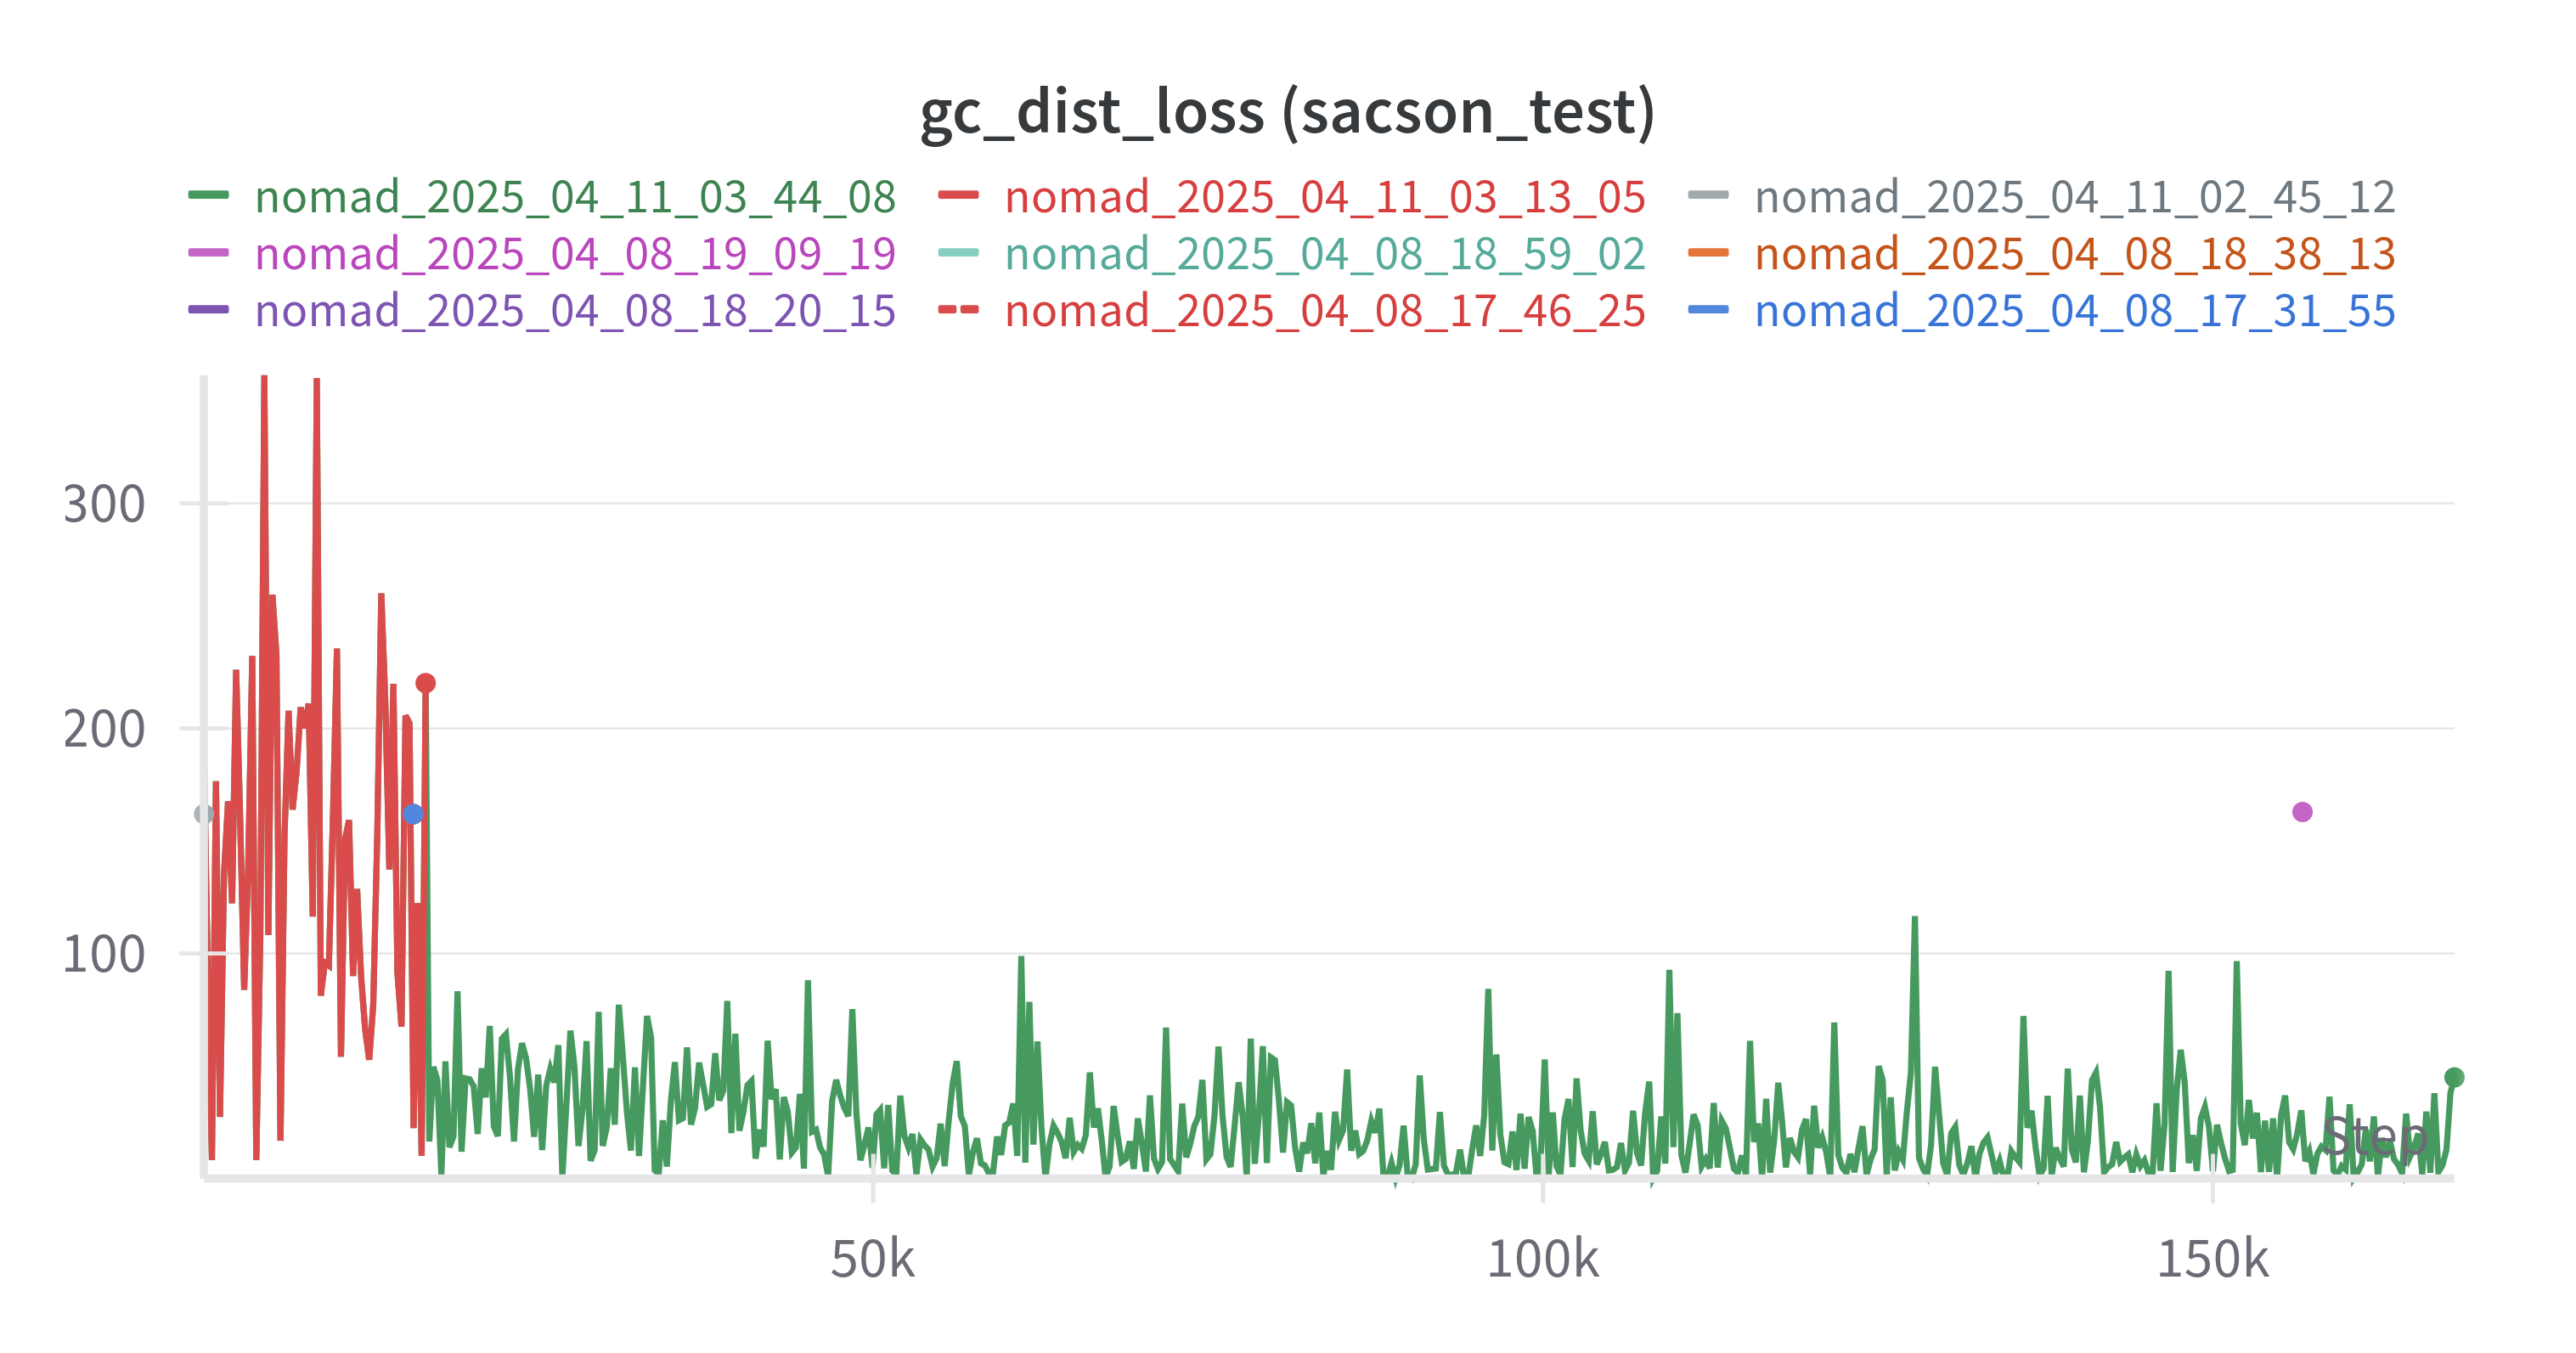
\includegraphics[width=\textwidth]{images/gc_dist_loss_test.png}
        \caption{Distance Loss on Validation Set}
        \label{fig:gc_dist_loss_val}
    \end{subfigure}
    \caption{Distance loss comparison between training and validation sets under goal-conditioned evaluation.}
\end{figure}
We see that the loss has plateaued after the first epoch, both in test and training sets, indicating that the model quickly learns a strong initial estimate of the distance to the goal.\\

\noindent \textbf{Action loss:}\\
\begin{figure}[H]
    \centering
    \begin{subfigure}[b]{0.48\textwidth}
        \centering
        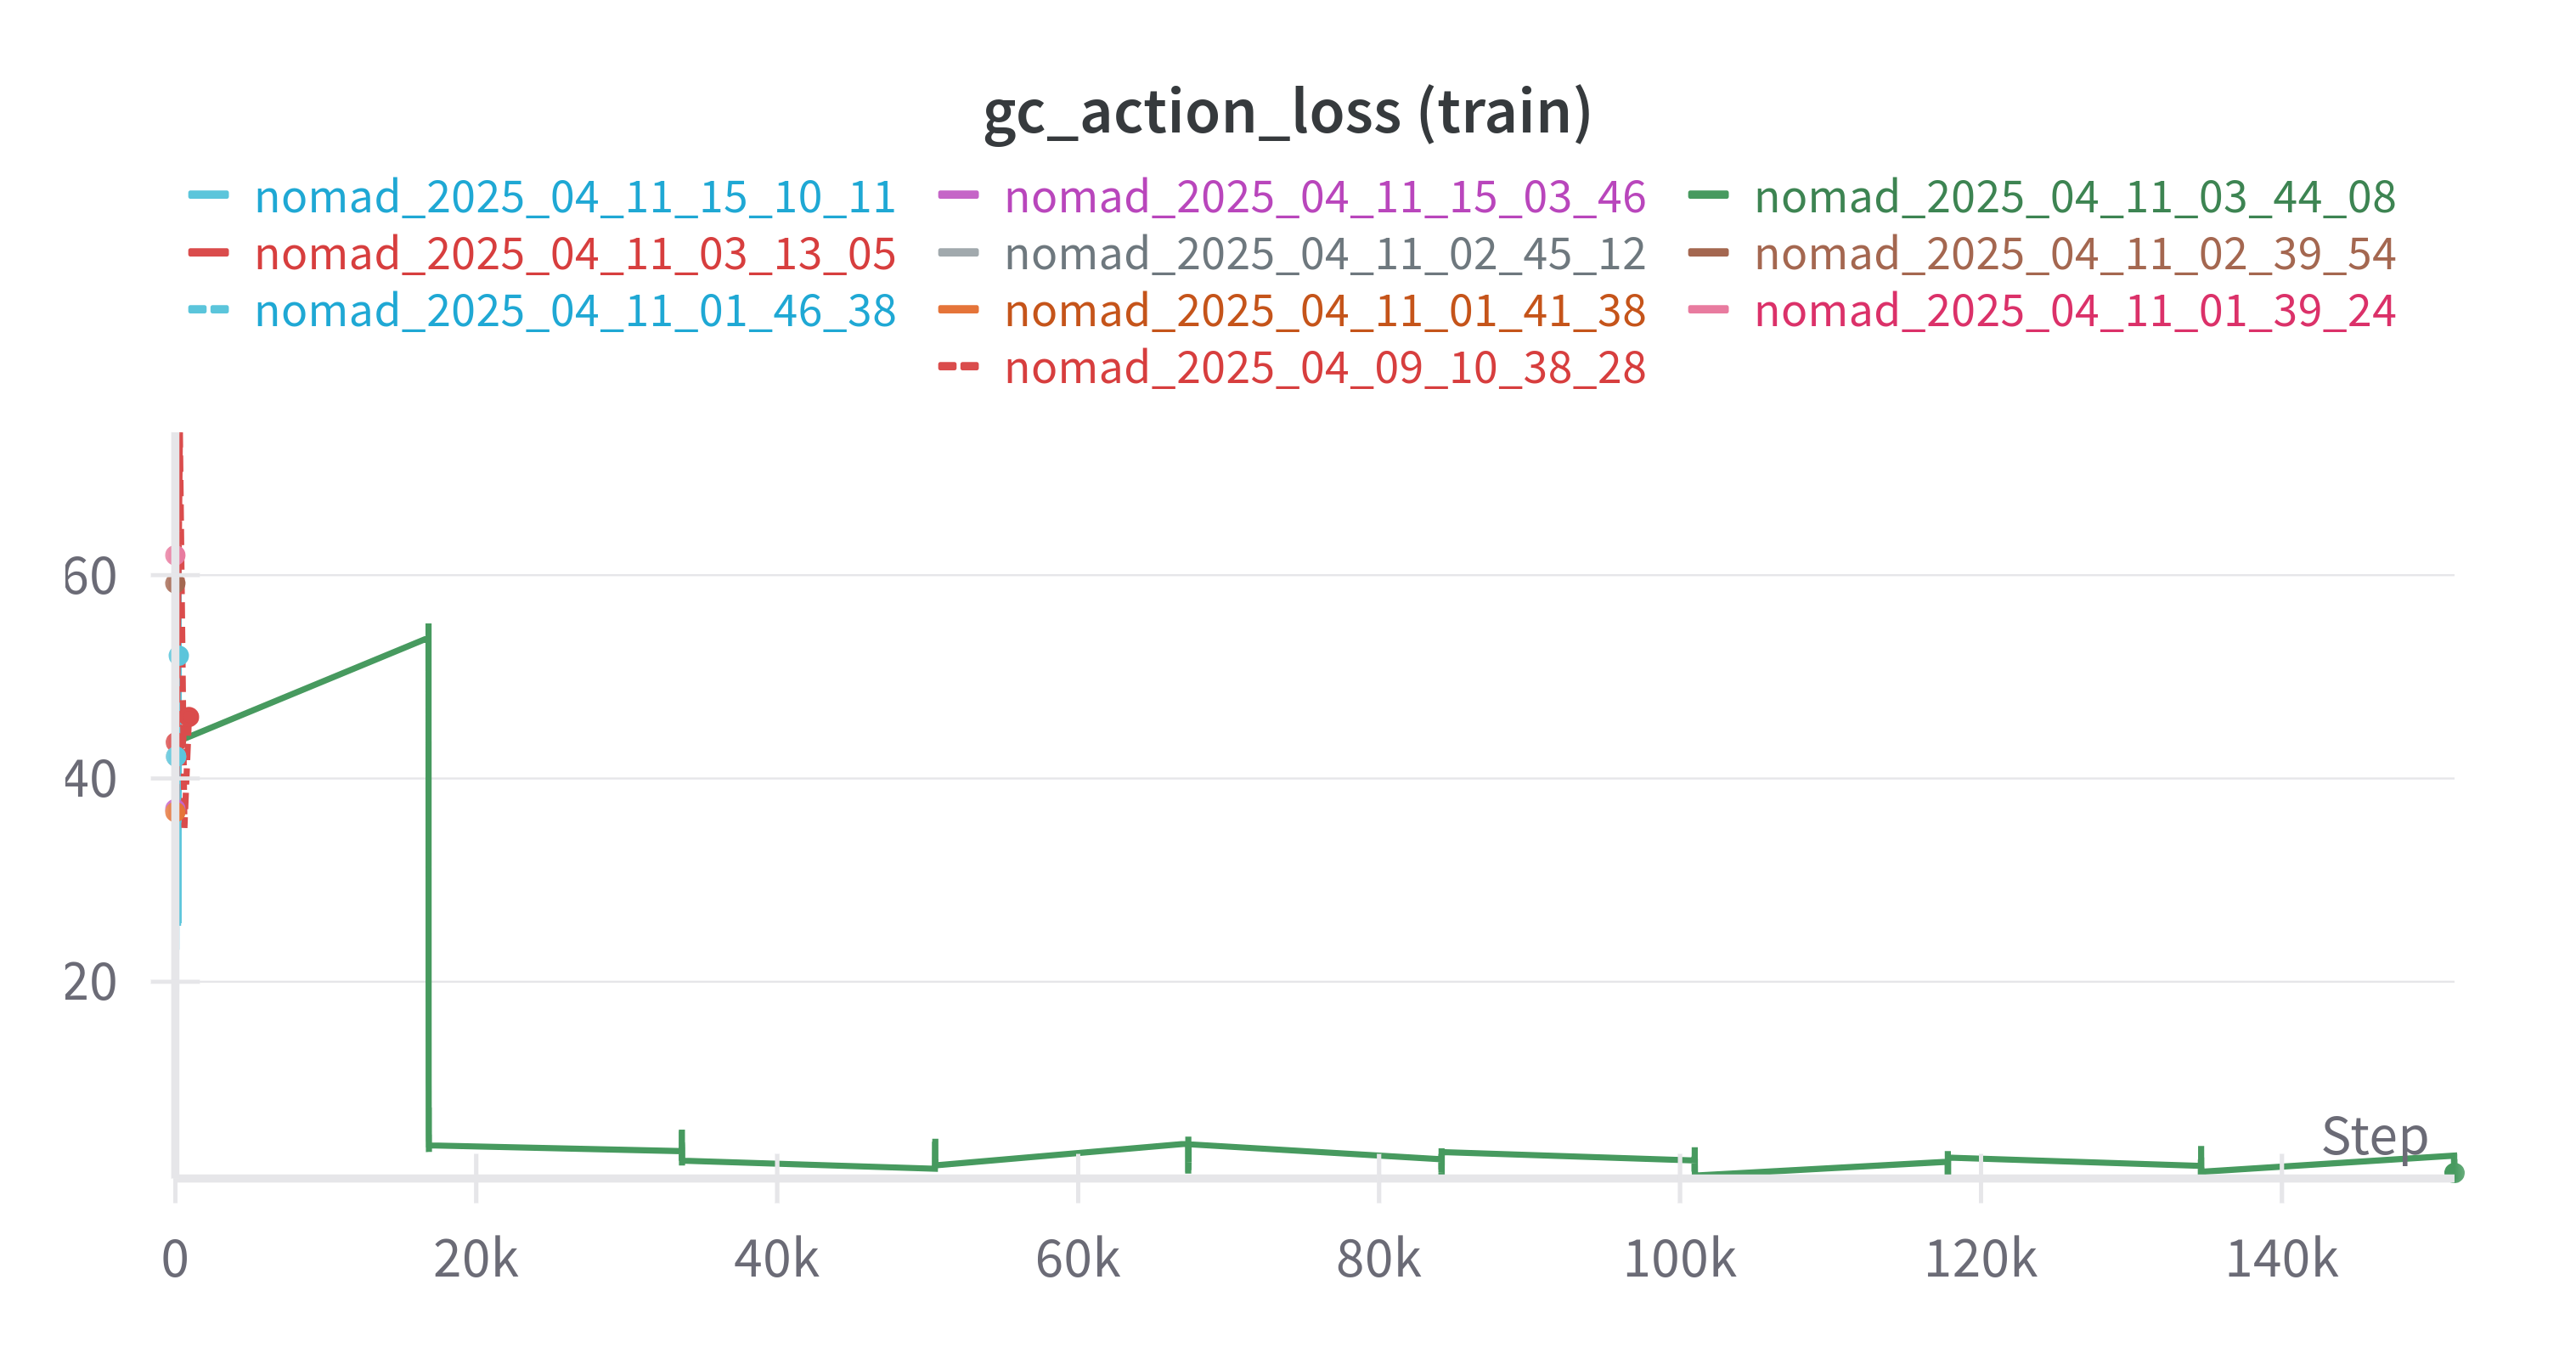
\includegraphics[width=\textwidth]{images/gc_actionloss_nomad.png}
        \caption{Action Loss on Training Set}
        \label{fig:gc_action_loss_train}
    \end{subfigure}
    \hfill
    \begin{subfigure}[b]{0.48\textwidth}
        \centering
        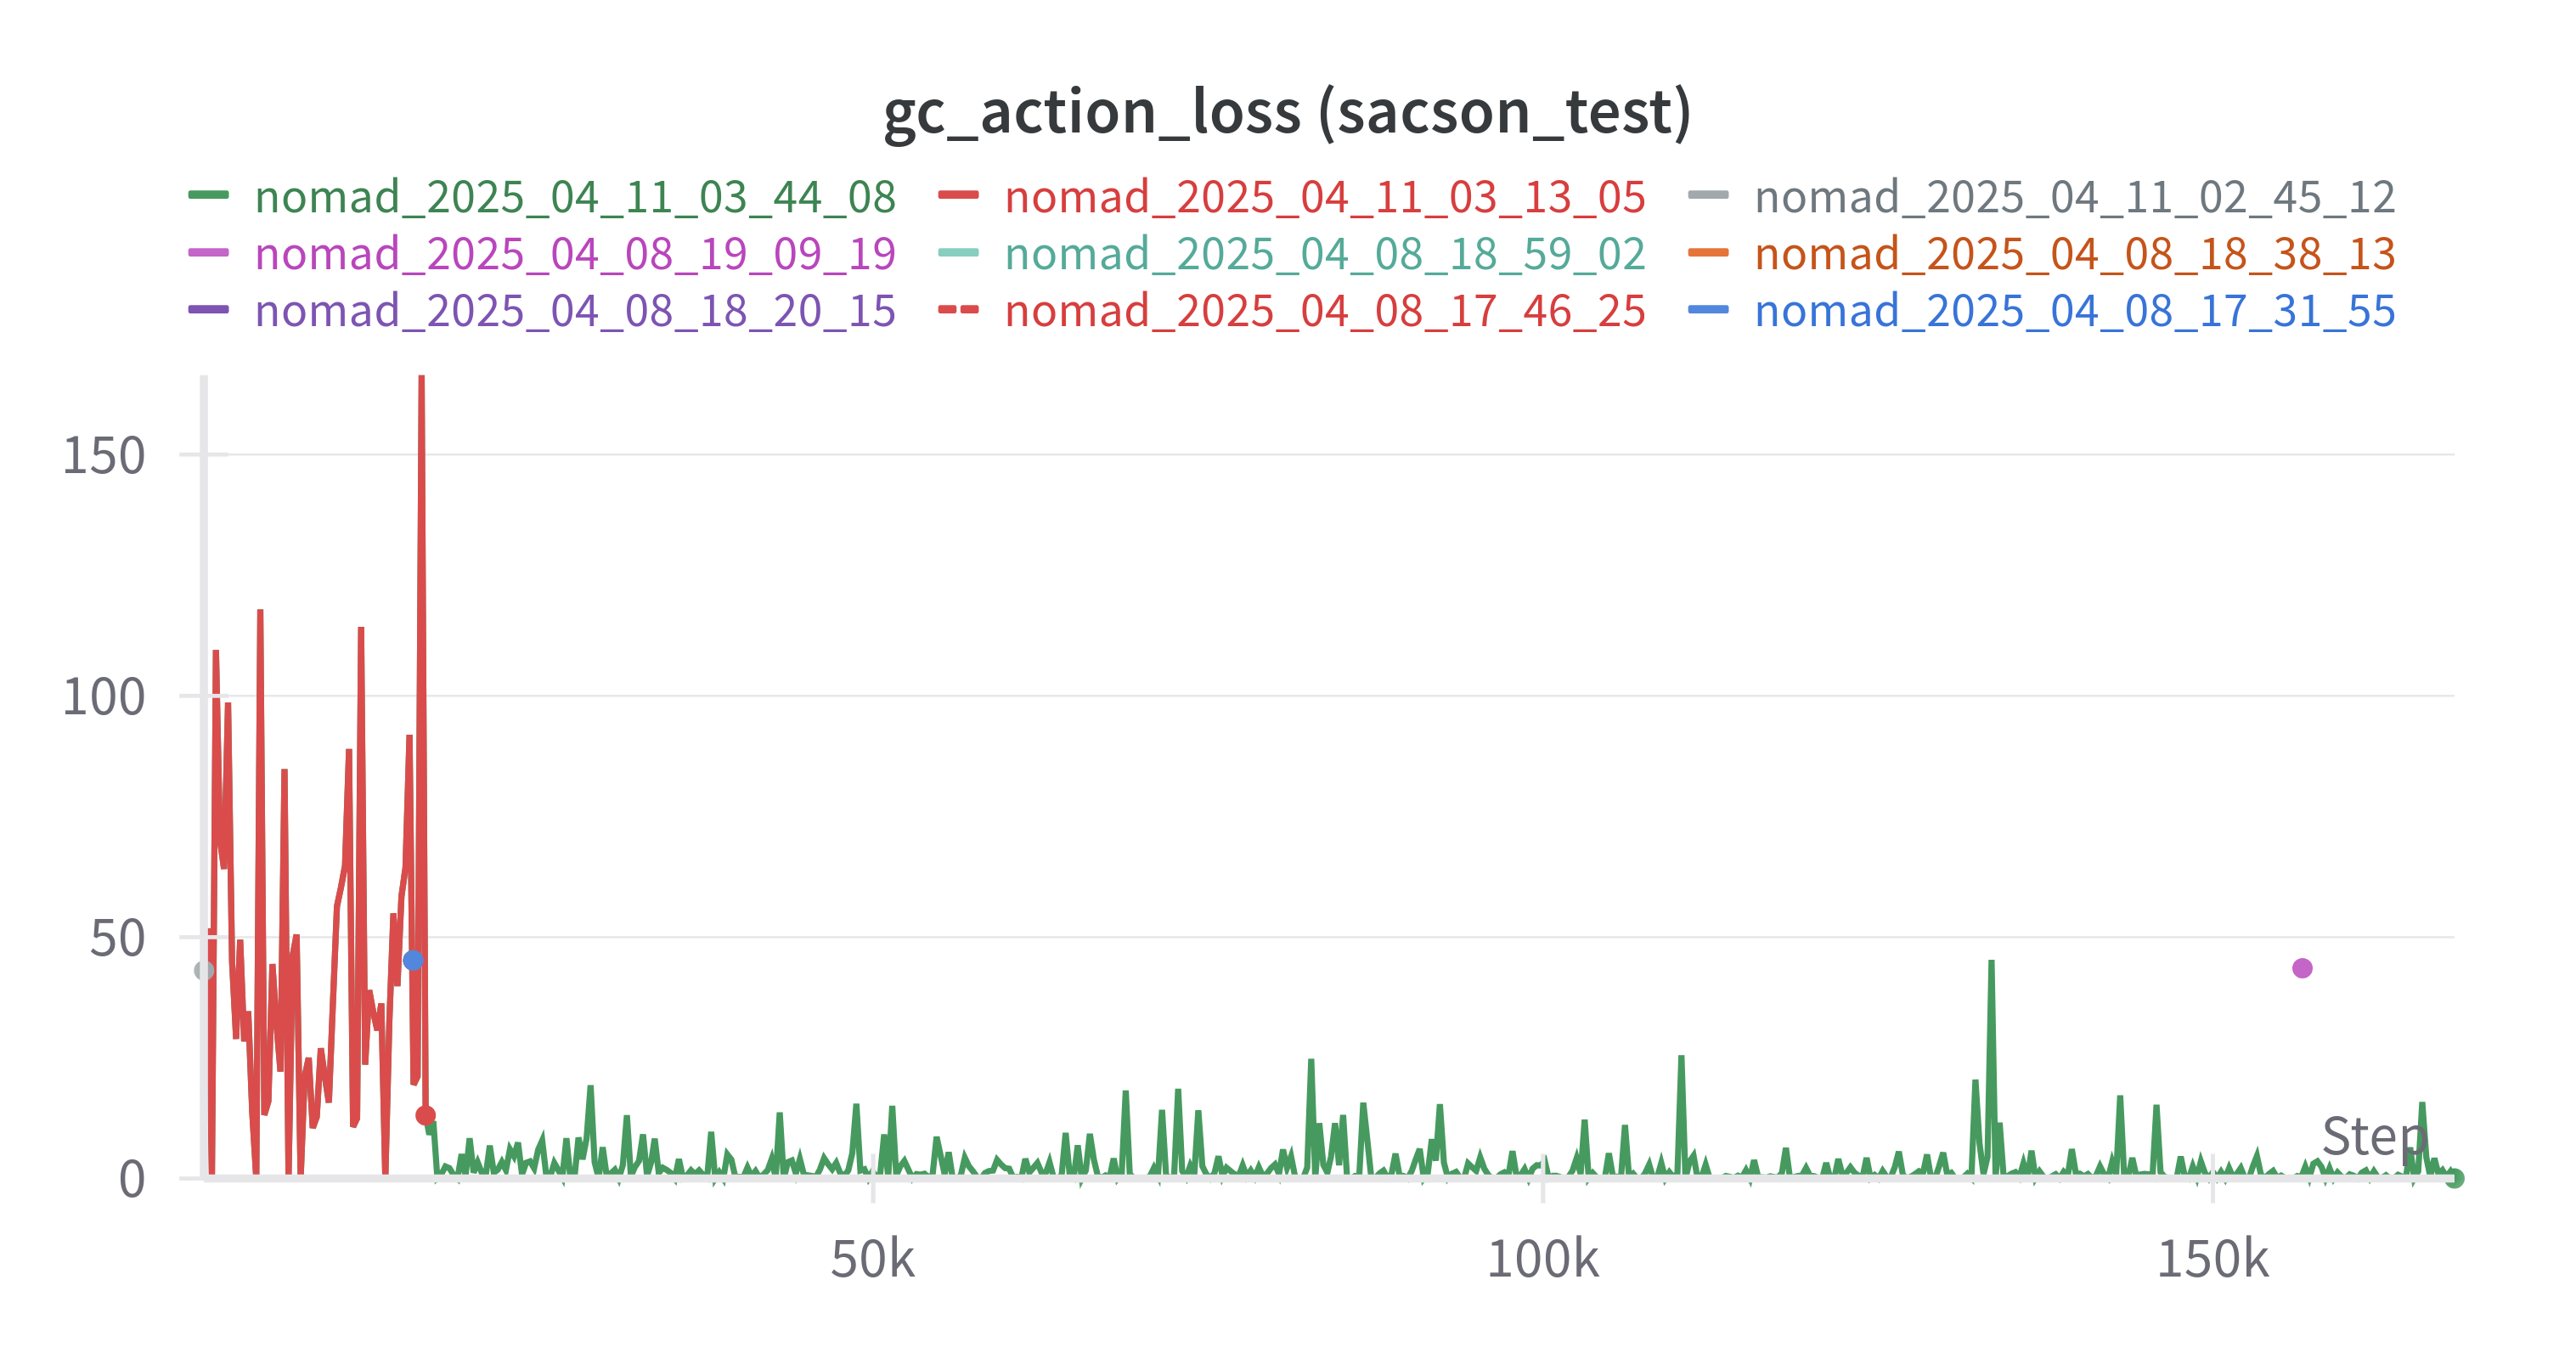
\includegraphics[width=\textwidth]{images/gc_actionloss_test_nomad.png}
        \caption{Action Loss on Validation Set}
        \label{fig:gc_action_loss_val}
    \end{subfigure}
    \caption{Action loss comparison between training and validation sets under goal-conditioned evaluation.}
\end{figure}
The action loss steadily decreases across epochs in both training and validation datasets, suggesting that the diffusion-based policy learns to generate feasible future actions conditioned on the visual goal and current context.\\

\noindent \textbf{gc\_action\_waypts\_cos\_sim:}\\
\begin{figure}[H]
    \centering
    \begin{subfigure}[b]{0.48\textwidth}
        \centering
        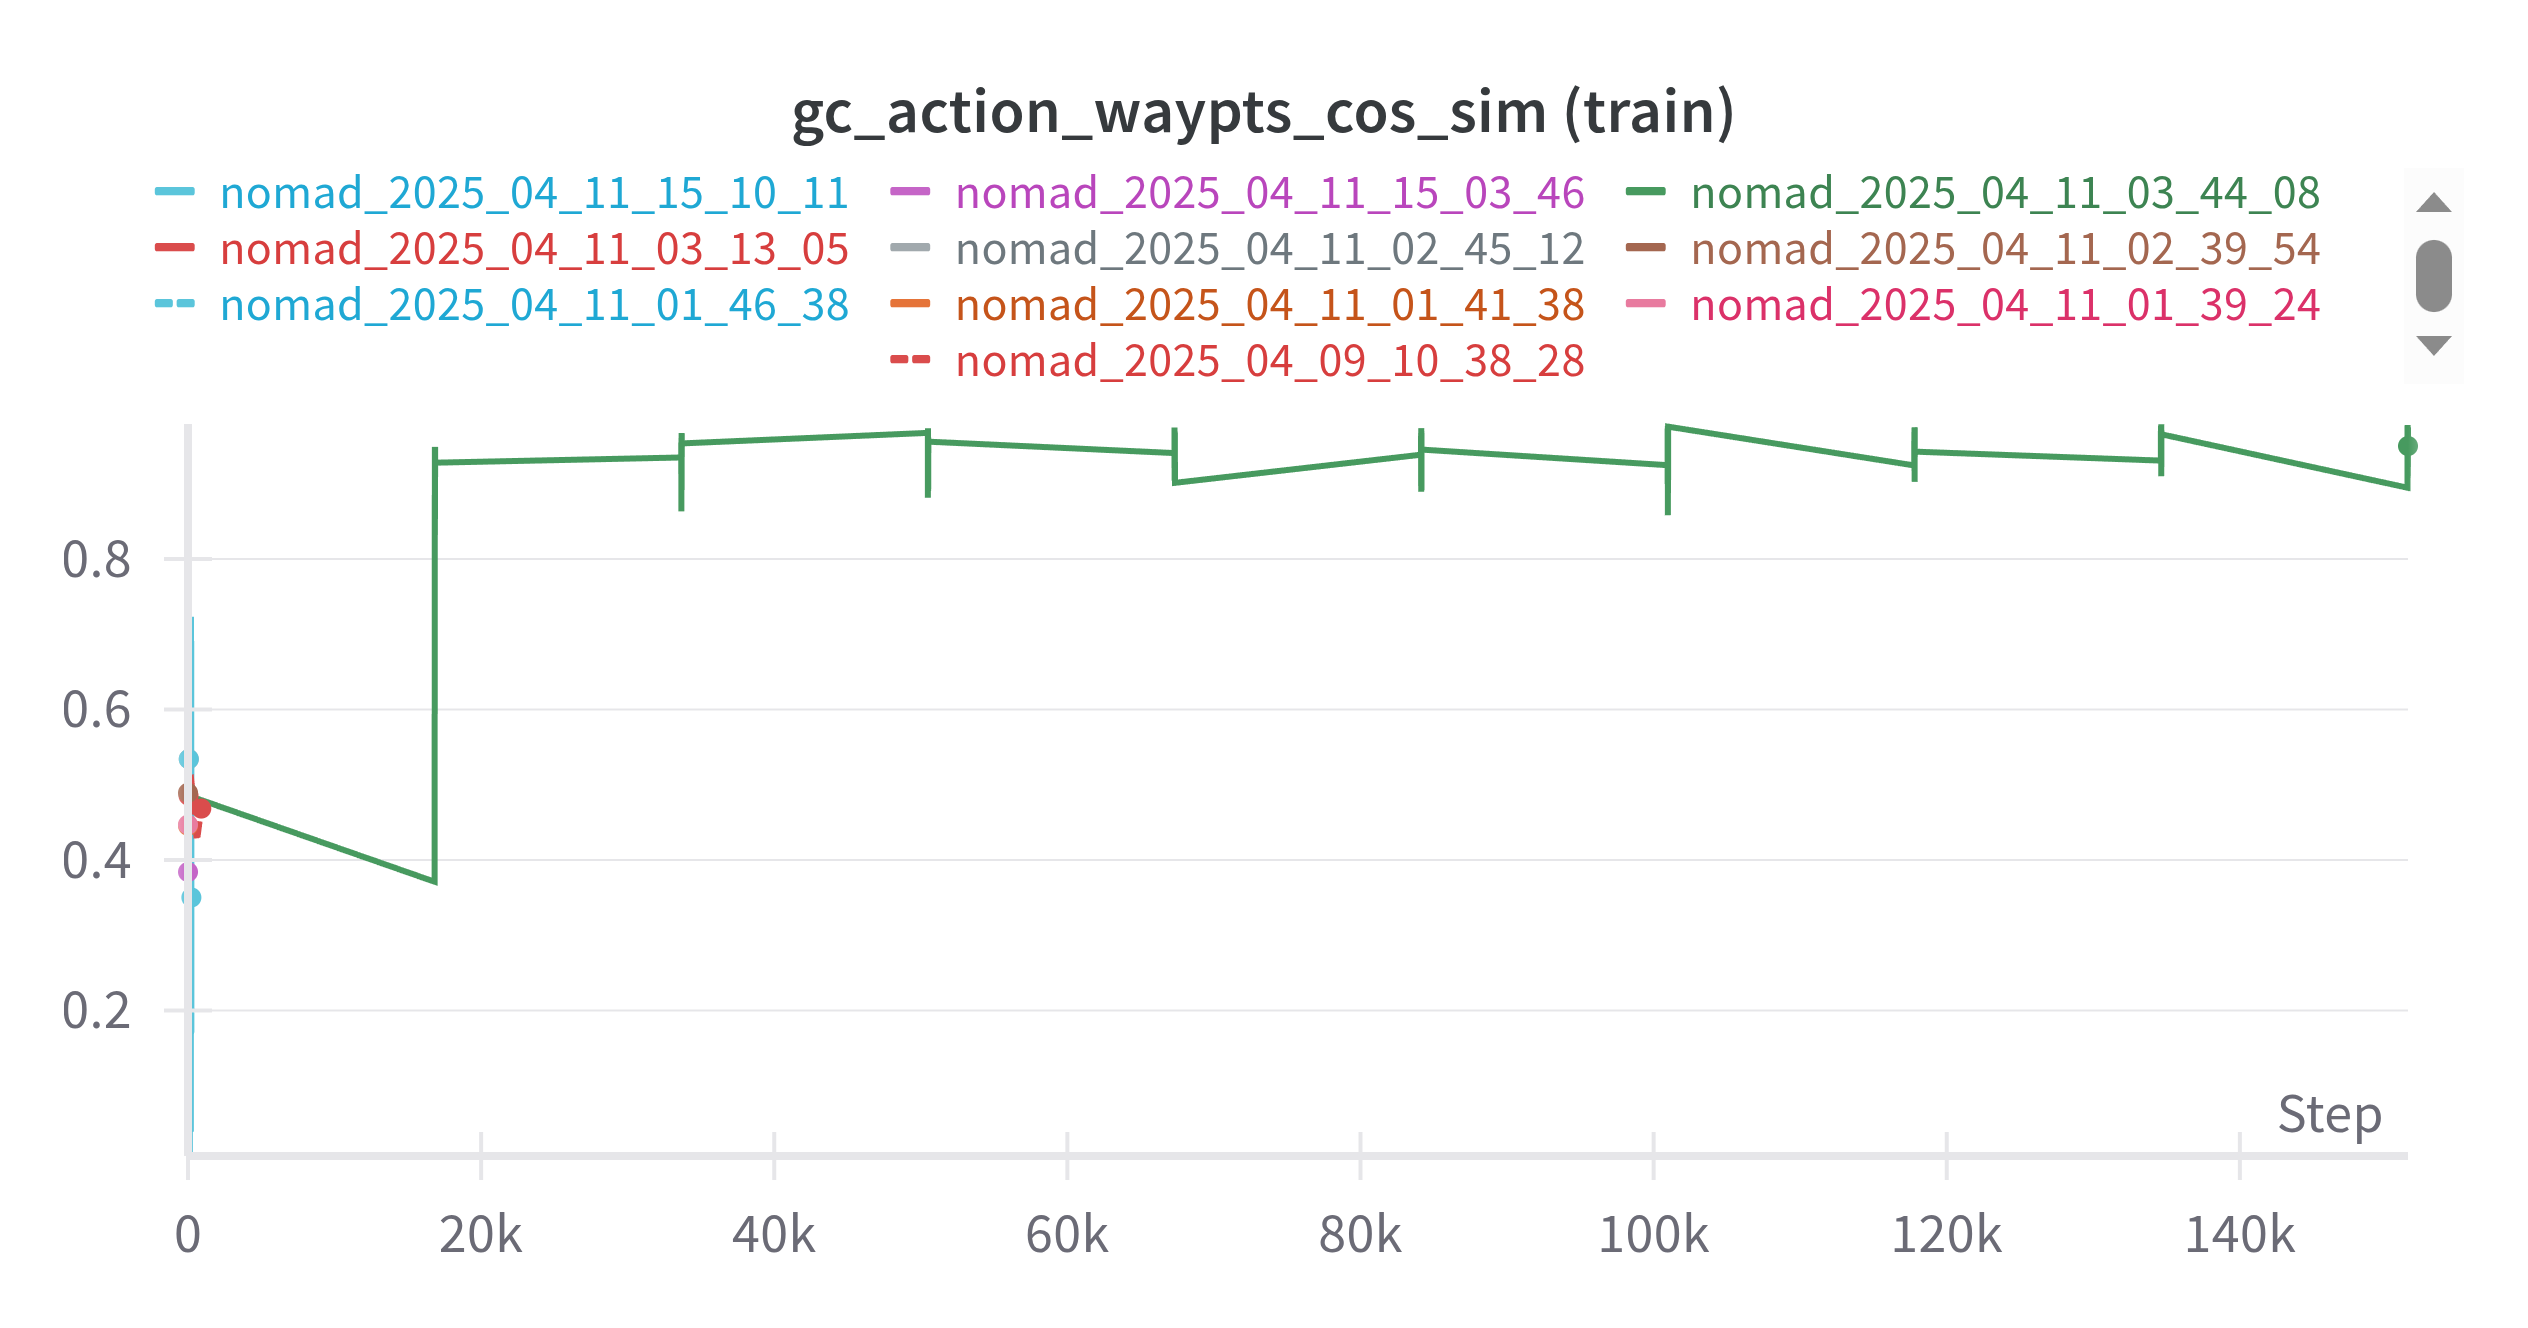
\includegraphics[width=\textwidth]{images/gc_action_waypts_cos_sim_train.png}
        \caption{Cosine Similarity on Training Set}
        \label{fig:gc_action_waypts_cos_sim_train}
    \end{subfigure}
    \hfill
    \begin{subfigure}[b]{0.48\textwidth}
        \centering
        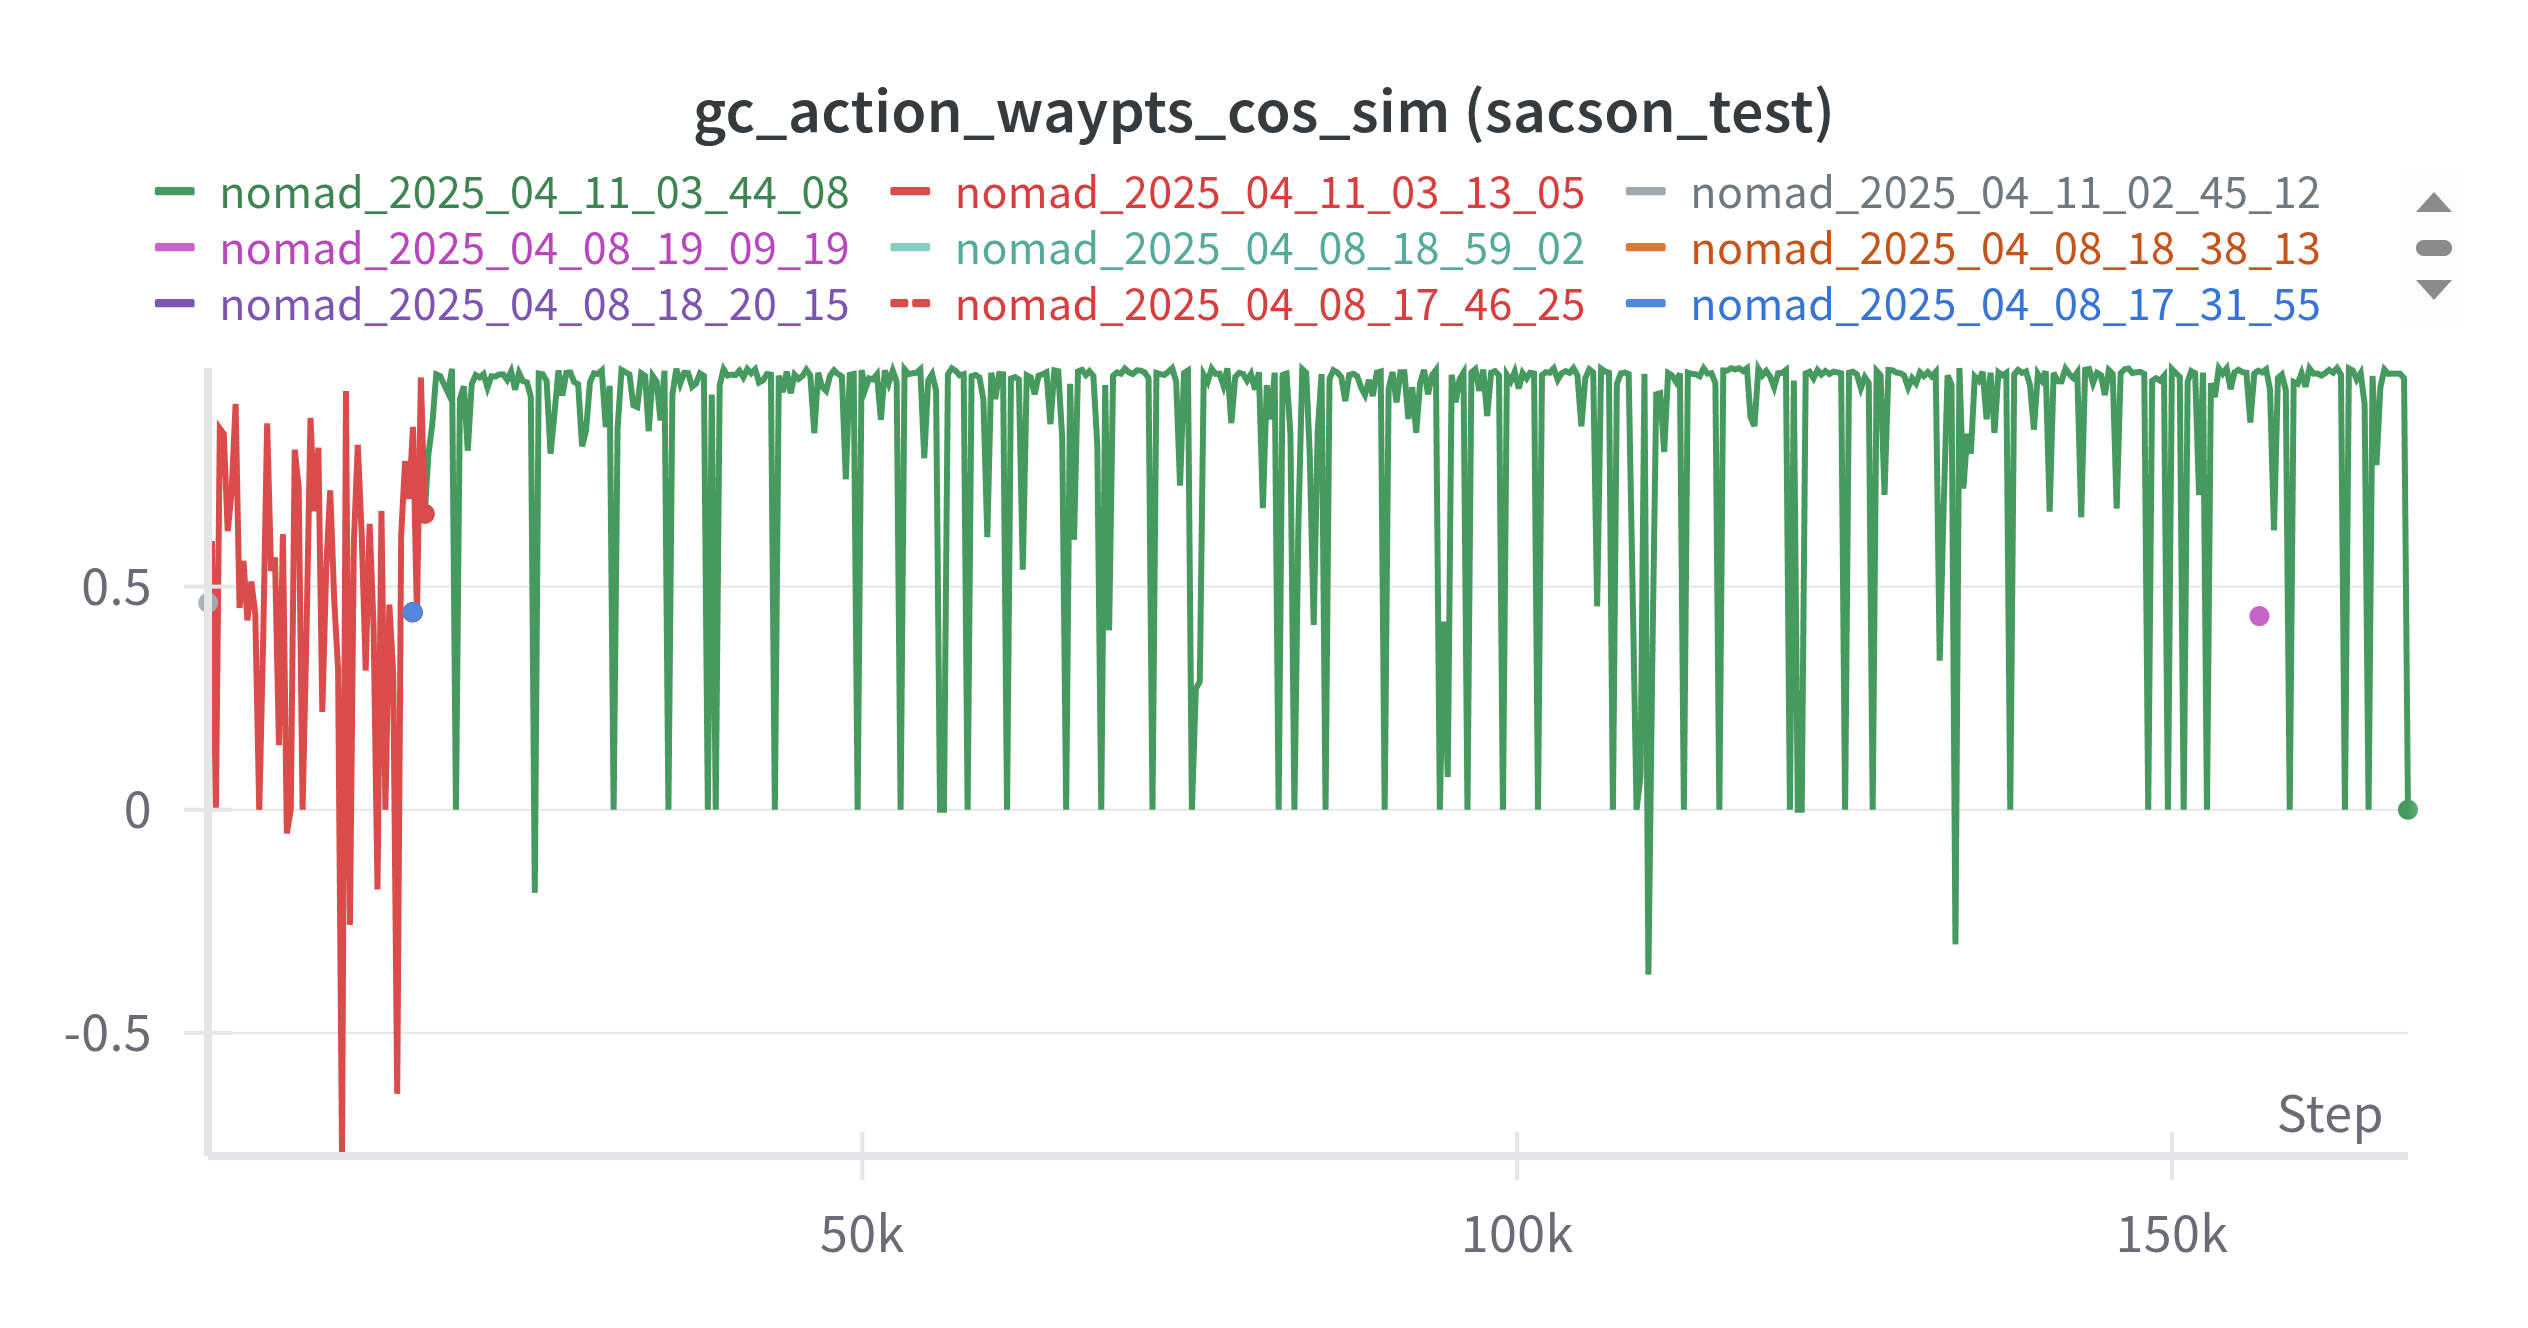
\includegraphics[width=\textwidth]{images/gc_action_waypts_cos_sim_test.png}
        \caption{Cosine Similarity on Validation Set}
        \label{fig:gc_action_waypts_cos_sim_val}
    \end{subfigure}
    \caption{Cosine similarity between predicted and ground-truth waypoints on the training and validation sets under goal-conditioned evaluation.}
\end{figure}
The Cosine Similarity metric evaluates how well the predicted action direction aligns with the ground-truth direction by measuring the angle between the two vectors. A value closer to 1 indicates better directional alignment.

\begin{itemize}
    \item During training, the model achieves a high and stable cosine similarity on the training set, indicating that it effectively learns to predict actions aligned with the ground-truth directions in seen environments.
    \item However, the validation set shows noticeable variance in cosine similarity across epochs. This could be attributed to the fact that the dataset configuration had \texttt{learn\_angle = False}, meaning the model was not explicitly trained to predict the robot's orientation or angular displacement.
    \item As a result, while the model can align its predictions in direction (to some extent), the lack of angular supervision might reduce its generalization capacity in unseen environments, leading to inconsistency in cosine similarity.
\end{itemize}
\noindent \textbf{gc\_multi\_action\_waypts\_cos\_sim:}\\
\begin{figure}[H]
    \centering
    \begin{subfigure}[b]{0.48\textwidth}
        \centering
        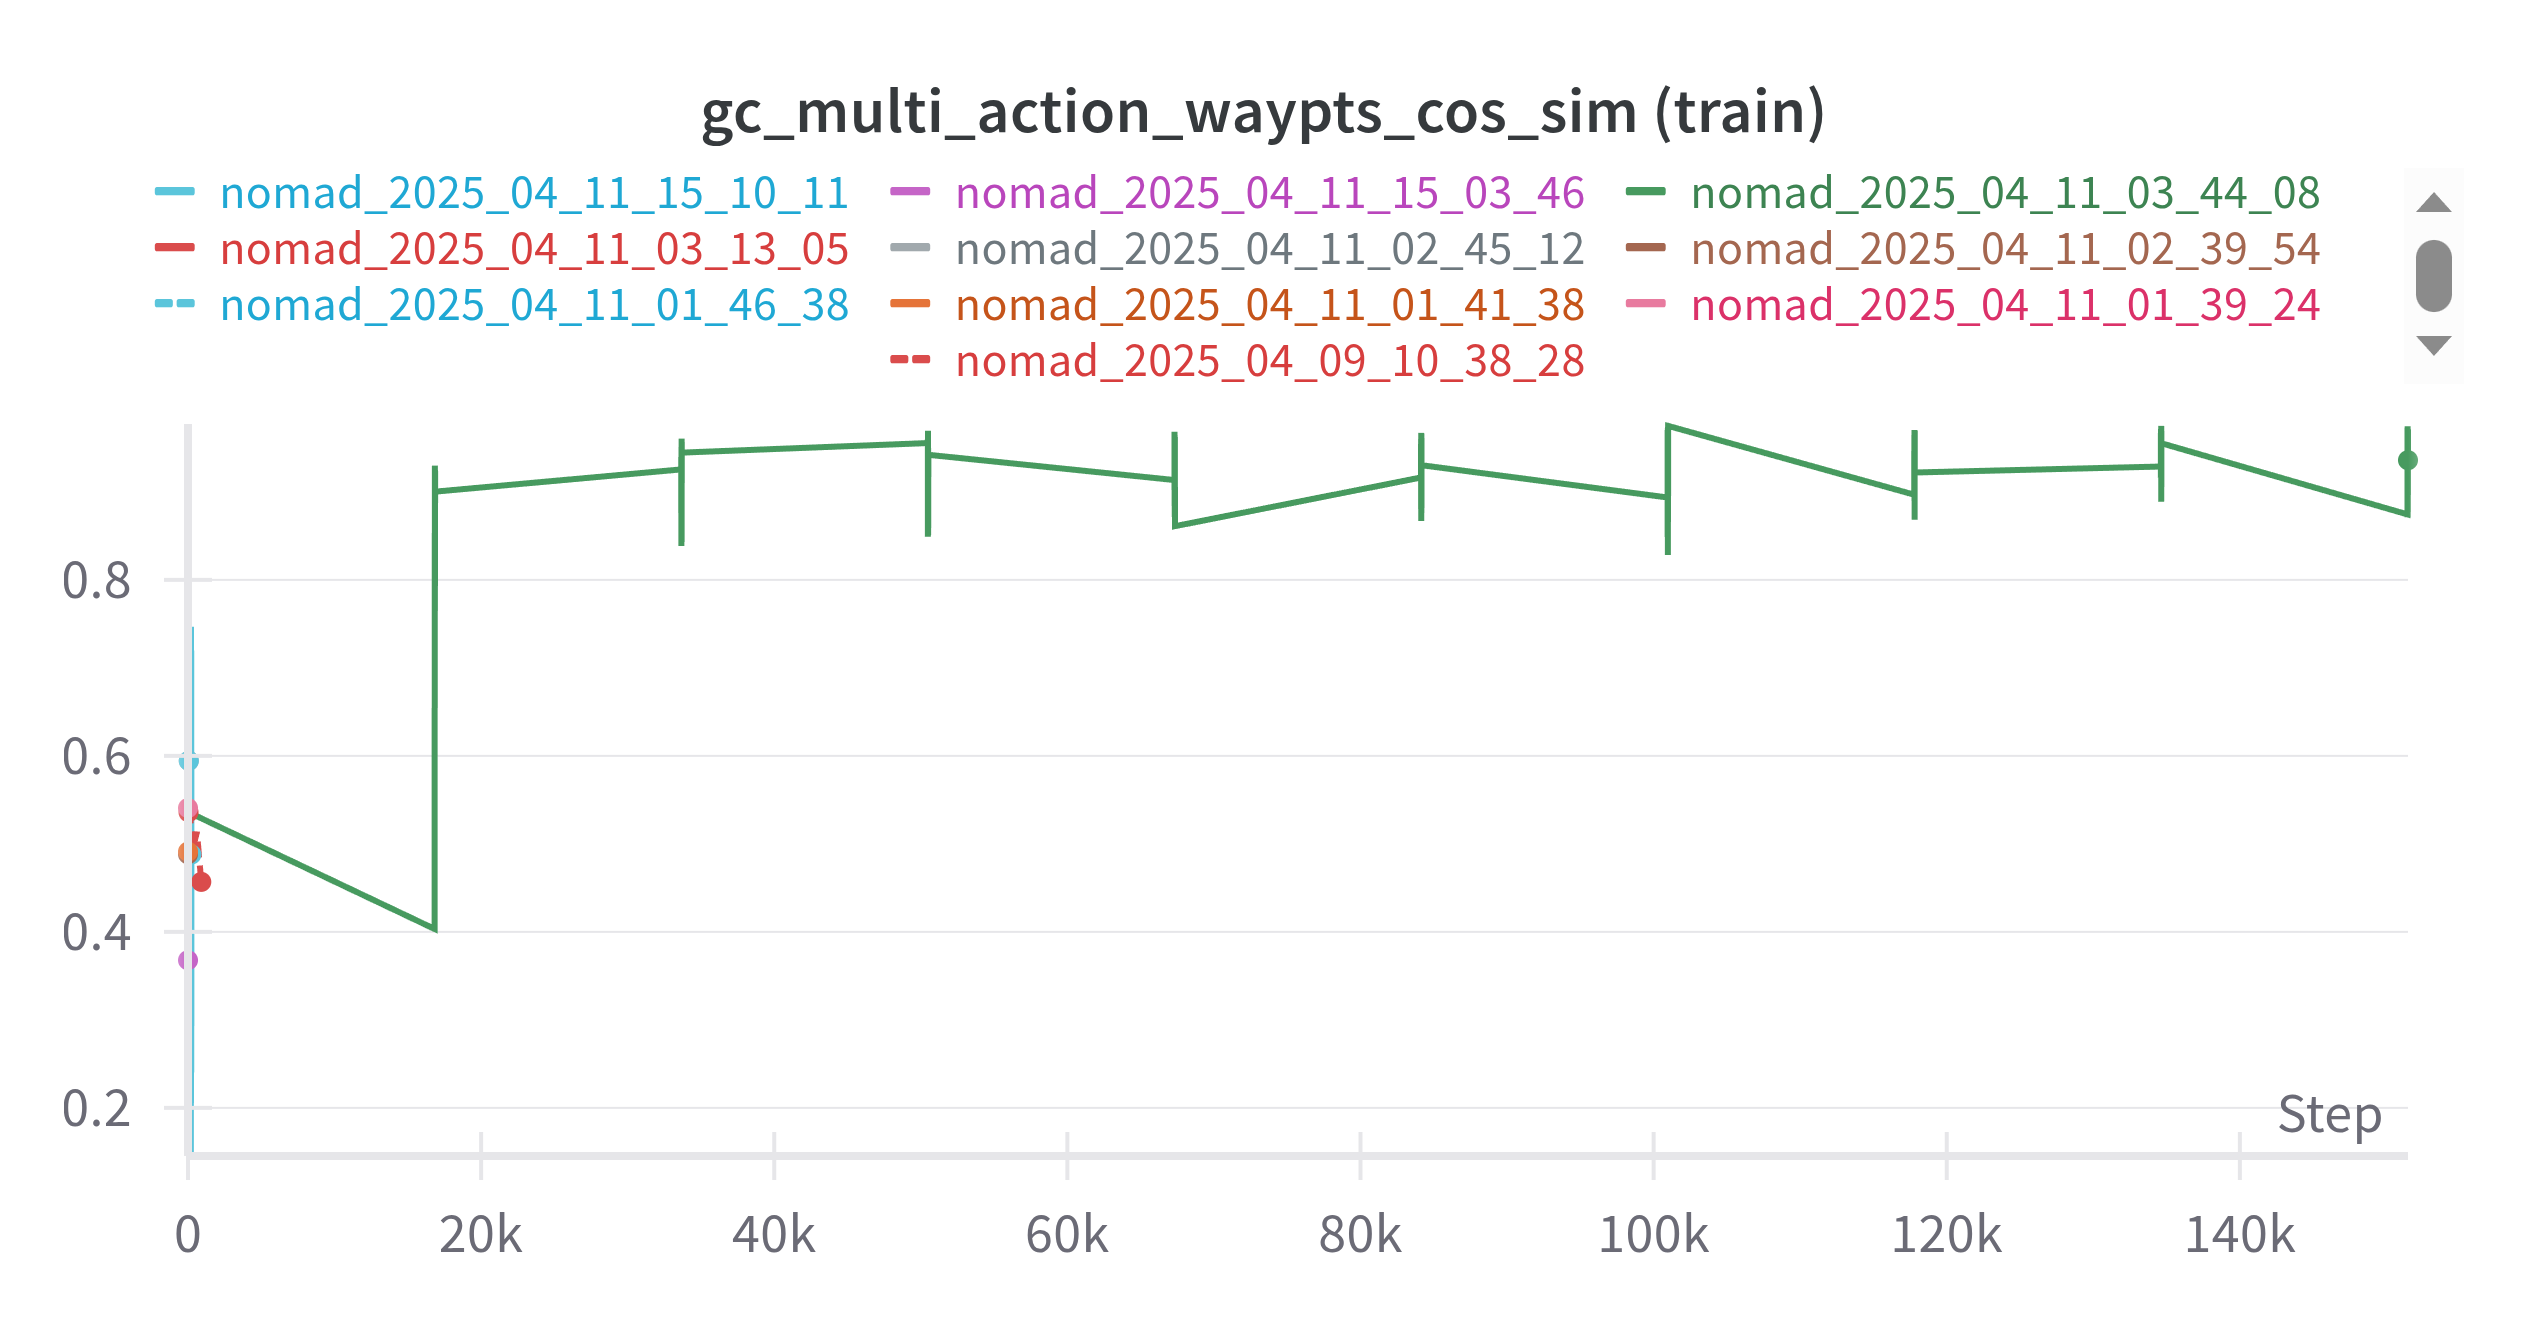
\includegraphics[width=\textwidth]{images/gc_multi_action_waypts_cos_sim.png}
        \caption{Cosine Similarity on Training Set}
        \label{fig:gc_multi_action_waypts_cos_sim}
    \end{subfigure}
    \hfill
    \begin{subfigure}[b]{0.48\textwidth}
        \centering
        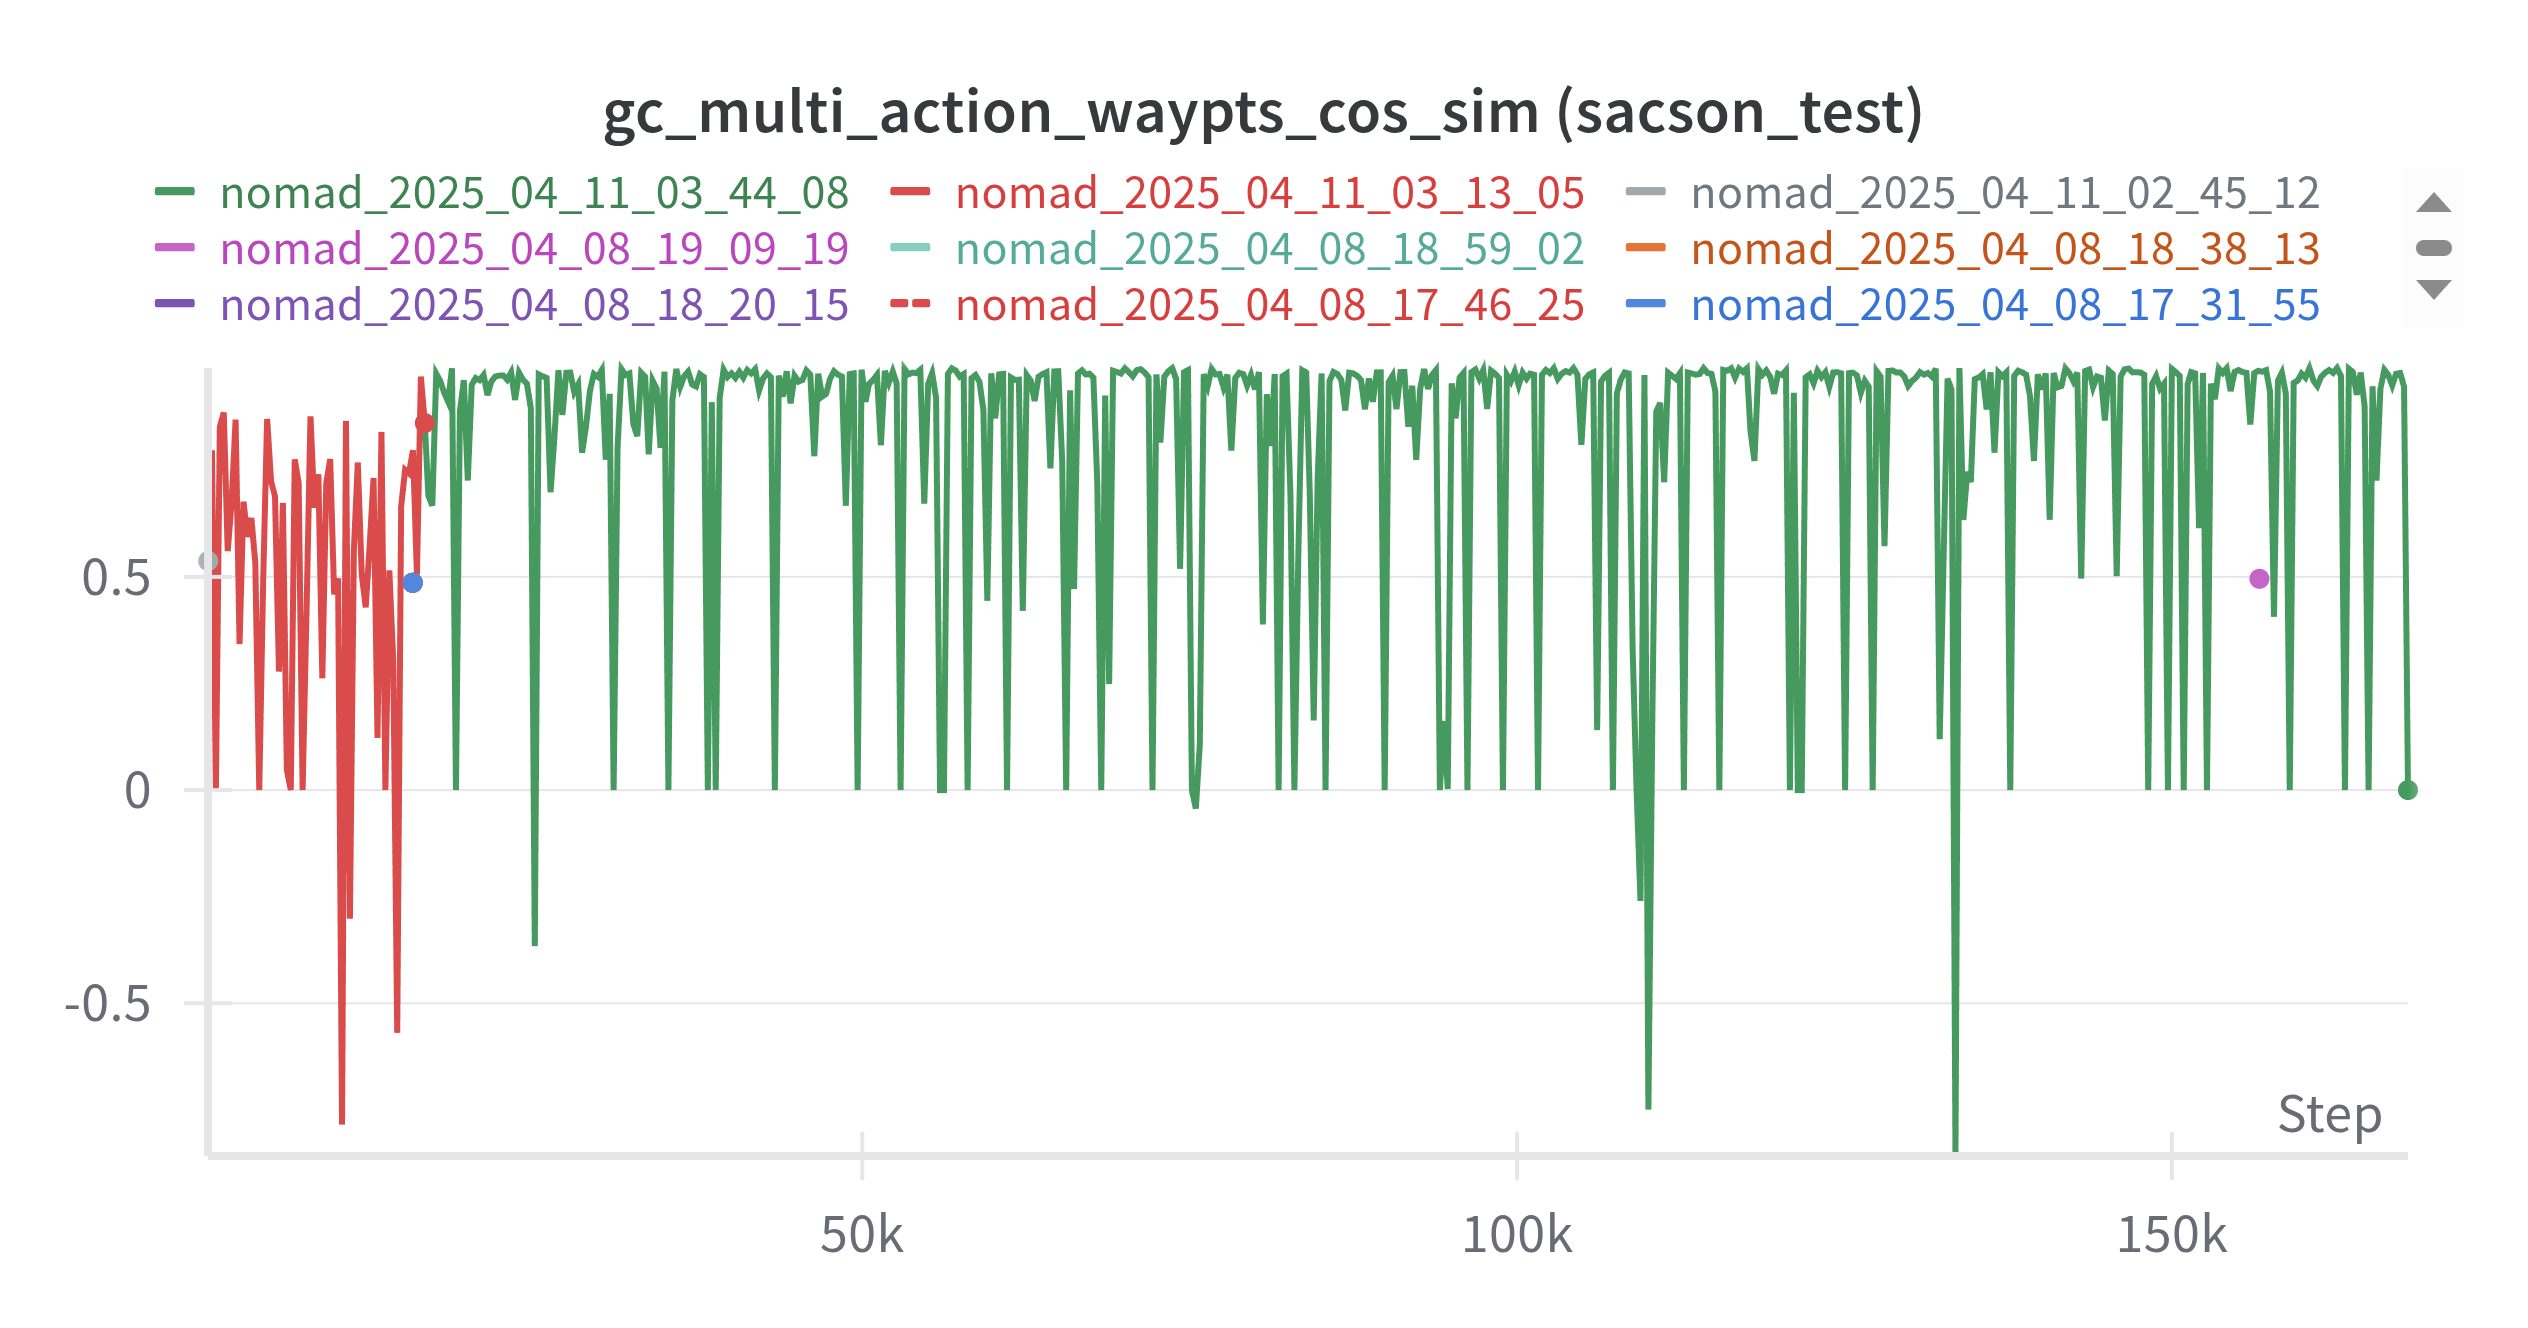
\includegraphics[width=\textwidth]{images/gc_multi_action_waypts_cos_sim_test.png}
        \caption{Cosine Similarity on Validation Set}
        \label{fig:gc_action_multi_waypts_cos_sim_test}
    \end{subfigure}
    \caption{Cosine similarity between predicted and ground-truth multi-waypoints on the training and validation sets under goal-conditioned evaluation.}
\end{figure}
Multi-action cosine similarity compares the overall alignment of full predicted trajectory vectors with ground truth, rather than frame-by-frame. This provides a more holistic measure of long-horizon trajectory quality.
We see a similar trend in multi-action cosine similarity as action waypts cosine similarity. On the training set, the plot consistently improves and stabilizes at a high value, indicating that the model effectively learns to align its predicted trajectories with the desired paths. Similarly we notice the lower and more volatile cosine similarity on the validation set.
\newpage
\subsection*{Unconditional (UC) Evaluation}
We set the goal mask $m = 1$ to evaluate the model's performance in open-ended exploration.\\
Interestingly, the model's behavior in this unconditioned setting closely mirrors that observed during goal-conditioned evaluations. This indicates that the model encounters similar generalization challenges and follows comparable learning dynamics, even in the absence of explicit goal cues.\\
\noindent \textbf{Action loss:}\\
\begin{figure}[H]
    \centering
    \begin{subfigure}[b]{0.48\textwidth}
        \centering
        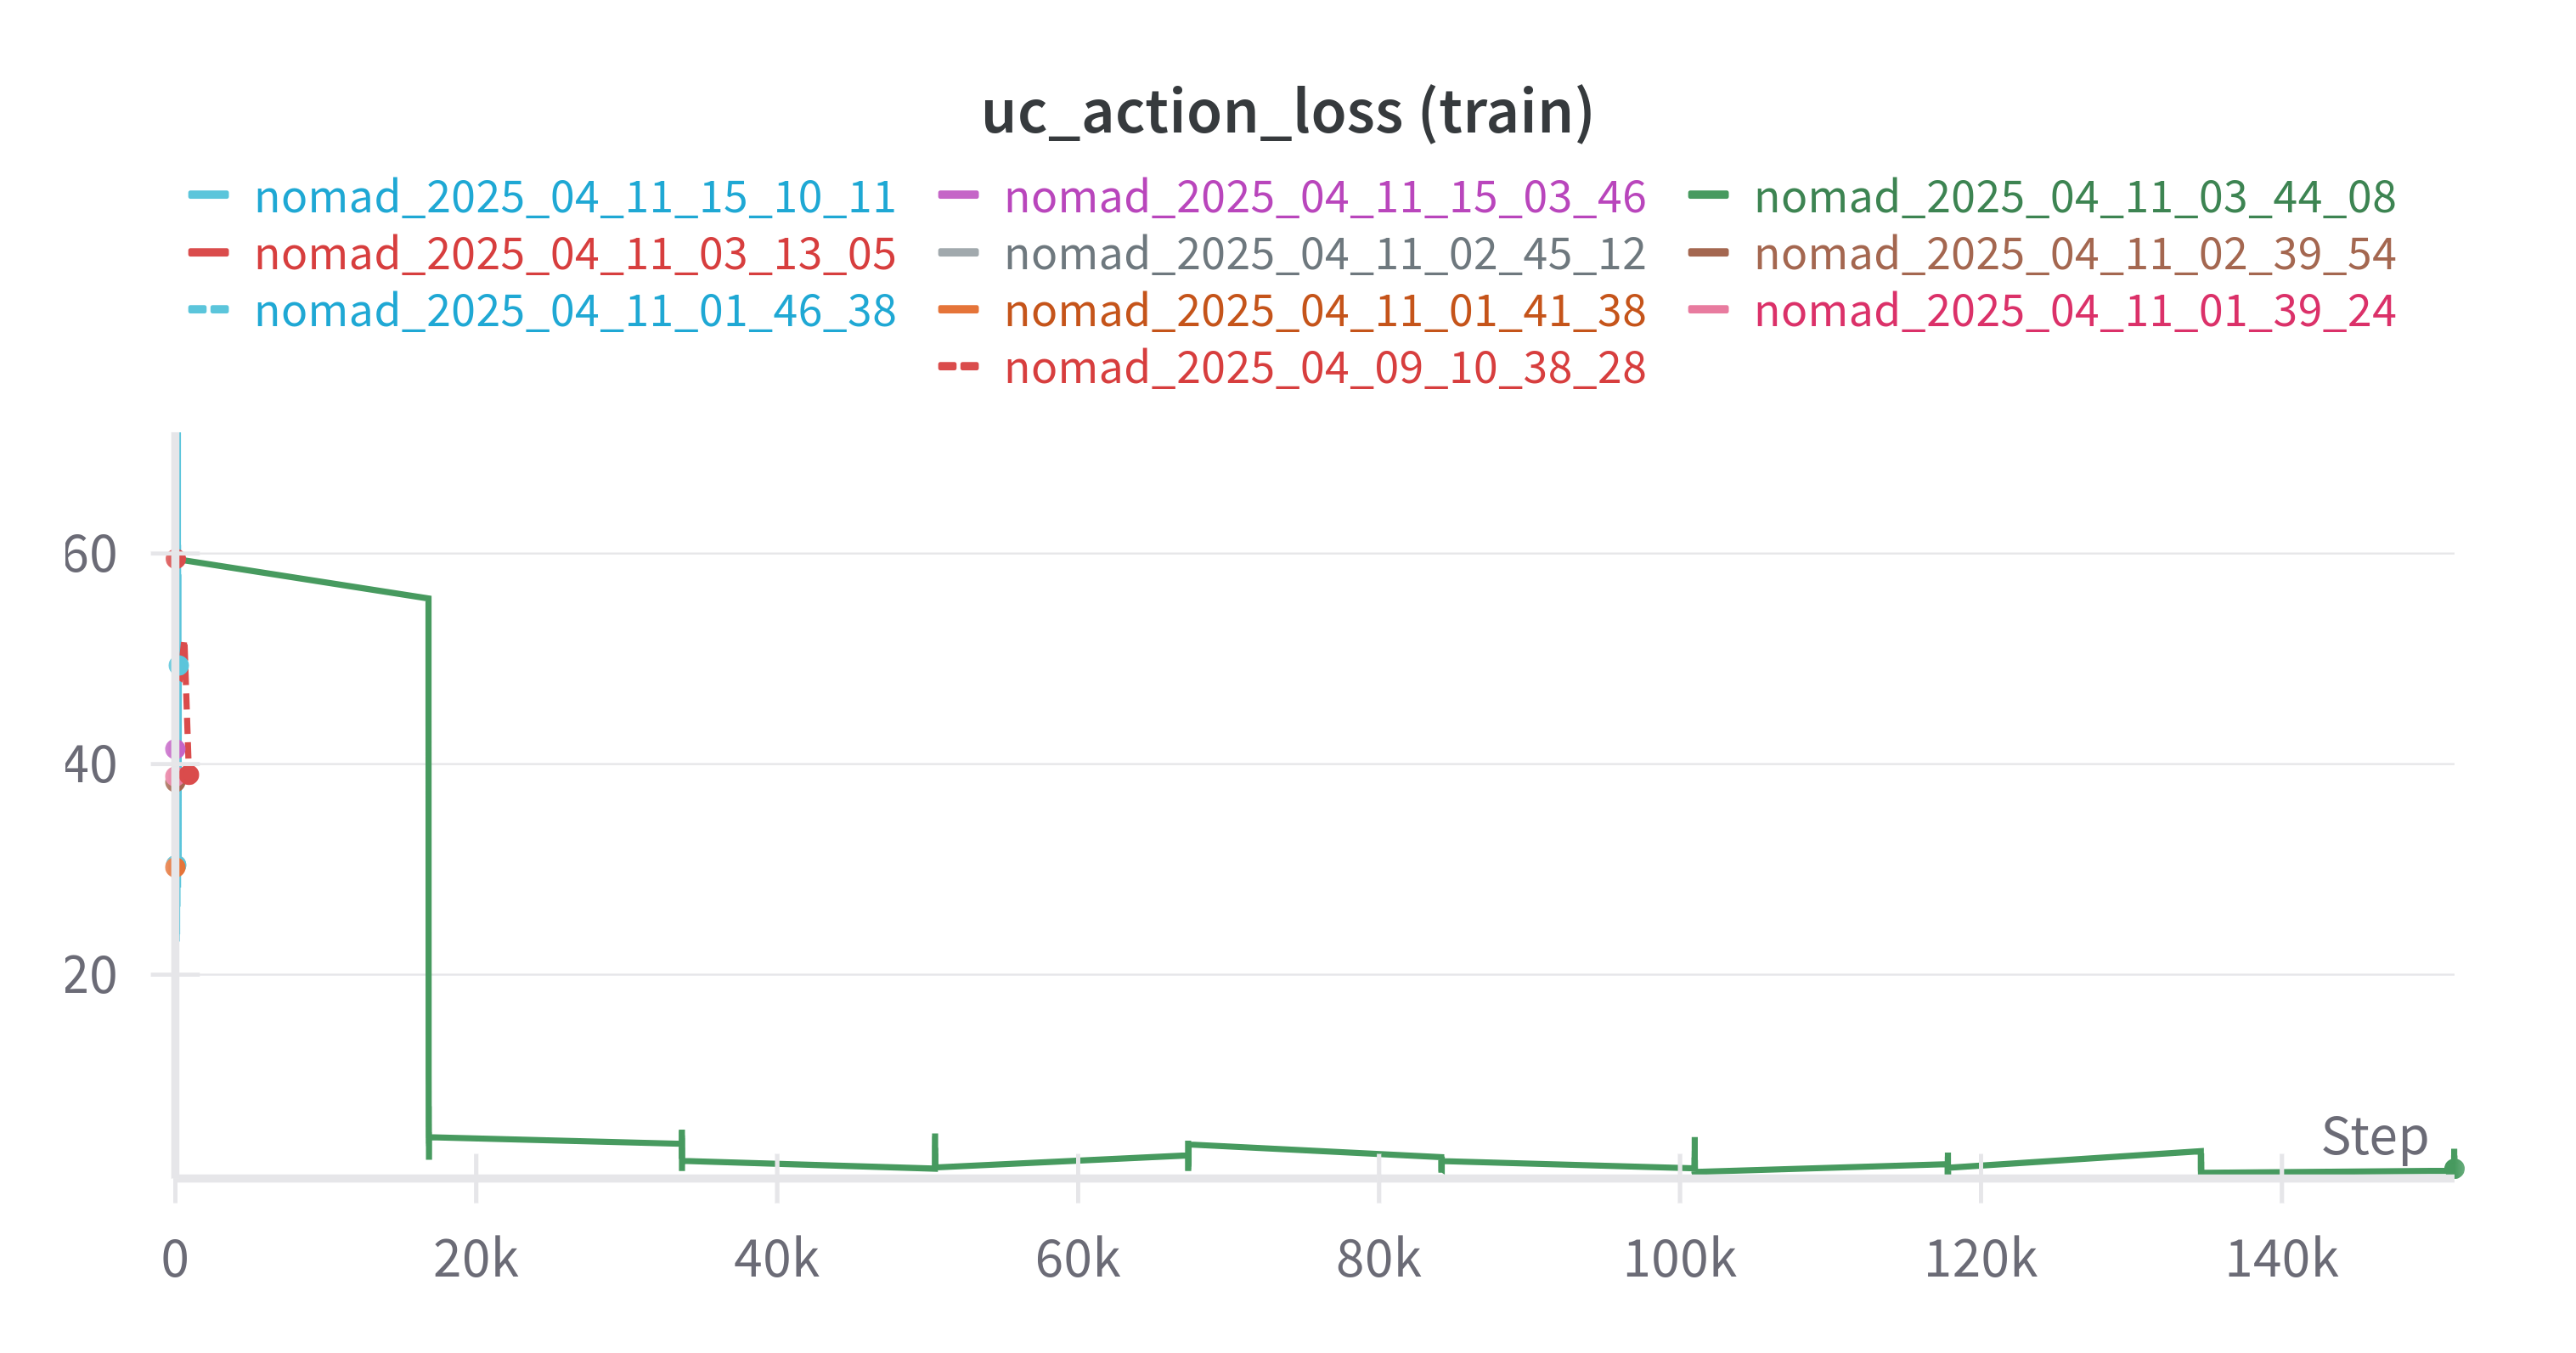
\includegraphics[width=\textwidth]{images/uc_action_train.png}
        \caption{Action Loss on Training Set}
        \label{fig:gc_action_loss_train}
    \end{subfigure}
    \hfill
    \begin{subfigure}[b]{0.48\textwidth}
        \centering
        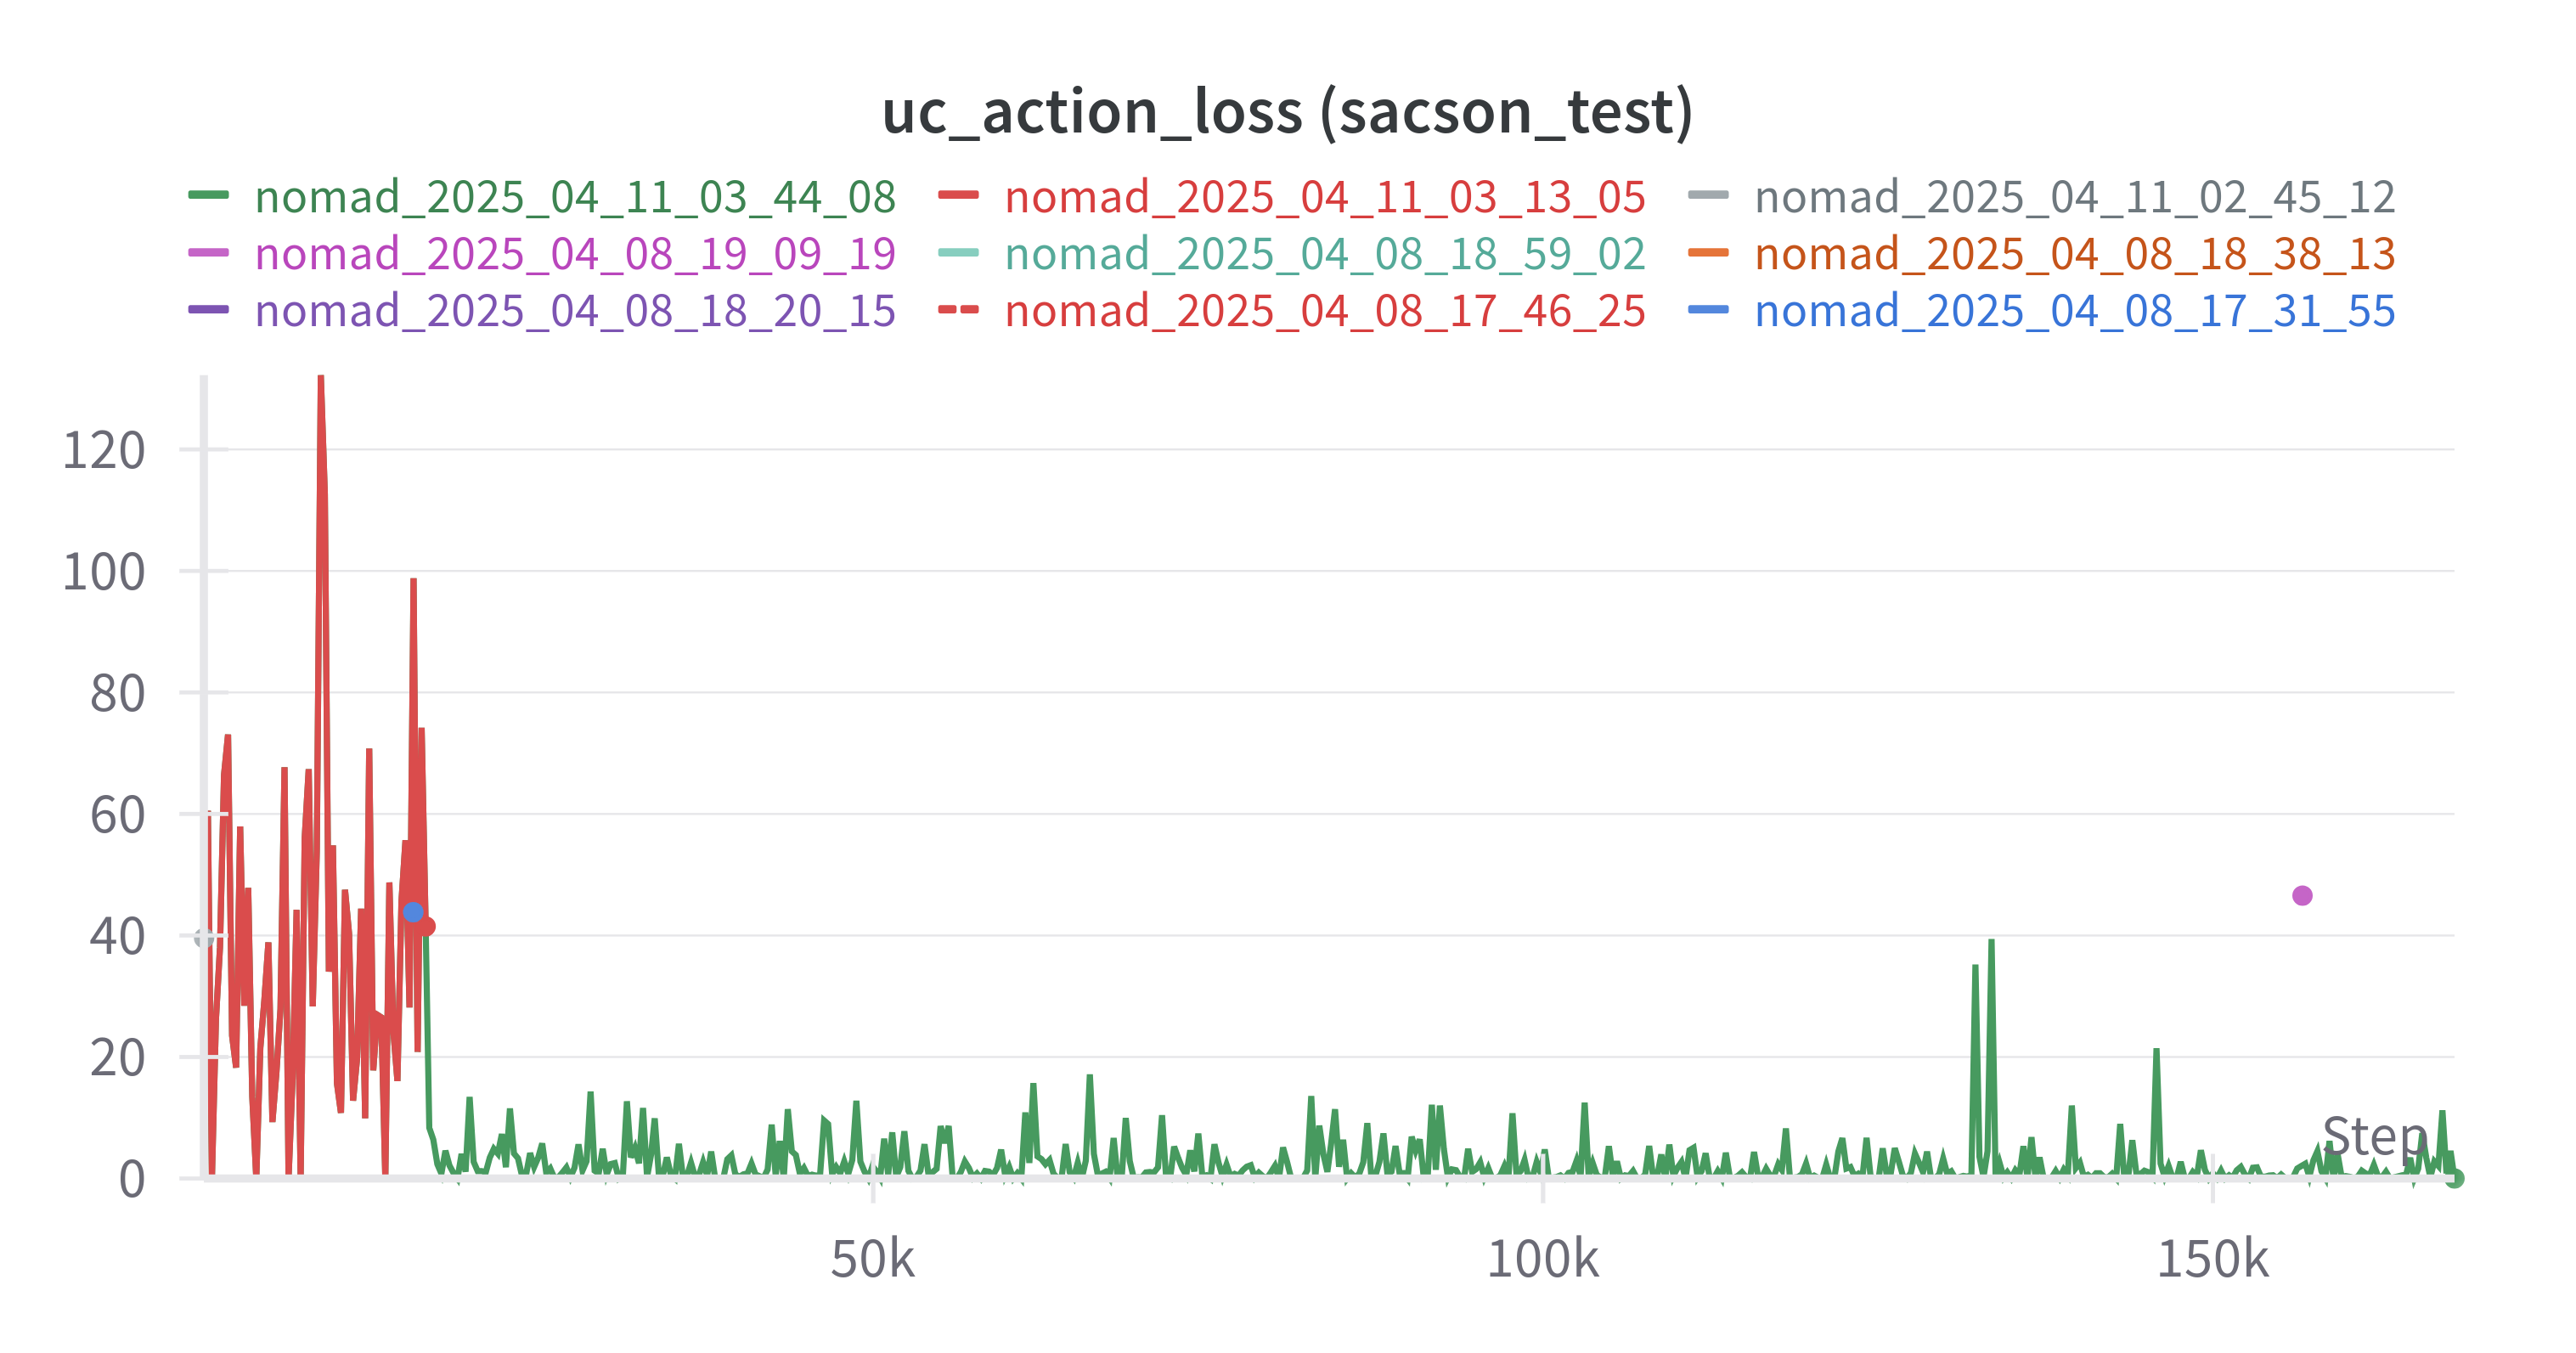
\includegraphics[width=\textwidth]{images/uc_action_test.png}
        \caption{Action Loss on Validation Set}
        \label{fig:gc_action_loss_val}
    \end{subfigure}
    \caption{Action loss comparison between training and validation sets under goal-agnostic evaluation.}
\end{figure}
\noindent \textbf{uc\_action\_waypts\_cos\_sim:}\\
\begin{figure}[H]
    \centering
    \begin{subfigure}[b]{0.48\textwidth}
        \centering
        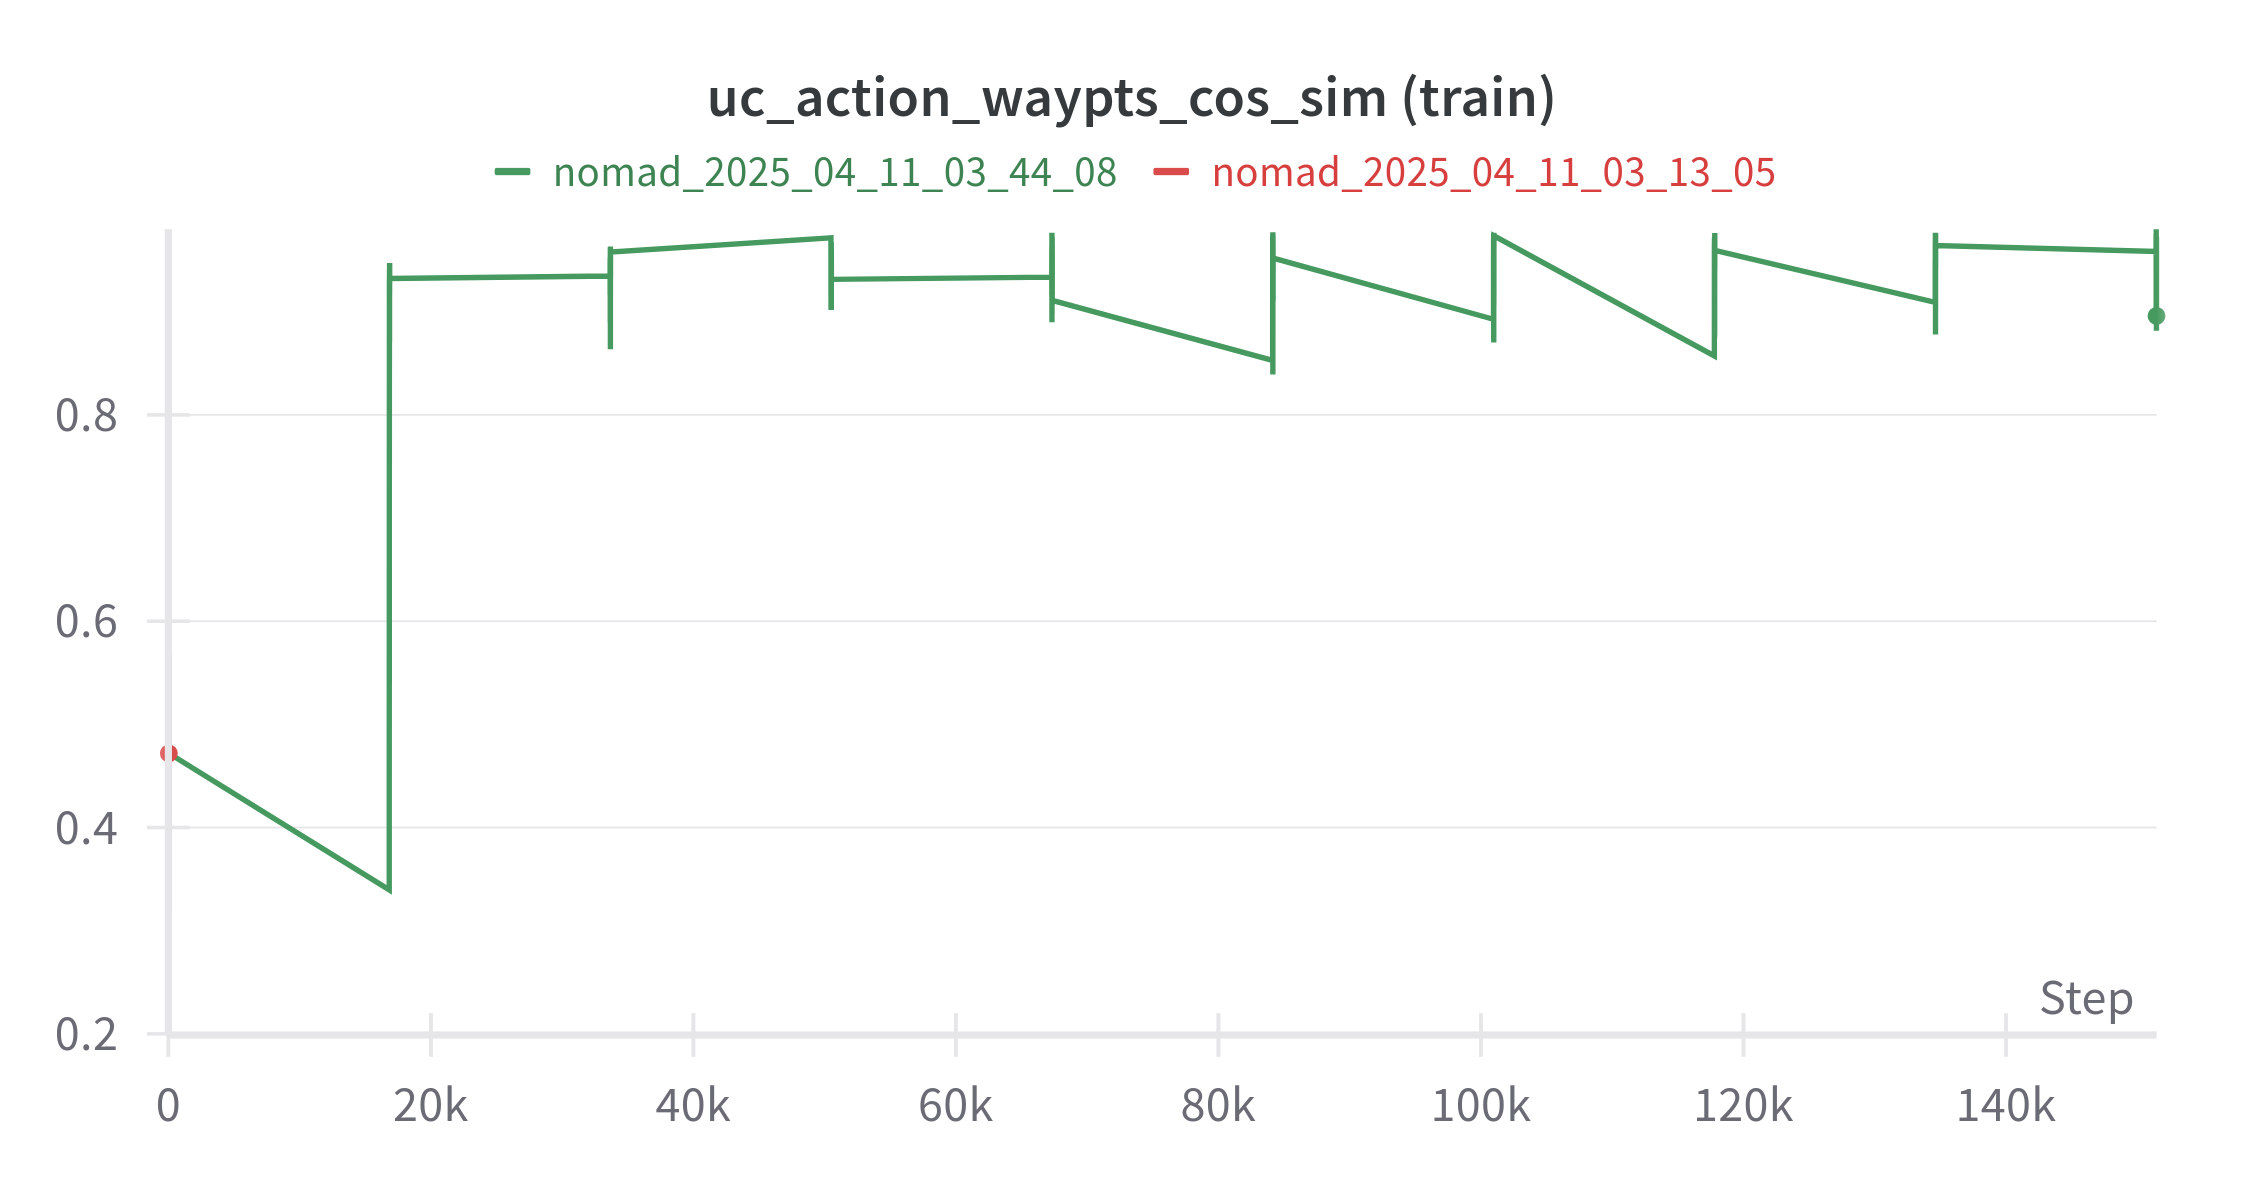
\includegraphics[width=\textwidth]{images/uc_action_sim_train(1).png}
        \caption{Cosine Similarity on Training Set}
        \label{fig:uc_action_waypts_cos_sim_train}
    \end{subfigure}
    \hfill
    \begin{subfigure}[b]{0.48\textwidth}
        \centering
        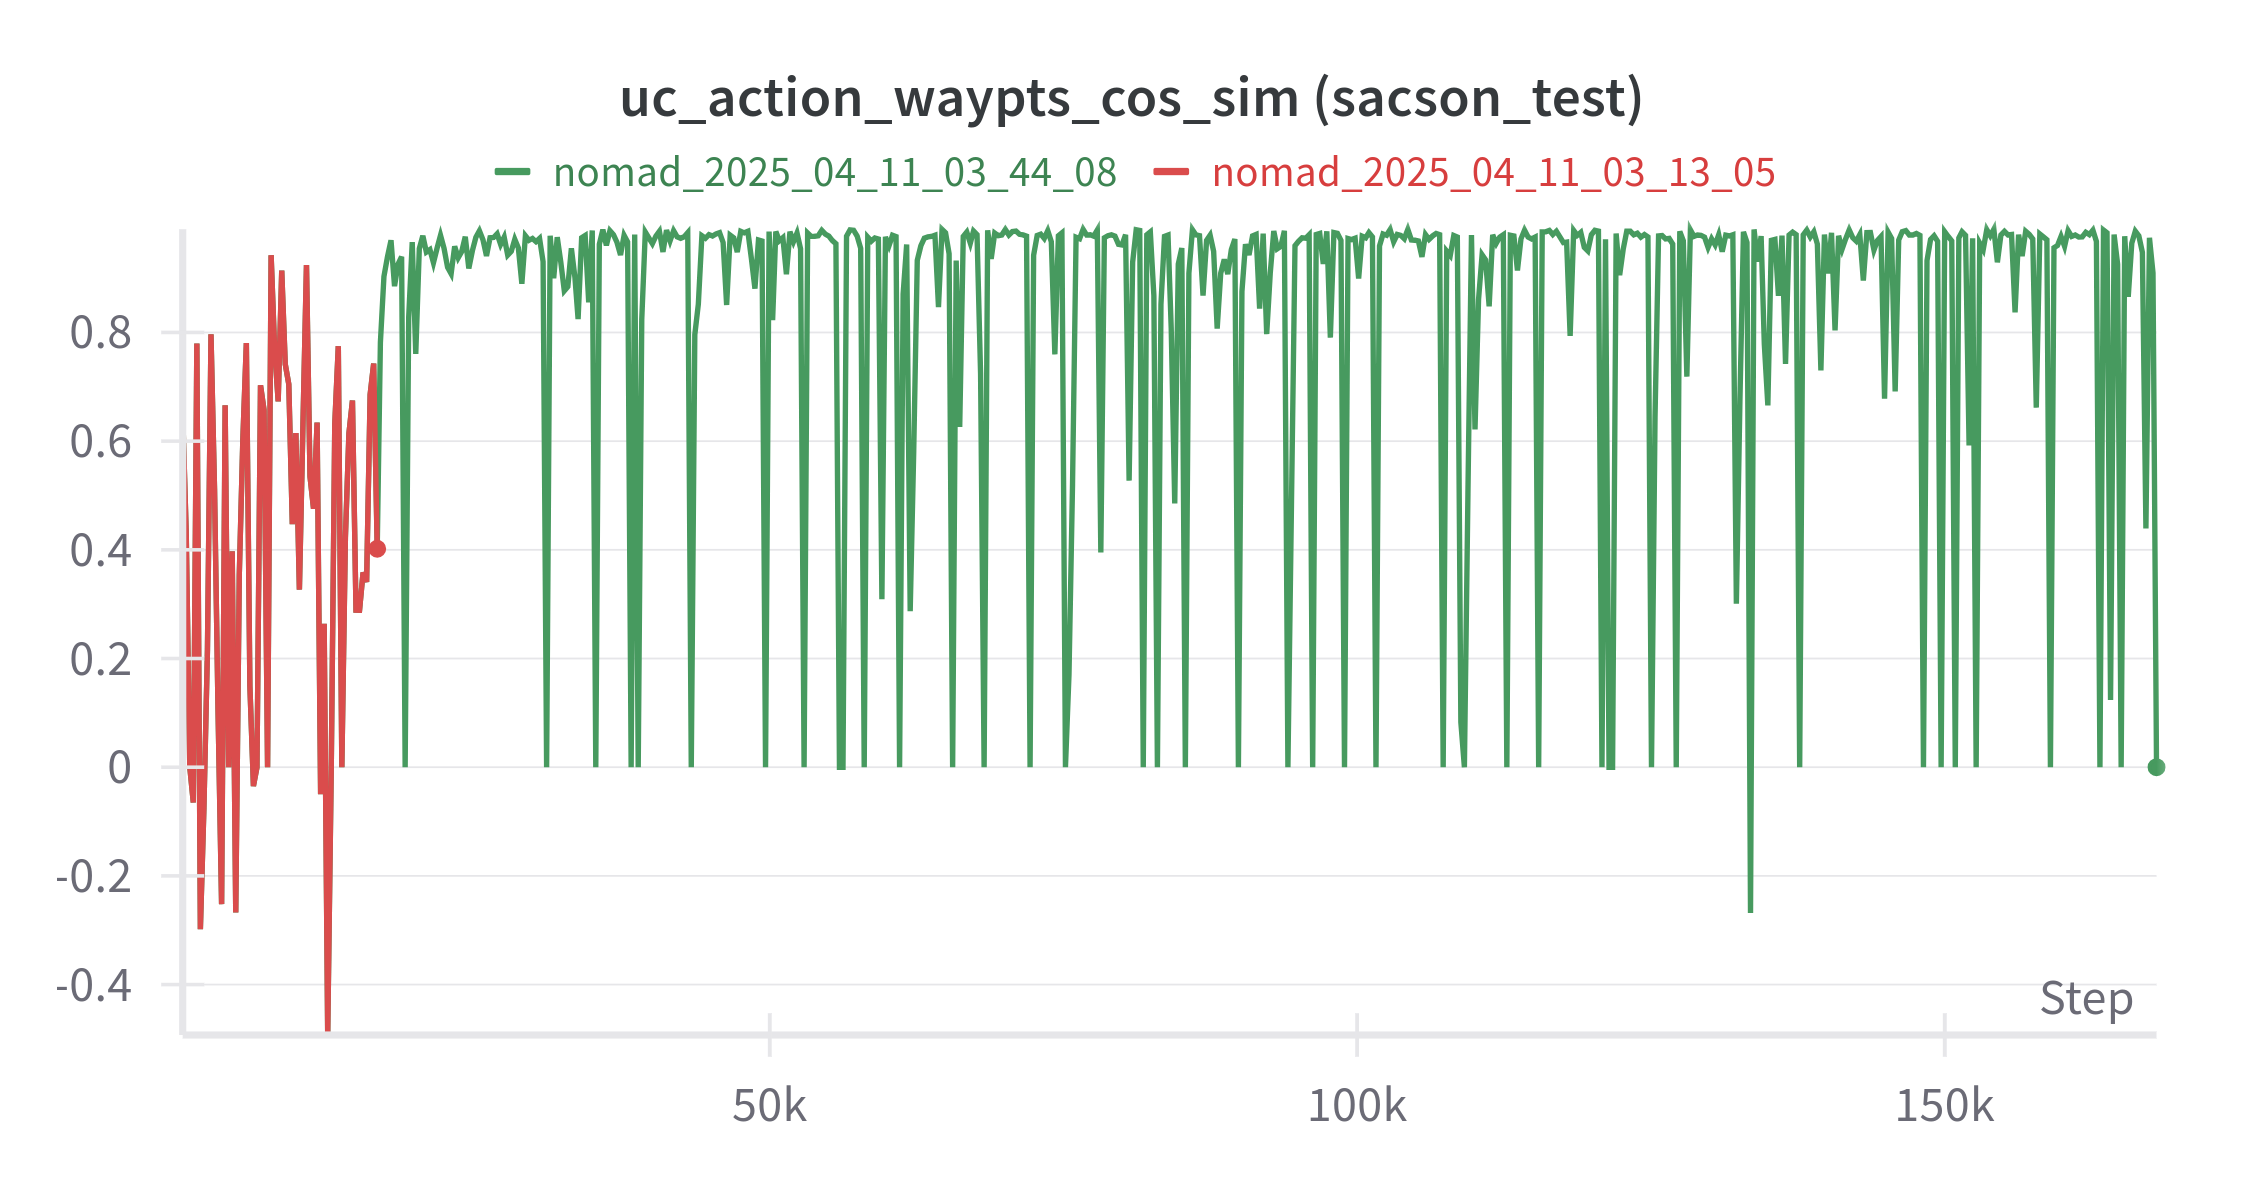
\includegraphics[width=\textwidth]{images/uc_action_sim_test.png}
        \caption{Cosine Similarity on Validation Set}
        \label{fig:uc_action_waypts_cos_sim_val}
    \end{subfigure}
    \caption{Cosine similarity between predicted and ground-truth waypoints on the training and validation sets under goal-agnostic evalutation}
\end{figure}
\newpage
\noindent \textbf{uc\_multi\_action\_waypts\_cos\_sim:}\\
\begin{figure}[H]
    \centering
    \begin{subfigure}[b]{0.48\textwidth}
        \centering
        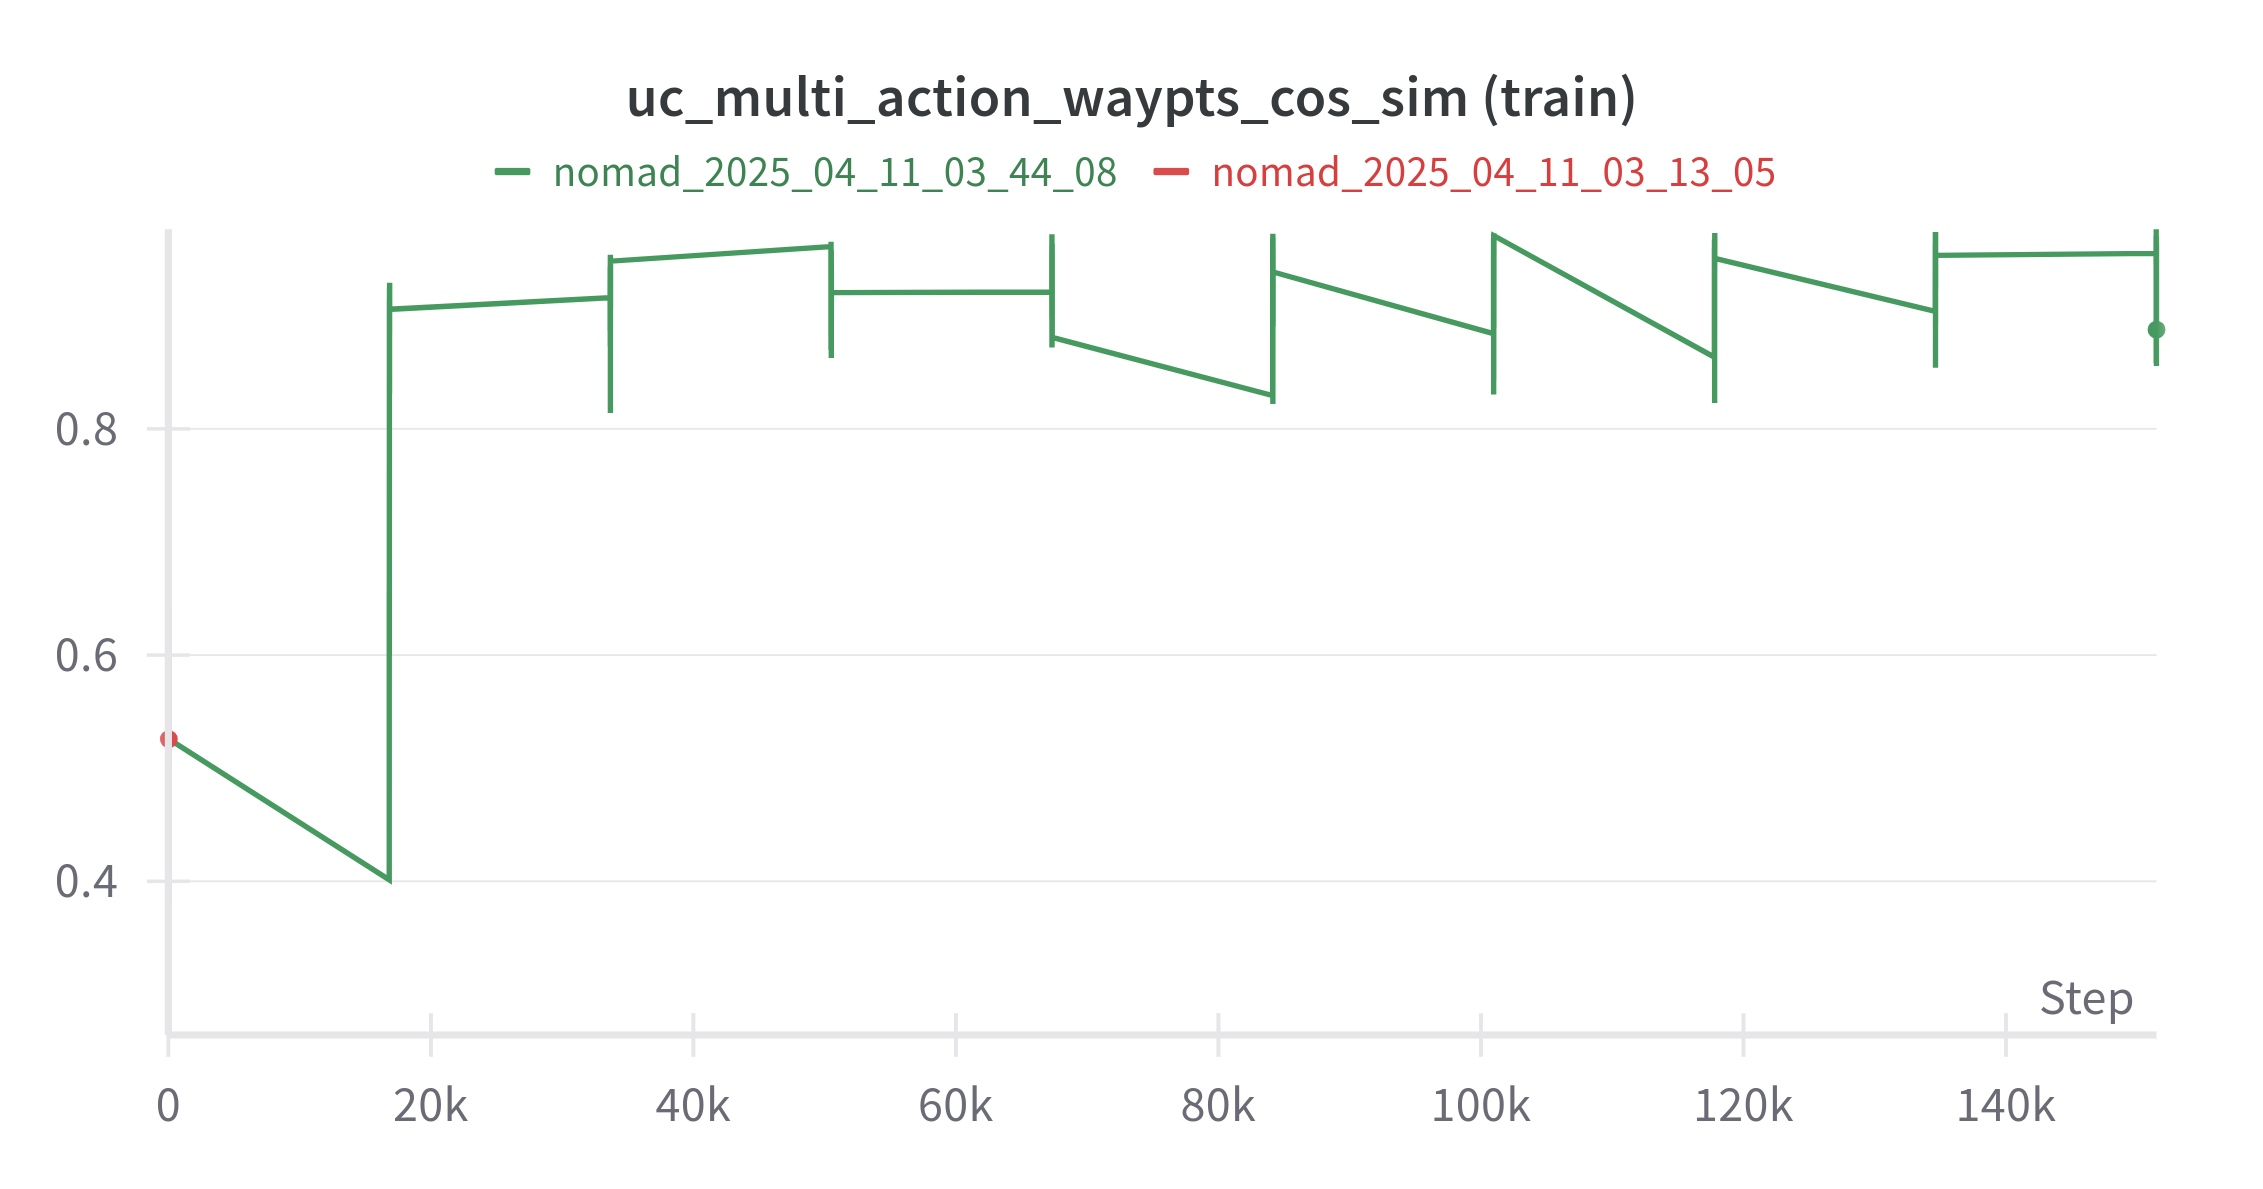
\includegraphics[width=\textwidth]{images/cs_multi_action_cos_train.png}
        \label{fig:uc_multi_action_waypts_cos_sim}
    \end{subfigure}
    \hfill
    \begin{subfigure}[b]{0.48\textwidth}
        \centering
        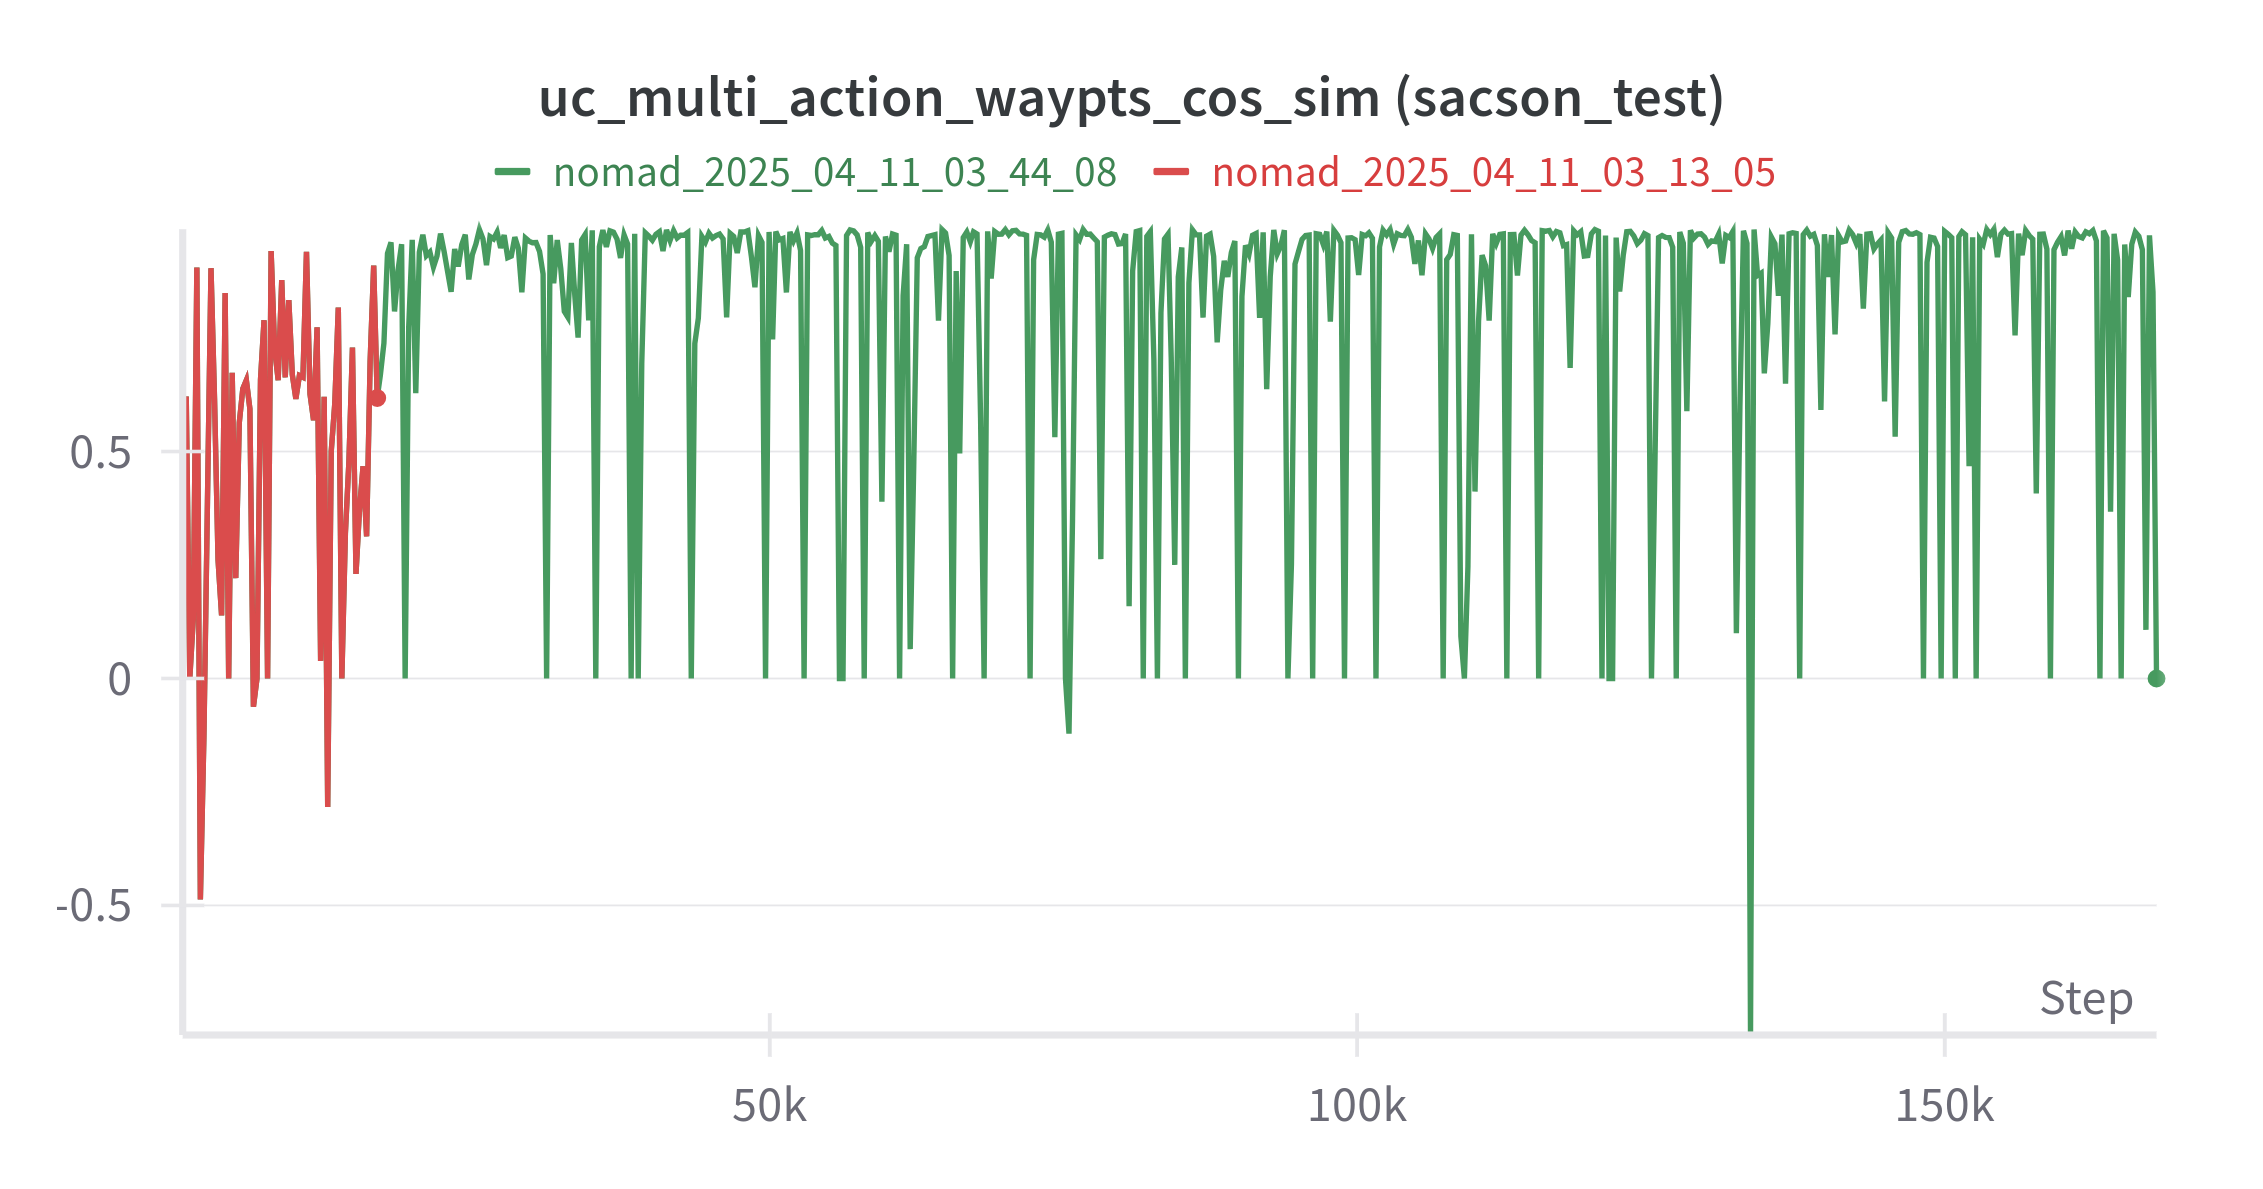
\includegraphics[width=\textwidth]{images/uc_multi_action_sim_test.png}
        \caption{Cosine Similarity on Validation Set}
        \label{fig:uc_action_multi_waypts_cos_sim_test}
    \end{subfigure}
    \caption{Cosine similarity between predicted and ground-truth multi-waypoints on the training and validation sets under goal-agnostic evalutation}
\end{figure}
\bigskip
\noindent \textbf{Distance Loss:}\\
\begin{figure}[H]
    \centering
    \begin{subfigure}[b]{0.8\textwidth}
        \centering
        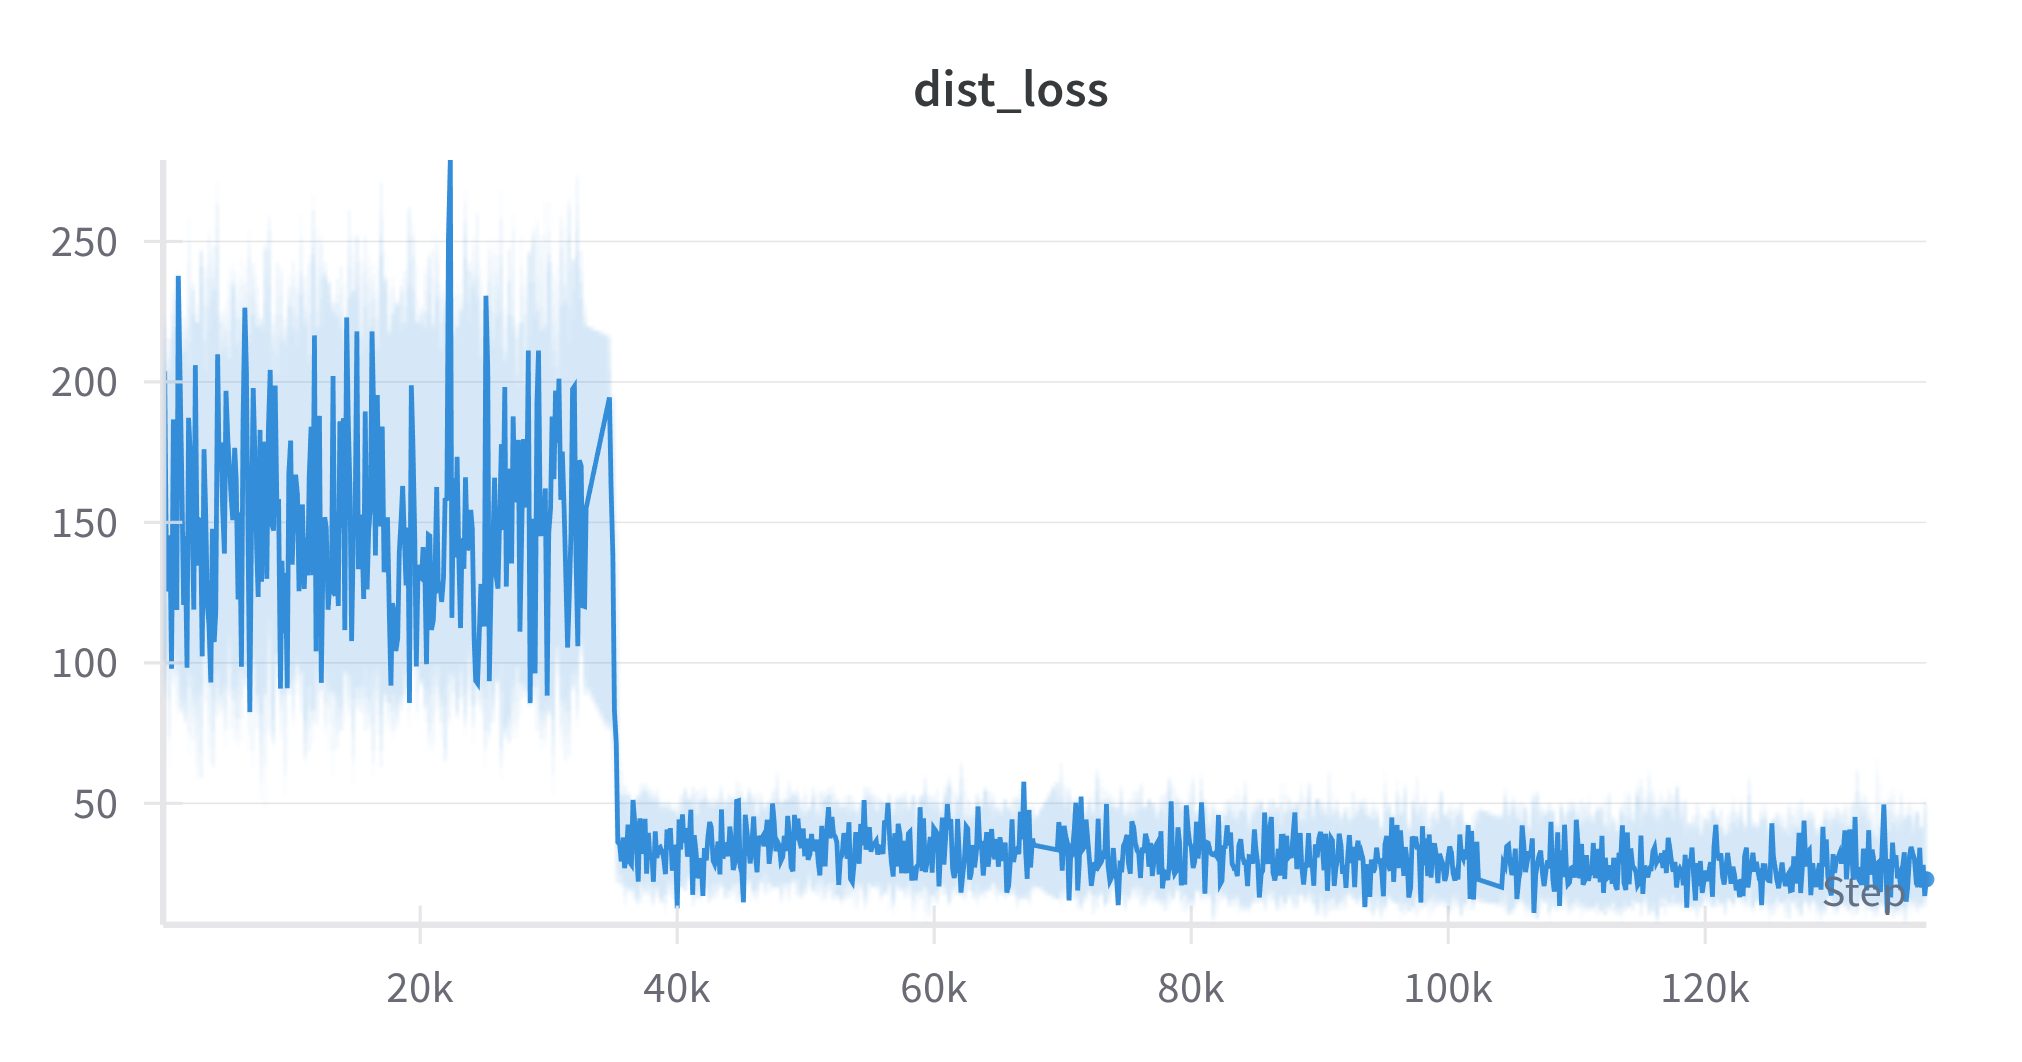
\includegraphics[width=\textwidth]{images/dist_loss.png}
        \caption{Distance Loss on Training Set}
        \label{fig:dist_loss}
    \end{subfigure}
    \end{figure}
    Figure \ref{fig:dist_loss} illustrates the variation in distance loss over the course of training steps. The sharp drop in loss around 35k steps marks a point where the model begins to learn more effectively. The loss stabilizes at a low value in the later stages, indicating that the model has successfully converged to a well-optimized solution for the training data. This reduction in uncertainty further suggests that the learning process has become more consistent and efficient.\\
\subsection*{Diffusion Loss}
\begin{figure}[H]
    \centering
    \begin{subfigure}[b]{0.48\textwidth}
        \centering
        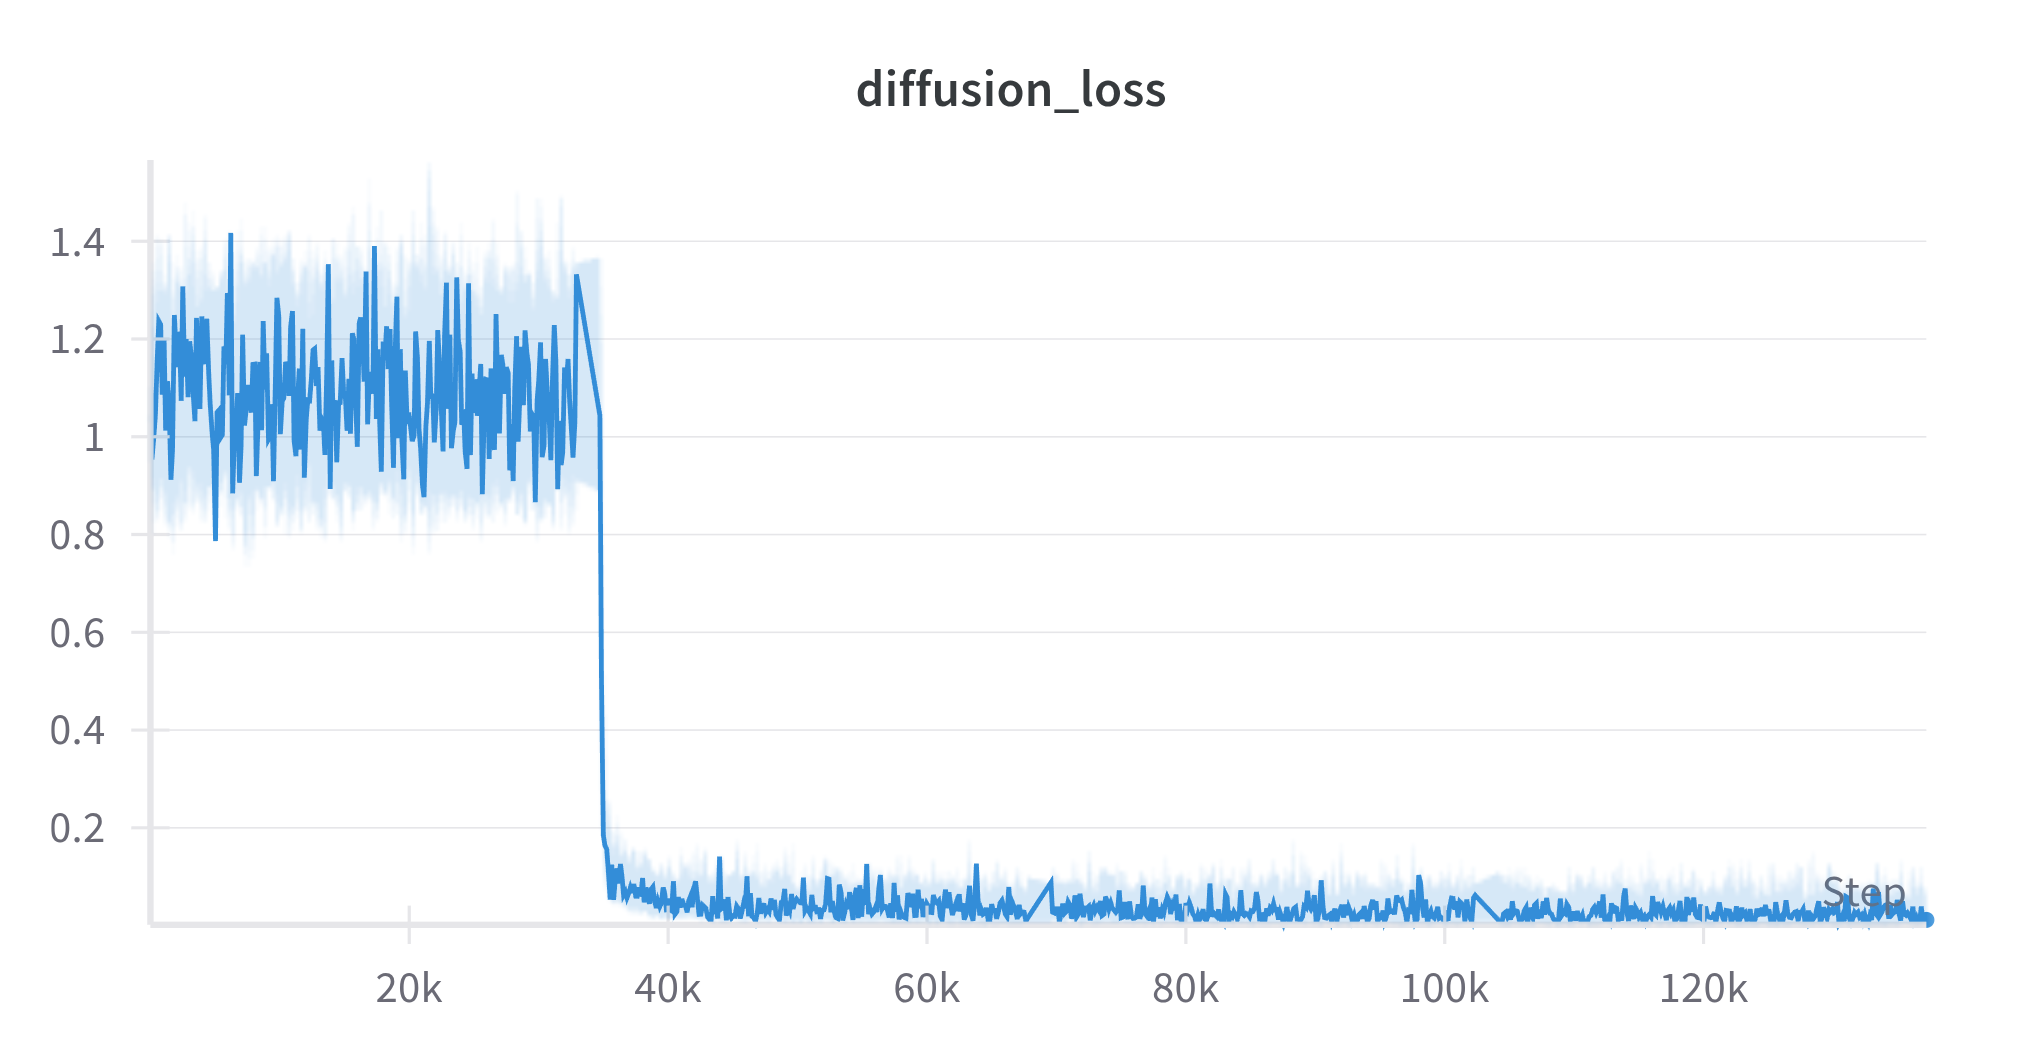
\includegraphics[width=\textwidth]{images/diffusion_loss.png}
        \caption{Diffusion Loss on Training Set}
        \label{fig:diffusion_loss}
    \end{subfigure}
    \hfill
    \begin{subfigure}[b]{0.48\textwidth}
        \centering
        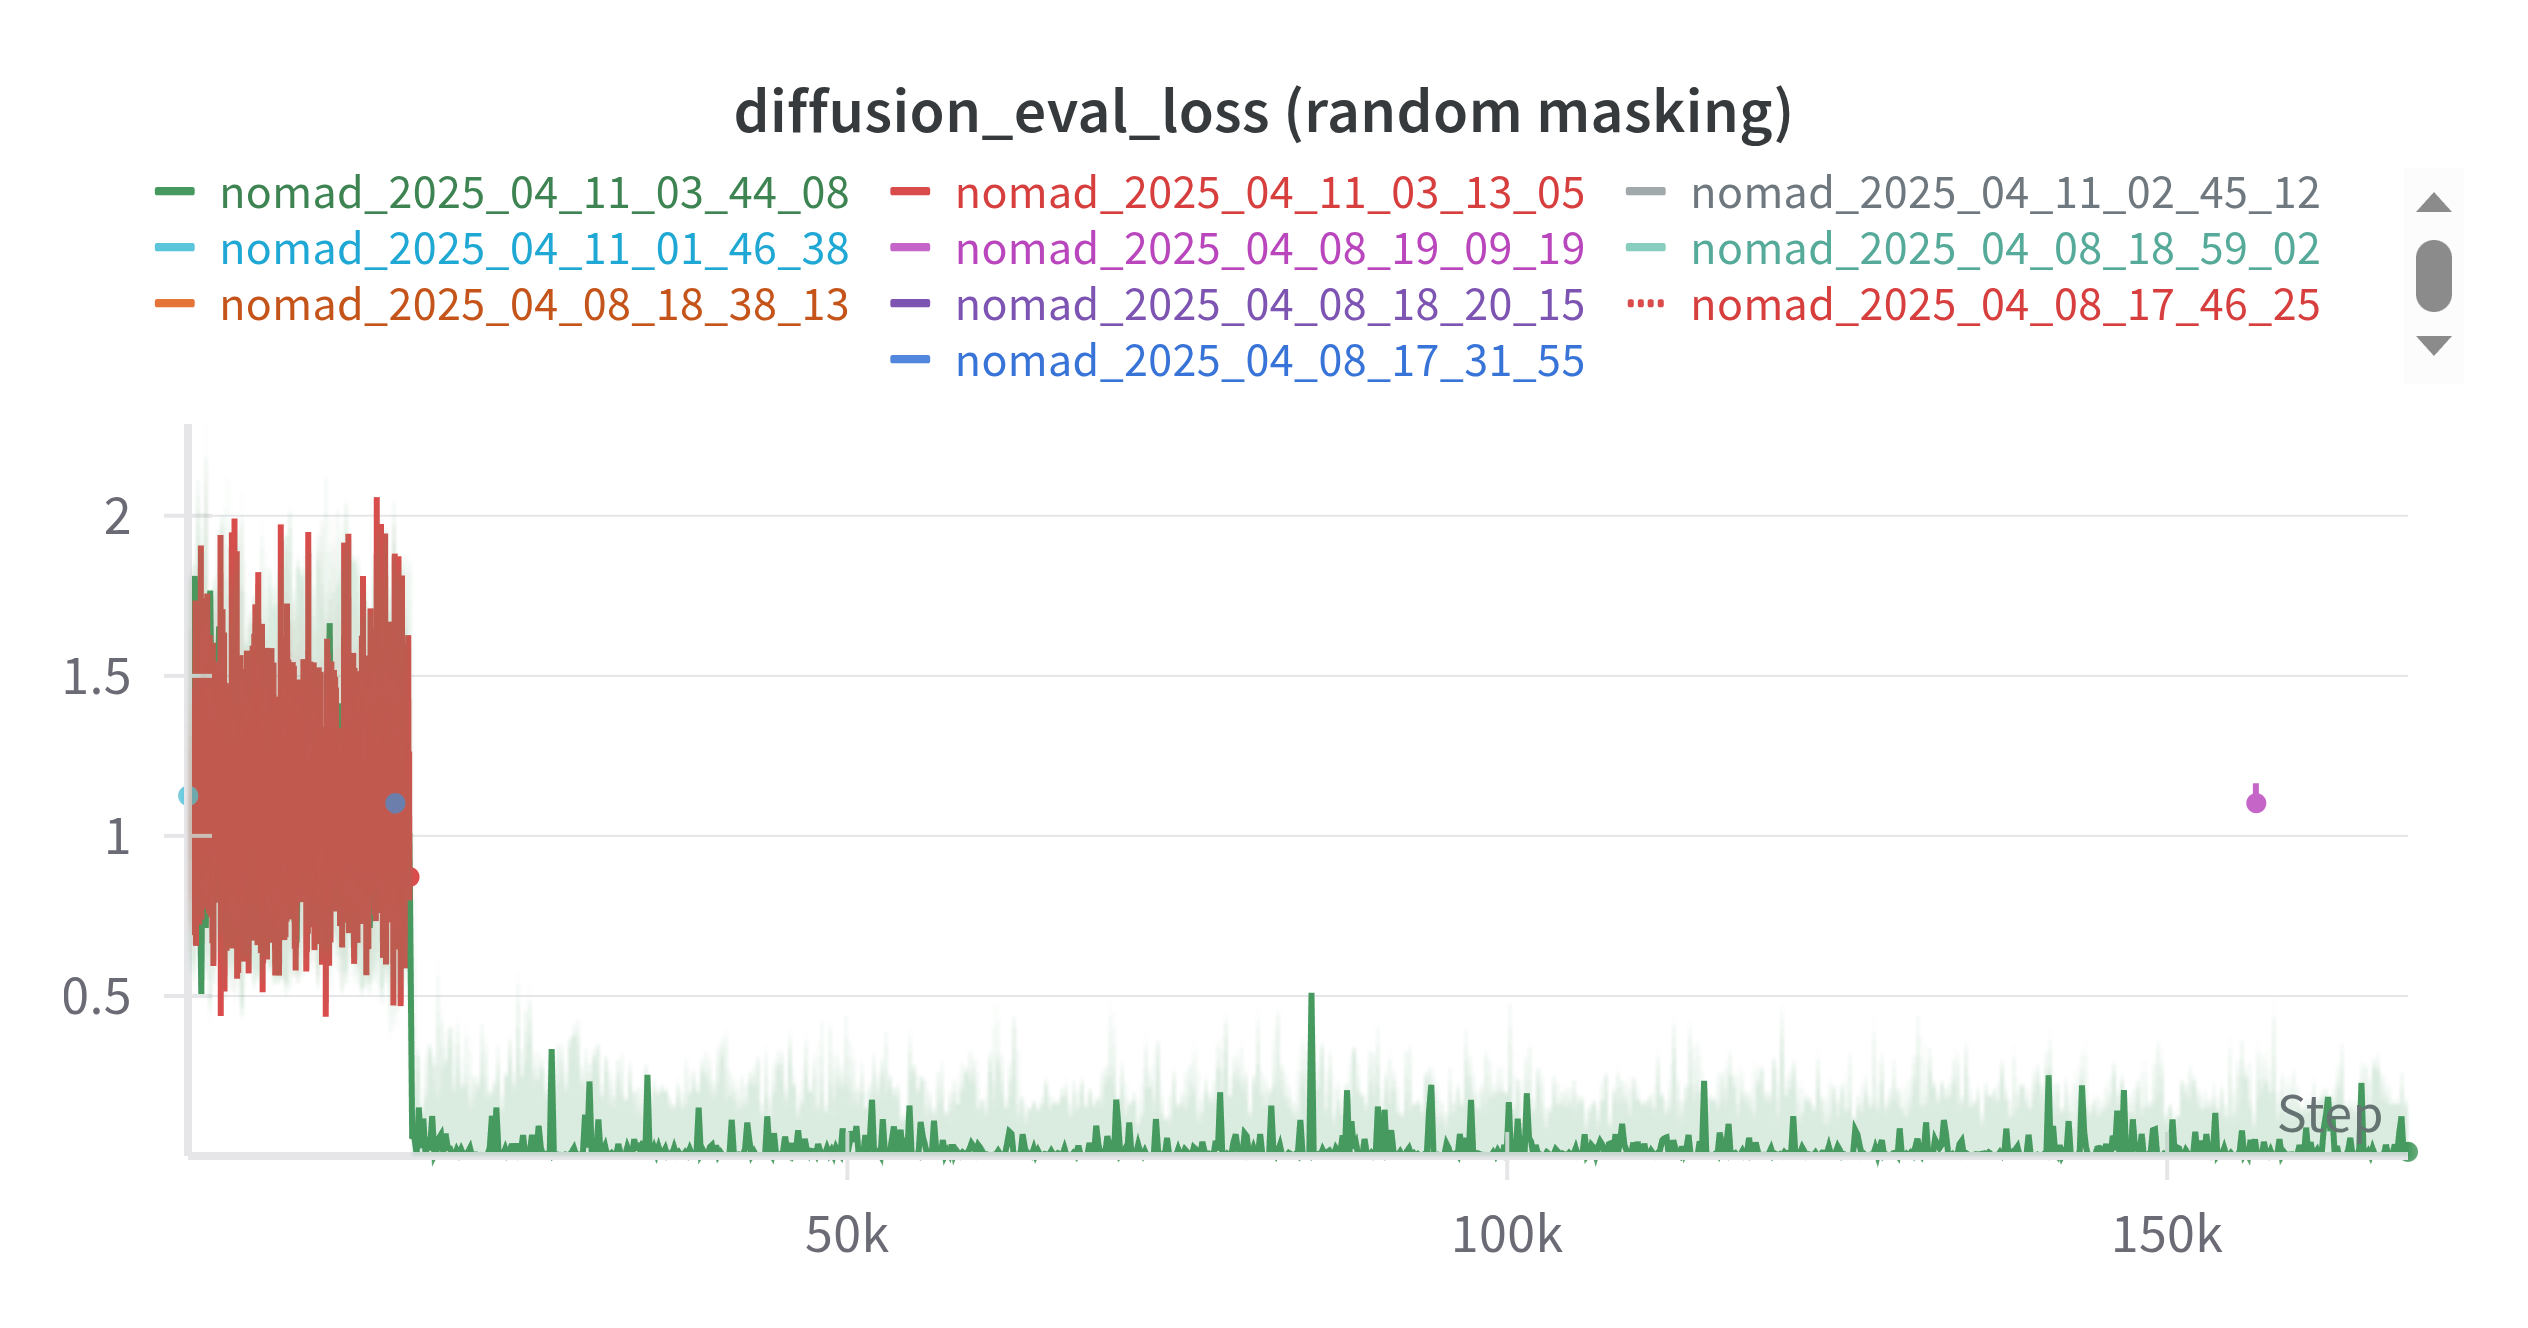
\includegraphics[width=\textwidth]{images/diffusion_eval_loss_random_masking.png}
        \caption{Diffusion evaluation loss with random masking}
        \label{fig:diffusion_eval_loss_random_masking}
    \end{subfigure}
    \begin{subfigure}[H]{0.48\textwidth}
        \centering
        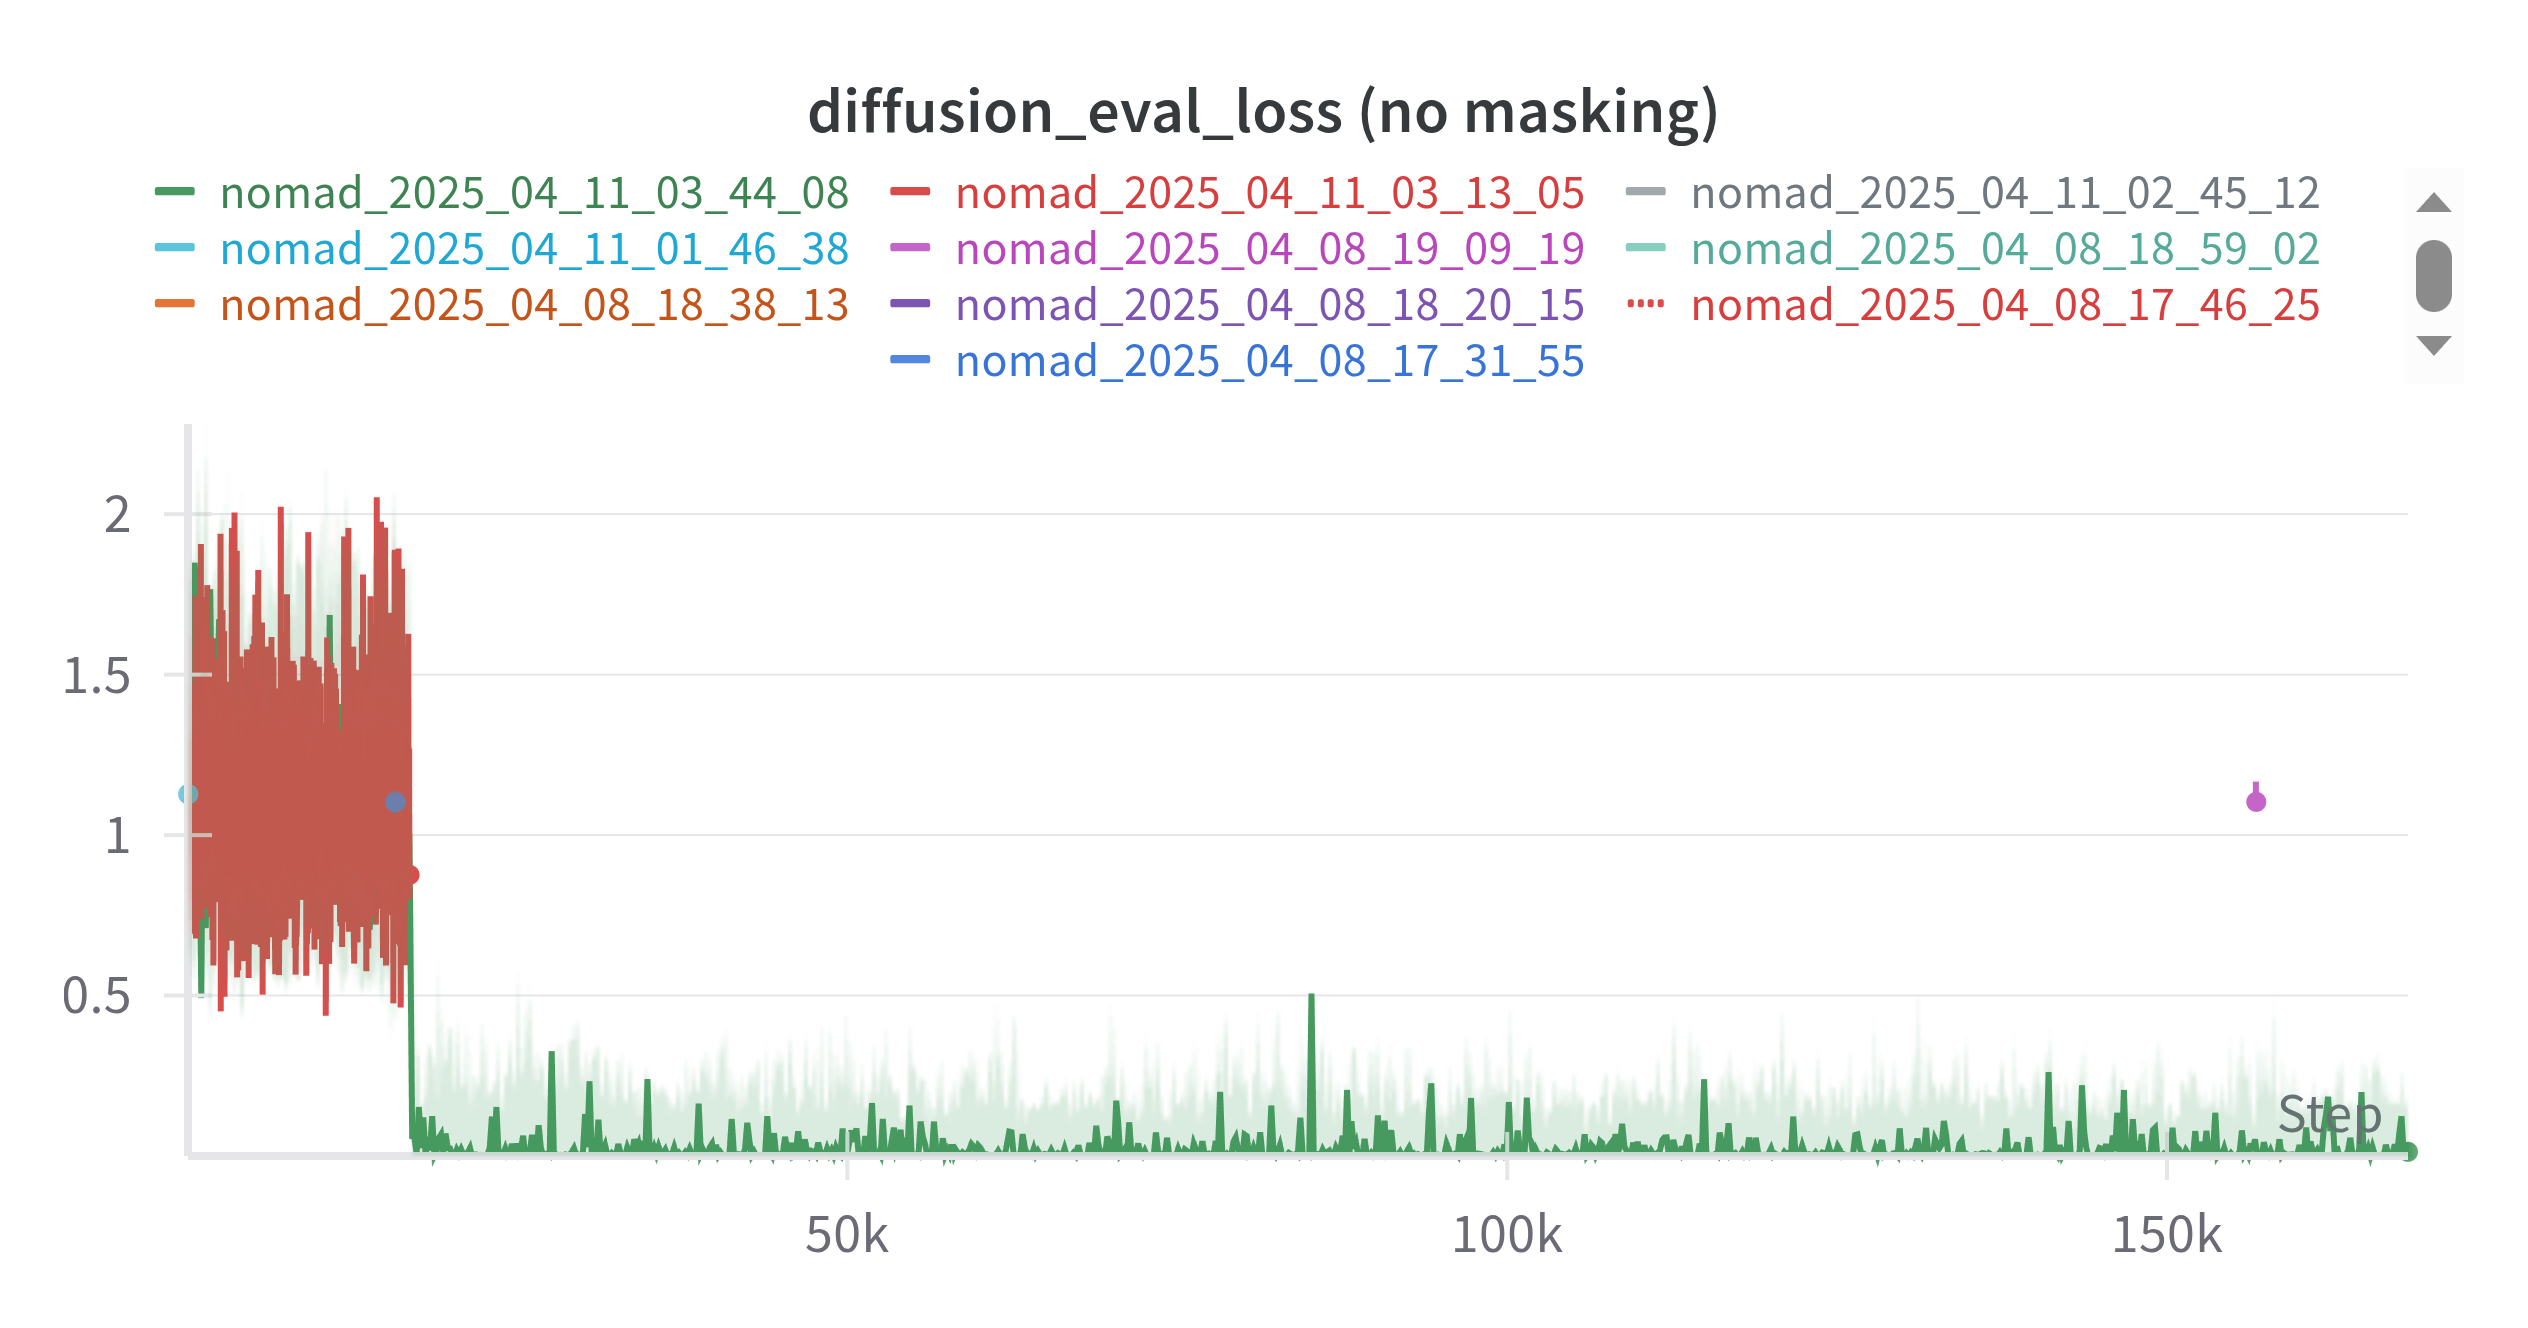
\includegraphics[width=\textwidth]{images/diffusion_eval_loss_no_masking.png}
        \caption{Diffusion evaluation loss without masking}
        \label{fig:diffusion_eval_loss_no_masking}
    \end{subfigure}
    \hfill
    \begin{subfigure}[H]{0.48\textwidth}
        \centering
        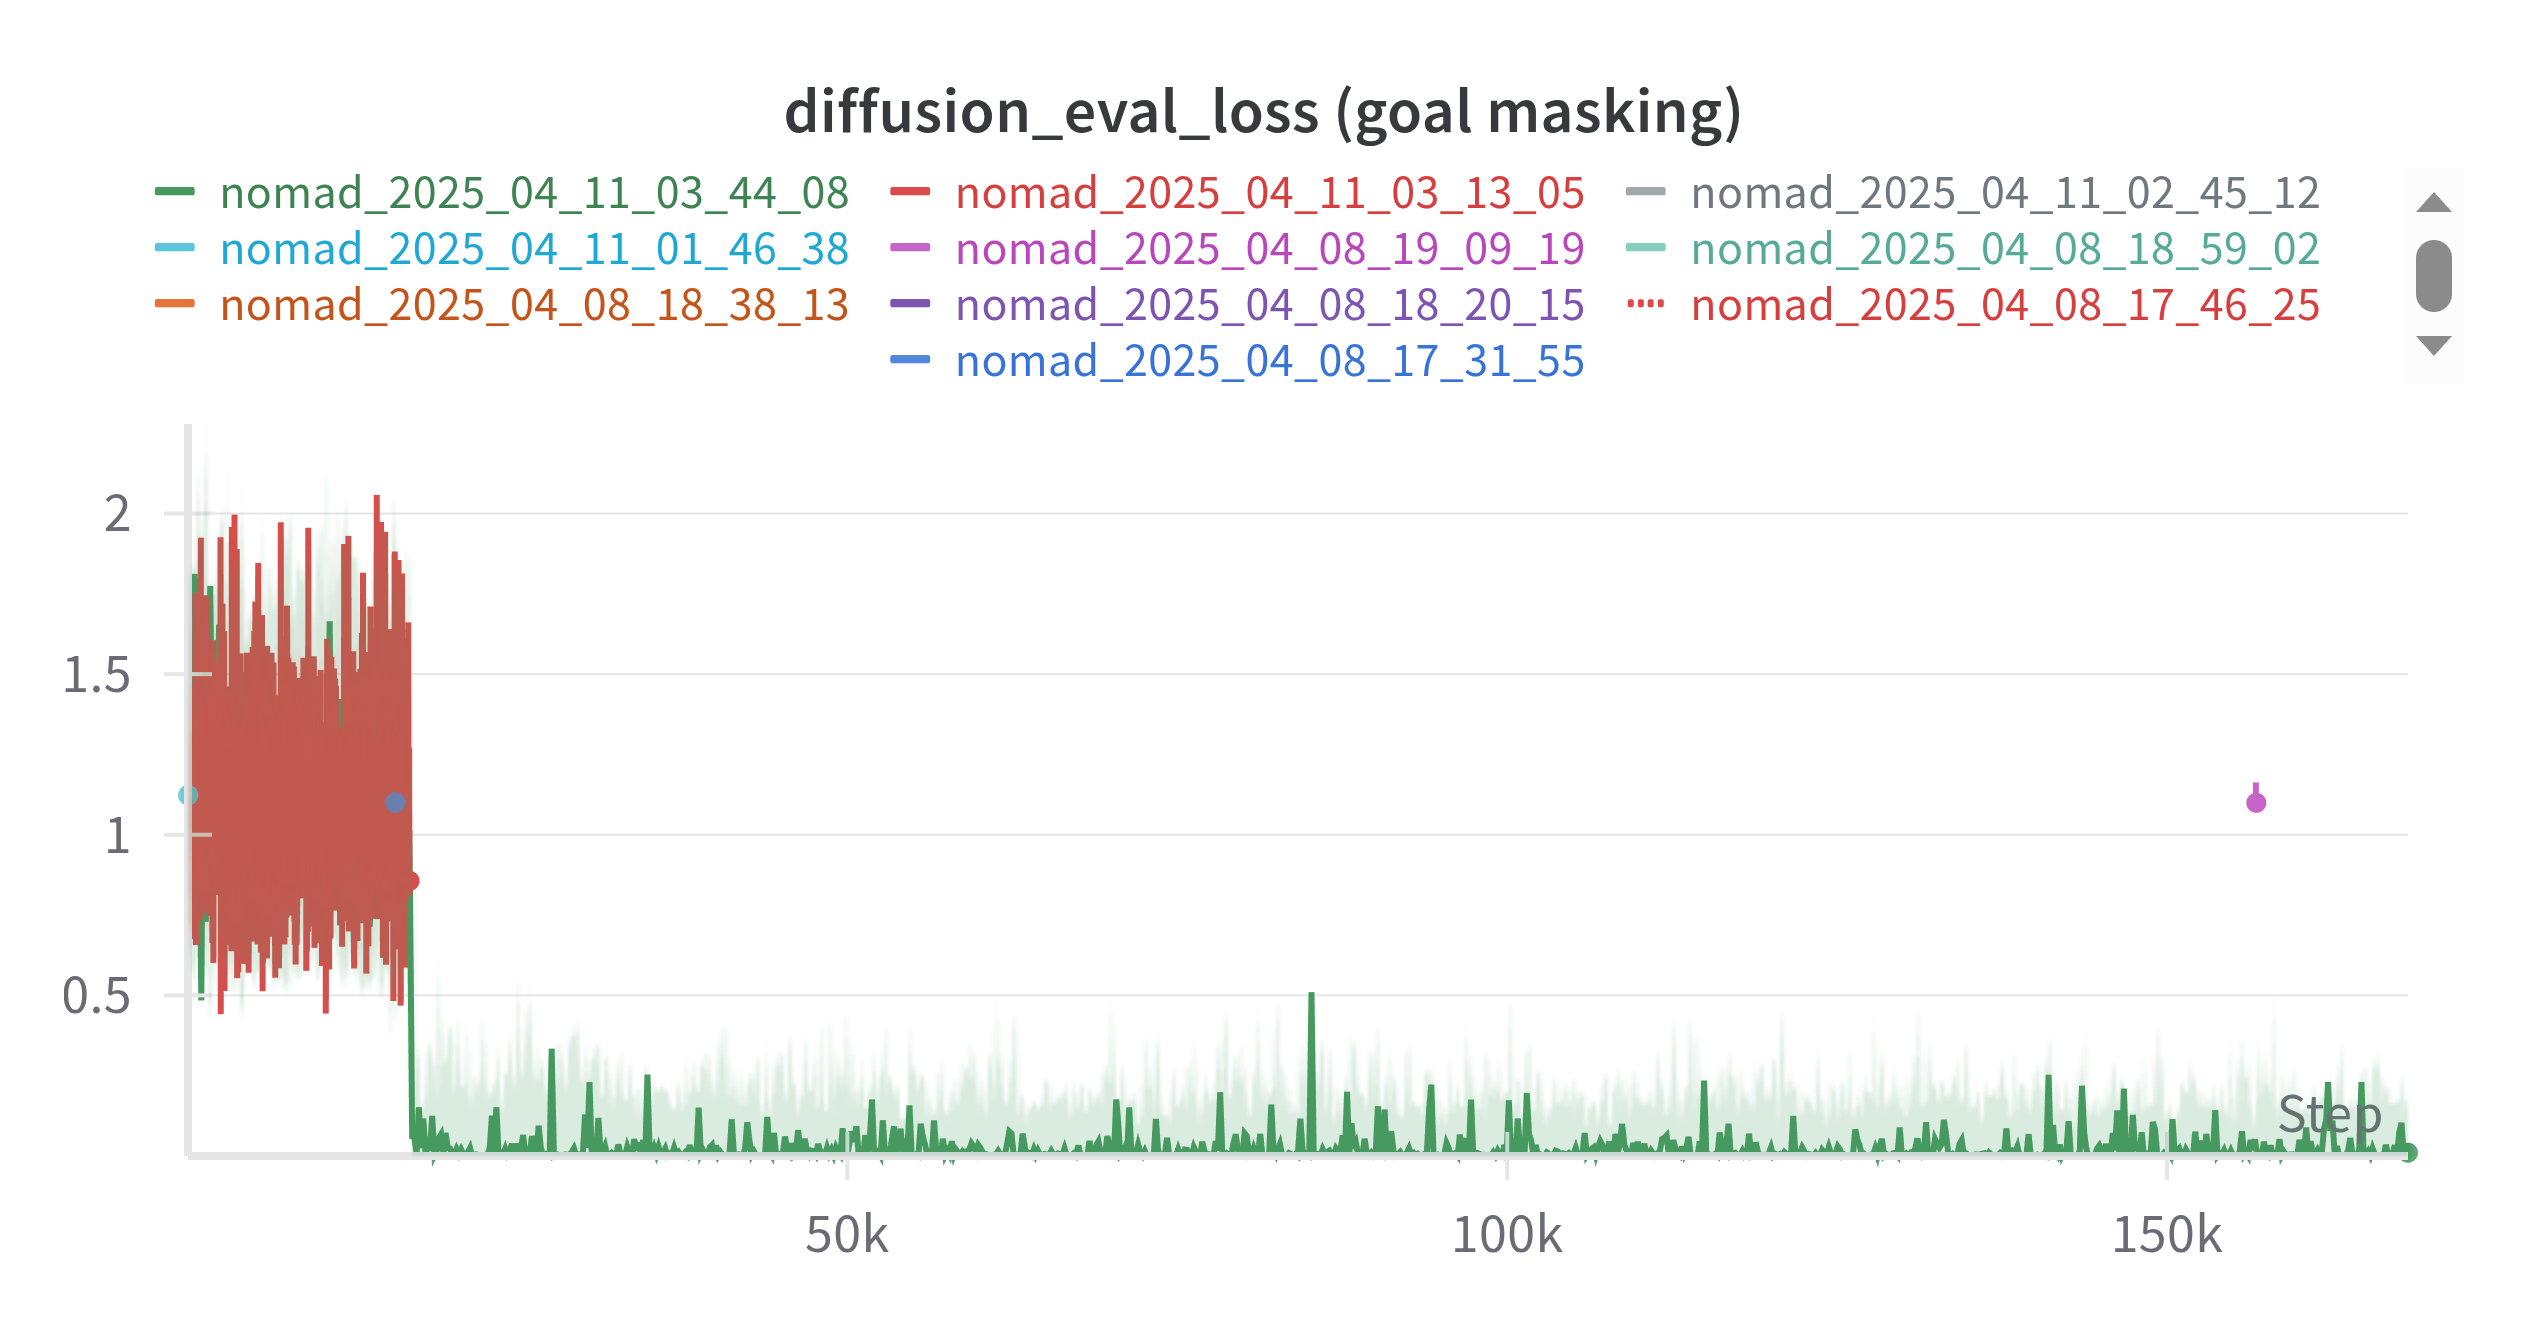
\includegraphics[width=\textwidth]{images/diffusion_eval_loss_goal_masking.png}
        \caption{Diffusion evaluation loss with goal masking}
        \label{fig:diffusion_eval_loss_goal_masking}
    \end{subfigure}
    \caption{Diffusion loss on training set and evaluation loss with different masking strategies}
   \label{fig:diffusion_loss_figure} 
\end{figure}
Figure \ref{fig:diffusion_loss_figure} compares the diffusion loss during training with the evaluation loss under different masking strategies: random masking, no masking, and goal masking.\\
\begin{enumerate}
    \item \ref{fig:diffusion_loss} The diffusion loss starts relatively high and then decreases sharply around the 30k-40k step mark, eventually stabilizing at a much lower level. This suggests that the diffusion model learns effectively during training.
    \item \ref{fig:diffusion_eval_loss_goal_masking}, \ref{fig:diffusion_eval_loss_no_masking} and \ref{fig:diffusion_eval_loss_random_masking} indicate that the evaluation losses (with all masking strategies) are generally higher and more unstable than the training loss. All of the losses drop significantly in the initial evaluation steps.
\end{enumerate}
\newpage
\noindent \textbf{Total Loss:}\\
\begin{figure}[H]
    \centering
    \begin{subfigure}[b]{0.8\textwidth}
        \centering
        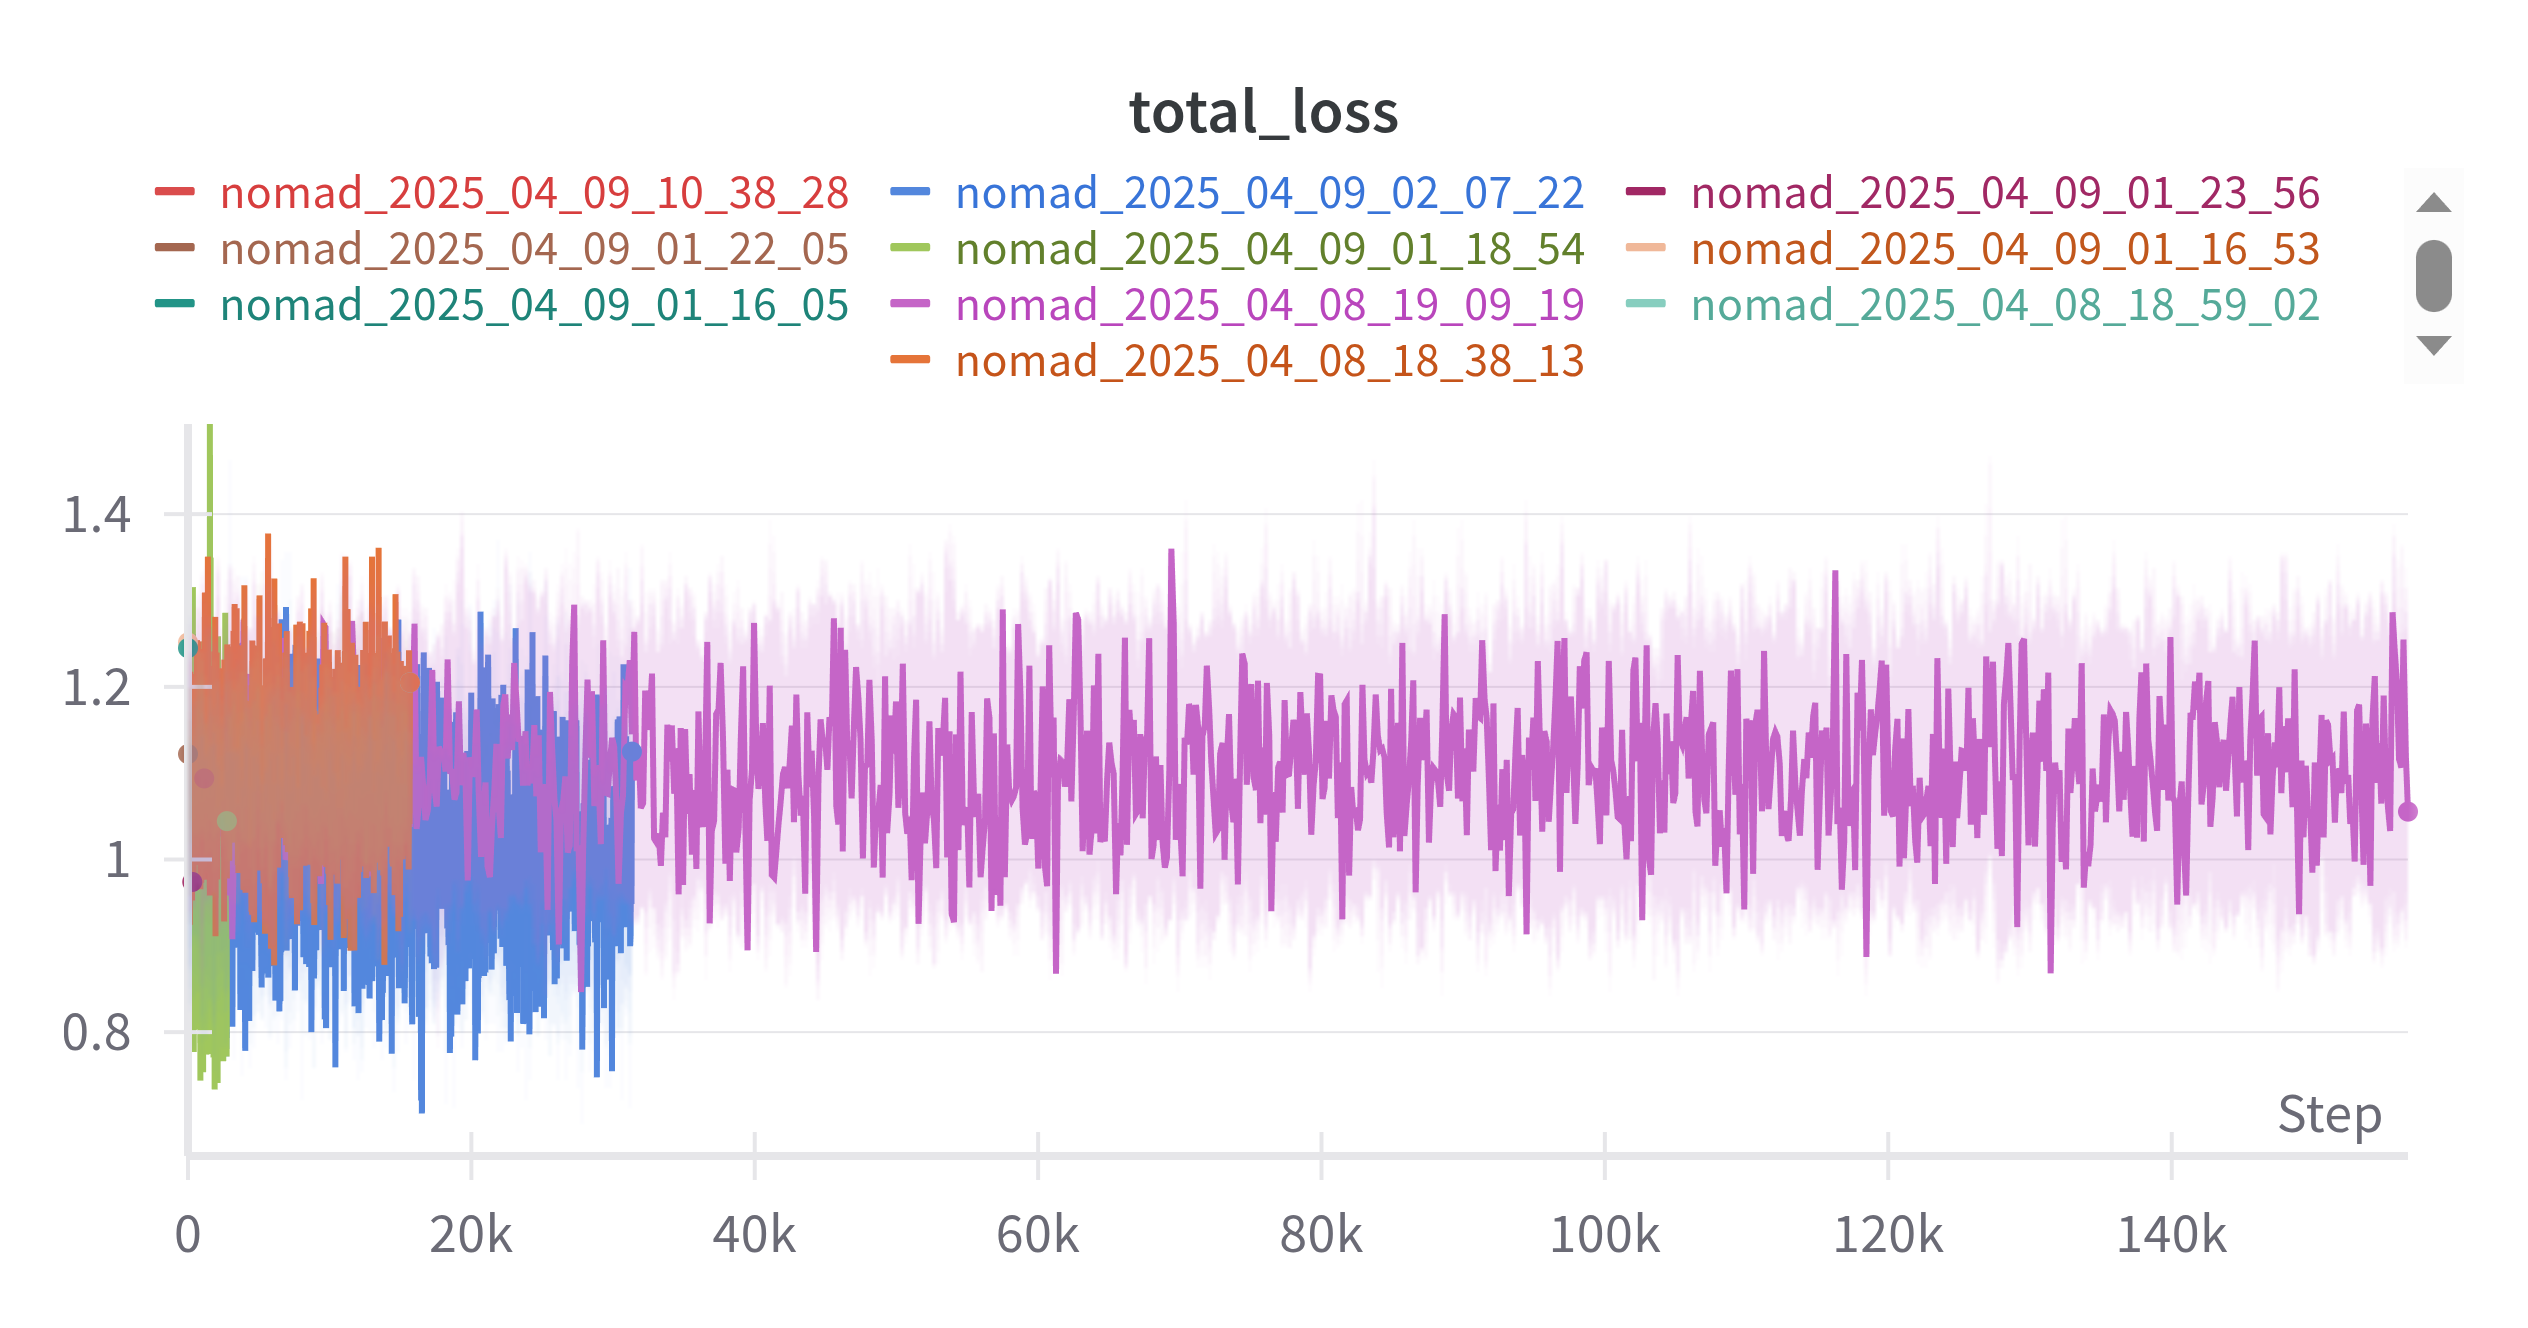
\includegraphics[width=\textwidth]{images/total_loss.png}
        \caption{Total Loss on Training Set}
        \label{fig:total_loss}
    \end{subfigure}
    \end{figure}
The plot agrees that the model is learning effectively, confirmed by the sharp drop in the loss around 35k steps. The model appears to converge to a stable solution.\\

\noindent \textbf{Remarks:}\\
The plots in \ref{fig:dist_loss}, \ref{fig:diffusion_loss} and \ref{fig:total_loss} correspond to another run of the experiment with similar datasets, conditions and parameters.\\
Refer to Appendix \ref{app:wandb} for more details regarding the plots of \texttt{distance\_loss}, \texttt{diffusion\_loss} and \texttt{total\_loss}

\subsection*{Comparison with ViNT}
Both models were evaluated under identical conditions and intrestingly in the \textbf{goal-conditioned (GC)} setting, both demonstrated comparable performances.
Refer to Appendix \ref{app:comparison_vint} for further comparision plots.
\begin{figure}[H]
    \begin{subfigure}[b]{0.48\textwidth}
        \centering
        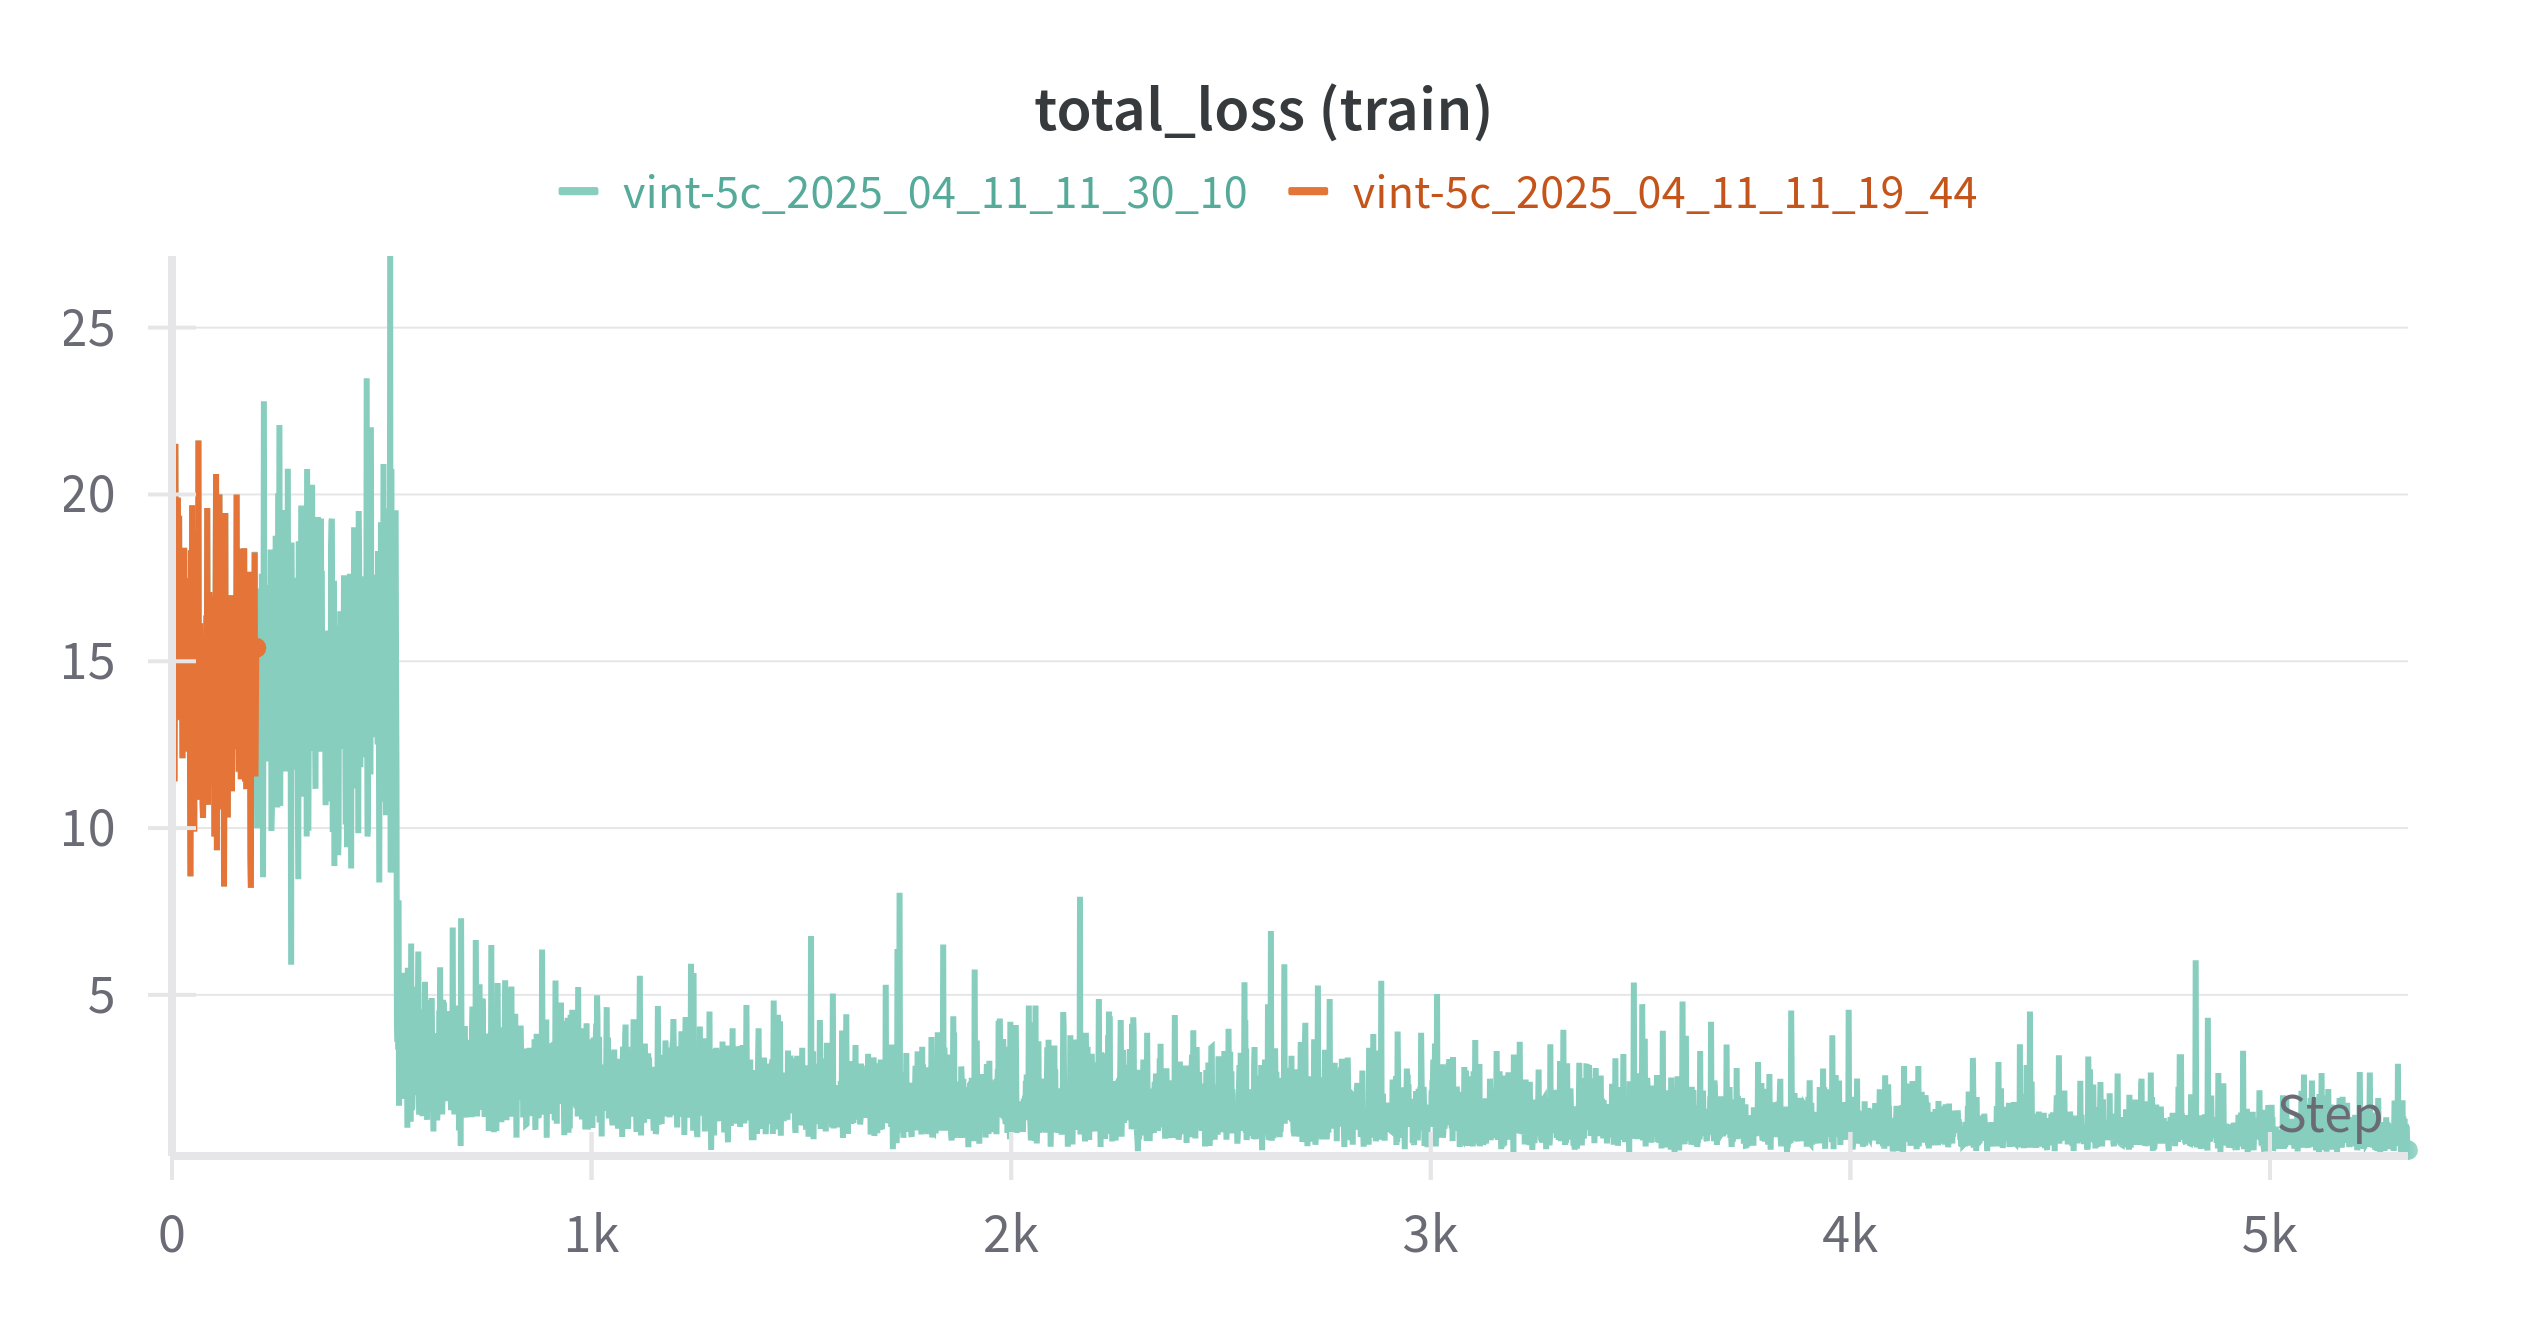
\includegraphics[width=\textwidth]{images/distloss_vint.png}
        \caption{Total Loss on Training Set for ViNT}
    \end{subfigure}
    \hfill
    \begin{subfigure}[b]{0.48\textwidth}
        \centering
        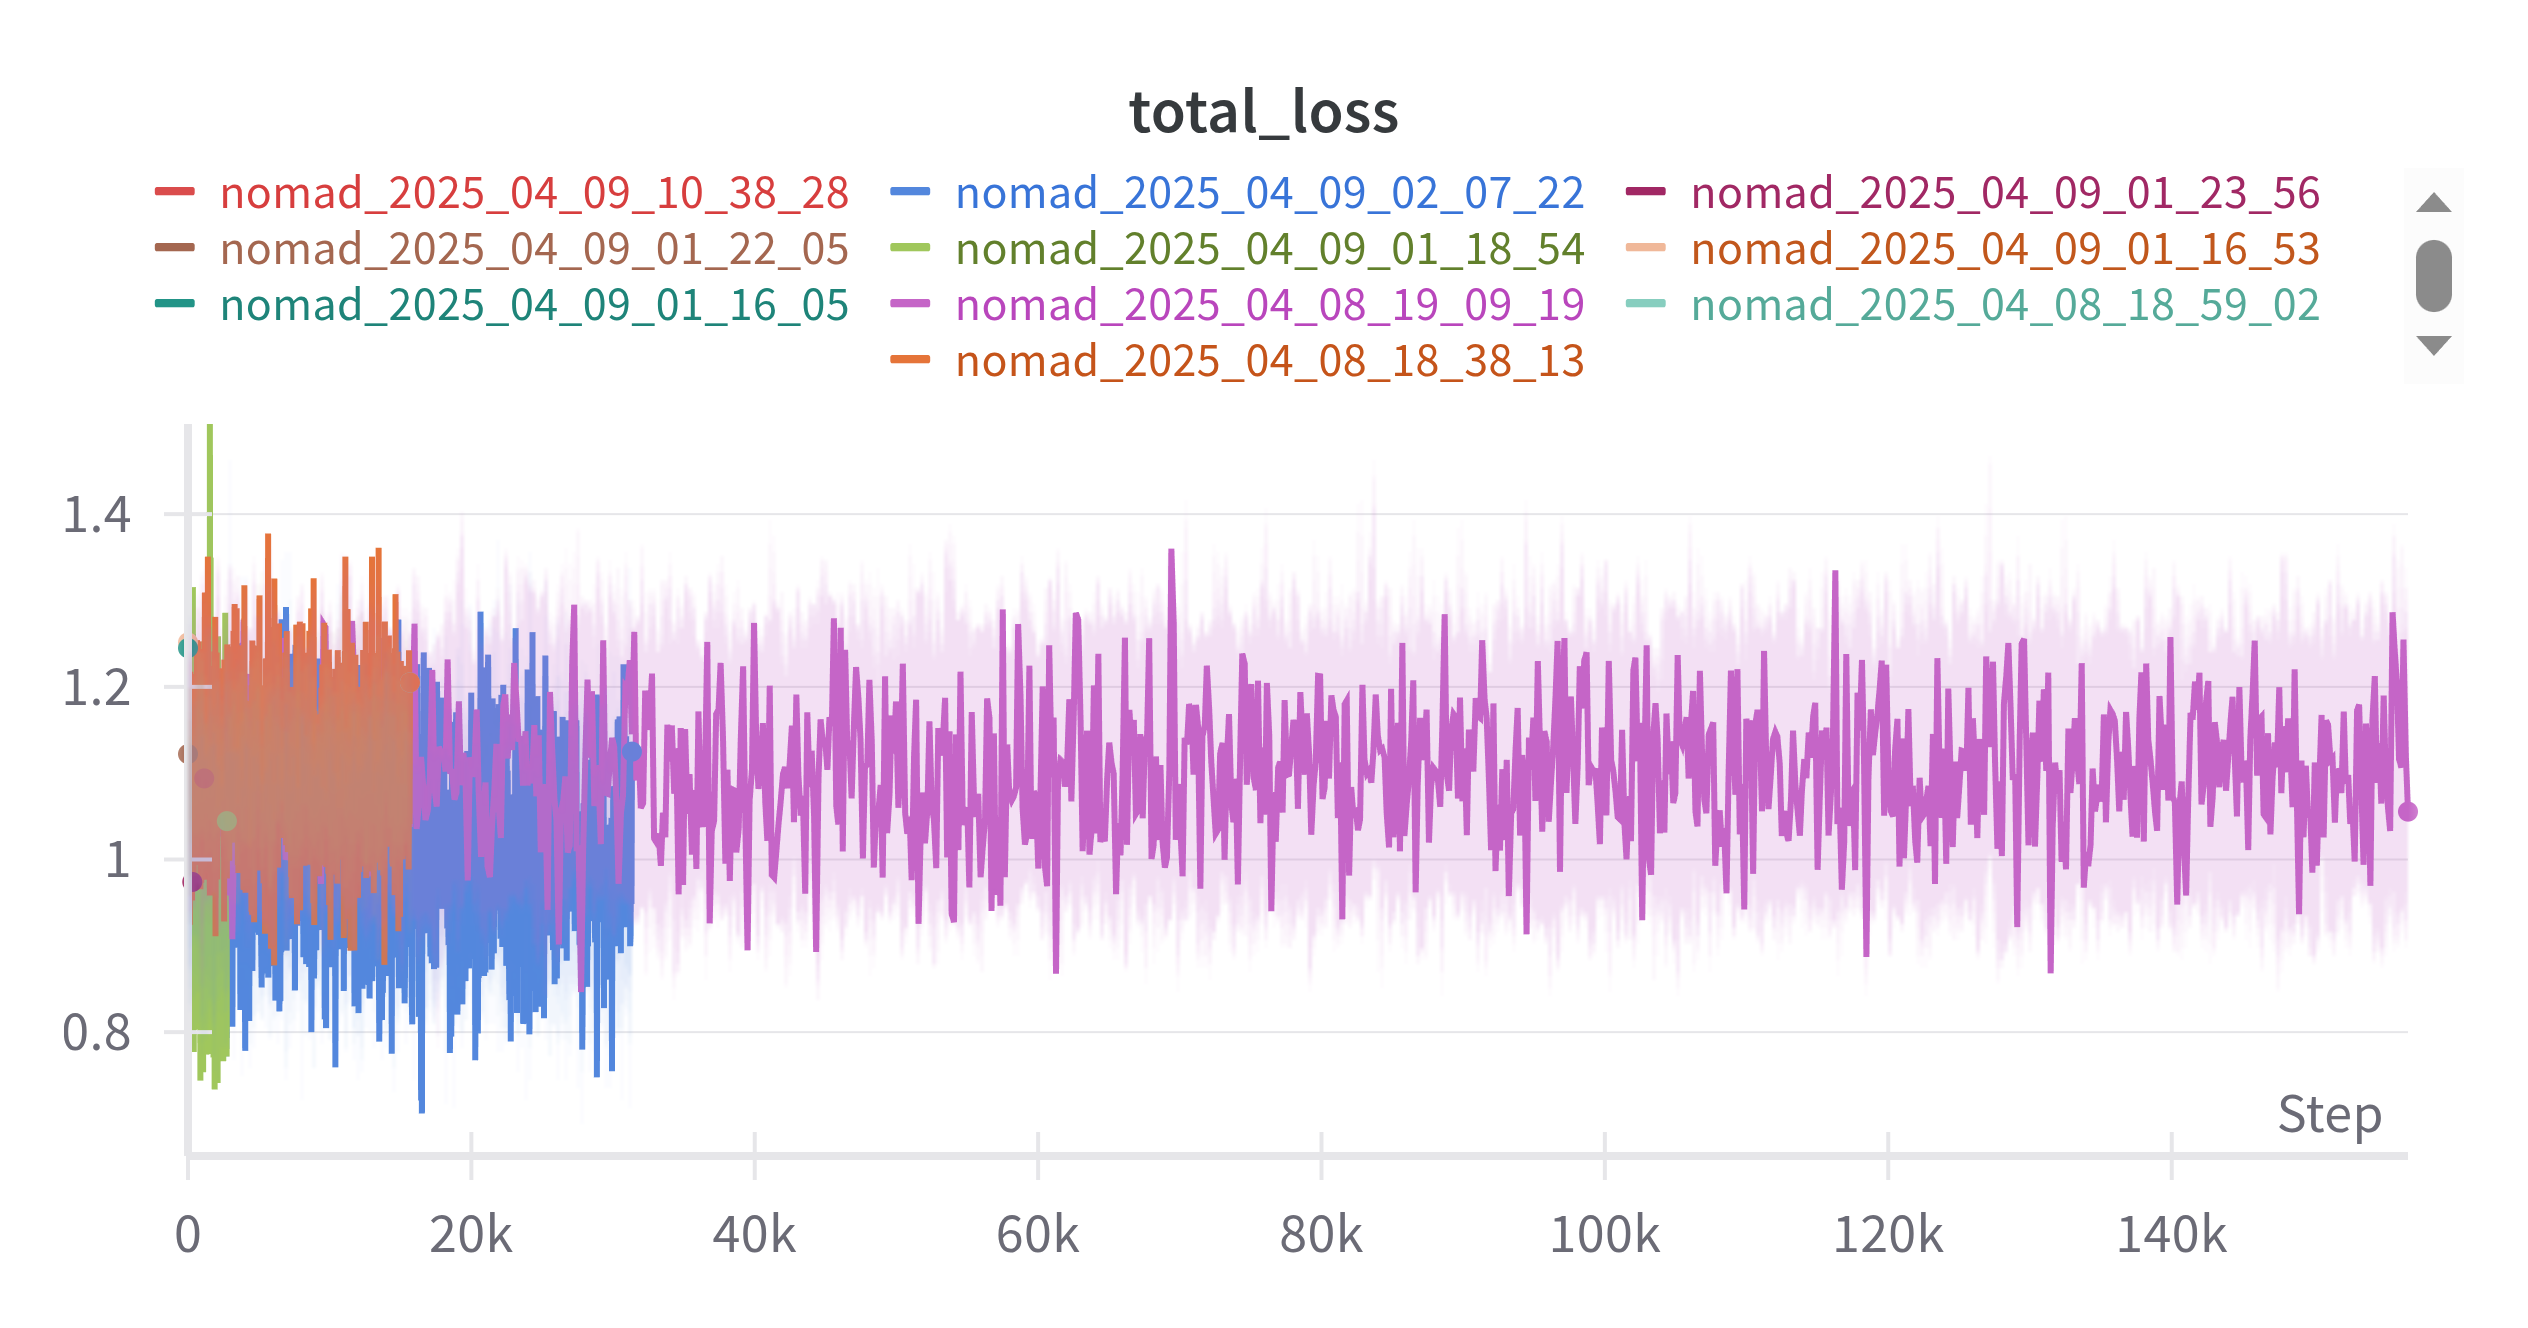
\includegraphics[width=\textwidth]{images/total_loss.png}
        \caption{Total Loss on Training Set for NoMaD}
    \end{subfigure}
\end{figure}
\newpage
\begin{appendices}
\begin{itemize}
    \item \hyperref[app:related_work]{\textbf{Appendix A:}} Related Work and Contextual Foundations of NoMaD
    \item \hyperref[app:preliminaries]{\textbf{Appendix B:}} Technical Preliminaries
    \item \hyperref[app:method_ctd]{\textbf{Appendix C:}} Methodology Ctd.
    \item \hyperref[app:implementation]{\textbf{Appendix D:}} Implementation Details
    \item \hyperref[app:results]{\textbf{Appendix E:}} Results and Experiments
    \item \hyperref[app:comparison_vint]{\textbf{Appendix E:}} Comparison with ViNT
    \item \hyperref[app:app:vit]{\textbf{Appendix F:}} Vision Transformer
    \item \hyperref[app:efficientnet]{\textbf{Appendix G:}} EfficientNet
    \item \hyperref[app:diffusion]{\textbf{Appendix H:}} Diffusion Models
    \item \hyperref[app:wandb]{\textbf{Appendix I:}} Weights and Biases
    \item \hyperref[app:team_contributions]{\textbf{Appendix J:}} Team Contributions
    \item \hyperref[app:challenges]{\textbf{Appendix K:}} Challenges and Debugging
    \item \hyperref[references]{\textbf{References}}
\end{itemize}
\section{Related Work and \\ Contextual Foundations of NoMaD}
\label{app:related_work}
Exploration in unfamiliar enviroments is approached as the problem of efficient mapping, typically formulated around information maximization to guide the robot toward unexplored regions.\\
We factorize the classical exploration problem into two categories:\\
\begin{itemize}
    \item Local exploration strategies that rely on current observations. Objective is to learn control policies that can take diverse,short-horizon actions
    \item Global exploration strategies that utilize a map of the environment. Basically a high-level planner based on a topological graph that uses the policy for long-horizon goal-seeking
\end{itemize}
Robots exploring a new area are essentially trying to map it efficiently—this means covering as much area as possible, ideally without wasting time.\\
However, building detailed geometric maps, can be difficult without accurate depth perception. \\
Several prior approaches have investigated learning-based exploration policies. Some approaches use simulation data (training in virtual environments).\\
Others learn from real-world data directly. These models may use:\\
\begin{itemize}
    \item Intrinsic rewards: Encouraging the robot to explore new things.
    \item Semantic prediction: Going to interesting or informative places.
    \item Latent variable models: Abstract models of how actions affect the world.
\end{itemize}
Yet, policies trained in simulation frequently struggle to transfer to real-world environments. Even real-world-trained models can underperform in complex indoor and outdoor settings.\\
\bigskip
\noindent \textbf{Enter NoMaD : A New Method}\\ 
The work most closely related to NoMaD is ViNT (refer Appendix X for more details), which combines a goal-conditioned policy with a separate subgoal proposal module. The subgoal proposals are generated using an image diffusion model, condiitioned on robot's current view.\\
NoMaD improves on this by:
\begin{itemize}
    \item Not generating images.
    \item Directly predicting actions using diffusion models, which are typically used in image generation tasks but can model complex probabilities really well.
    \item This makes NoMaD more accurate and much lighter (needs 15x fewer parameters).
\end{itemize}
One of the core challenges in modeling robot exploration policies is the inherently multimodal nature of action sequences.\\
Observation-conditioned diffusion models  have emerged as powerful tools because they can learn complex action distributions without needing without needing explicit state prediction.\\
Nomad builds upon this adding \textbf{goal conditioning} to diffusion-based action generation, meaning it is capable of both:
\begin{itemize}
    \item Goal-directed exploration
    \item Undirected exploration 
\end{itemize}

\section{Technical Preliminaries}
\label{app:preliminaries}
The primary objective is to develop a visual navigation policy, denoted by $\pi$, that enables a robot to navigate using only RGB images from its onboard camera. \\
The policy devised should operates as follows:
\begin{itemize} 
    \item It receives a sequence of past and current observations: $o_t := o_{t-P : t}$. 
    \item It predicts a distribution over future actions: $a_t := a_{t : t+H}$. 
    \item Optionally, it can also condition on a goal image $o_g$, representing the desired destination. 
\end{itemize}
Depending on whether a goal is provided, the policy behaves differently: 
\begin{itemize} 
    \item \textbf{Goal-directed navigation:} When a goal image $o_g$ is available, $\pi$ generates actions that guide the robot toward the goal. 
    \item \textbf{Exploratory behavior:} When no goal is given (as in pure exploration settings), $\pi$ must still generate safe and purposeful actions—avoiding obstacles and staying on traversable paths—while efficiently covering the environment. 
\end{itemize}
To handle long-horizon planning and complex environments, the system is further augmented with: 
\begin{itemize} 
    \item A topological memory graph $\mathcal{M}$, which maintains a structured map of past visual observations. 
    \item A high-level planner that leverages this memory to decide on intermediate goals and broader exploration strategies. 
\end{itemize}
\subsection*{Visual Goal-Conditioned Policies: ViNT as the Backbone}
NoMaD builds on the ViNT (Visual Navigation Transformer) architecture, a Transformer-based model tailored for goal-conditioned navigation.\\
\paragraph{Key Components of ViNT:} 
\begin{itemize} 
    \item \textbf{Visual Encoding:} Each observation is processed using an EfficientNet-B0 encoder to extract feature embeddings. 
    \item \textbf{Goal Fusion:} The current and goal image features are combined using a goal fusion encoder. 
    \item \textbf{Transformer Attention:} These fused features (tokens) are passed through a Transformer model to generate a context vector $c_t$. 
    \item \textbf{Predictions:} The context vector is used to predict: 
    \begin{itemize} 
        \item A distribution over future actions: $a_t = f_a(c_t)$. 
        \item An estimate of temporal distance to the goal: $d(o_t, o_g) = f_d(c_t)$. 
    \end{itemize} 
\end{itemize}
These outputs are learned via supervised training, where the model is shown expert trajectories and learns to imitate them.
\begin{quote}
    \textit{However, ViNT is inherently goal-conditioned—it cannot operate in the absence of a goal image, limiting its ability to explore autonomously.} 
\end{quote}
\subsection*{Extending to Long-Horizon Planning with Topological Memory}
To overcome this limitation, NoMaD incorporates a topological memory $\mathcal{M}$: 
\begin{itemize} 
    \item Nodes represent previously encountered visual observations. 
    \item Edges represent traversable paths, established using ViNT's predicted distances. 
\end{itemize}
This memory graph enables both: 
\begin{itemize} 
    \item \textbf{Subgoal Planning:} If a goal cannot be reached directly, the planner identifies a sequence of reachable subgoals via $\mathcal{M}$. 
    \item \textbf{Structured Exploration:} Even without a goal, $\mathcal{M}$ helps guide exploration toward promising, yet-unvisited areas. 
\end{itemize}
\subsection*{Frontier-Based Exploration with NoMaD}
To evaluate NoMaD's ability to generalize to new environments, the authors implement a frontier-based exploration strategy:
\begin{itemize} 
    \item \textbf{Frontier:} The boundary between explored and unexplored areas in the environment. 
    \item The high-level planner selects frontiers as subgoals, encouraging the robot to expand coverage. 
\end{itemize}
This builds on the ViKiNG framework, but replaces its prior policy with NoMaD, which supports both: 
\begin{itemize} 
    \item \textbf{Goal-seeking} behavior (when a goal image is provided), and 
    \item \textbf{Autonomous exploration} (when no goal is available). 
\end{itemize}

\section{Methodology: Ctd.}
\label{app:method_ctd}
\subsection*{Architecture Overview}
\label{subsec:architecture}
Figure \ref{fig:nomad_architecture} illustrates the NoMaD architecture, which consists of three main components:

\begin{figure}[H]
    \centering
    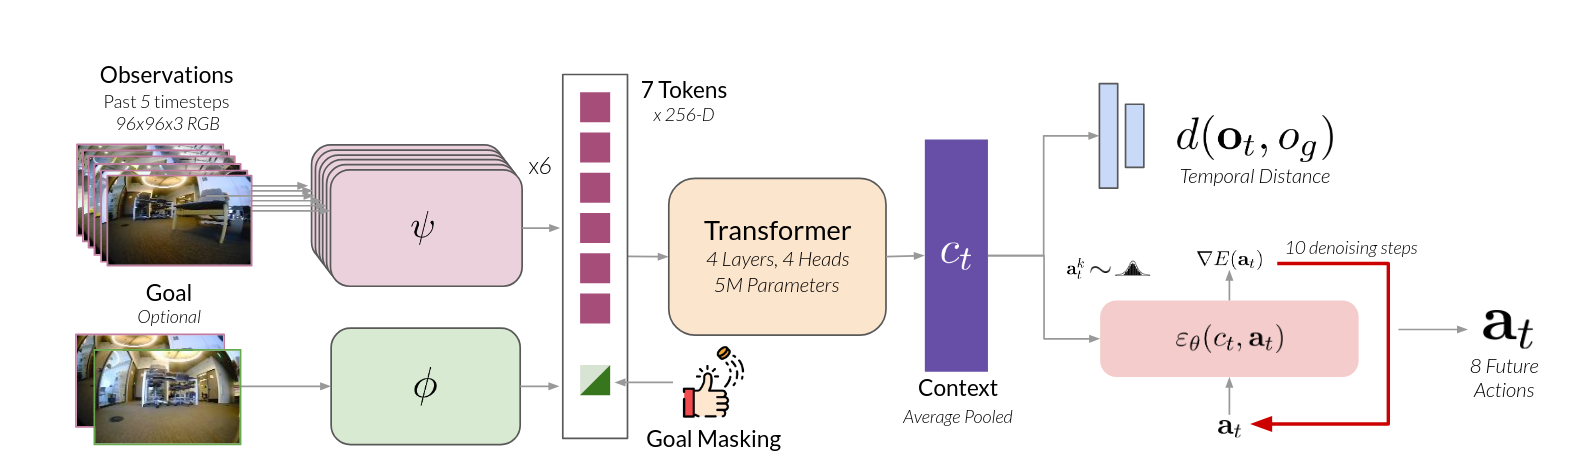
\includegraphics[width=0.85\textwidth]{nomad_diagram.png}
    \caption{NoMaD architecture. The visual encoder processes RGB observations, the transformer maintains temporal context, and the diffusion decoder generates waypoint predictions. Goal masking occurs in the attention layers of the context encoder.}
    \label{fig:nomad_architecture}
\end{figure}


\subsection*{A. Attention based Goal Masking}
\label{subsec:goal_masking}
To seamlessly switch between goal-directed behavior and exploration, we set a binary goal mask m in NoMaD.
The model builds on the ViNT (Visual Navigation Transformer) framework, by modifying the the computation of the observation context vector $c_t$ as follows:\\
\[
c_t = f(\psi(o_i), \phi(o_t, o_g), m)
\]
where:
\begin{itemize}
    \item $\psi(o_i)$: Encodes the current observation.
    \item $\phi(o_t, o_g)$: Encodes the time-step and goal image.
    \item $m$: A binary mask that determines whether to attend to the goal image or not.
\end{itemize}
\begin{itemize}
    \item When $m = 0$, the policy \textbf{attends to the goal image} $o_g$ to perform goal-conditioned navigation.
    \item When $m = 1$, the goal pathway is \textbf{masked out}, resulting in undirected exploration. Masking is applied in the attention layers, so goal embeddings are ignored if m=1.
\end{itemize}
During training, the goal mask $m$ is sampled from a Bernoulli distribution with probability $p_m = 0.5$, ensuring equal exposure to both behaviors. \\
At test time, $m$ is explicitly set based on the task: $m = 0$ for goal-reaching, and $m = 1$ for exploration.

\subsection*{B. Diffusion Policy}
Refer to Appendix \ref{app:diffusion} for more on Diffusion policies.\\
In general, diffusion models are generative models that work by gradually adding noise to data (a forward process), and then learning to remove that noise (a reverse denoising process) to generate realistic samples.\\
To model complex, multimodal action distributions, especially in unstructured or ambiguous environments, NoMaD employs a \textbf{diffusion model} to approximate the conditional distribution of the next action as $p(a_t | c_t)$. \\
The denoising process is as follows:\\
1. \textbf{Forward Process:} Start with a real action $a^{0}_t$ from the dataset and add gaussian noise over multiple steps (K). 
\begin{center}
    $a^{k}_t = \sqrt{\alpha_k} a^{k-1}_t + (\sqrt{1 - \alpha_k}) \epsilon$
\end{center}
where:\\
\begin{itemize}
    \item $\epsilon$ $\sim$ $\mathcal{N}$(0,I) is a random noise
    \item $\alpha_k$ is a noise scheduler (eg square cosine)
    \item By step K, the action is almost pure noise.
\end{itemize}
2. \textbf{Reverse Denoising(Learned Model):} starting from pure noise $a^{k}_t$ $\sim$ $\mathcal{N}(0,I)$, it denoises step by step to recover the final clean action $a^{0}_t$.\\
Each denoising step is :
\begin{center}
    \[a^{k-1}_t = \alpha(\alpha^{k}_t-\gamma_k.\epsilon_{\theta}(c_t, a^{k}_t,k)) + \mathcal{N}(0,\sigma^2.I)\]
\end{center}
Where:
\begin{itemize}
    \item Here, $\epsilon_\theta$ is the noise prediction network conditioned on the context $c_t$, which may or may not include the goal depending on $m$.
    \begin{itemize}
        \item It is a 1D conditional U-Net with 15 CNN layers.
        \item Input:the noisy action $a^{k}_t$, the context vector $c_t$, and the diffusion step k.
        \item the predicted noise vector $\hat{\epsilon}_k$,During training, it is compared to the true noise added earlier.
    \end{itemize}
    \item $\gamma, \alpha ,\sigma$ are scheduler constants.
\end{itemize}

\section{Implementation Details}
\label{app:implementation}
\subsection{Environment Setup}
All experiments were conducted on a system equipped with an NVIDIA GeForce GTX 1660 SUPER GPU and a 12\textsuperscript{th} Gen Intel\textregistered~Core\texttrademark~i9-12900K (24-core) processor. \\
The code was implemented in Python 3.12.9 in a conda environment. All the packages and libraries used are listed in the requirements.txt file in the github repo.\\
The codebase was adapted from an open-source repository\cite{gitnomad}, and experiment tracking was performed using \texttt{Weights \& Biases (WandB)} for logging loss curves, evaluation metrics, and debugging errors. Refer to Appendix \ref{app:wandb} for more details and results.\\
\subsection{Data Pipeline}
We trained the NoMaD model using the \textbf{SACSON} and parts of \textbf{RECON} dataset along with \textbf{go\_stanford}, which contains diverse real-world trajectories across various environments and robot platforms.
The SACSON and go\_stanford dataset were already processed and we it split into training and validation sets using 80-20 split ratio. The RECON dataset consisted of bag files, which needed to be preprocessed to extract RGB images, actions, and ground-truth waypoints.

\textbf{Training Configuration:}
 \begin{itemize}
     \item We trained the model with batch size of 47 for 10 epochs.
     \item The weighting factor $\lambda$ for the auxiliary distance loss was set to $10^{-4}$.
     \item The model was trained using the \textbf{AdamW} optimizer with a learning rate of $1\text{e}^{-4}$ and a weight decay of $1\text{e}^{-2}$.
        \begin{figure}[H]
            \centering
            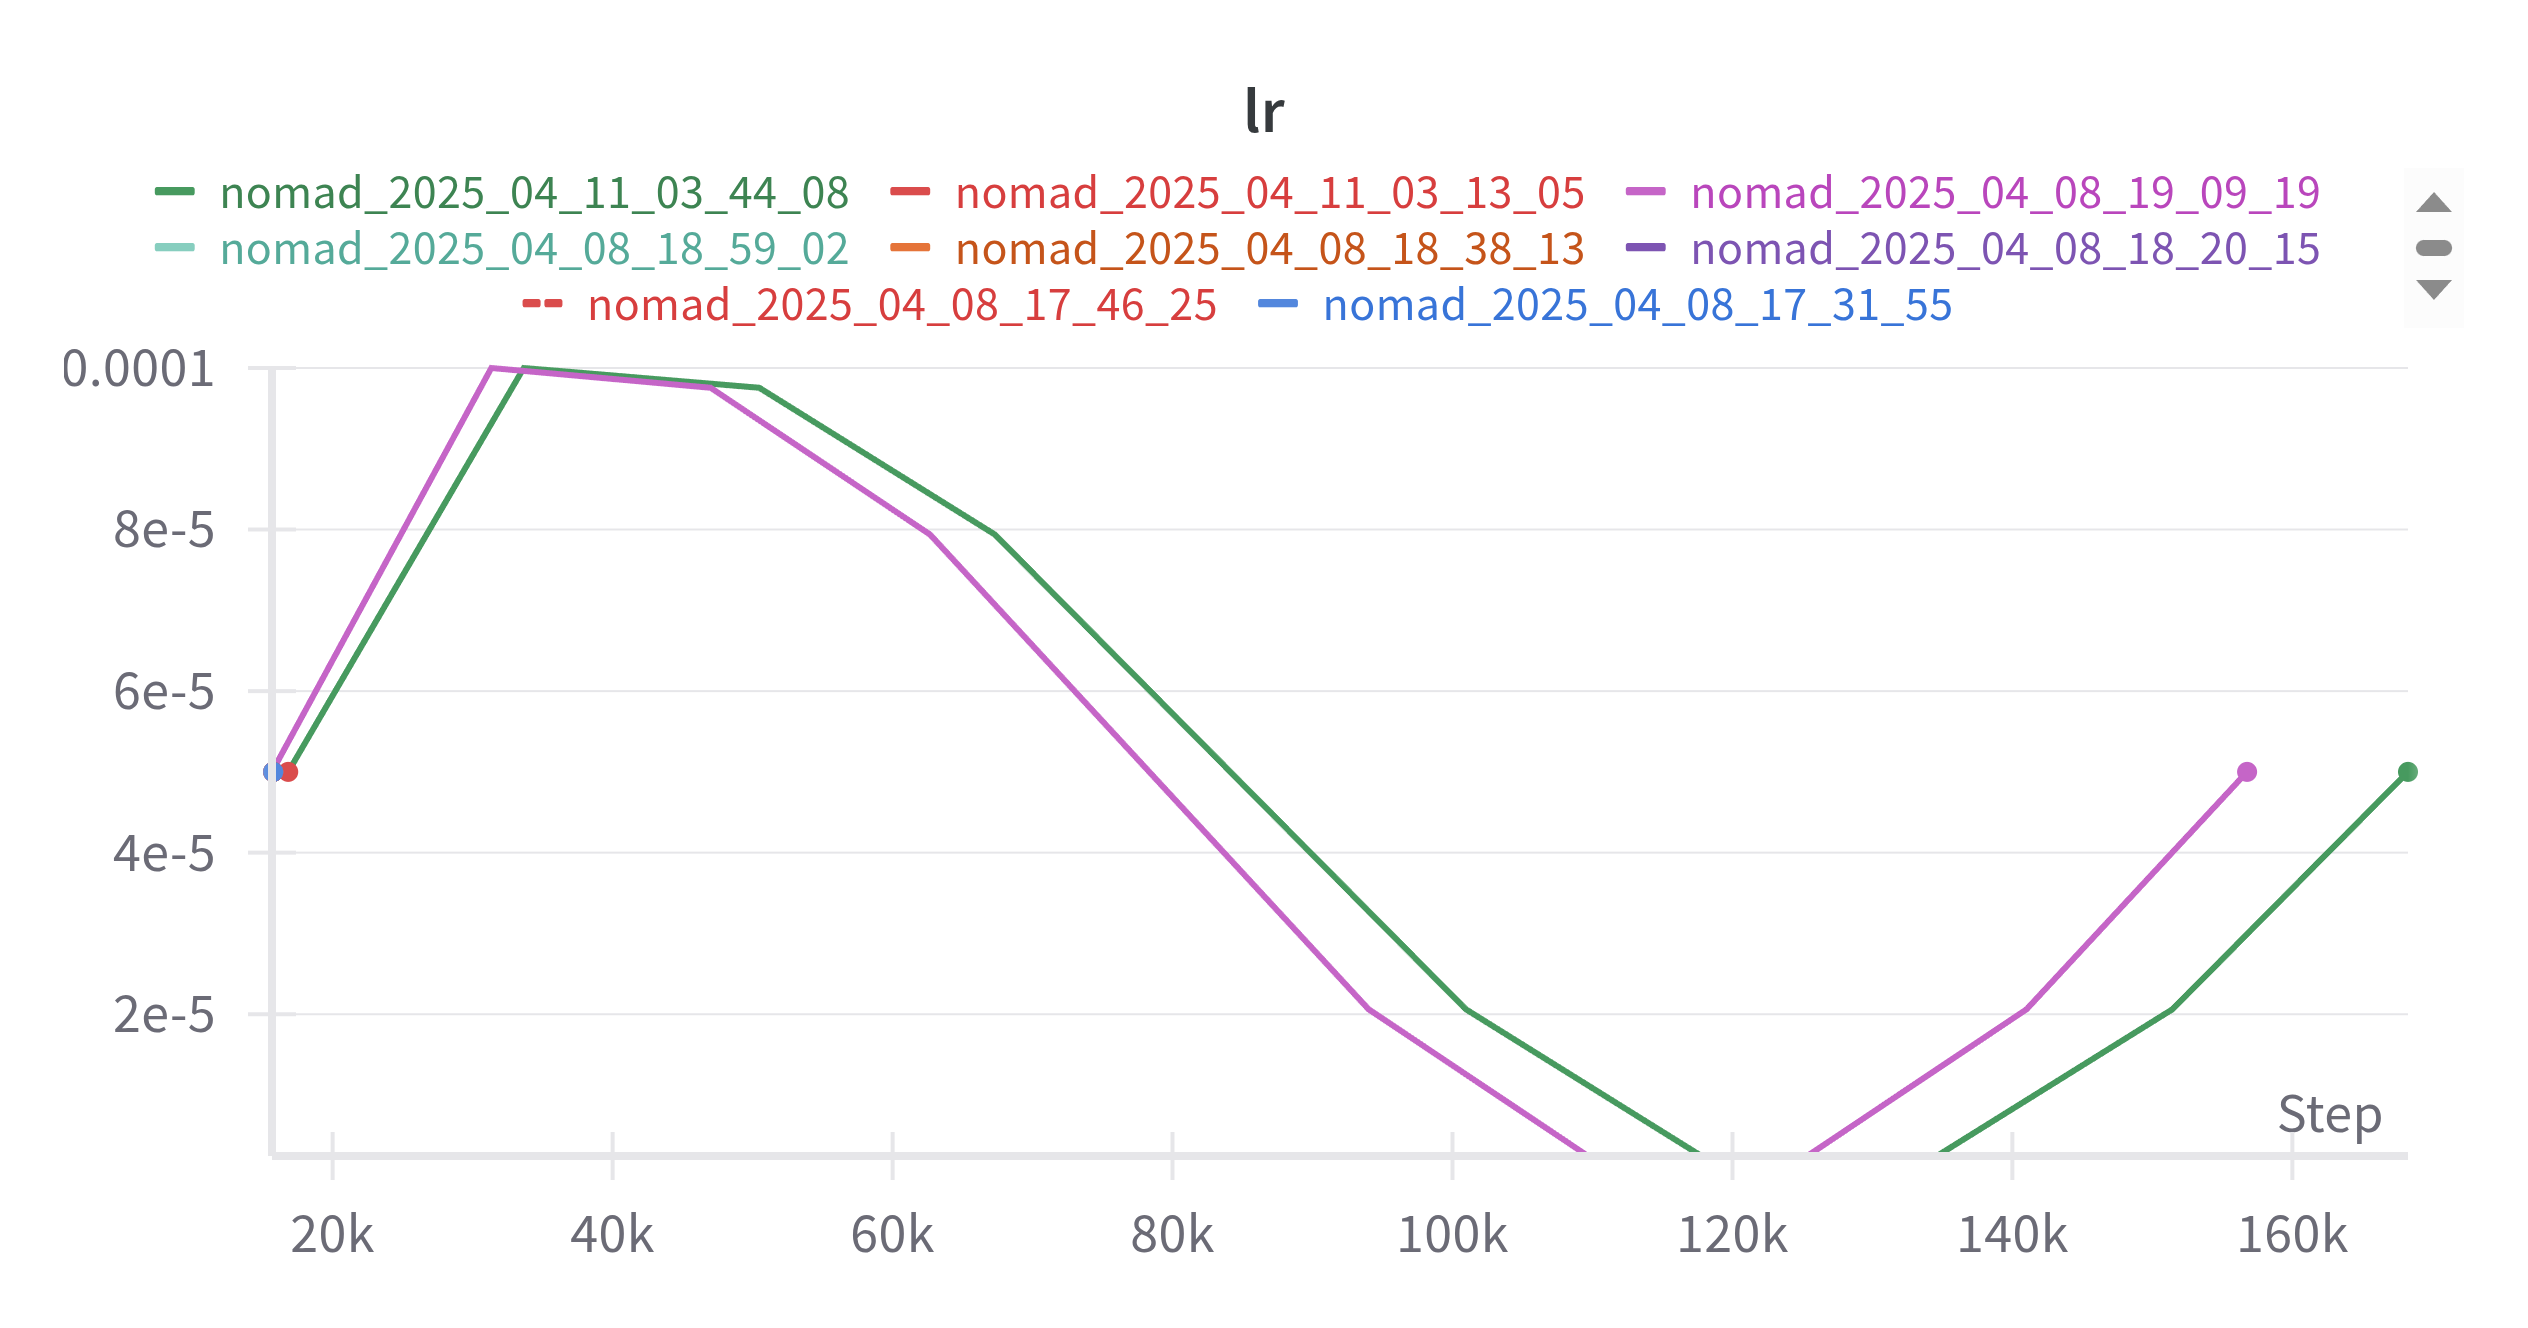
\includegraphics[width=1\textwidth]{images/lr.png}
            \caption{Learned rate schedule for the NoMaD model.}
            \label{fig:lr}
        \end{figure}
     \item We applied \textbf{cosine annealing} to decay the learning rate over time.
     \item We used \textbf{goal masking} with probability $p_m = 0.5$, encouraging the model to generalize across goal-visible and goal-agnostic contexts.
     \item The diffusion process used a \textbf{square cosine schedule} with $K = 10$ denoising steps.
     \item The ViNT observation encoder was an EfficientNet-B0, mapping $96 \times 96$ RGB images into a 256-dimensional latent embedding.
     \item The transformer used for context encoding had 4 layers and 4 attention heads.
     \item Training checkpoints and EMA snapshots were saved at the end of each epoch for model tracking and potential evaluation.
     \item Training and validation loss curves were logged using \texttt{Wandb} for detailed inspection.
\end{itemize}

\noindent \textbf{Evaluation:}\\
Evaluation was performed on the validation set using the following metrics:
\begin{itemize}
    \item distance loss
    \item diffusion loss
    \item cosine similarity
    \item action loss
\end{itemize}

\subsection{Using WandB}
We used wandb to log training progress, visualize losses, and monitor both model behavior and system resources (e.g., GPU/CPU utilization)
throughout experimentation. \\
Metrics such as action loss, goal prediction error, and the learning rate schedule were automatically tracked and visualized, which helped with debugging and plotting out results.
Refer to \hyperref[app:wandb]{Appendix F} for other resulting plots and visualizations.\\

\section{Comparison with ViNT}
\label{app:comparison_vint}
To establish a baseline, we trained the original ViNT architecture using the same dataset and training hyperparameters as used for NoMaD. The model configuration included the same EfficientNet-B0 encoder and transformer-based architecture, but excluded the diffusion decoder.\\

Both models were evaluated under identical conditions on the validation set, using metrics such as Mean Squared Error (MSE) for actions and cosine similarity between predicted and ground-truth waypoints. The ViNT model was trained for 10 epochs with a batch size of 47.\\

Interestingly, in the \textbf{goal-conditioned (GC)} setting, both ViNT and NoMaD demonstrated comparable performance across the key evaluation metrics. This suggests that the integration of a diffusion-based decoder in NoMaD does not negatively impact performance on goal-directed planning tasks. Instead, it enables a more expressive generative modeling capability while preserving task effectiveness.\\

Here are some plots from WandB comparing the two models on the basis of \texttt{distance\_loss} and \texttt{action\_loss}:\\
\begin{figure}[H]
    \centering
    \begin{subfigure}[b]{0.48\textwidth}
        \centering
        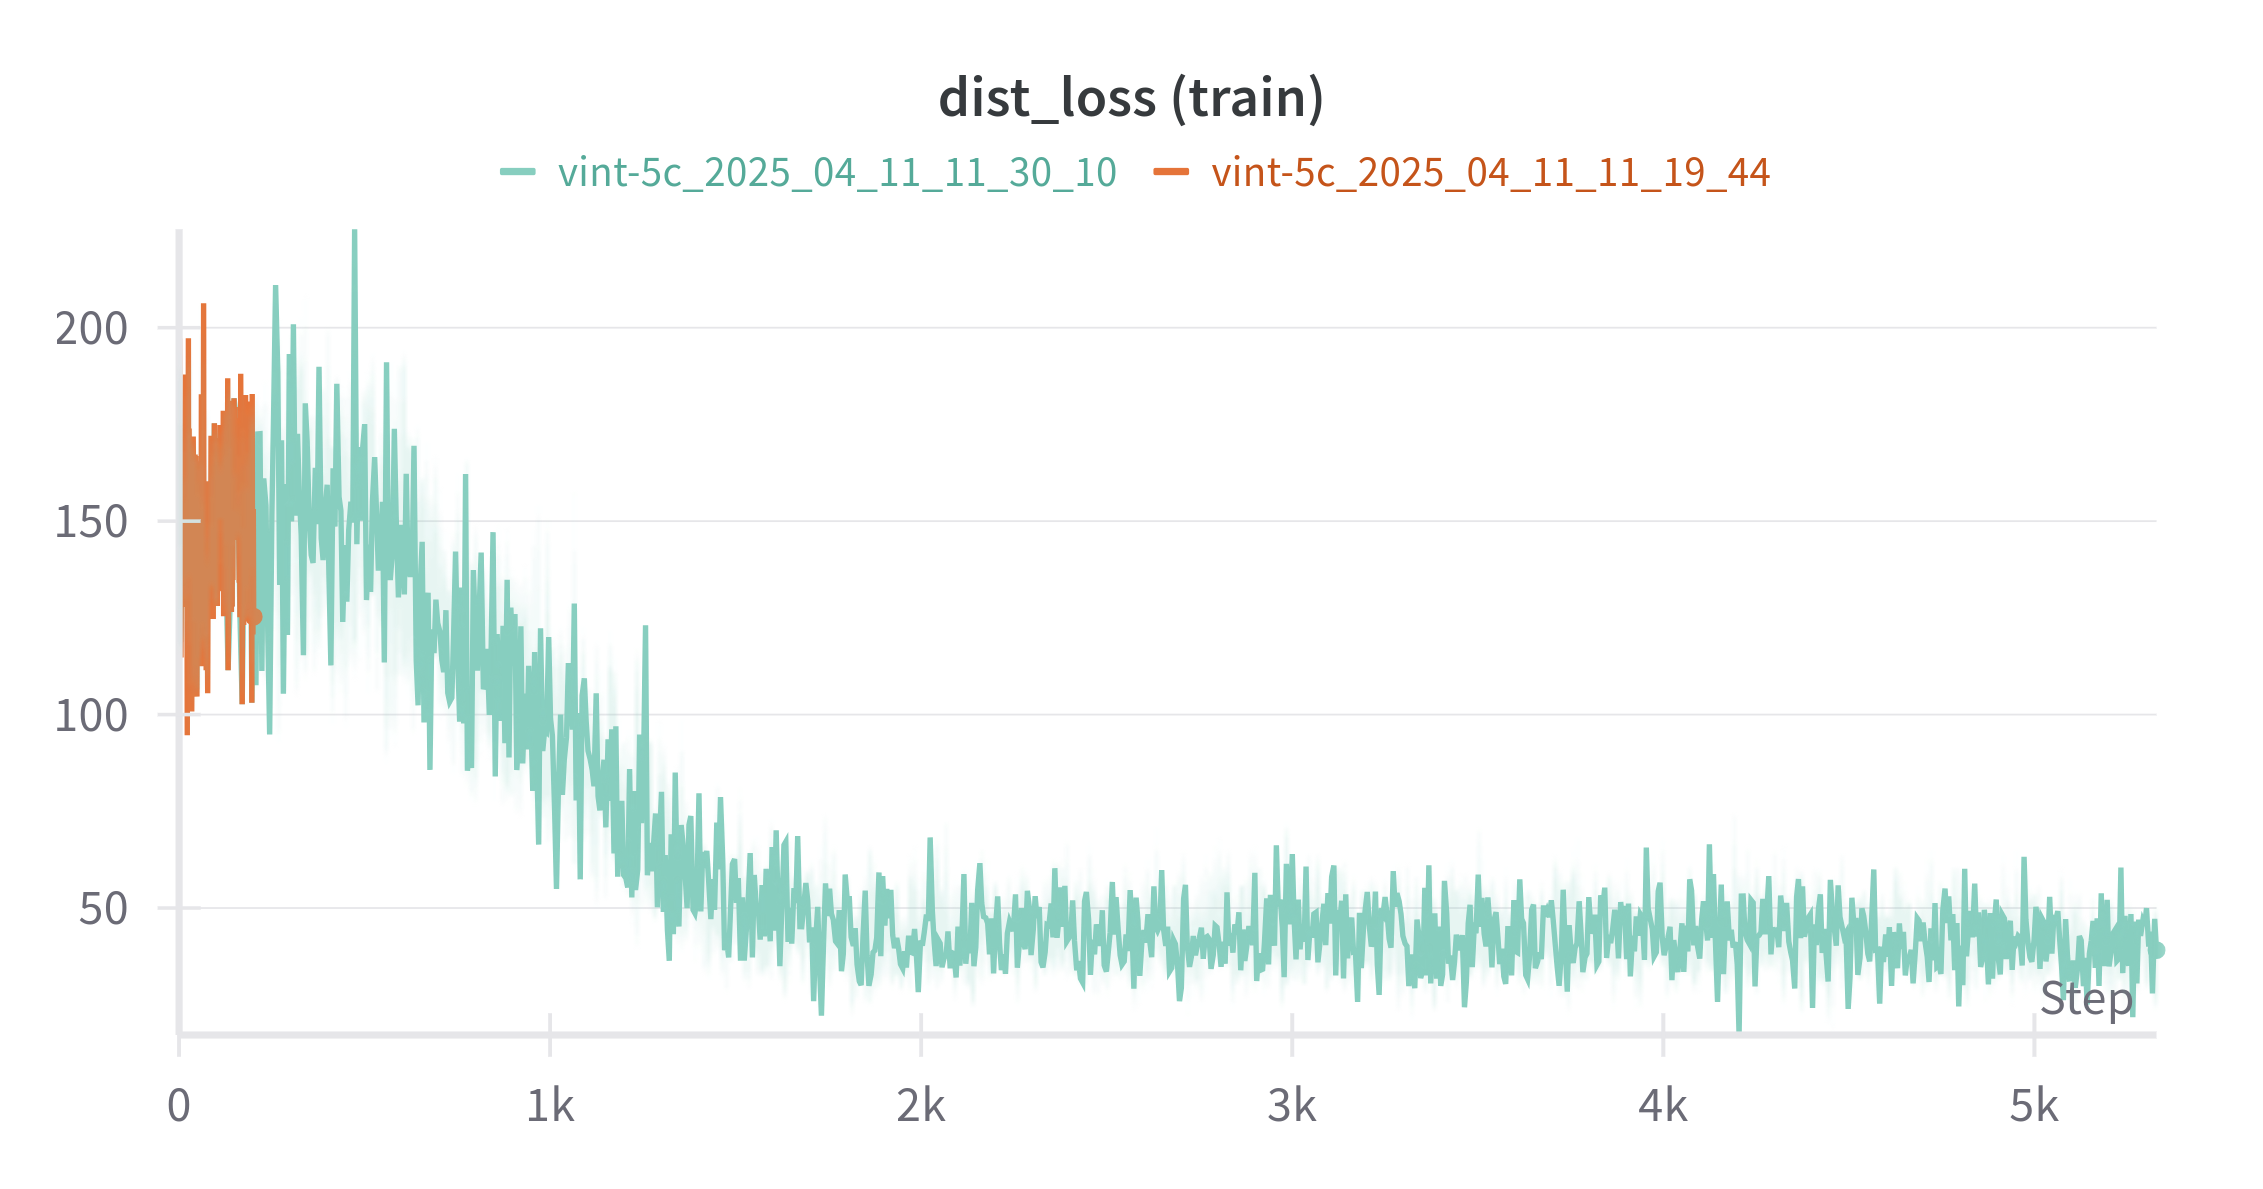
\includegraphics[width=\textwidth]{images/vint_dist_loss.png}
        \caption{Distance Loss on Training Set for ViNT}
        \label{fig:vint_action_loss_train}
    \end{subfigure}
    \hfill
    \begin{subfigure}[b]{0.48\textwidth}
        \centering
        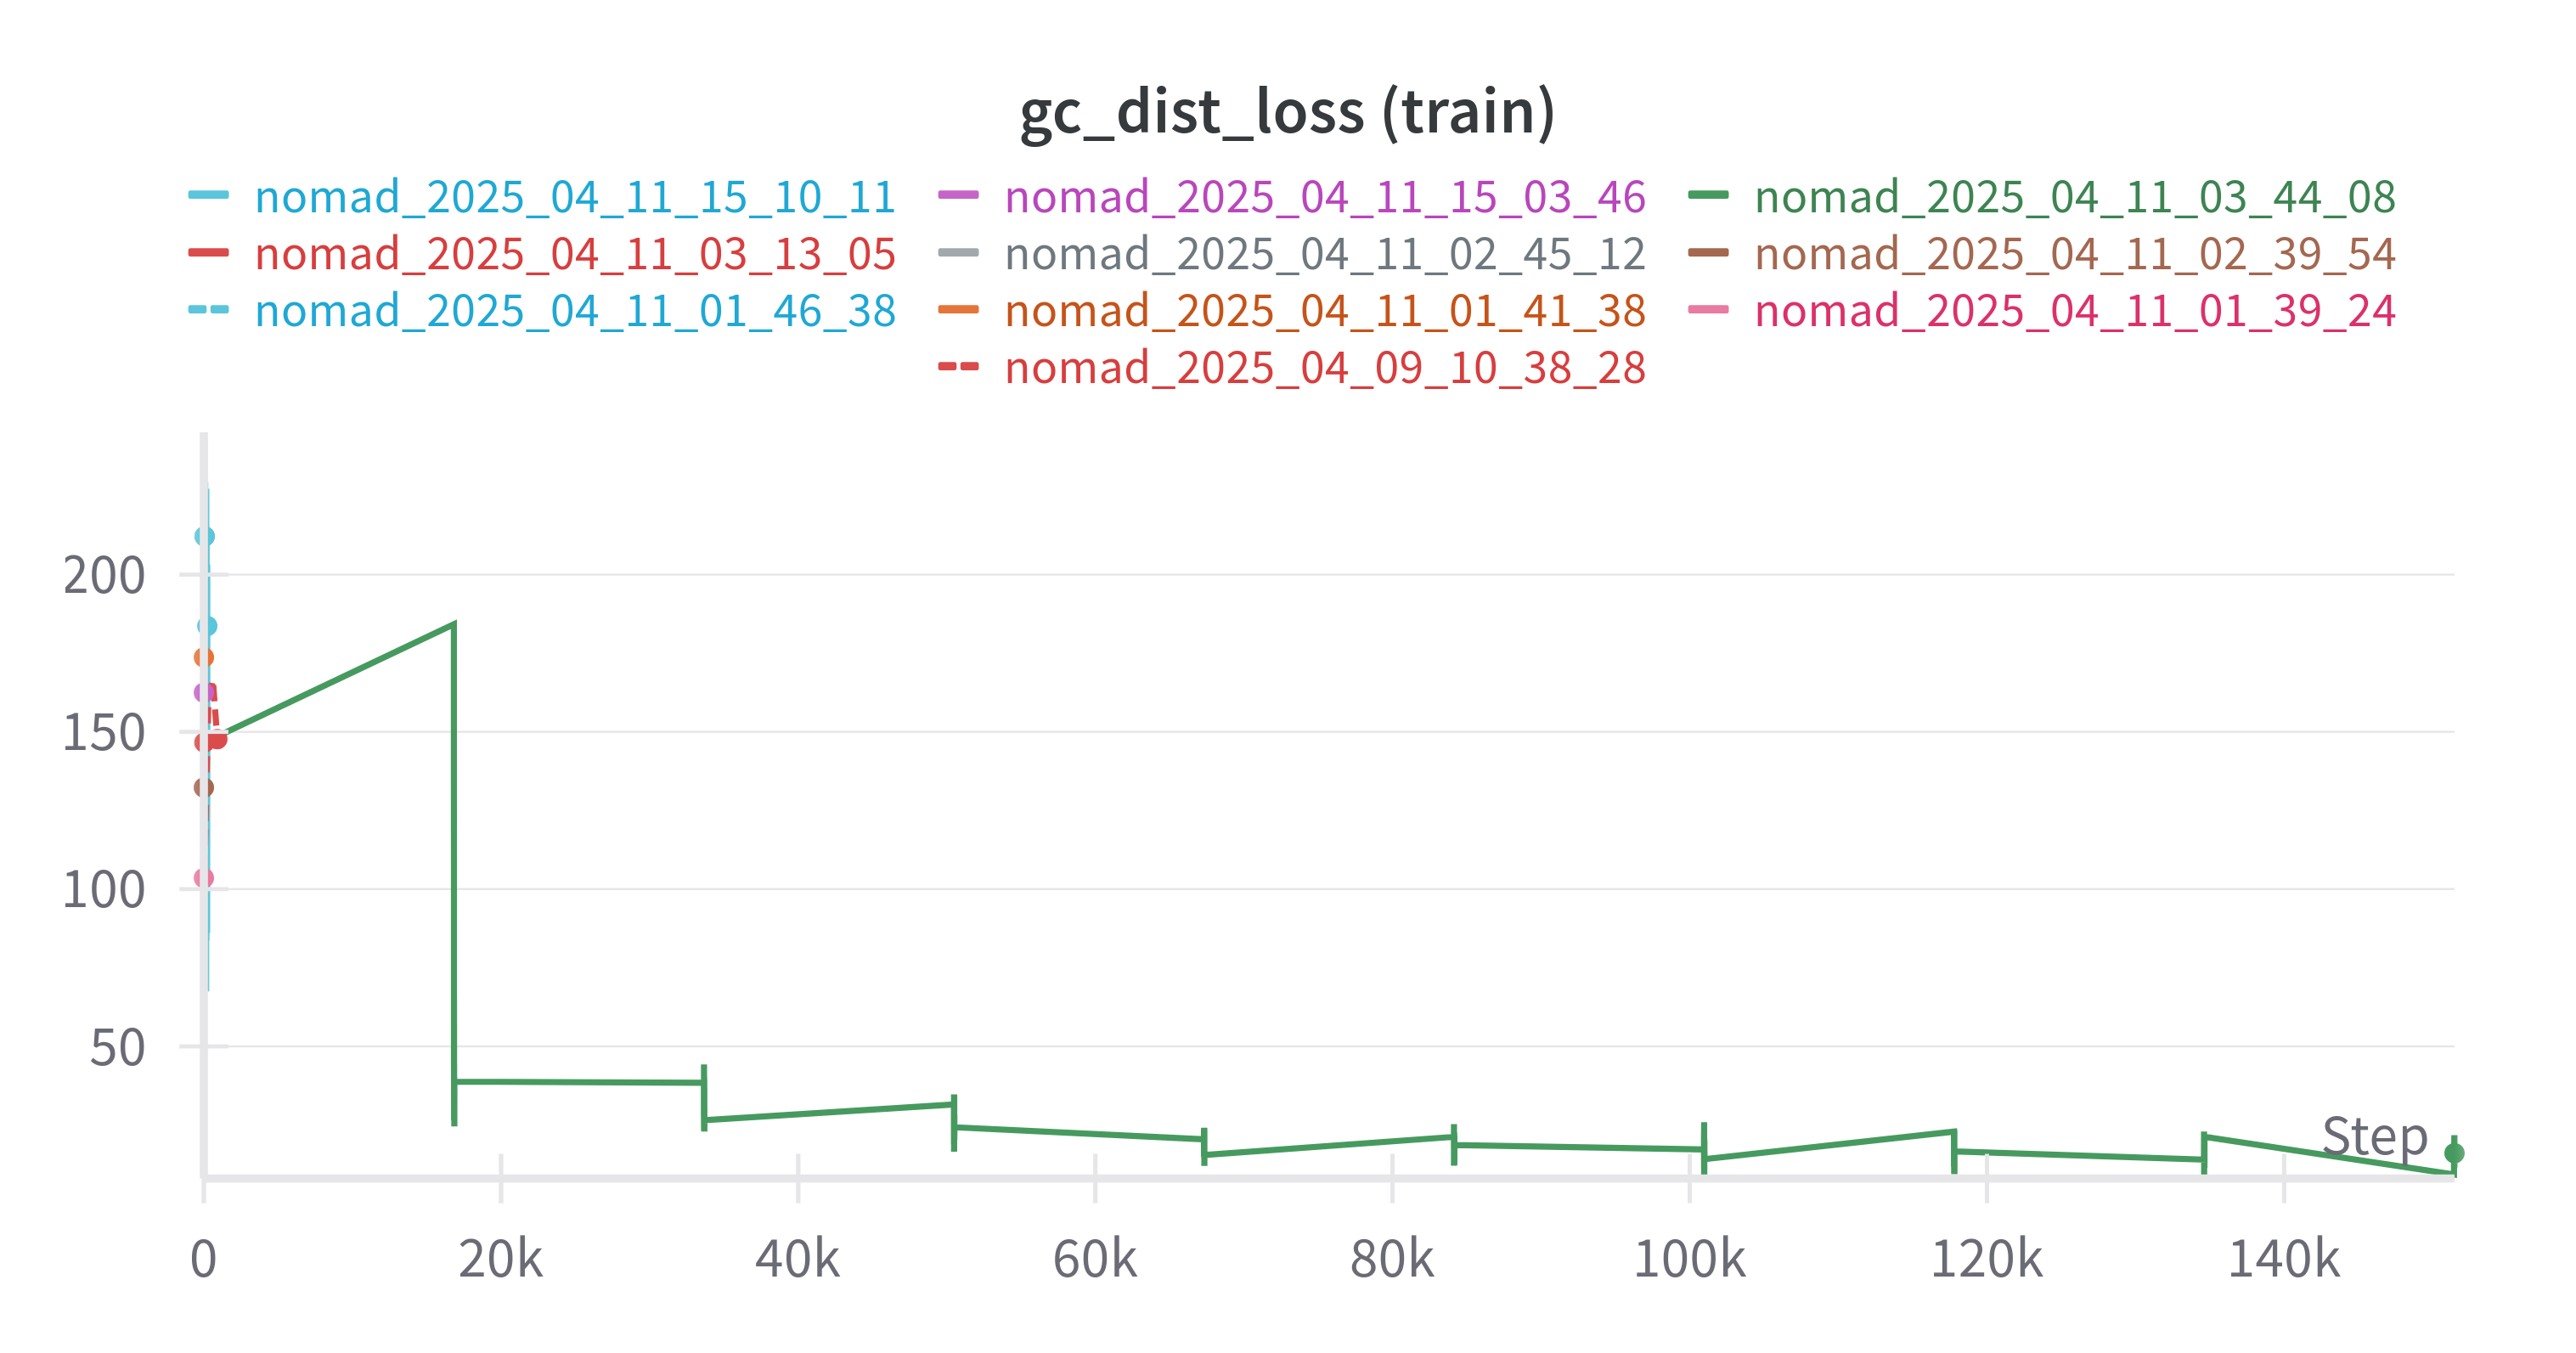
\includegraphics[width=\textwidth]{images/gc_distloss_nomad.png}
        \caption{Distance Loss on Training Set for NoMaD}
        \label{fig:vint_action_loss_val}
    \end{subfigure}
    \begin{subfigure}[b]{0.48\textwidth}
        \centering
        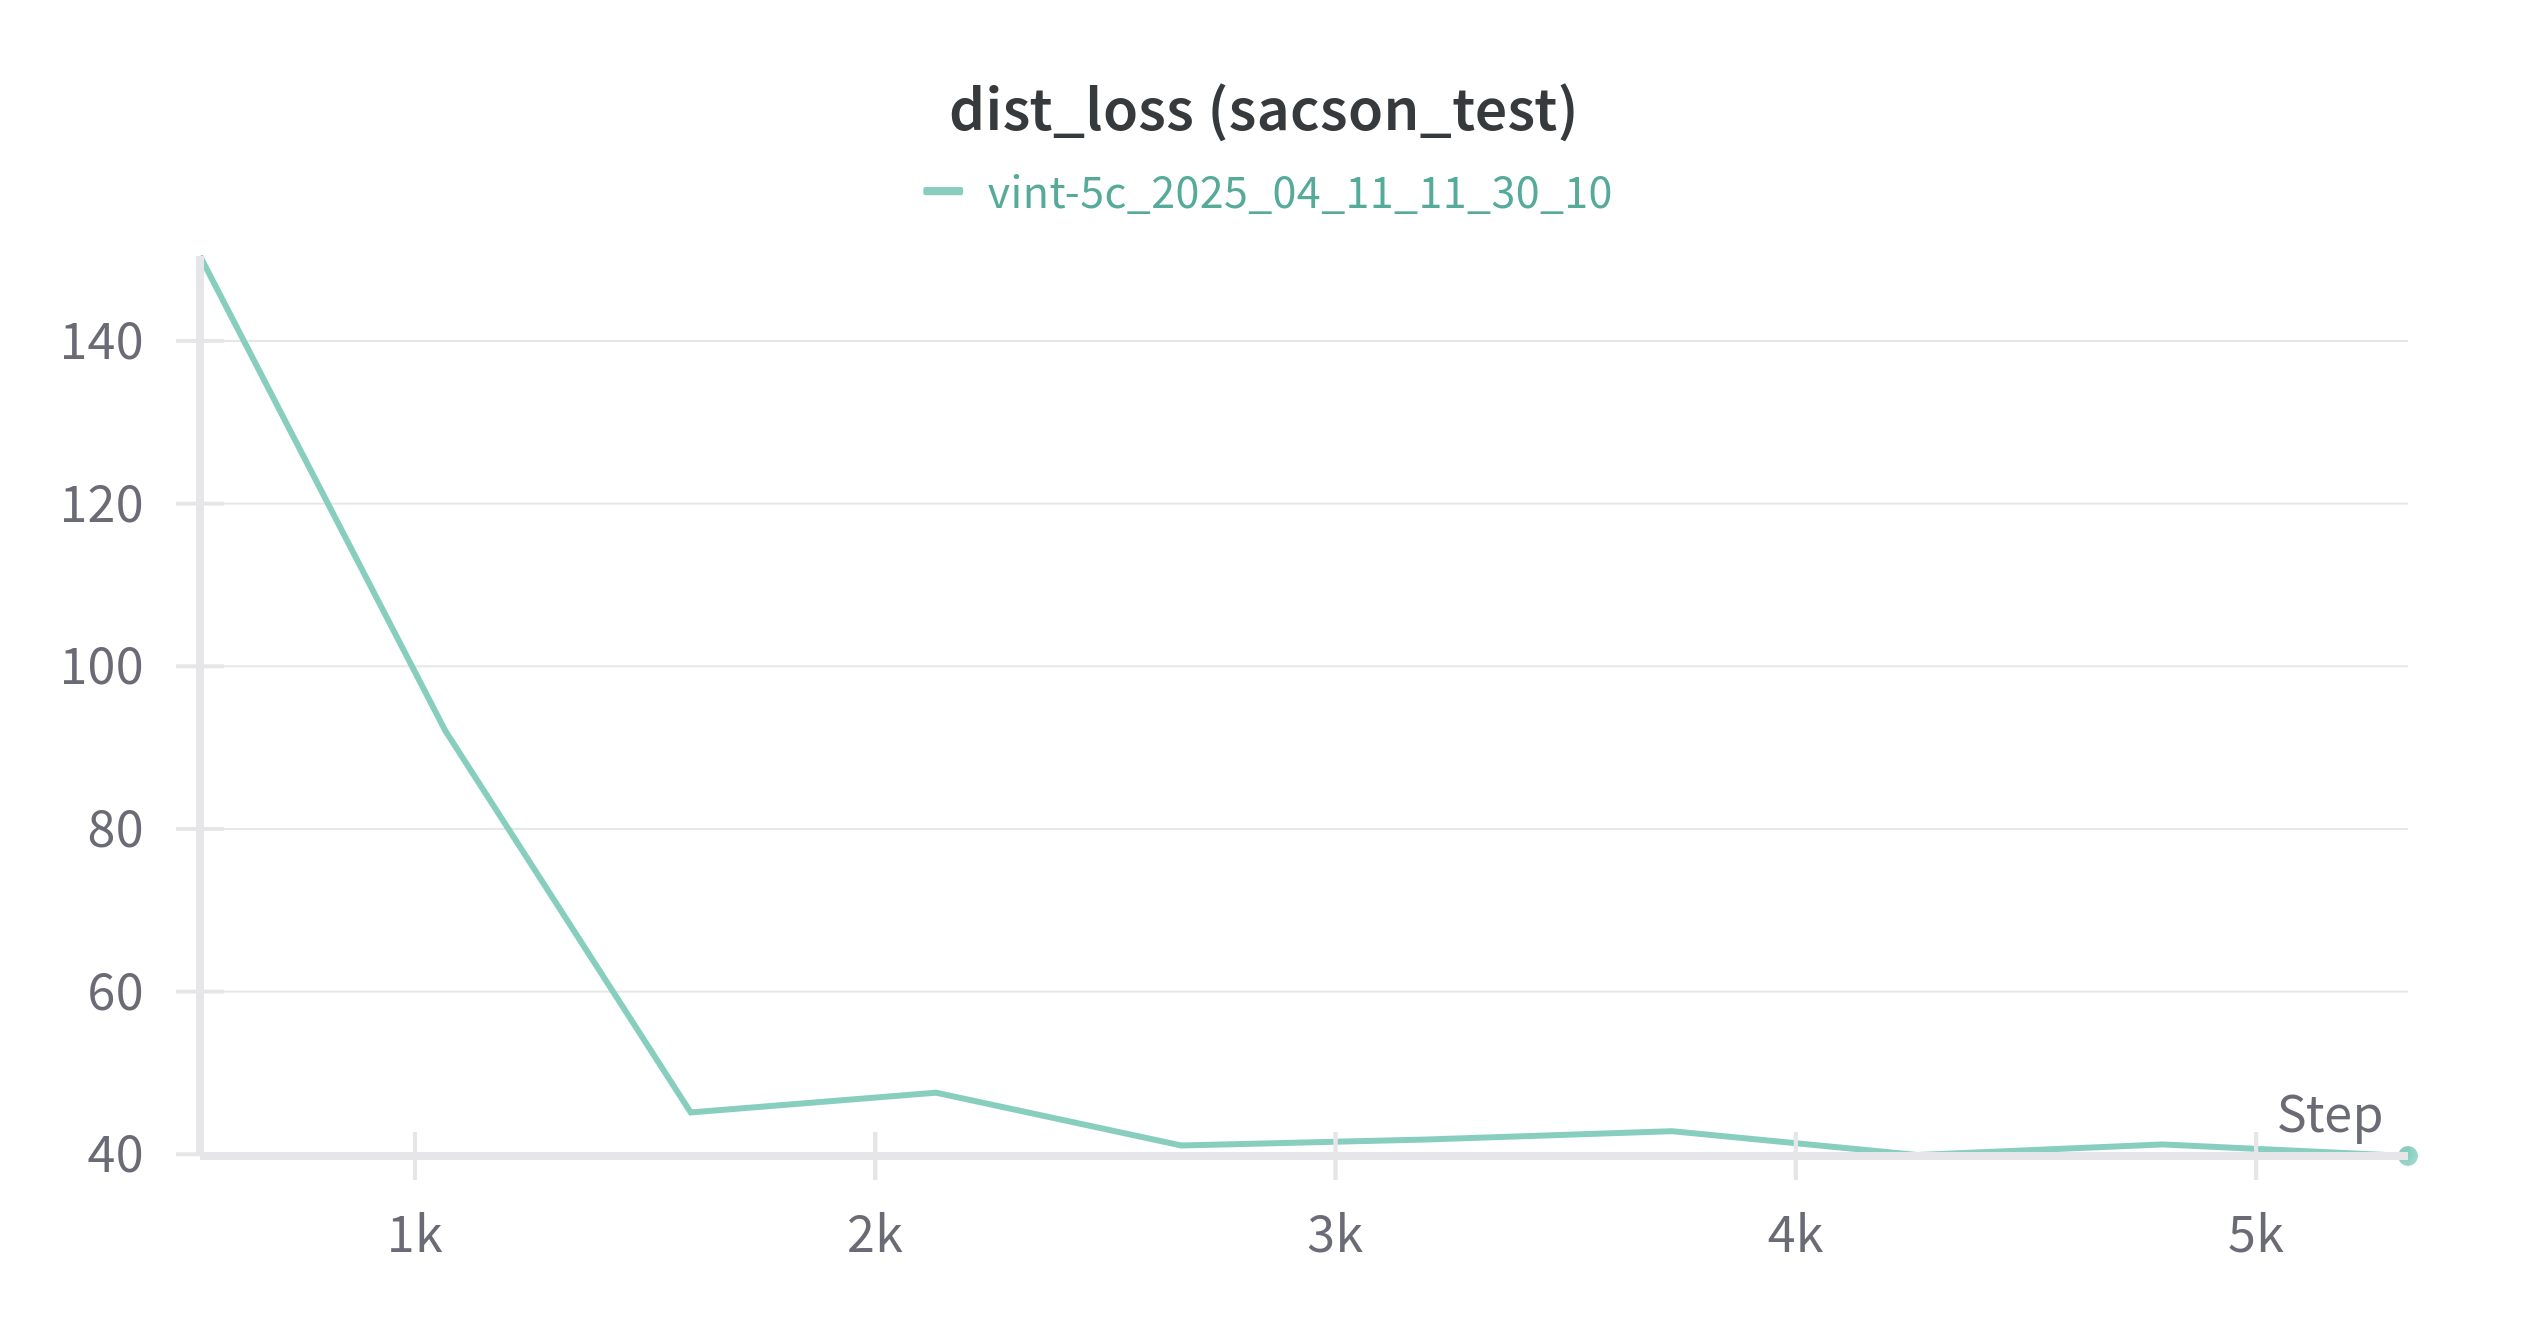
\includegraphics[width=\textwidth]{images/dist_test_vint.png}
        \caption{Distance Loss on Validation Set for ViNT}
        \label{fig:gc_dist_loss_val}
    \end{subfigure}
    \hfill
    \begin{subfigure}[b]{0.48\textwidth}
        \centering
        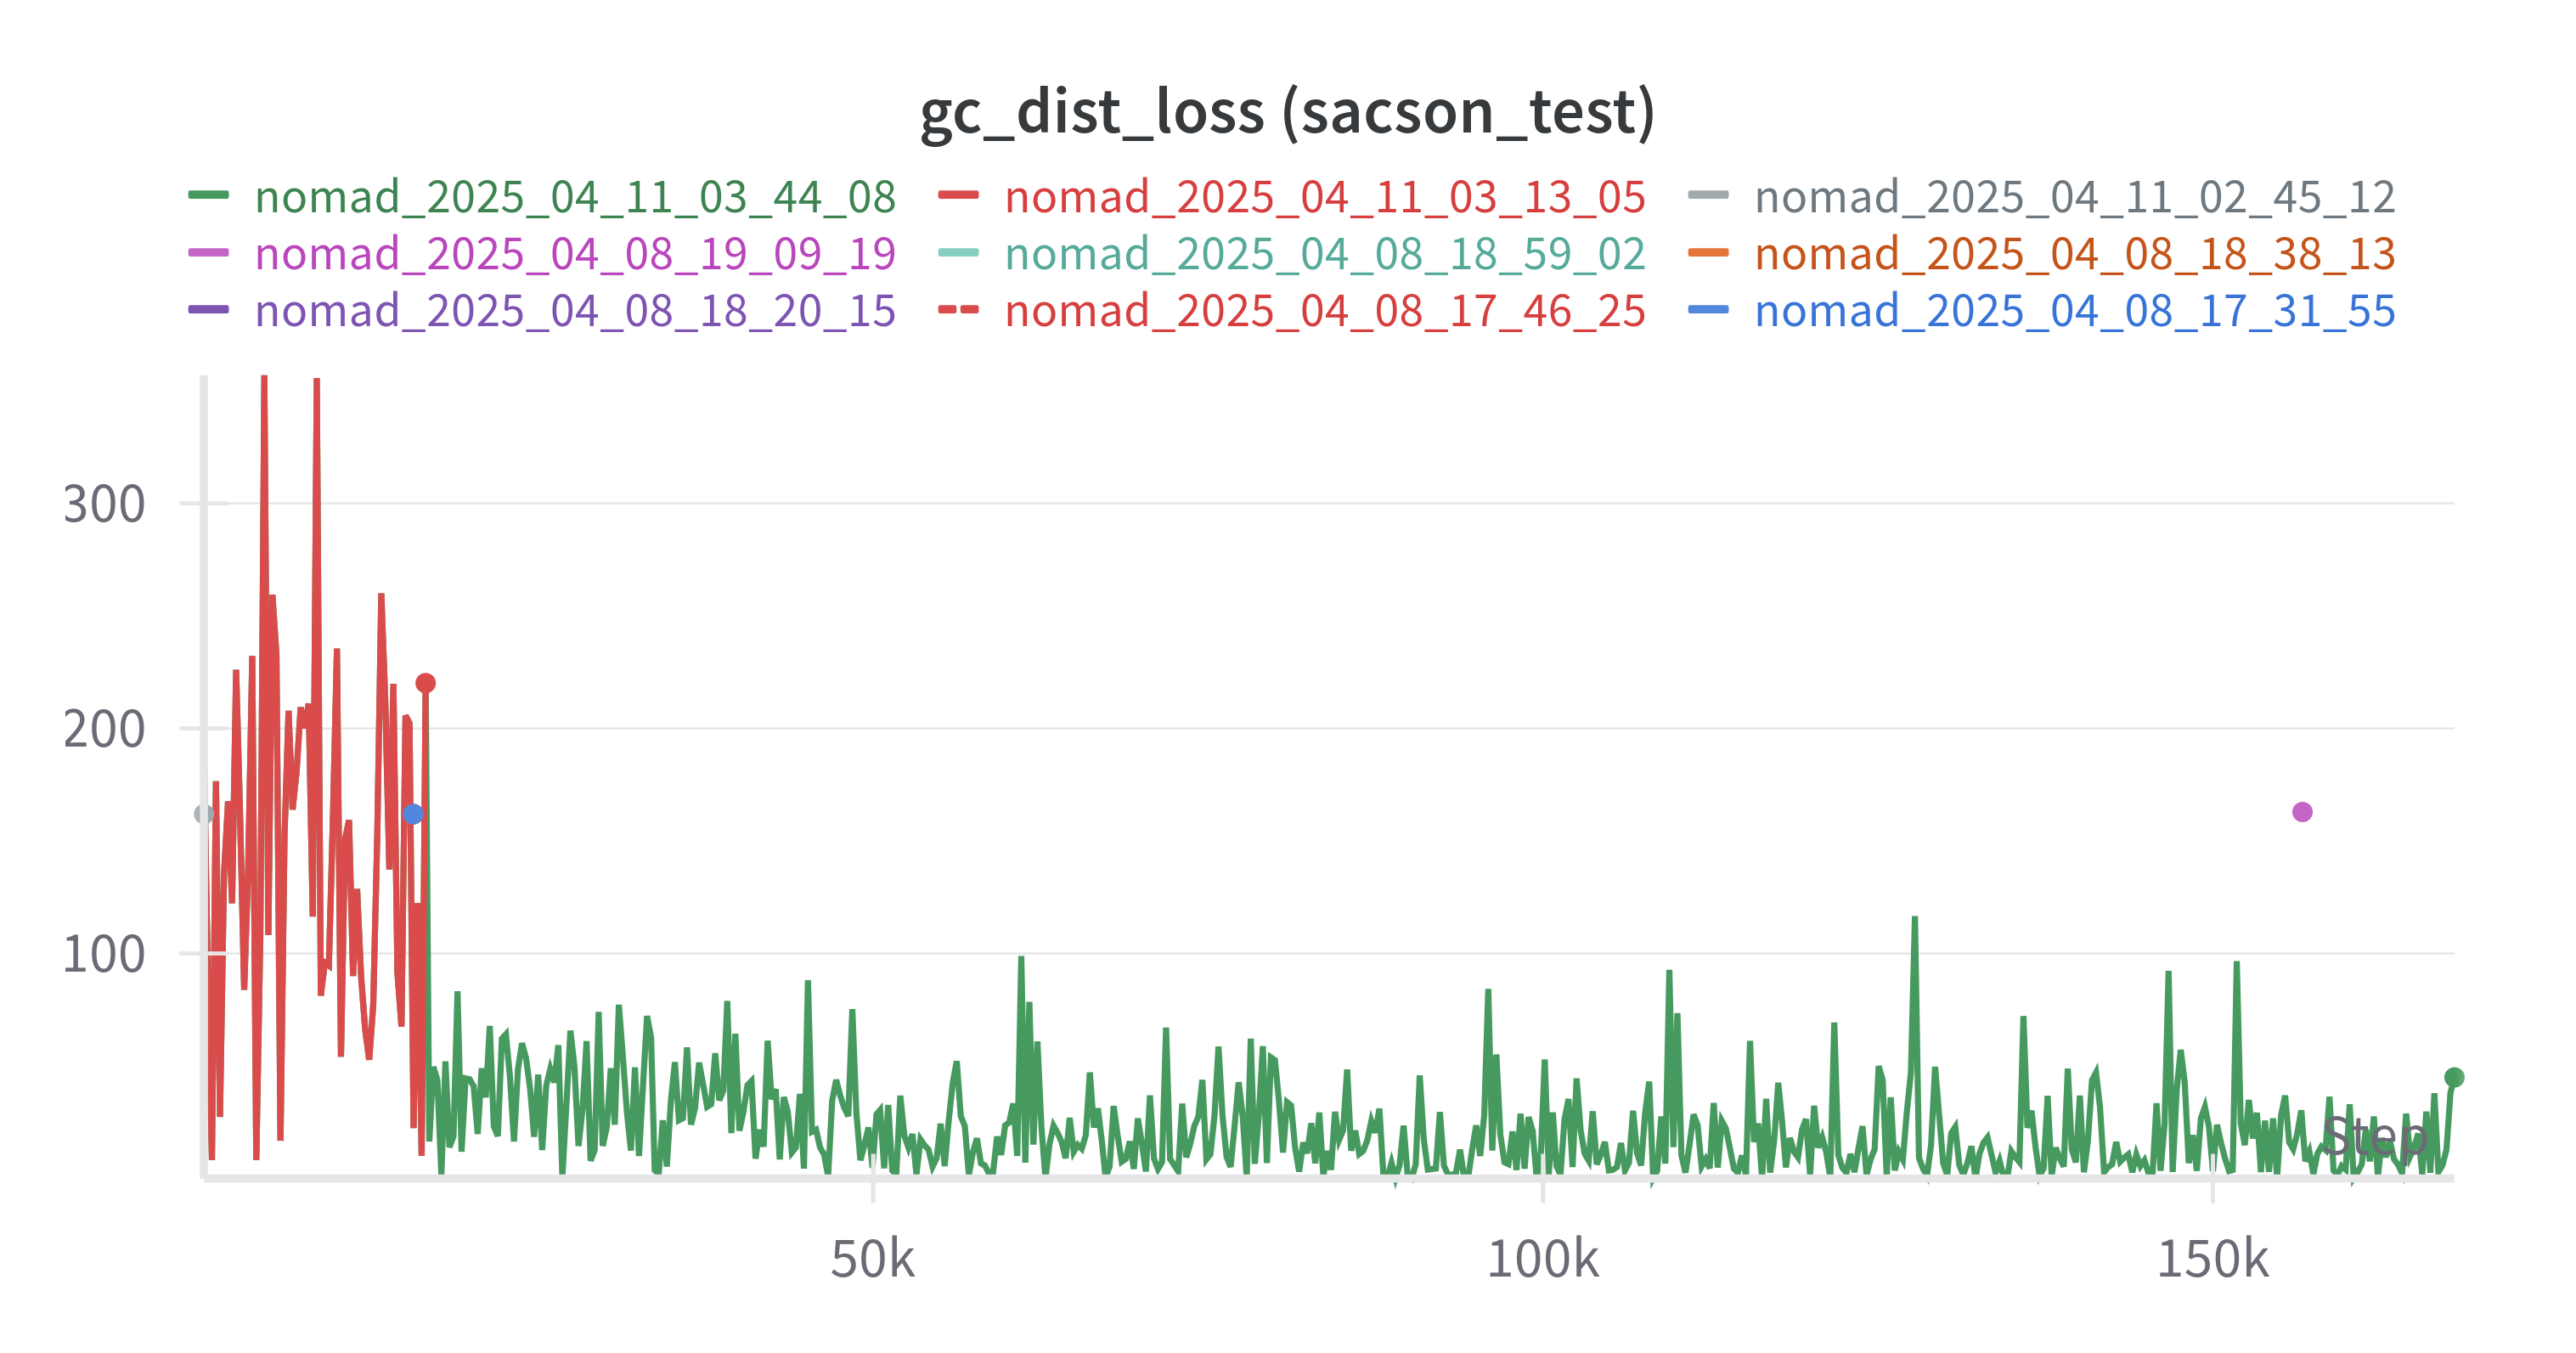
\includegraphics[width=\textwidth]{images/gc_dist_loss_test.png}
        \caption{Distance Loss on Validation Set for ViNT}
        \label{fig:gc_dist_loss_val_vint}
    \end{subfigure}
    \caption{Distance loss comparison between ViNT and NoMaD on training and validation sets.}
\end{figure}
\begin{figure}[H]
    \centering
    \begin{subfigure}[b]{0.48\textwidth}
        \centering
        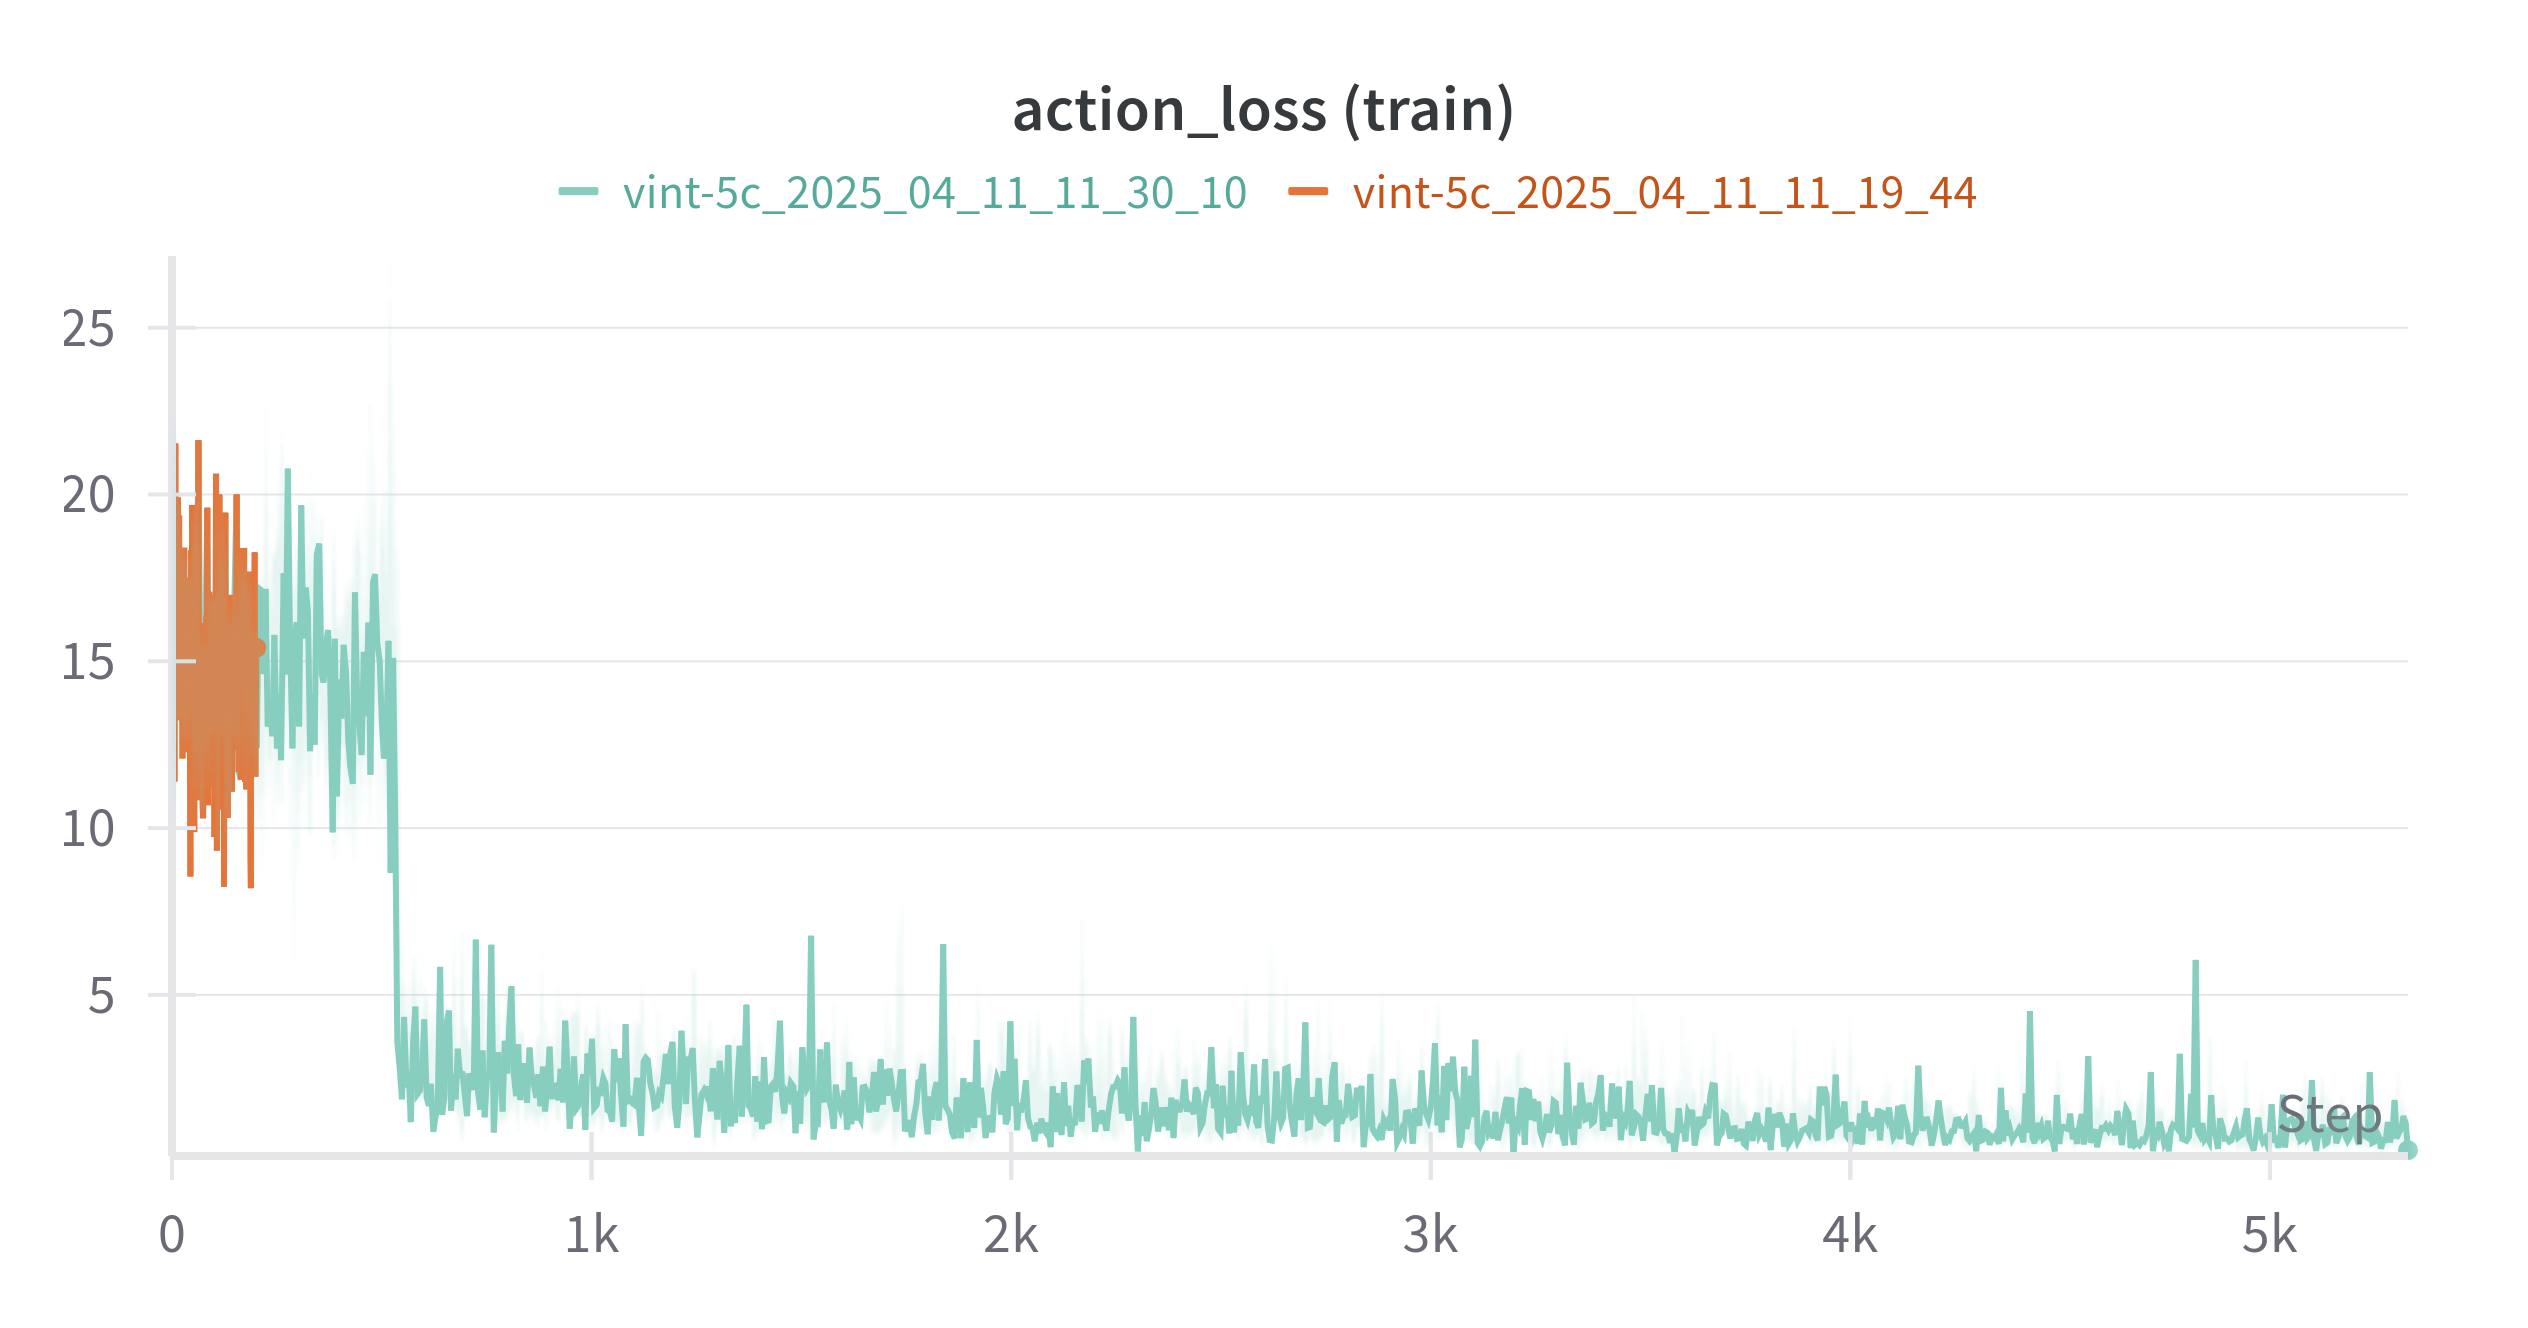
\includegraphics[width=\textwidth]{images/action_train_vint.png}
        \caption{Action Loss on Training Set for ViNT}
        \label{fig:vint_action_loss_train}
    \end{subfigure}
    \hfill
    \begin{subfigure}[b]{0.48\textwidth}
        \centering
        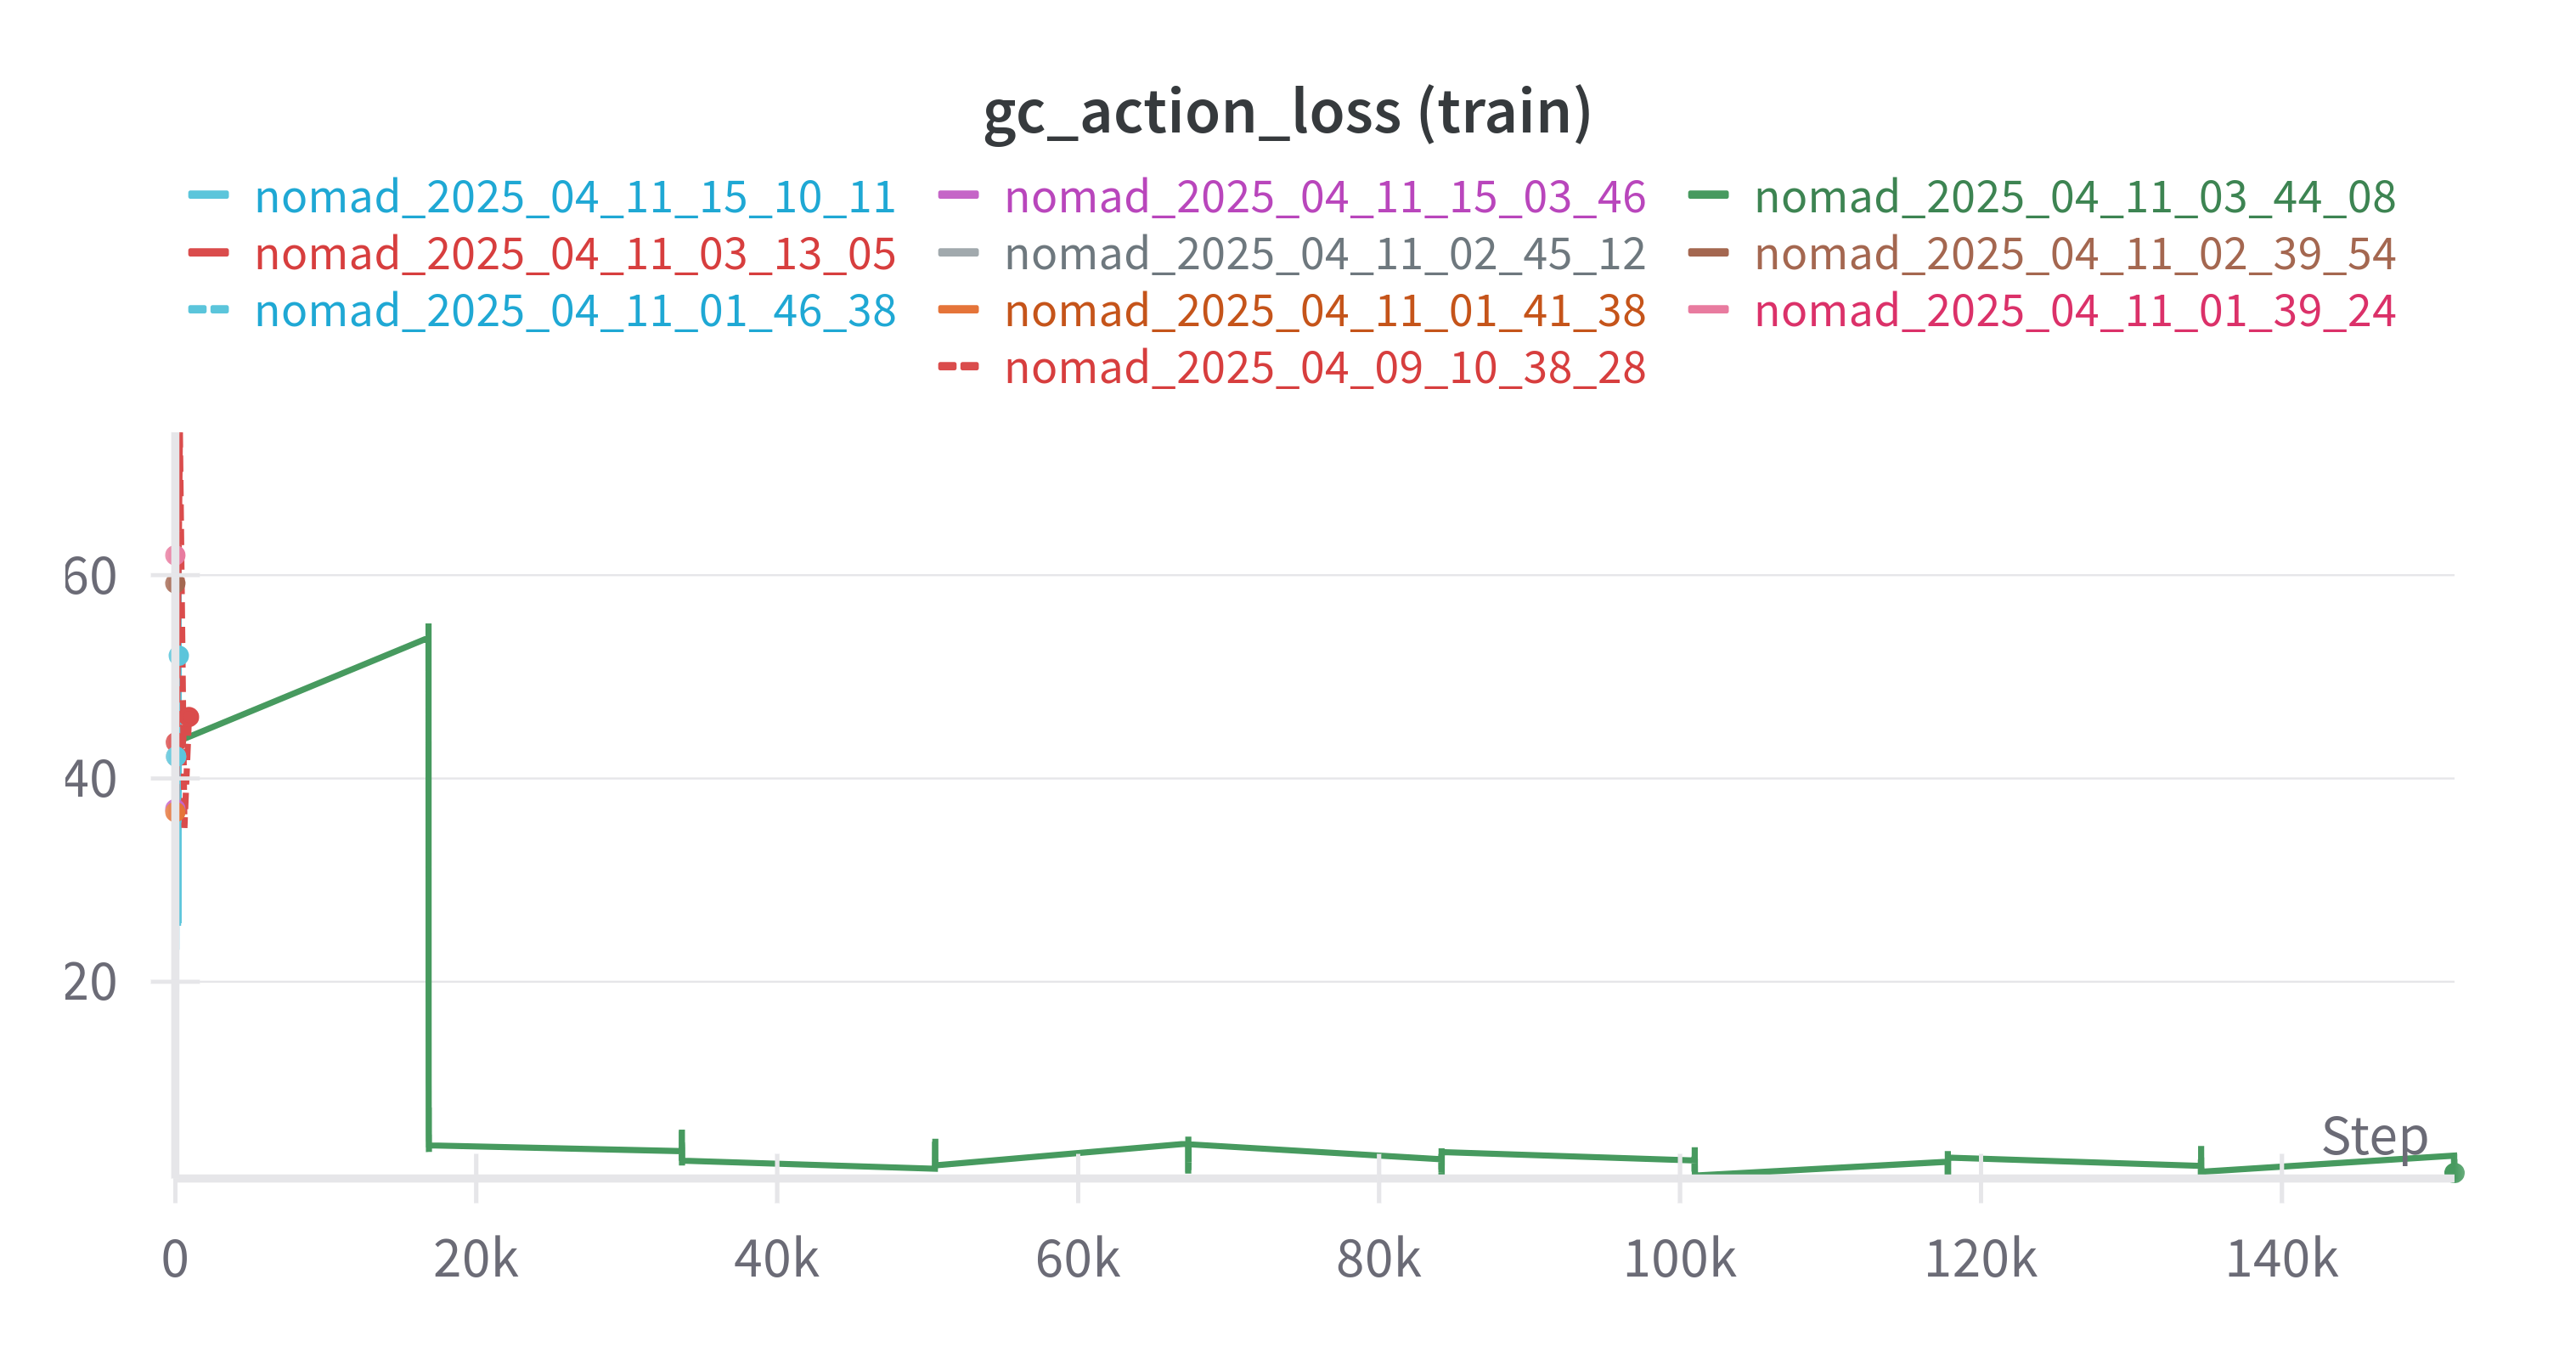
\includegraphics[width=\textwidth]{images/gc_actionloss_nomad.png}
        \caption{Action Loss on Training Set for NoMaD}
        \label{fig:vint_action_loss_val}
    \end{subfigure}
    \begin{subfigure}[b]{0.48\textwidth}
        \centering
        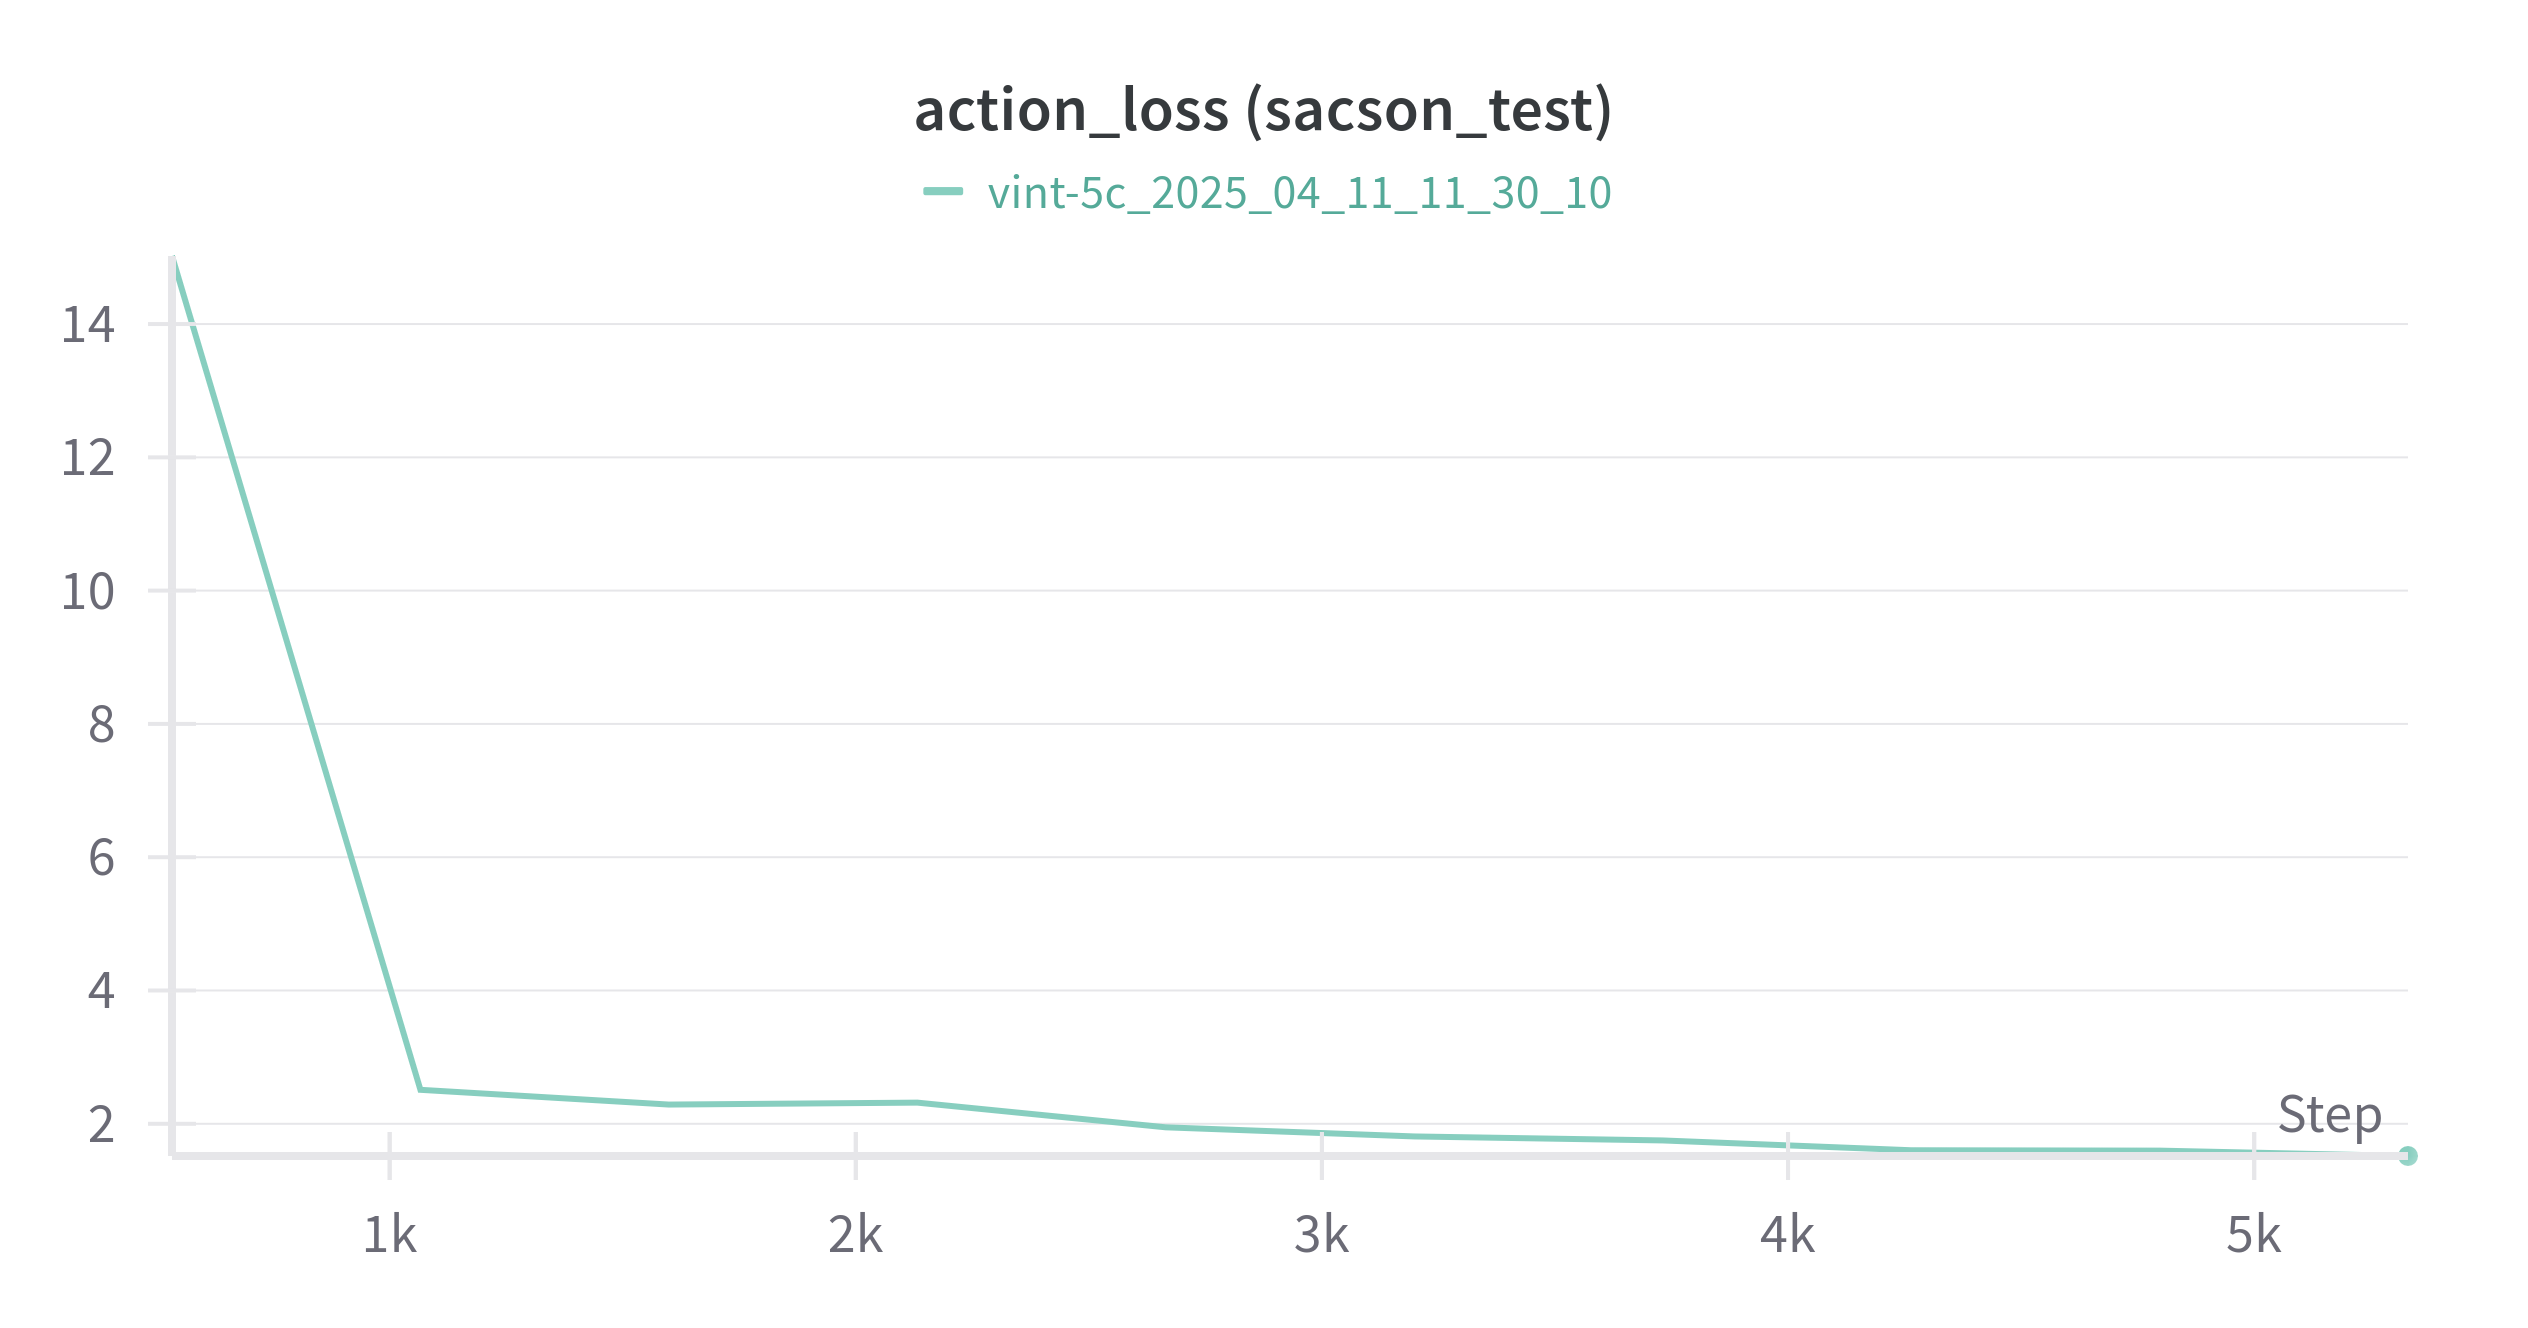
\includegraphics[width=\textwidth]{images/action_test_vint.png}
        \caption{Action Loss on Validation Set for ViNT}
        \label{fig:gc_action_loss_val_vint}
    \end{subfigure}
    \hfill
    \begin{subfigure}[b]{0.48\textwidth}
        \centering
        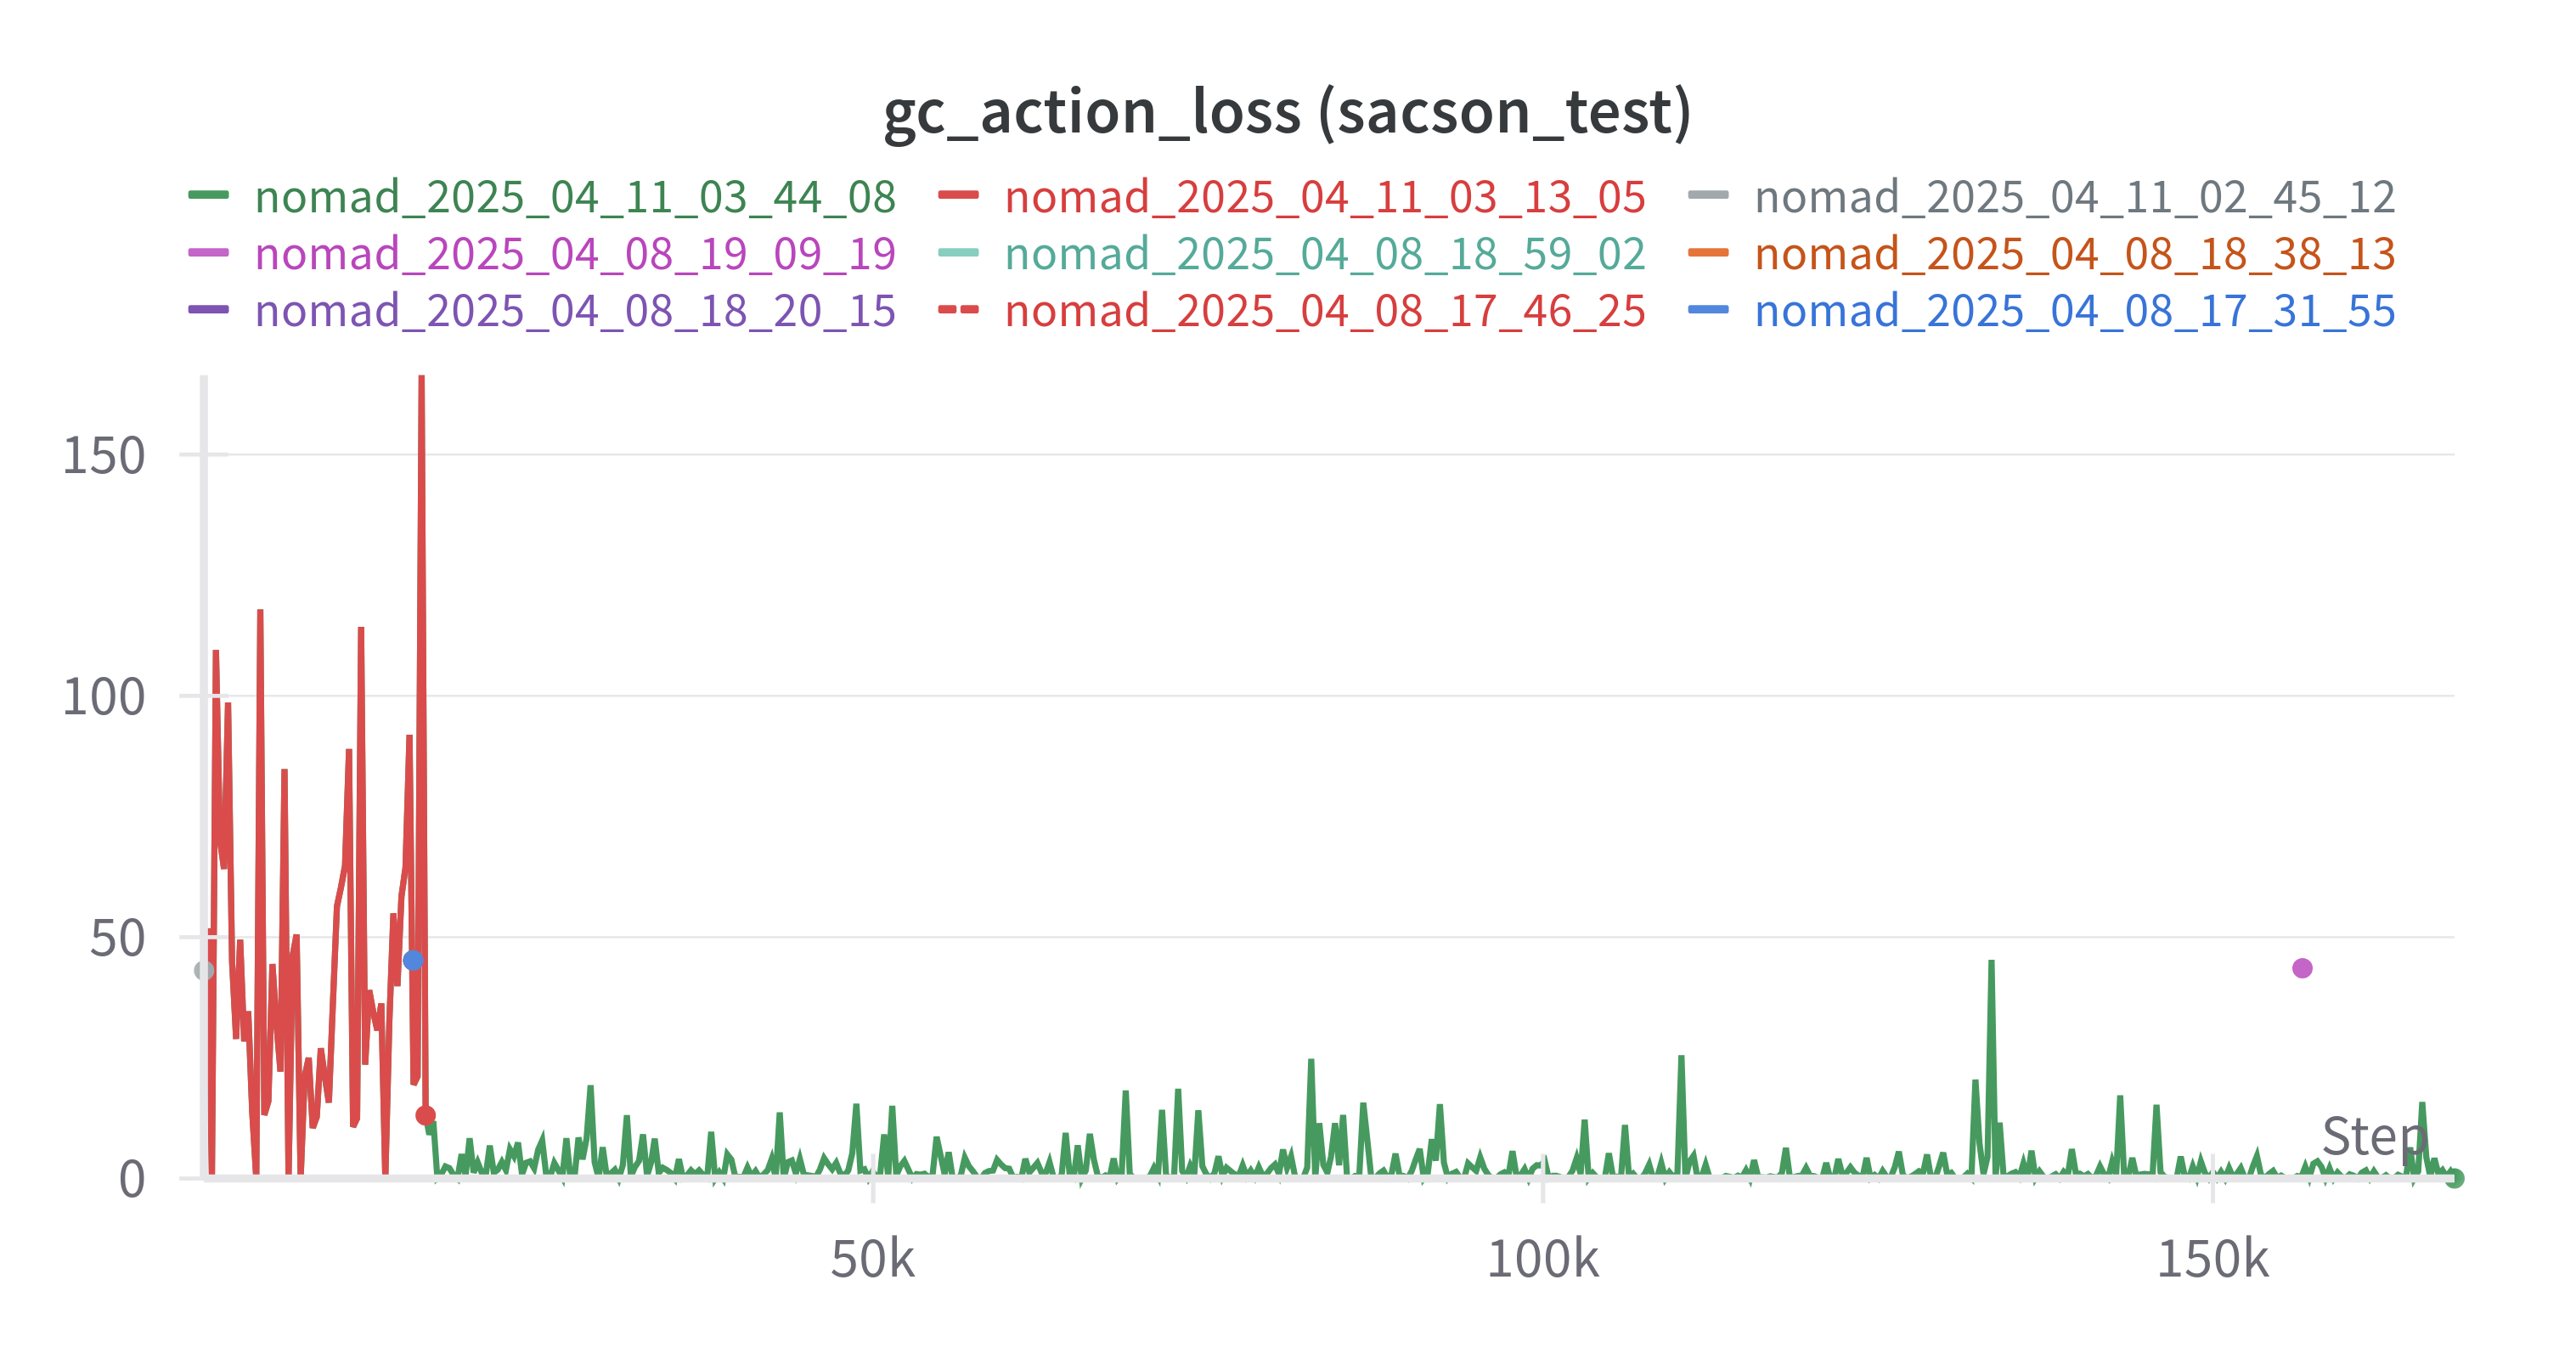
\includegraphics[width=\textwidth]{images/gc_actionloss_test_nomad.png}
        \caption{Action Loss on Validation Set for NoMaD}
        \label{fig:gc_action_loss_val_vint}
    \end{subfigure}
    \caption{Action loss comparison between ViNT and NoMaD on training and validation sets.}
\end{figure}

Here are some plots from WandB comparing the two models(NoMaD and ViNT)\\
\subsection*{Action Cosine Similarity}
\begin{figure}[H]
    \centering
    \begin{subfigure}[b]{0.48\textwidth}
        \centering
        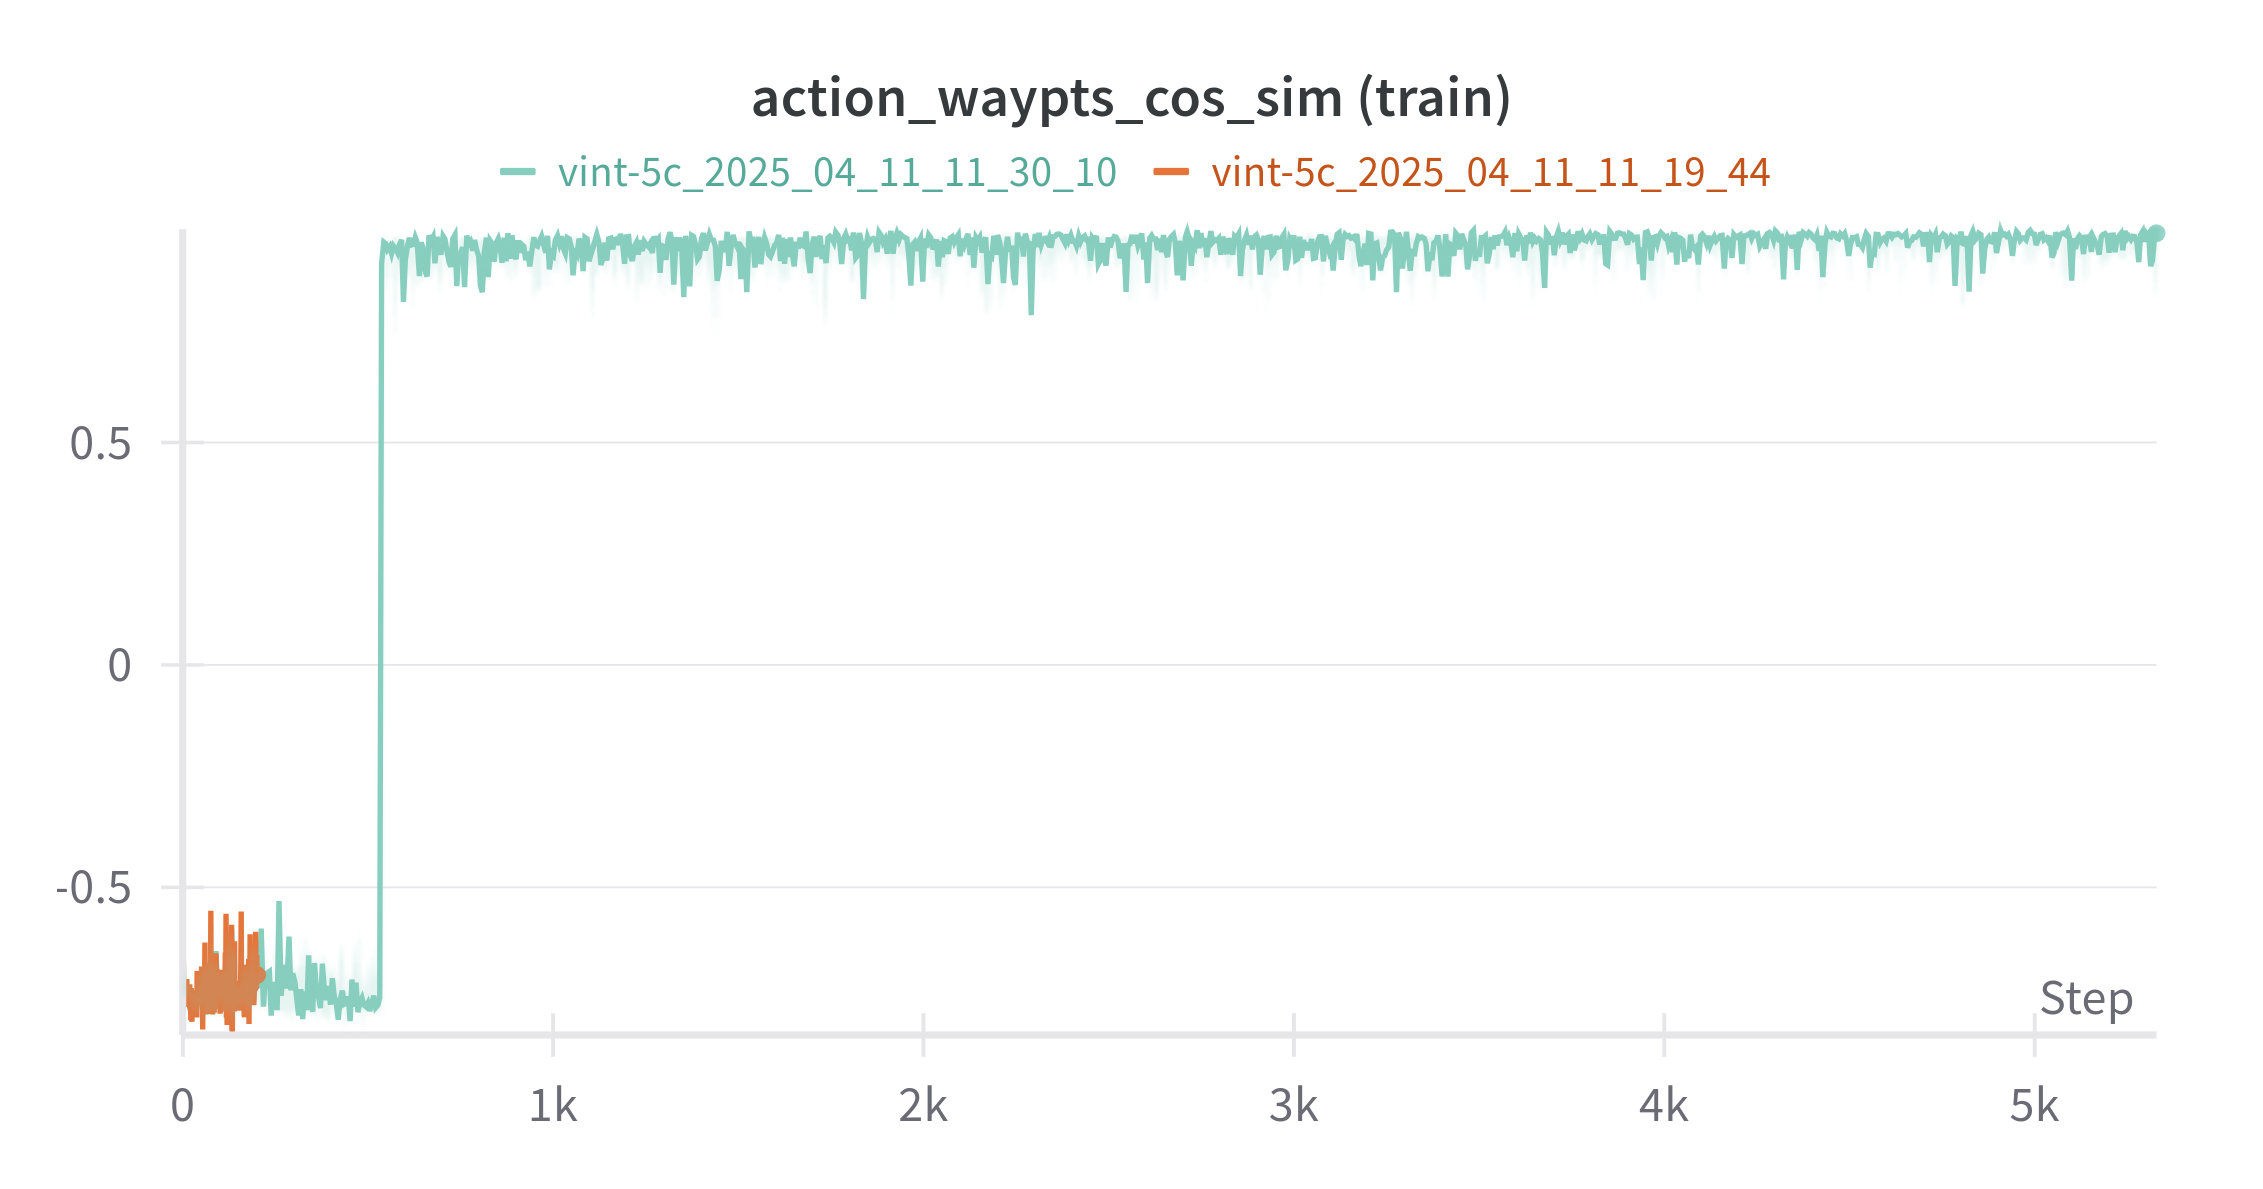
\includegraphics[width=\textwidth]{images/action_sim_train_vint.png}
        \label{fig:action_train_vint}
        \caption{ViNT Action Cosine Similarity on Training Set}
    \end{subfigure}
    \hfill
    \begin{subfigure}[b]{0.48\textwidth}
        \centering
        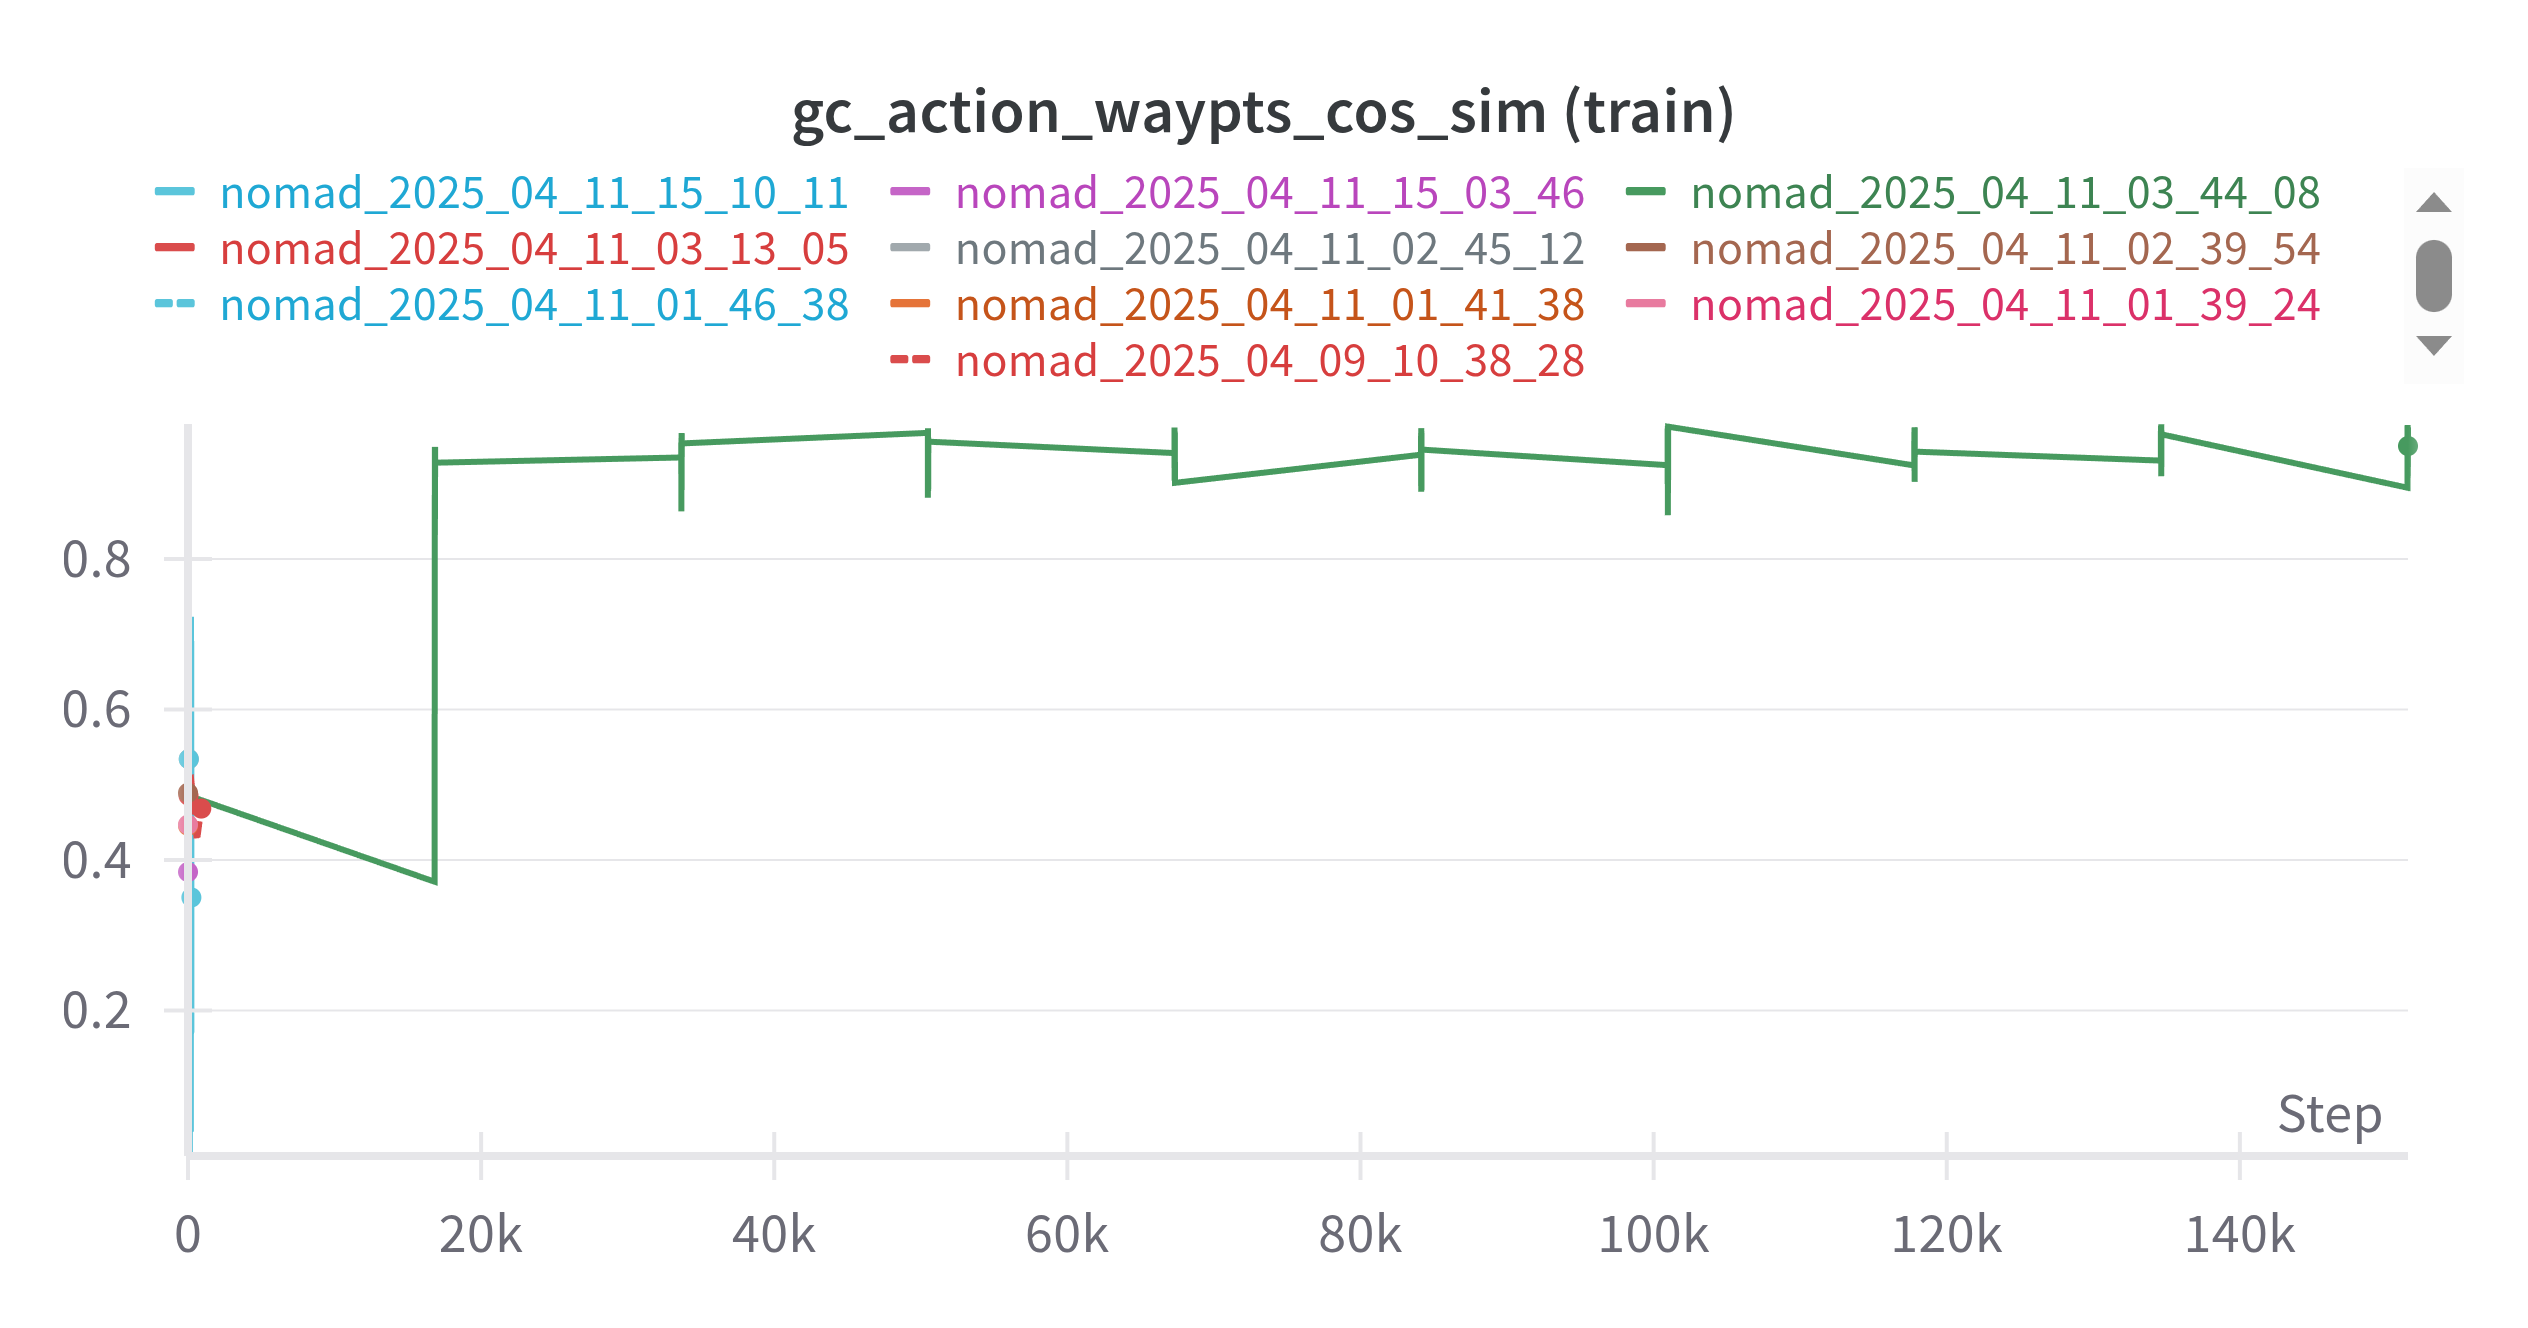
\includegraphics[width=\textwidth]{images/gc_action_waypts_cos_sim_train.png}
        \label{fig:action_train_nomad}
        \caption{NoMaD Action Cosine Similarity on Training Set}
    \end{subfigure}
\end{figure}
\begin{figure}[H]
    \centering
    \begin{subfigure}[b]{0.48\textwidth}
        \centering
        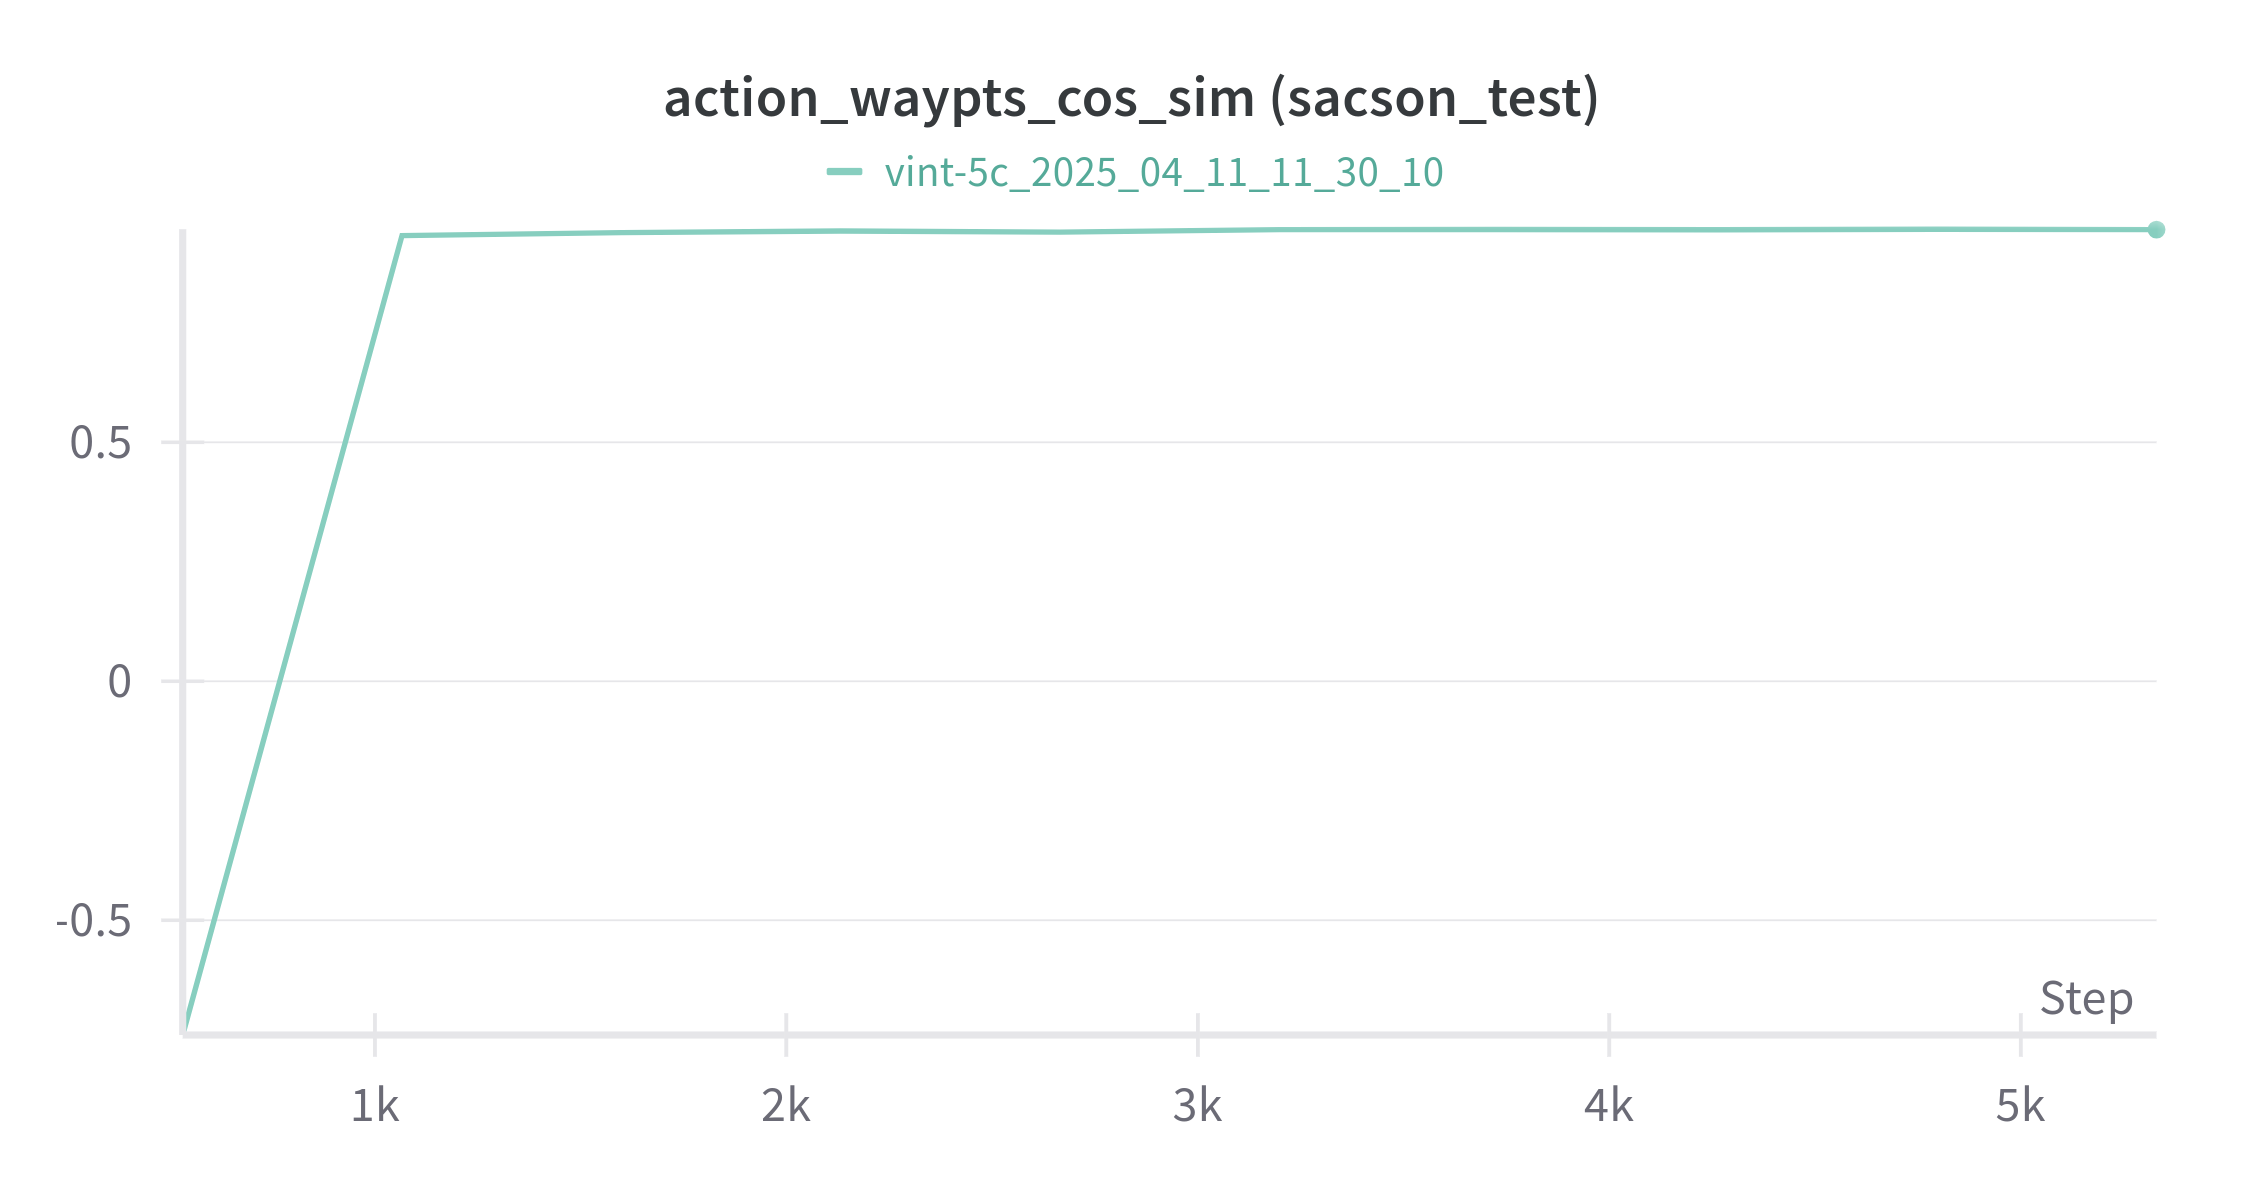
\includegraphics[width=\textwidth]{images/action_sim_test_vint.png}
        \label{fig:action_test_vint}
        \caption{ViNT Action Cosine Similarity on Validation Set}
    \end{subfigure}
    \hfill
    \begin{subfigure}[b]{0.48\textwidth}
        \centering
        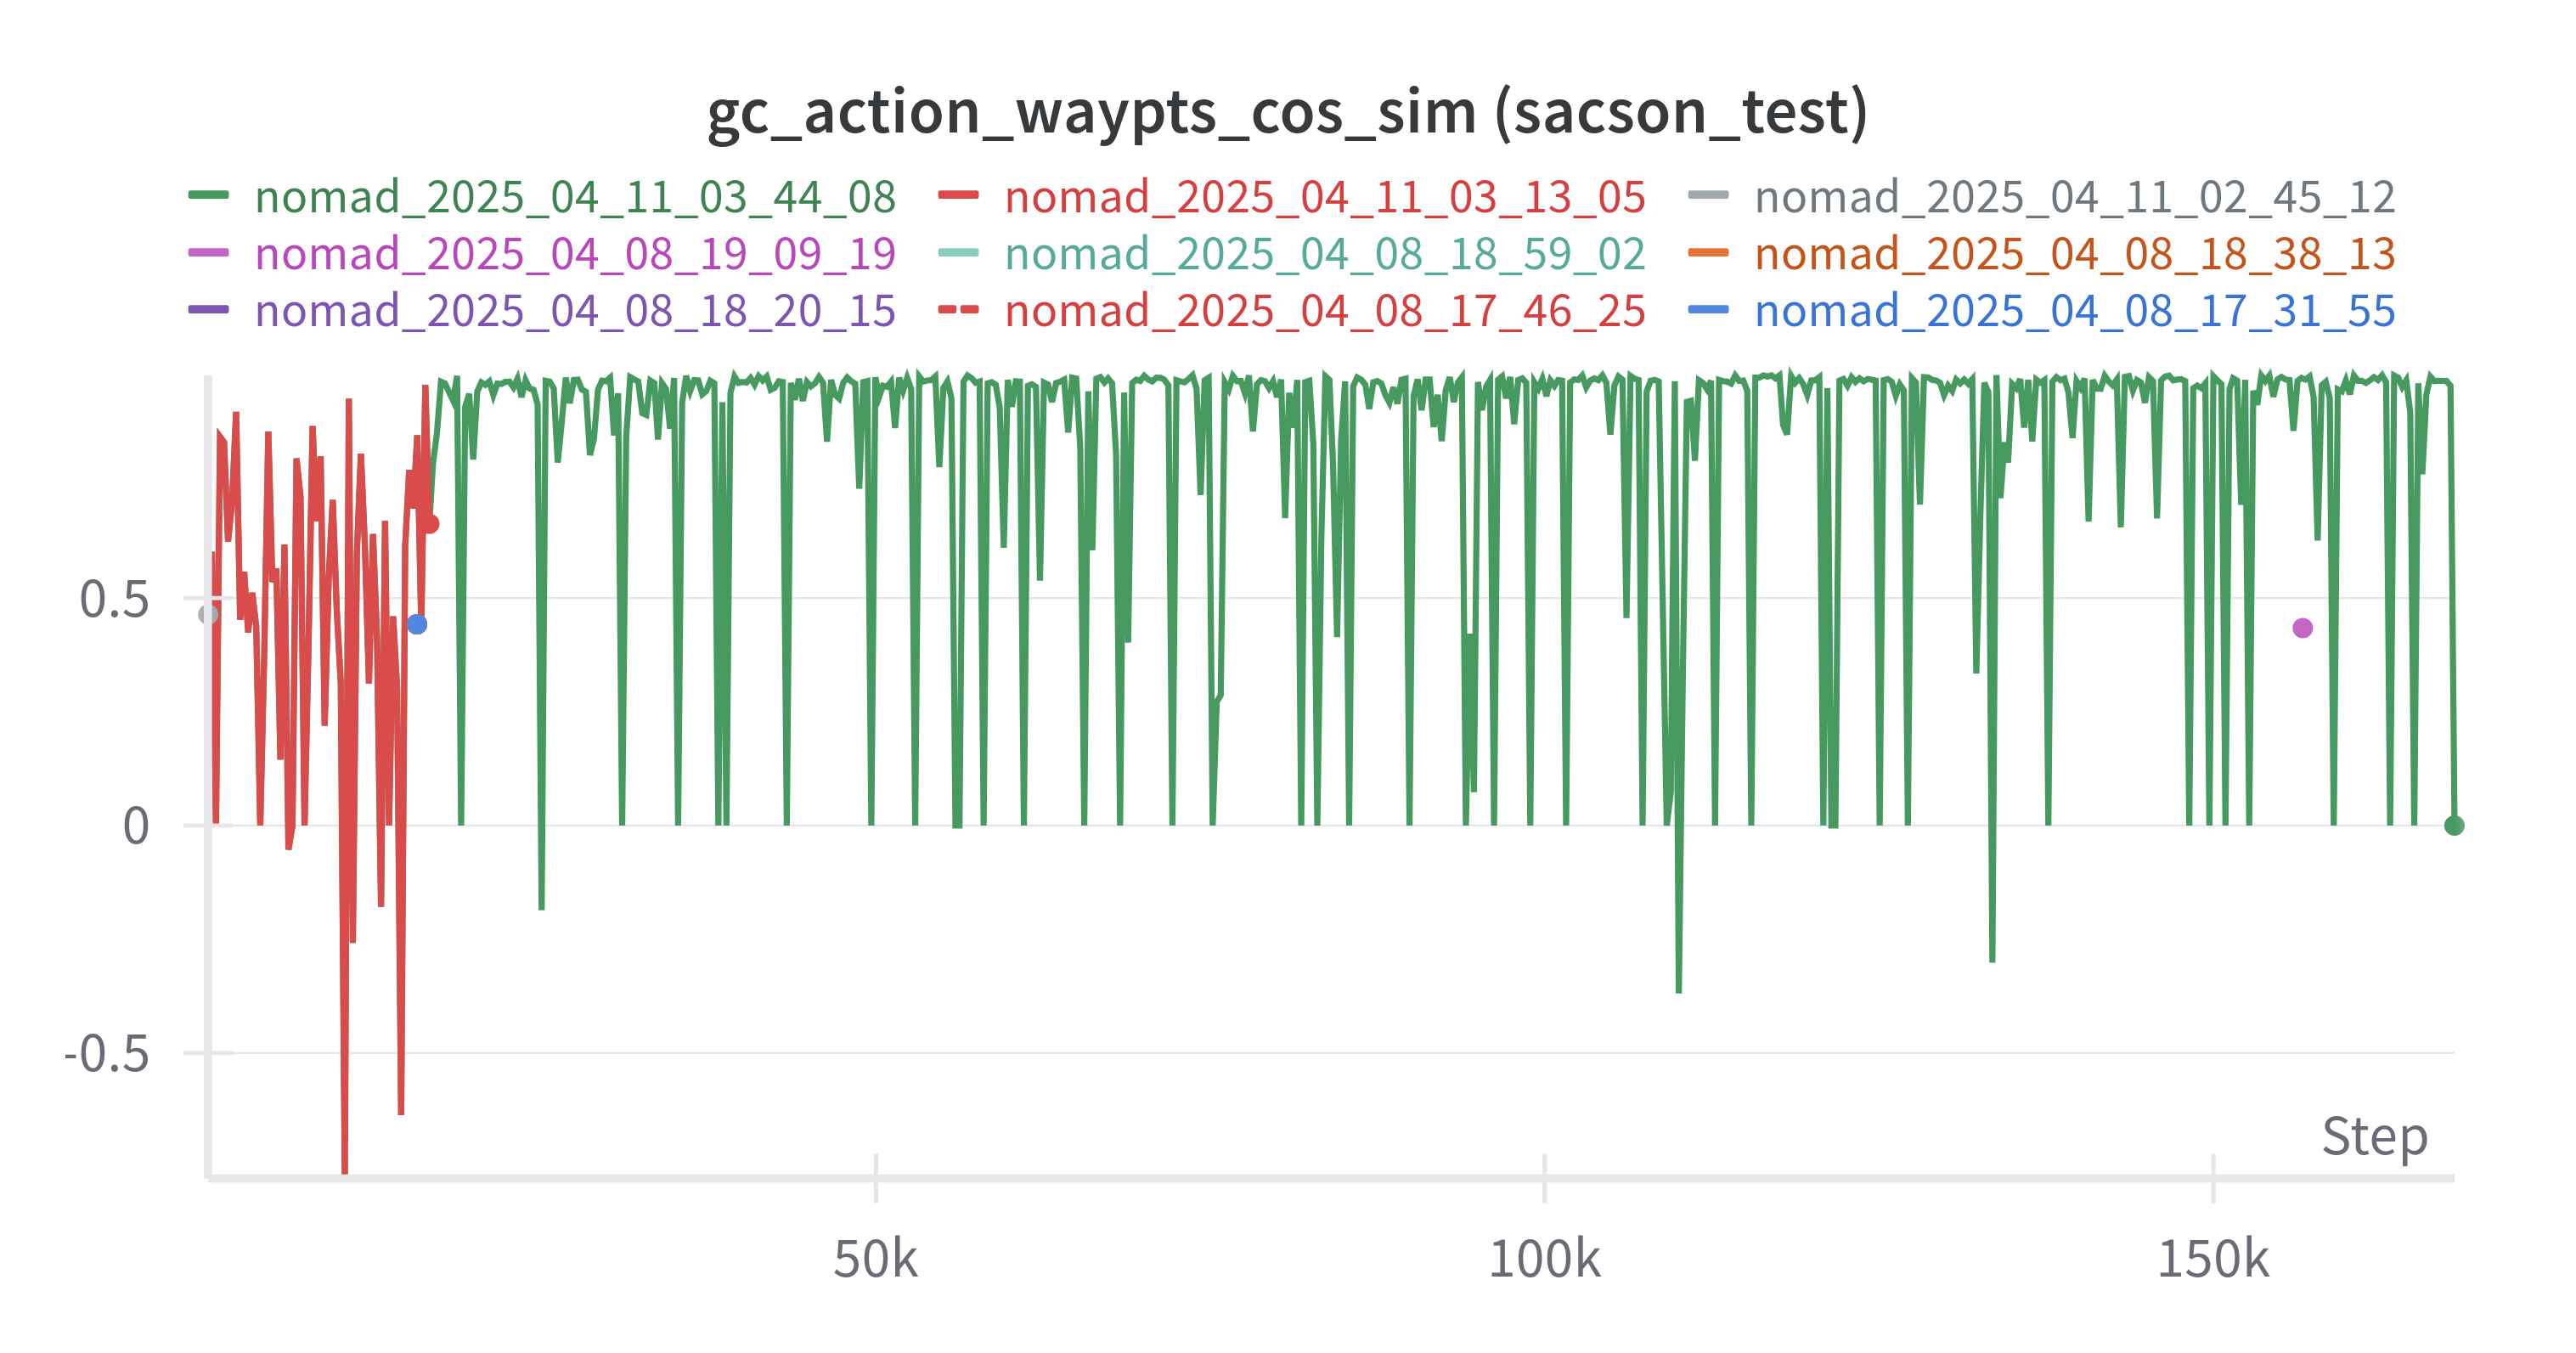
\includegraphics[width=\textwidth]{images/gc_action_cos_sim_test.png}
        \label{fig:action_test_nomad}
        \caption{NoMaD Action Cosine Similarity on Validation Set}
    \end{subfigure}
\end{figure}
\subsection*{Multi Action Cosine Similarity}
\begin{figure}[H]
    \centering
    \begin{subfigure}[b]{0.48\textwidth}
        \centering
        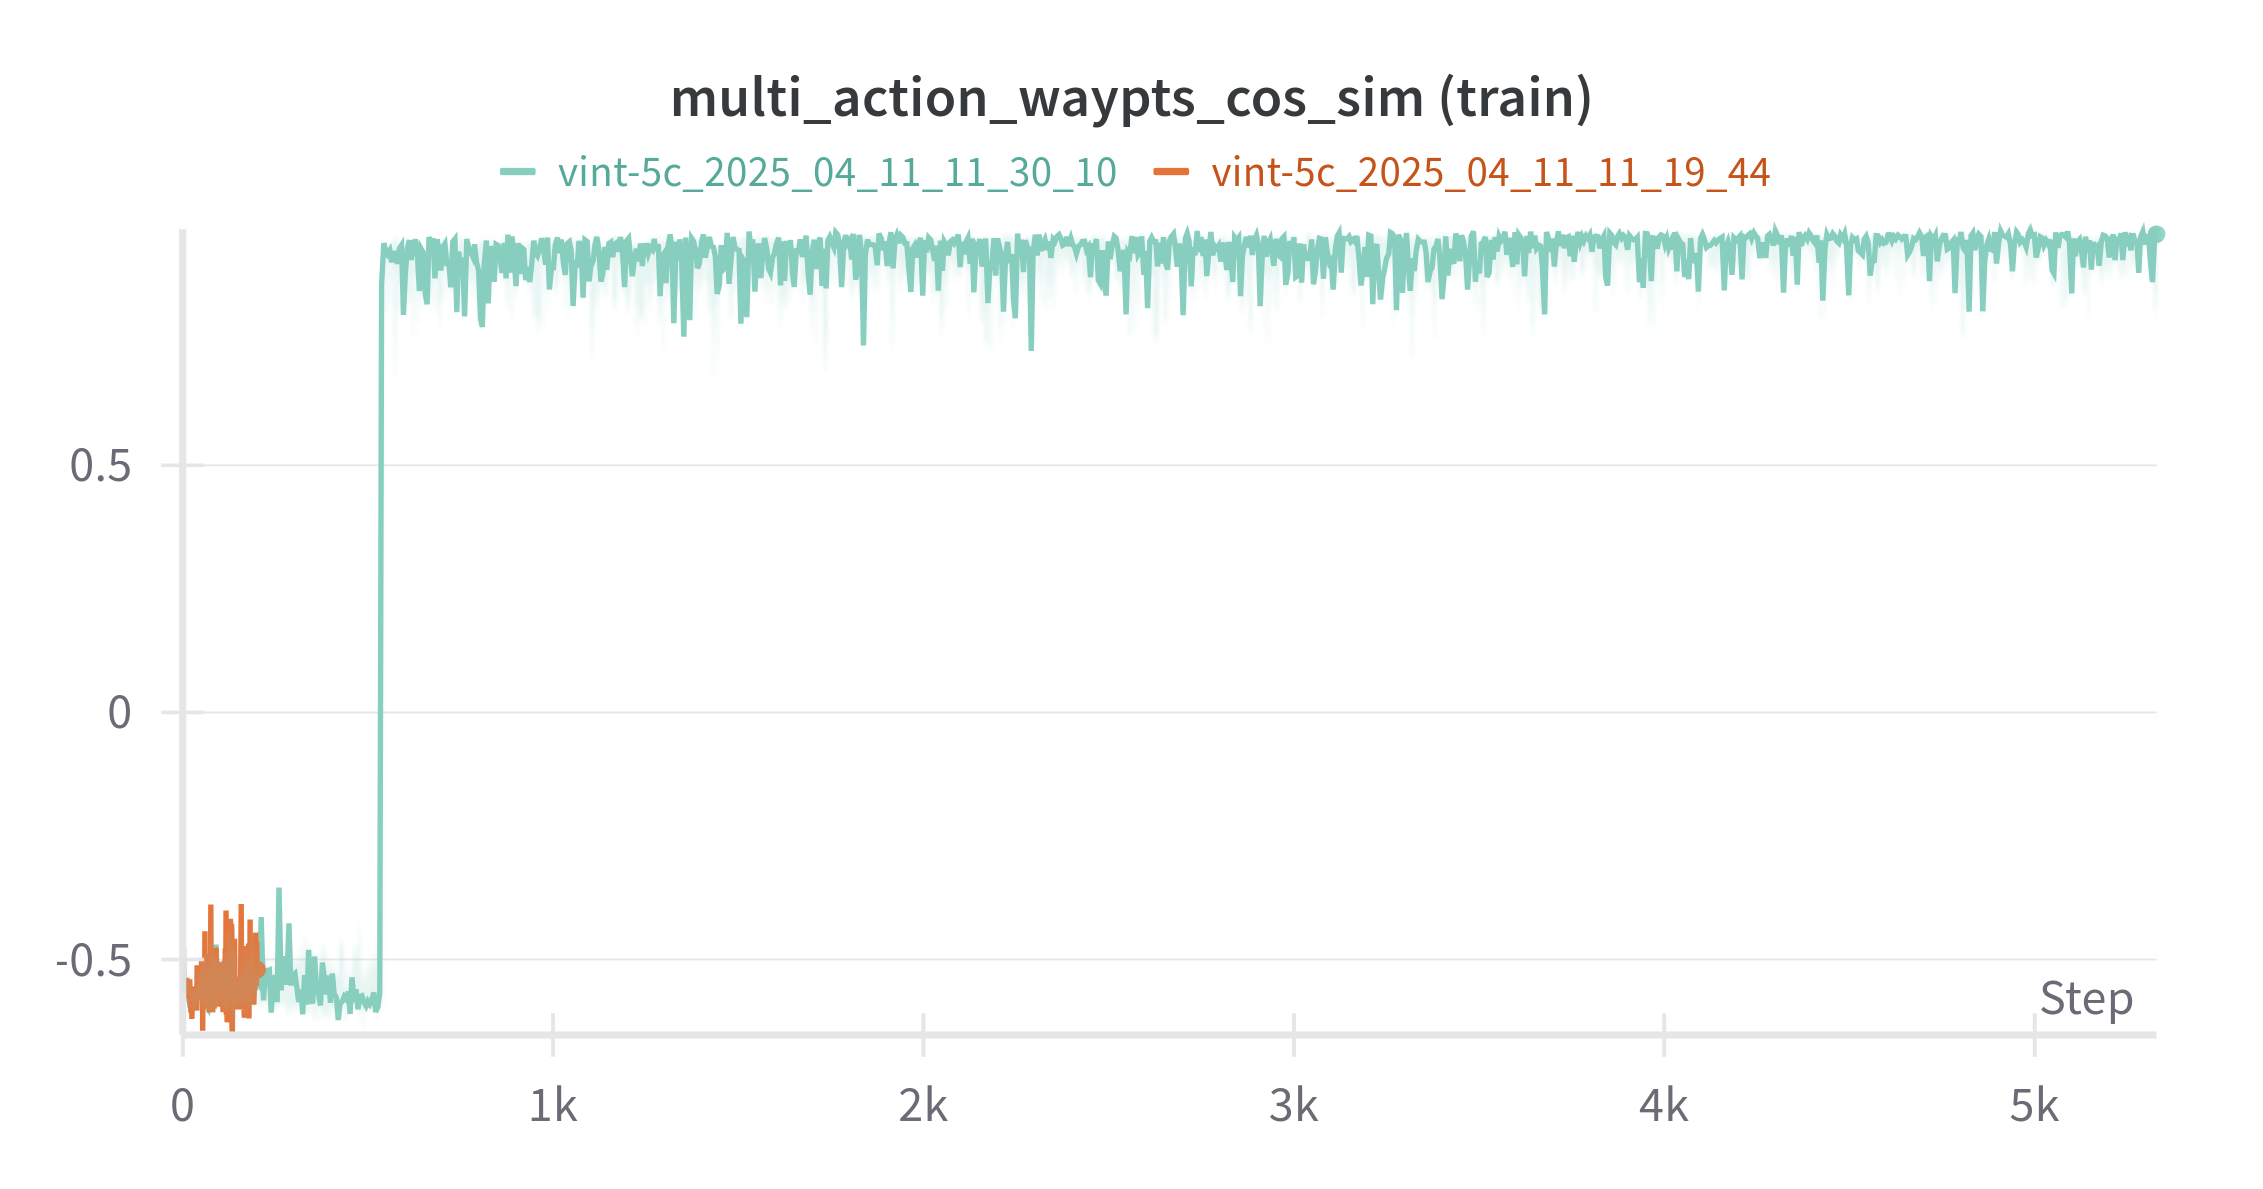
\includegraphics[width=\textwidth]{images/multiaction_train_vint.png}
        \label{fig:multiaction_train_vint}
        \caption{ViNT Multi Action Cosine Similarity on Training Set}
    \end{subfigure}
    \hfill
    \begin{subfigure}[b]{0.48\textwidth}
        \centering
        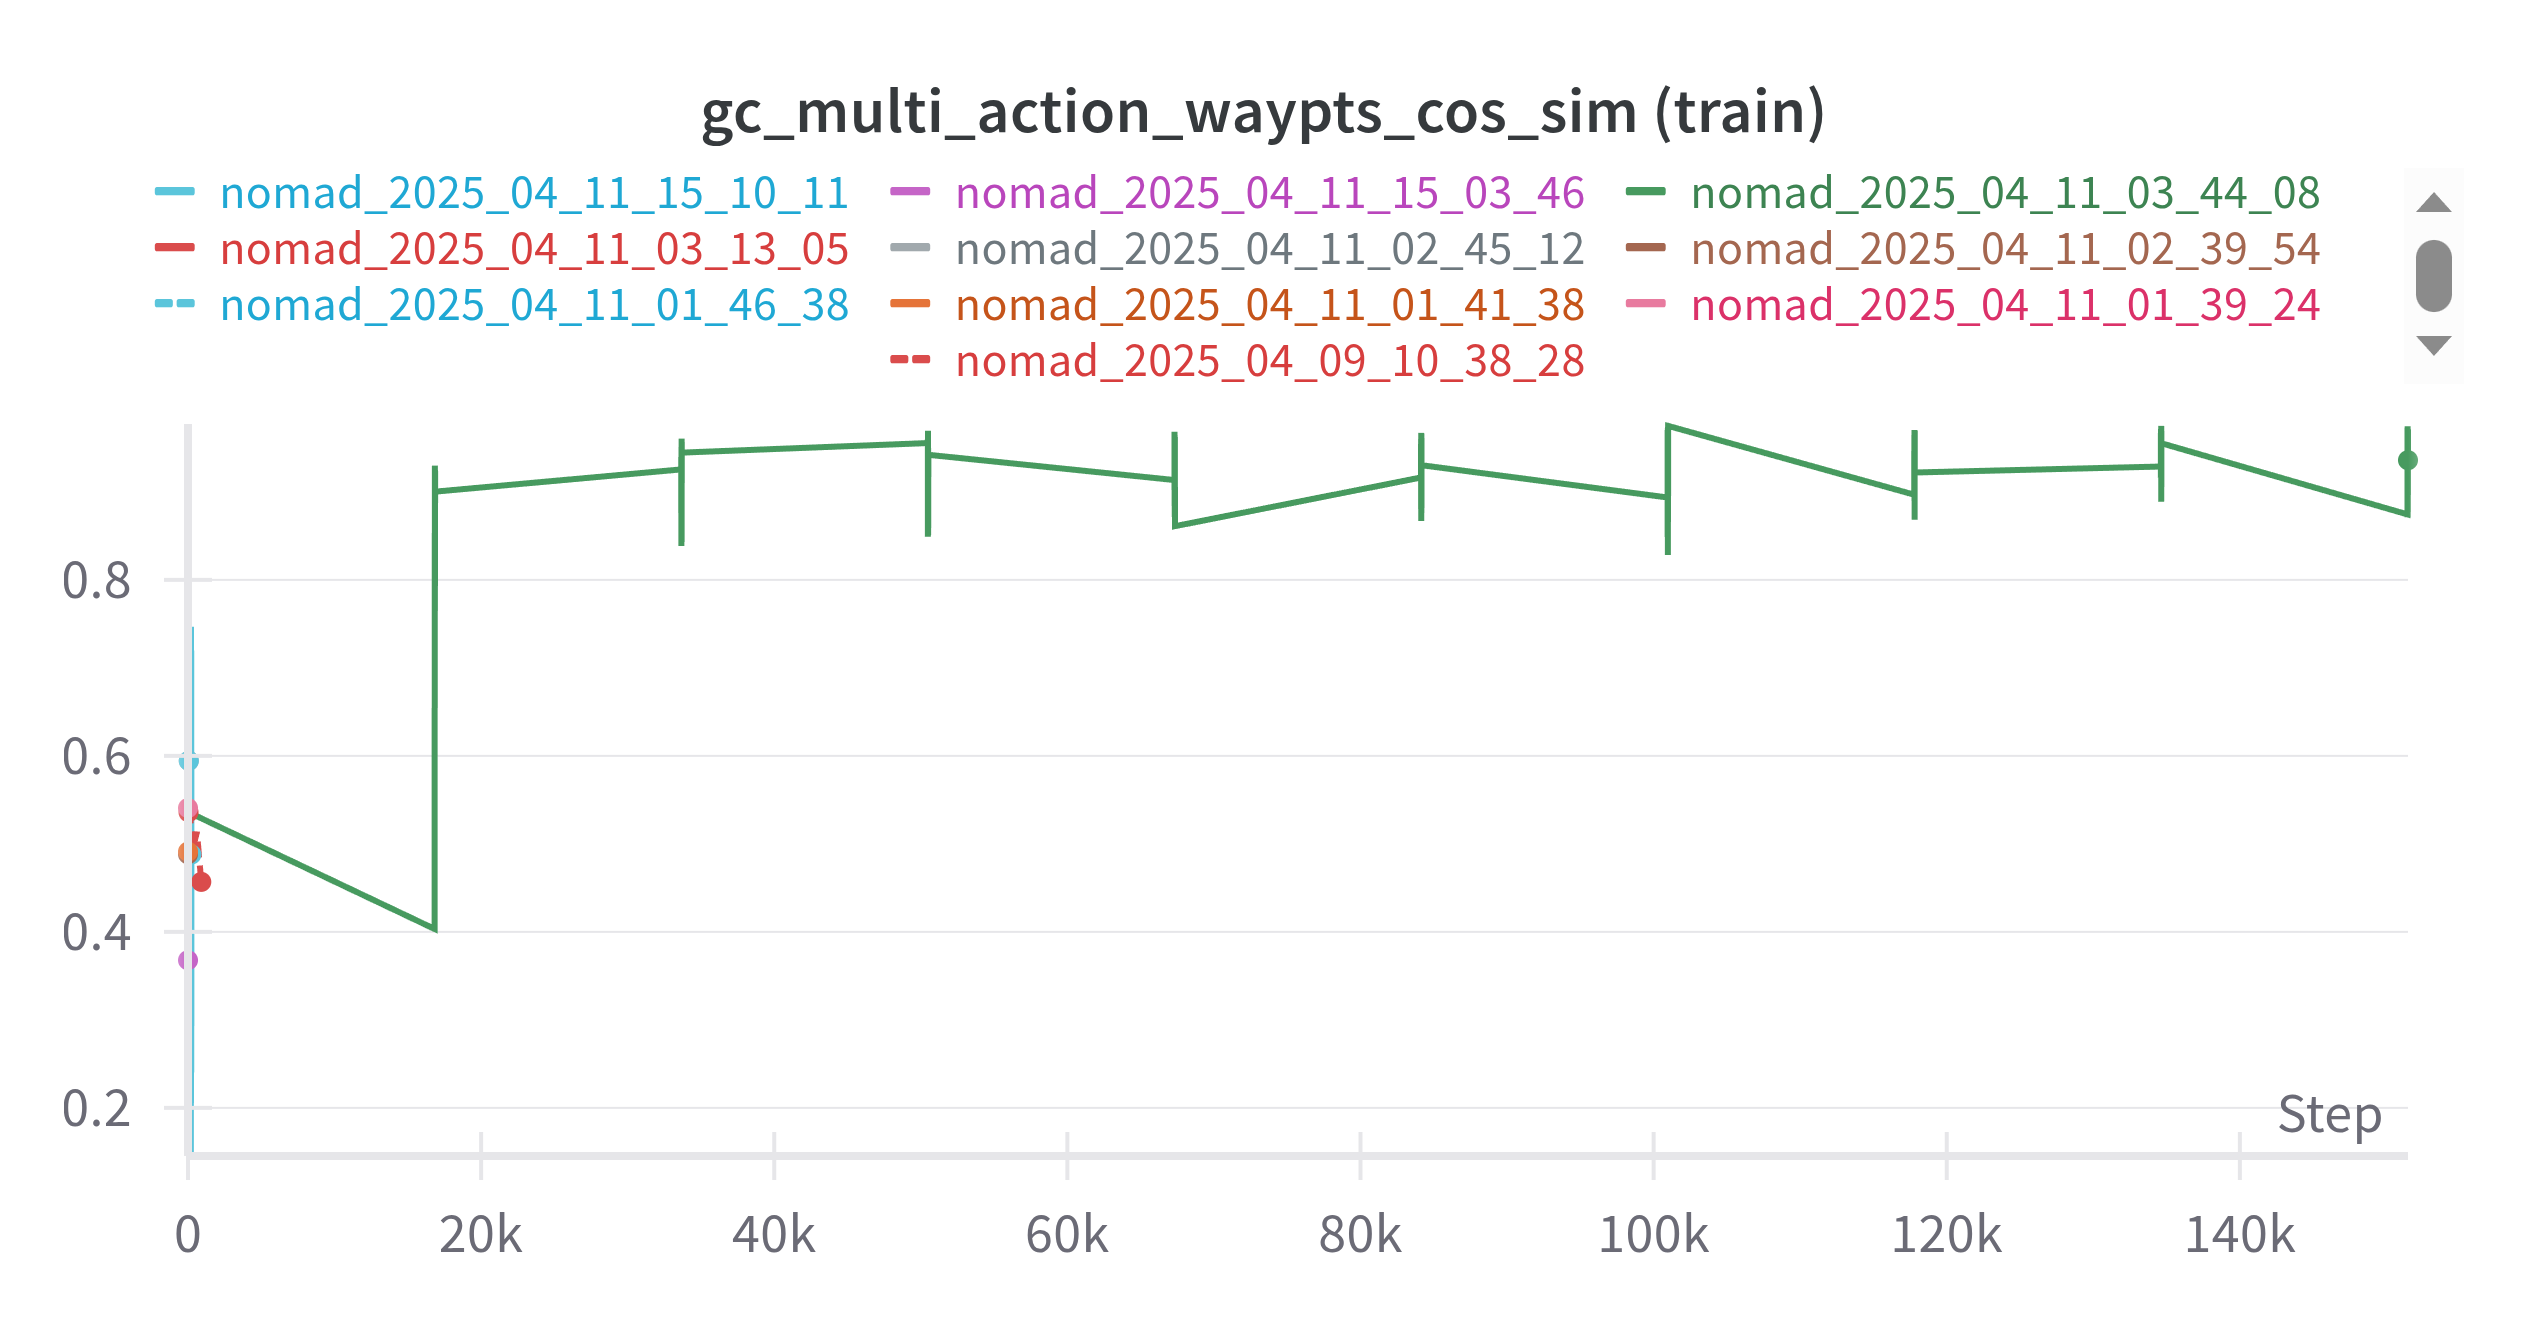
\includegraphics[width=\textwidth]{images/gc_multi_action_waypts_cos_sim.png}
        \label{fig:multiaction_train_nomad}
        \caption{NoMaD Multi Action Cosine Similarity on Training Set}
    \end{subfigure}
\end{figure}
\begin{figure}[H]
    \centering
    \begin{subfigure}[b]{0.48\textwidth}
        \centering
        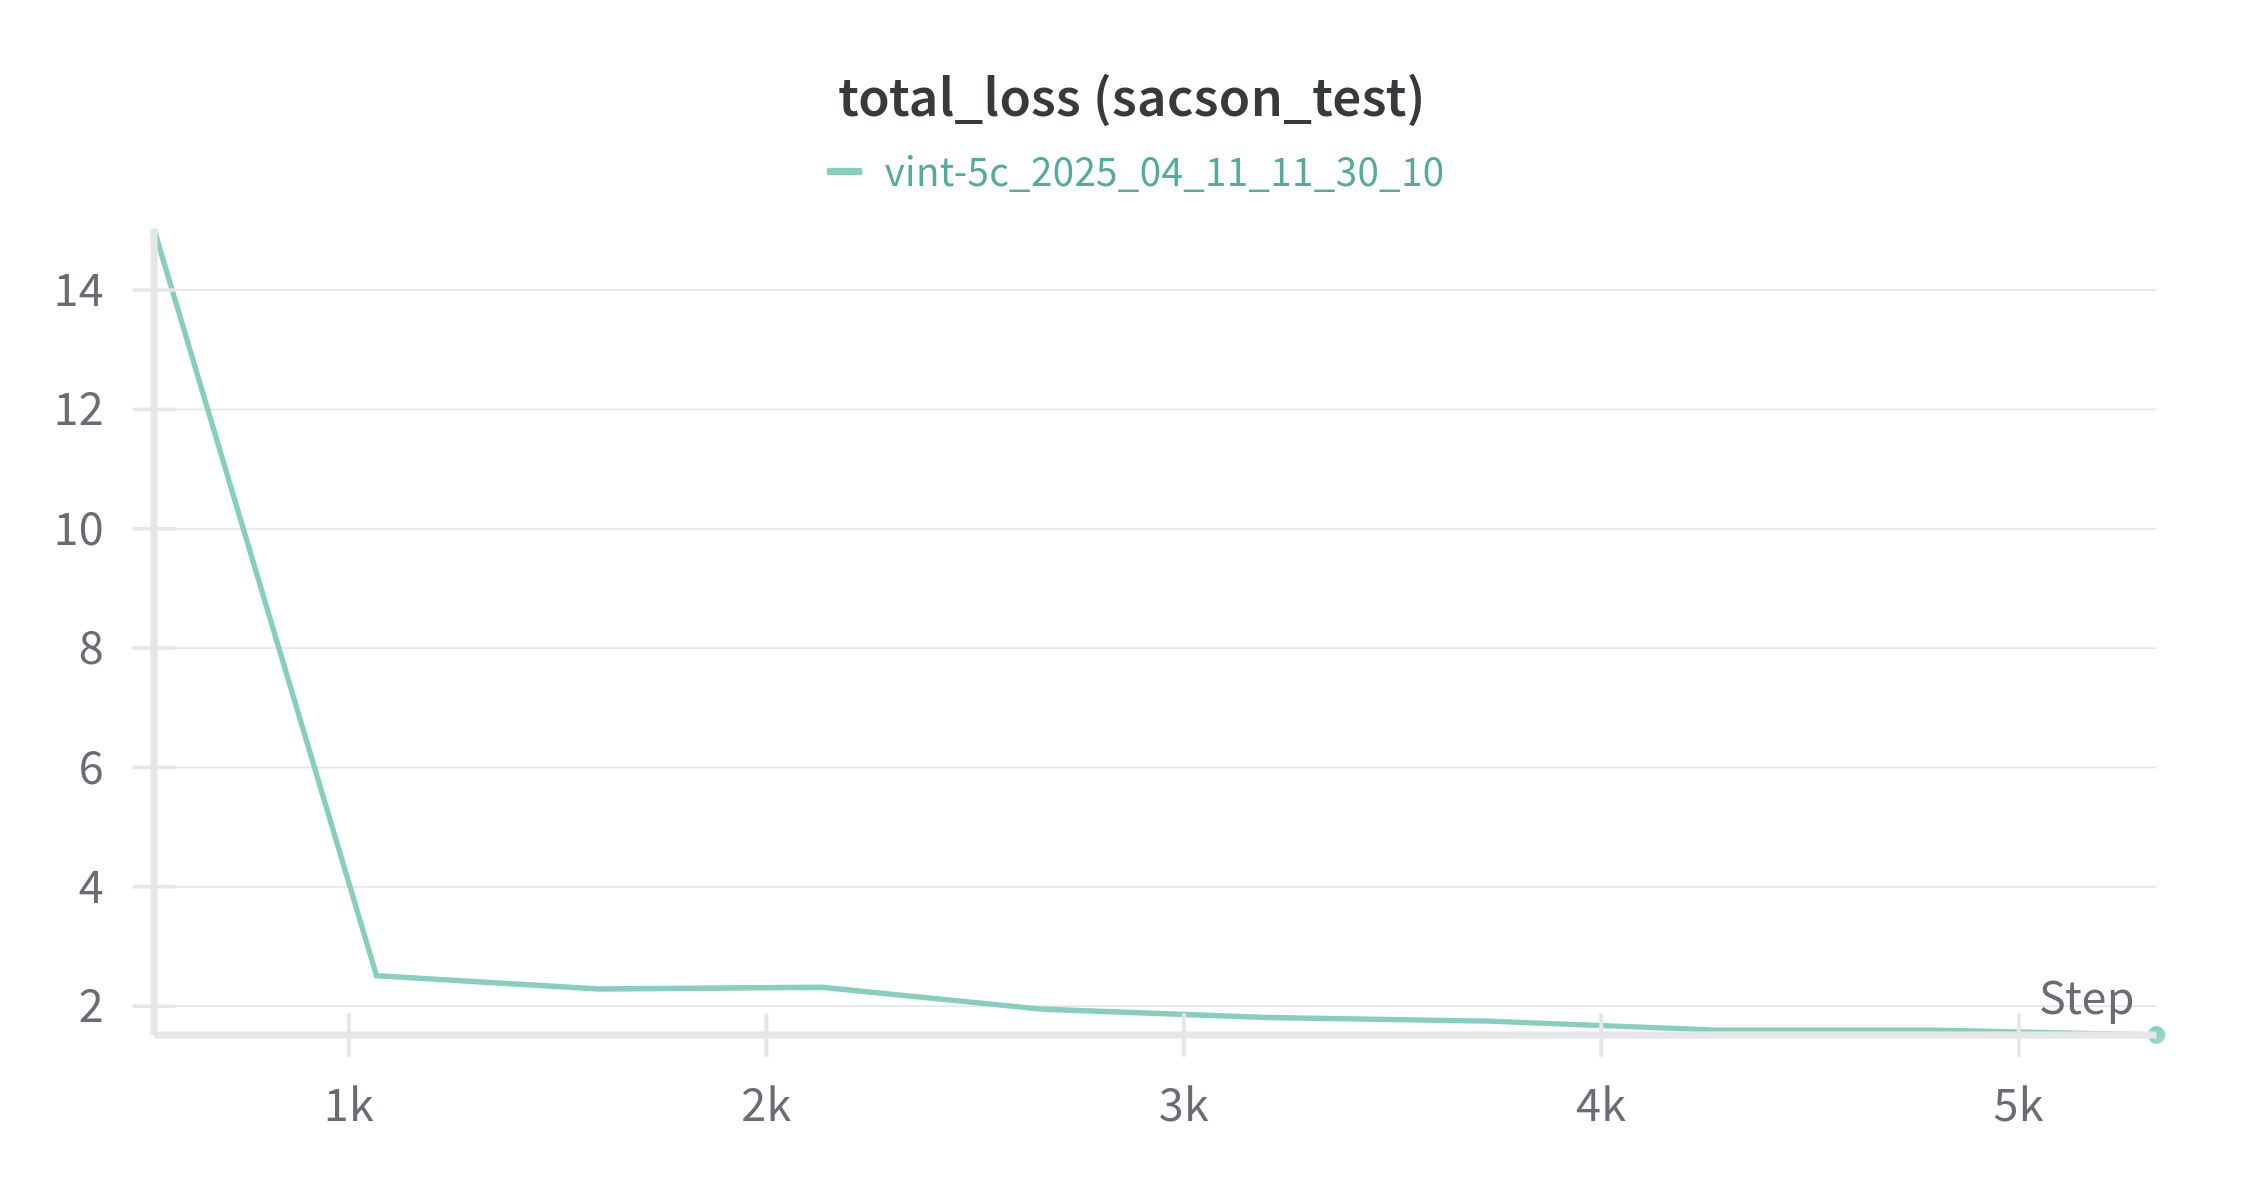
\includegraphics[width=\textwidth]{images/multiaction_test_vint.png}
        \label{fig:multiaction_test_vint}
        \caption{ViNT Multi Action Cosine Similarity on Validation Set}
    \end{subfigure}
    \hfill
    \begin{subfigure}[b]{0.48\textwidth}
        \centering
        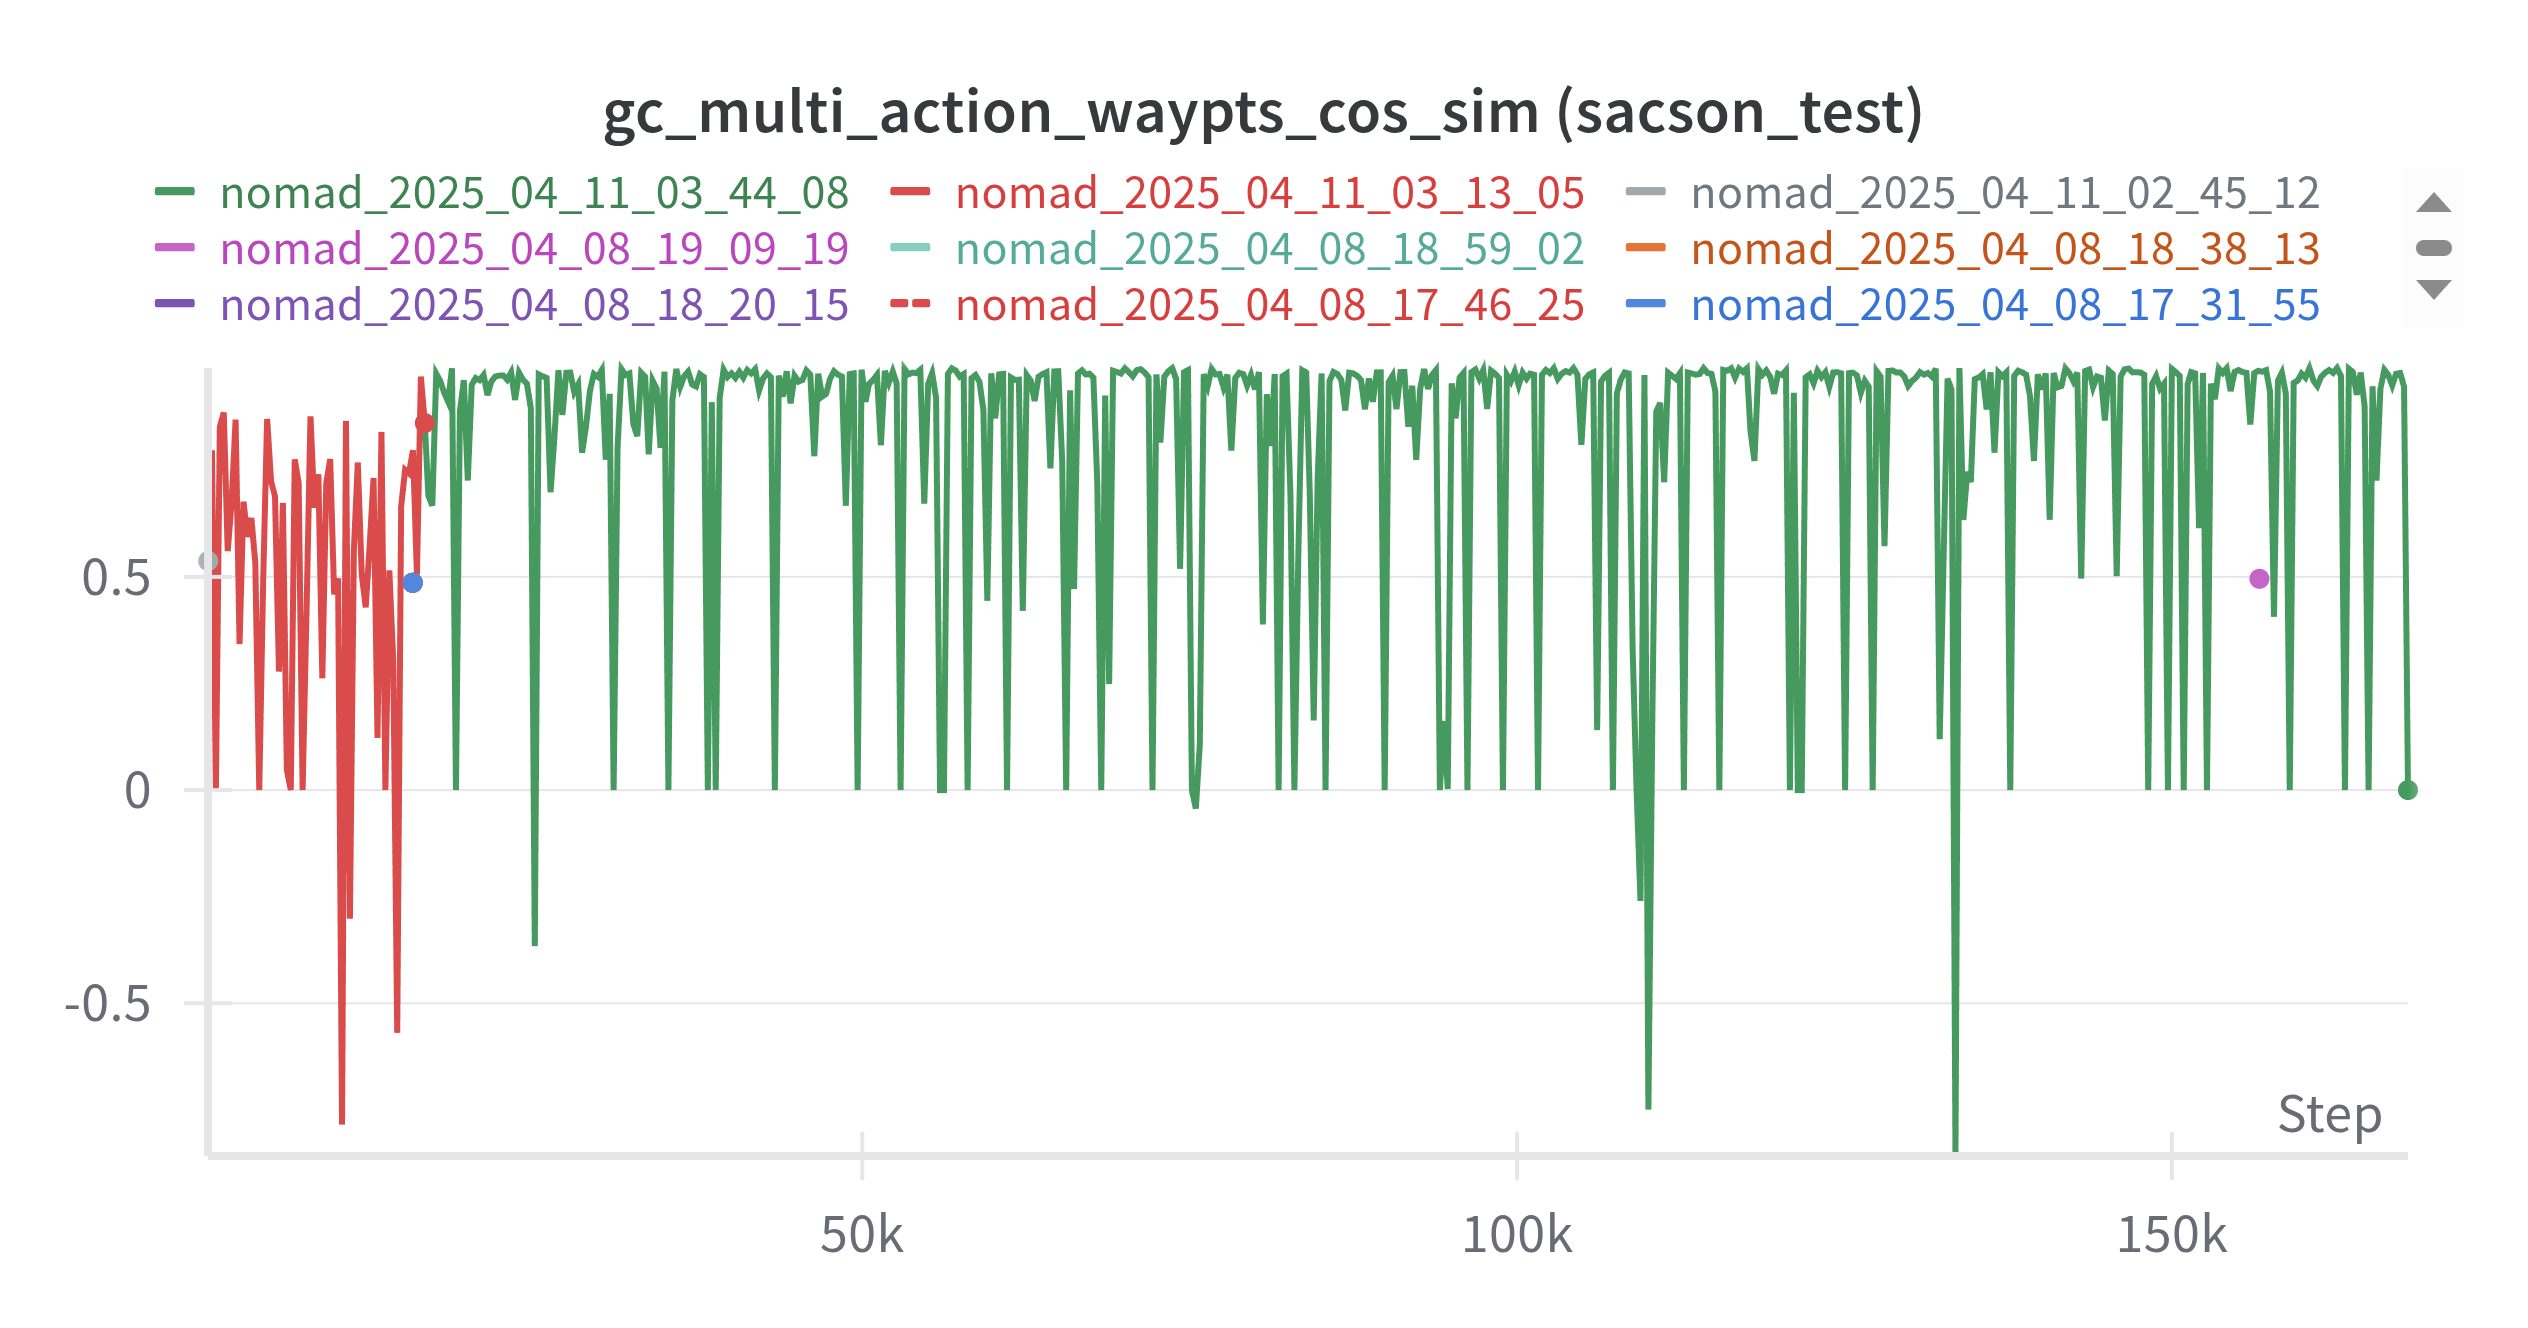
\includegraphics[width=\textwidth]{images/gc_multi_action_waypts_cos_sim_test.png}
        \label{fig:multiaction_test_nomad}
        \caption{NoMaD Multi Action Cosine Similarity on Validation Set}
    \end{subfigure}
\end{figure}
\newpage
Following are some of the visualizations of \textbf{ViNT} model's predictions on the validation set.\\
\begin{figure}[H]
    \centering
    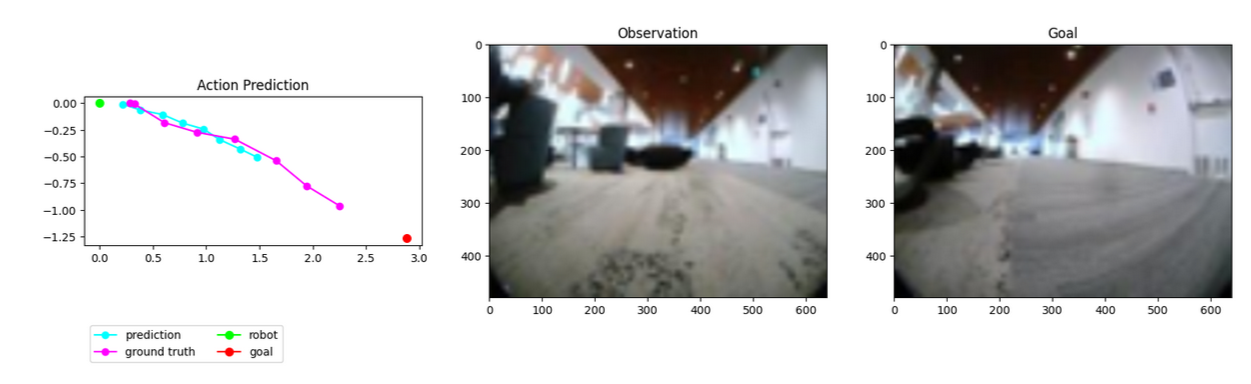
\includegraphics[width=\textwidth]{images/test_action_sample_vint.png}
    \label{fig:test_action_sample_vint}
\end{figure}
\begin{figure}[H]
    \centering
    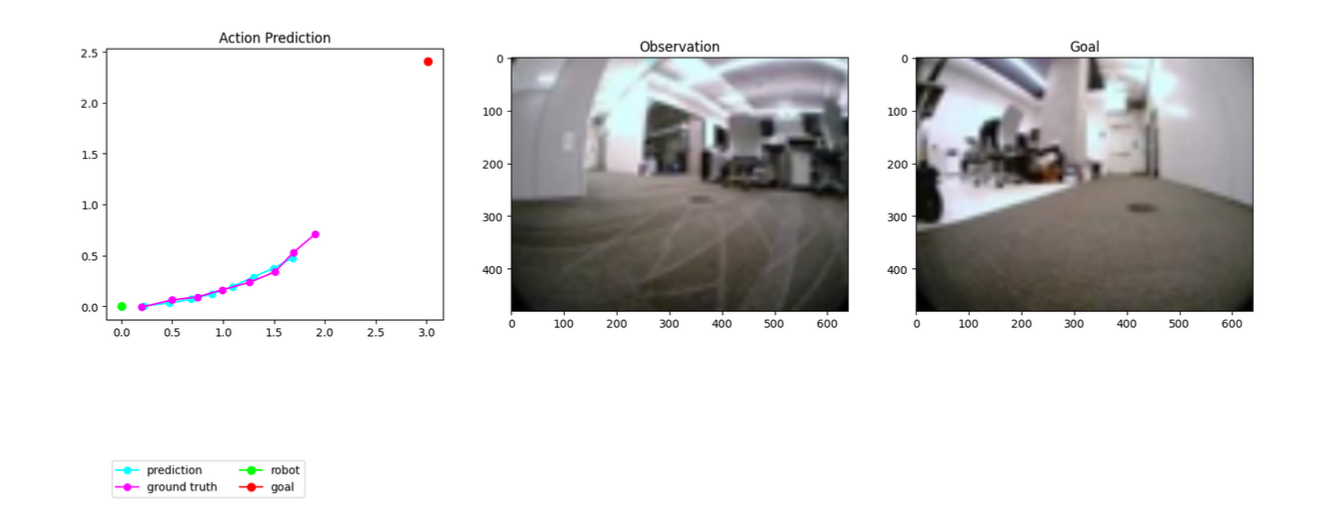
\includegraphics[width=\textwidth]{images/test_action_sample_vint_2.png}
    \label{fig:test_action_sample_vint2}
\end{figure}

\section{Vision Transformer (ViT)}
\label{app:vit}

\subsection*{1. Core Architecture}
ViT adapts the \textbf{Transformer} architecture, originally designed for NLP, to \textbf{image recognition} by treating images as sequences of patches.

\subsubsection*{(a) Patch Embedding}
An input image $\mathbf{X} \in \mathbf{R}^{H \times W \times C}$ is split into $N$ non-overlapping patches of size $P \times P$. Each patch is flattened into a 1D vector and linearly projected:

\[
\mathbf{z}_i = \mathbf{E} \mathbf{x}_i + \mathbf{b}
\]

where:
\begin{itemize}
    \item $\mathbf{x}_i \in \mathbf{R}^{P^2 \times C}$ is the flattened patch
    \item $\mathbf{E} \in \mathbf{R}^{D \times P^2 C}$ is the embedding matrix
    \item $D$ is the embedding dimension (e.g., 768)
\end{itemize}

For an image of size 224$\times$224 and patch size 16$\times$16:

\[
N = \left( \frac{224}{16} \right)^2 = 196 \text{ patches}
\]

\subsubsection*{(b) Class Token (CLS)}
A learnable classification token $\mathbf{z}_{cls} \in \mathbf{R}^D$ is prepended:

\[
\mathbf{Z} = [\mathbf{z}_{cls}; \mathbf{z}_1; \mathbf{z}_2; \dots; \mathbf{z}_N]
\]

\subsubsection*{(c) Positional Embeddings}
Learned positional embeddings are added to retain spatial information:

\[
\mathbf{Z} = \mathbf{Z} + \mathbf{E}_{pos}, \quad \mathbf{E}_{pos} \in \mathbf{R}^{(N+1) \times D}
\]

\subsection*{2. Transformer Encoder}
The ViT encoder consists of \textbf{L identical layers}, each containing:

\begin{itemize}
    \item Multi-Head Self-Attention (MHSA)
    \item Layer Normalization (LN)
    \item Feed-Forward Network (FFN)
    \item Residual Connections
\end{itemize}

\subsubsection*{(a) Multi-Head Self-Attention (MHSA)}
Input embeddings are split into $h$ heads (e.g., 12 heads for ViT-Base). For each head:

\[
\text{Attention}(\mathbf{Q}, \mathbf{K}, \mathbf{V}) = \text{softmax}\left( \frac{\mathbf{Q} \mathbf{K}^T}{\sqrt{d_k}} \right) \mathbf{V}
\]

where $d_k = D / h$.

\subsubsection*{(b) Feed-Forward Network (FFN)}
A 2-layer MLP with GELU activation:

\[
\text{FFN}(\mathbf{x}) = \mathbf{W}_2 \text{GELU}(\mathbf{W}_1 \mathbf{x} + \mathbf{b}_1) + \mathbf{b}_2
\]

where:
\begin{itemize}
    \item $\mathbf{W}_1 \in \mathbf{R}^{4D \times D}$
    \item $\mathbf{W}_2 \in \mathbf{R}^{D \times 4D}$
\end{itemize}

\subsubsection*{(c) Layer Normalization \& Residual Connections}
Each sub-layer is wrapped with:

\[
\mathbf{x}_{\text{out}} = \text{LayerNorm}(\mathbf{x} + \text{SubLayer}(\mathbf{x}))
\]

\subsection*{3. Training \& Fine-Tuning}
\begin{itemize}
    \item \textbf{Pre-training}: On large datasets (e.g., JFT-300M)
    \item \textbf{Fine-tuning}: Adapt to downstream tasks by replacing classification head
\end{itemize}

\section{EfficientNet}
\label{app:efficientnet}
\subsection*{1. Compound Scaling}
EfficientNet introduces \textbf{compound scaling}:

\[
d = \alpha^\phi, \quad w = \beta^\phi, \quad r = \gamma^\phi
\]

where:
\begin{itemize}
    \item $\phi$ is a scaling coefficient
    \item $\alpha, \beta, \gamma$ are constants ($\alpha = 1.2, \beta = 1.1, \gamma = 1.15$)
\end{itemize}

\textbf{Constraint}:
\[
\alpha \cdot \beta^2 \cdot \gamma^2 \approx 2
\]

\subsection*{2. MBConv Block}
The core building block consists of:
\begin{itemize}
    \item 1×1 Expansion Conv (expansion factor $t=6$)
    \item Depthwise Conv
    \item Squeeze-and-Excitation (SE) Block
    \item 1×1 Projection Conv
\end{itemize}

\subsubsection*{(a) Depthwise Separable Convolution}
\begin{itemize}
    \item \textbf{Depthwise Conv}:
    \[
    \mathbf{y}_{i,j,k} = \sum_{m,n} \mathbf{K}_{m,n,k} \mathbf{x}_{i+m, j+n, k}
    \]
    \item \textbf{Pointwise Conv}:
    \[
    \mathbf{z}_{i,j,l} = \sum_k \mathbf{W}_{k,l} \mathbf{y}_{i,j,k}
    \]
\end{itemize}

\subsubsection*{(b) Squeeze-and-Excitation (SE)}
\begin{itemize}
    \item \textbf{Squeeze}: Global average pooling $\rightarrow \mathbf{s} \in \mathbf{R}^C$
    \item \textbf{Excitation}:
    \[
    \mathbf{s}_{excite} = \sigma(\mathbf{W}_2 \text{ReLU}(\mathbf{W}_1 \mathbf{s}))
    \]
    \item \textbf{Rescale}:
    \[
    \mathbf{x}_{out} = \mathbf{s}_{excite} \odot \mathbf{x}
    \]
\end{itemize}

\subsection*{3. Neural Architecture Search (NAS)}
EfficientNet-B0 was discovered using:

\[
\text{maximize } \text{ACC}(m) \times \left[ \frac{\text{FLOPS}(m)}{T} \right]^w
\]

where:
\begin{itemize}
    \item $w = -0.07$
    \item $T = 400M$ (target FLOPS for B0)
\end{itemize}

\section{Diffusion Policy: Visuomotor Policy Learning via Action Diffusion} \cite{diff_paper}
\label{app:diffusion}
\textbf{Diffusion Policy}, a novel approach for generating robot behavior by representing a robot's visuomotor policy as a conditional denoising diffusion process. This method leverages the strengths of diffusion models to address challenges in robot policy learning, such as handling multimodal action distributions, high-dimensional action spaces, and training stability. The authors benchmark Diffusion Policy across 15 tasks from 4 different robot manipulation benchmarks, demonstrating an average improvement of 46.9\% over existing state-of-the-art methods.\\
Traditional policy learning from demonstrations faces challenges due to:
\begin{itemize}
    \item \textbf{Multimodal action distributions}: Multiple valid actions for the same observation.
    \item \textbf{Sequential correlation}: Actions are temporally dependent.
    \item \textbf{High precision requirements}: Robot tasks often require precise control.
\end{itemize}

Prior work has explored various action representations (e.g., mixtures of Gaussians, categorical representations) and policy representations (e.g., explicit vs. implicit policies). However, these methods often struggle with stability, scalability, or expressiveness.

\subsection*{Diffusion Policy Formulation}
Diffusion Policy is based on Denoising Diffusion Probabilistic Models (DDPMs), adapted for robot visuomotor control. The key modifications include:
\begin{itemize}
    \item \textbf{Action-space diffusion}: The output \(\mathbf{x}\) represents robot actions instead of images.
    \item \textbf{Conditional denoising}: The denoising process is conditioned on input observations \(\mathbf{O}_t\).
\end{itemize}

The policy predicts action sequences using a receding horizon control strategy:
\begin{itemize}
    \item At time \(t\), the policy takes the latest \(T_o\) steps of observations and predicts \(T_p\) steps of actions.
    \item Only \(T_a\) steps are executed before re-planning, balancing temporal consistency and responsiveness.
\end{itemize}

\subsubsection*{Training}
The training process involves:
\begin{enumerate}
    \item Sampling an action \(\mathbf{A}_t^0\) from the dataset.
    \item Adding noise \(\boldsymbol{\varepsilon}^k\) to create a noisy action \(\mathbf{A}_t^k\).
    \item Training the noise prediction network \(\epsilon_\theta\) to estimate \(\boldsymbol{\varepsilon}^k\) given \(\mathbf{O}_t\) and \(\mathbf{A}_t^k\).
\end{enumerate}

The loss function is:
\[
\mathcal{L} = \text{MSE}(\boldsymbol{\varepsilon}^k, \epsilon_\theta(\mathbf{O}_t, \mathbf{A}_t^0 + \boldsymbol{\varepsilon}^k, k)).
\]

\subsection*{Network Architectures}
Two architectures are explored:
\begin{itemize}
    \item \textbf{CNN-based}: Uses 1D temporal CNNs with FiLM conditioning for observation features. Suitable for most tasks but struggles with high-frequency action changes.
    \item \textbf{Transformer-based}: Introduces a time-series diffusion transformer to reduce over-smoothing. Performs better for complex tasks but requires more tuning.
\end{itemize}

\subsection*{Visual Conditioning}
Visual observations are encoded independently for each timestep and concatenated into a latent embedding \(\mathbf{O}_t\). A ResNet-18 encoder is used with modifications:
\begin{itemize}
    \item Spatial softmax pooling replaces global average pooling.
    \item GroupNorm replaces BatchNorm for stable training.
\end{itemize}

\subsection*{Noise Schedule}
The square cosine schedule from iDDPM is used to control the noise level during denoising, balancing high- and low-frequency action characteristics.

\subsection*{Inference Acceleration}
Denoising Diffusion Implicit Models (DDIM) reduce inference iterations from 100 to 16, enabling real-time control with low latency (0.1s on an NVIDIA 3080 GPU).


\subsection*{Multimodal Action Distributions}
Diffusion Policy naturally handles multimodal action distributions by:
\begin{itemize}
    \item Stochastic initialization: Starting from random noise allows exploration of different modes.
    \item Stochastic optimization: Gaussian perturbations during denoising enable transitions between modes.
\end{itemize}
The method scales well to high-dimensional action spaces, enabling joint prediction of action sequences for long-horizon planning.
Unlike implicit policies that require negative sampling, Diffusion Policy learns the score function directly, avoiding instability issues.
Diffusion Policy performs better with position control than velocity control, contrasting with prior work that favors velocity control.\\
The authors evaluate Diffusion Policy on 15 tasks across 4 benchmarks:
\begin{itemize}
    \item \textbf{Robomimic}: 5 manipulation tasks with human demonstrations.
    \item \textbf{Push-T}: A planar pushing task with RGB or keypoint observations.
    \item \textbf{Multimodal Block Pushing}: Tests long-horizon multimodality.
    \item \textbf{Franka Kitchen}: A multi-task environment with 7 objects.
\end{itemize}

\subsubsection*{Key Findings}
\begin{itemize}
    \item Diffusion Policy outperforms baselines (LSTM-GMM, IBC, BET) by 46.9\% on average.
    \item Handles both short- and long-horizon multimodality effectively.
    \item Stable training with consistent hyperparameters across tasks.
\end{itemize}
\newpage
\section{WandB}
\label{app:wandb}
These are our initial plots of \texttt{distance\_loss}, \texttt{diffusion\_loss} and \texttt{total\_loss}.
\begin{figure}[H]
    \centering
    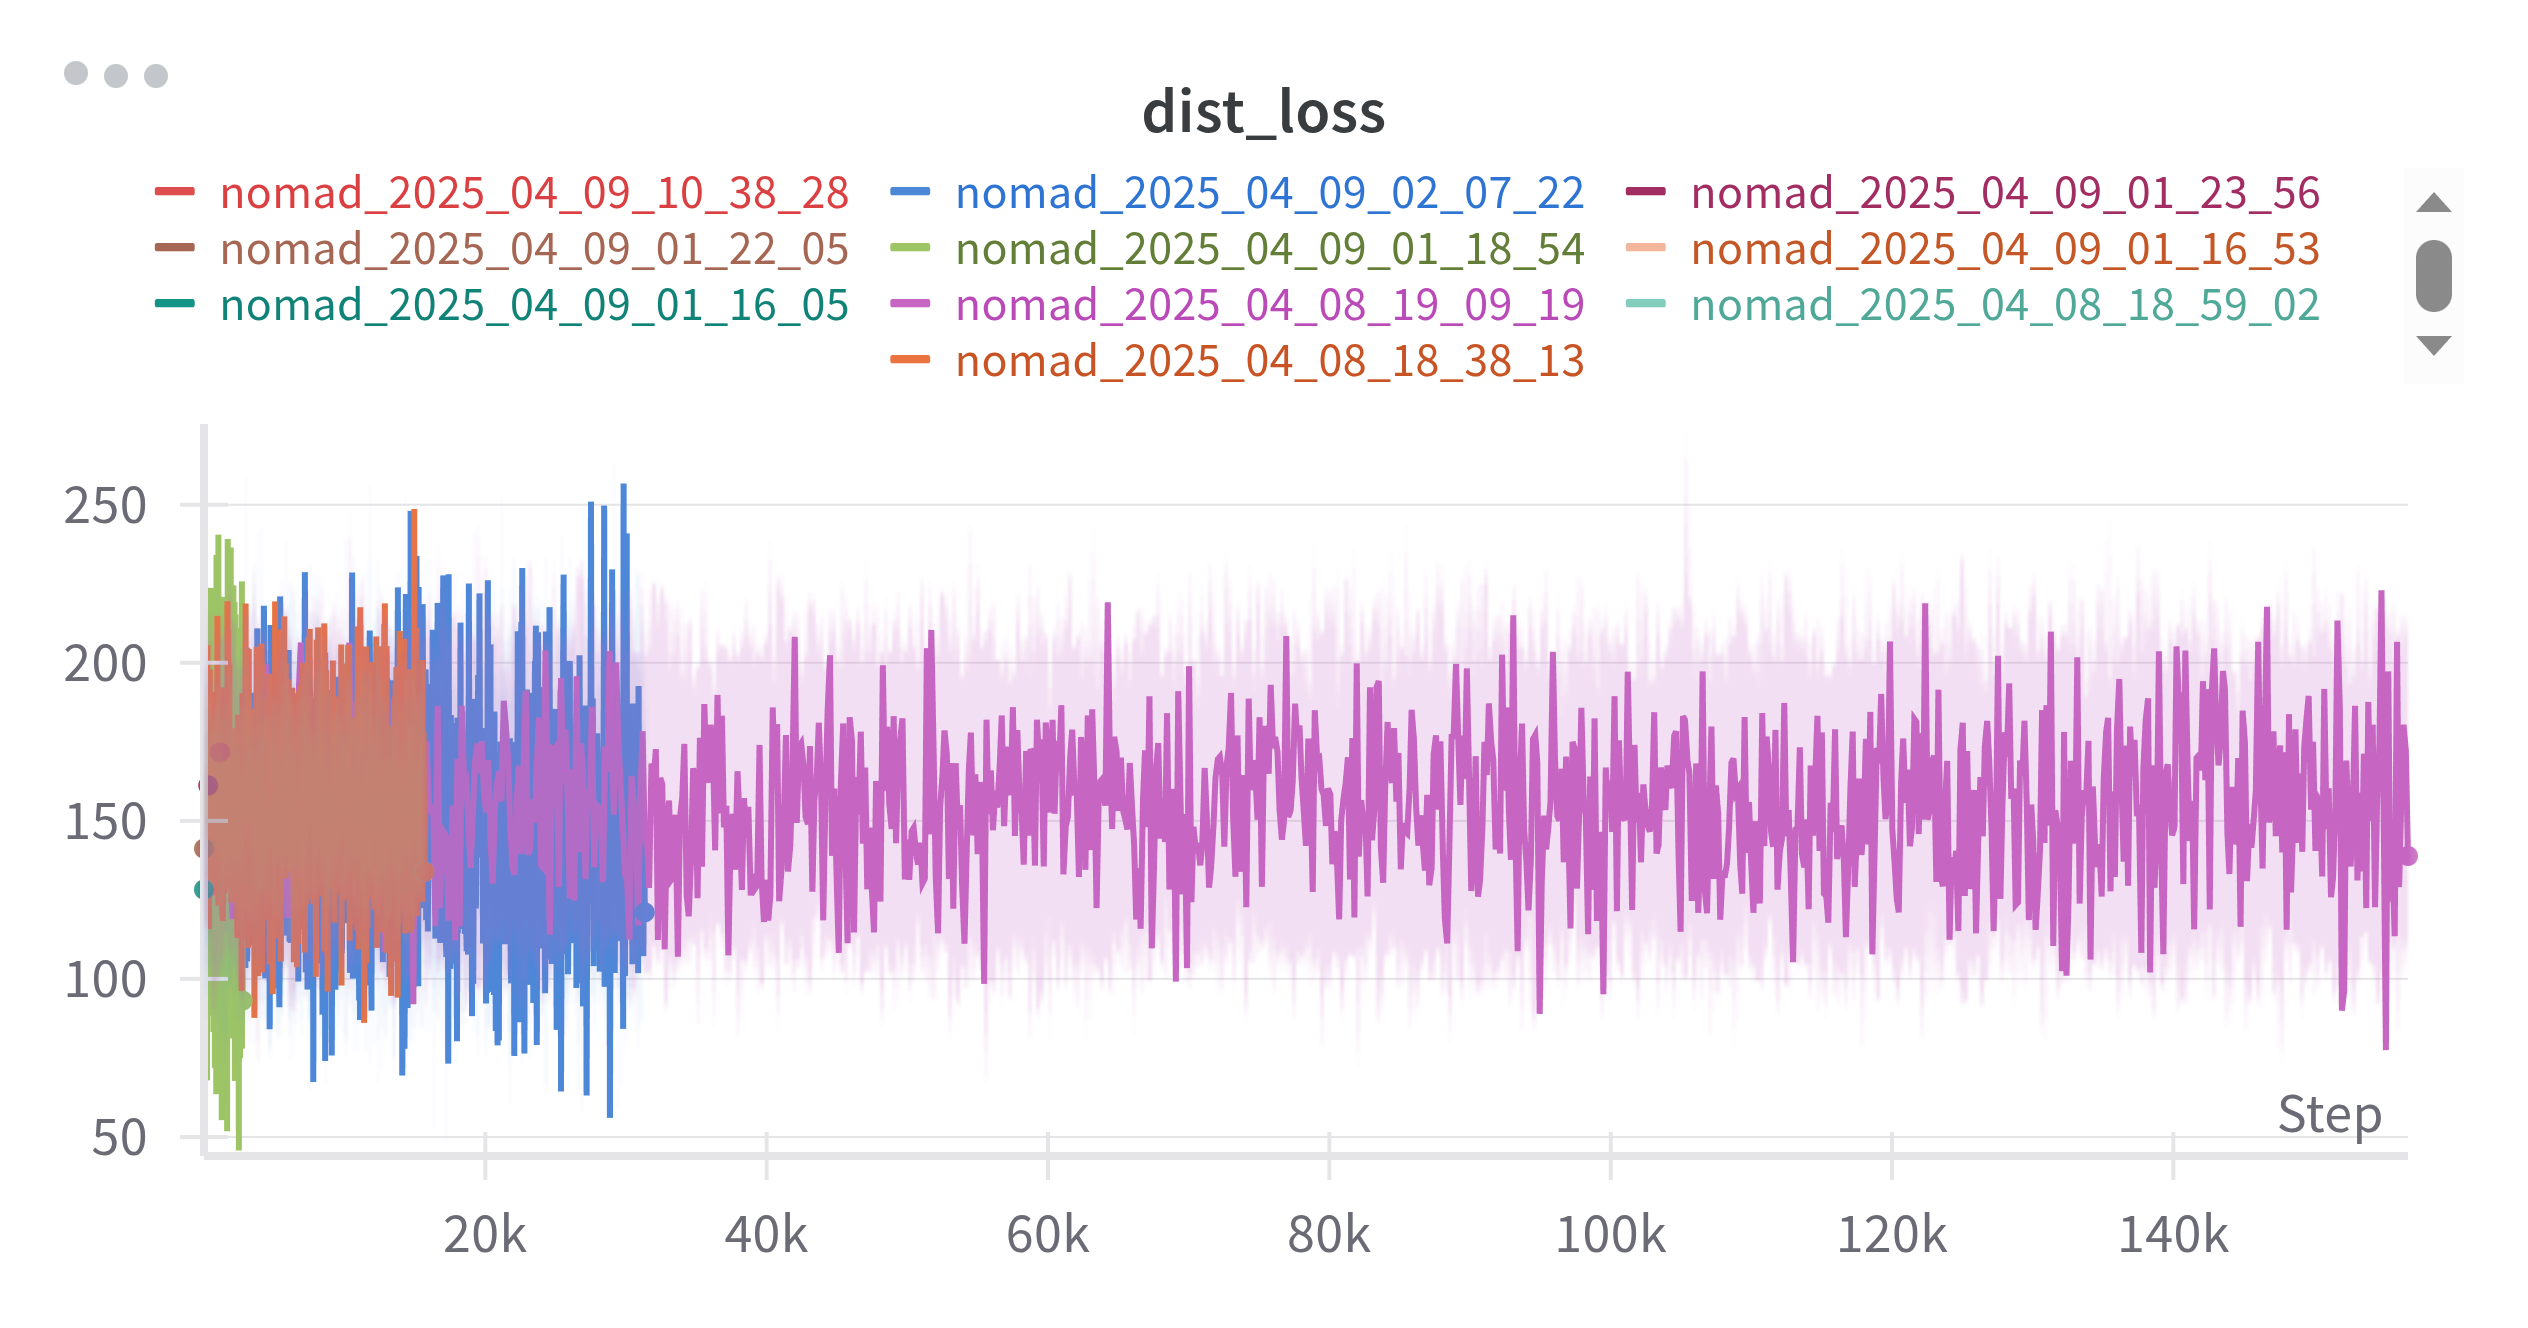
\includegraphics[width=\textwidth]{images/old_dist_loss.png}
    \caption{Initial plot of distance Loss on Training Set}
    \label{fig:init_dist_loss}
\end{figure}
\begin{figure}[H]
    \centering
    \includegraphics[width=\textwidth]{images/diffloss.png}
    \caption{Initial plot of diffusion Loss on Training Set}
    \label{fig:init_diff_loss}
\end{figure}
\begin{figure}[H]
    \centering
    \includegraphics[width=\textwidth]{images/totalloss_nomad.png}
    \caption{Initial plot of total Loss on Training Set}
    \label{fig:init_total_loss}
\end{figure}
It is somewhat surprising that the total distance\ref{fig:init_dist_loss}, diffusion losses \ref{fig:init_diff_loss} as well as total loss \ref{fig:init_total_loss} do not show the expected downward trend. However, other loss curves clearly demonstrate a consistent decrease, indicating that the model was indeed able to learn and generalize effectively.
Upon investigation, we discovered that the overall loss trend was skewed due to a specific run that encountered bugs in gradient propagation. As a result, the model in that particular run failed to learn properly. This anomaly in the plot was crucial in helping us identify the need for debugging within the training pipeline.\\
While the total loss from correctly functioning runs was not plotted separately on Weights $\&$ Biases (W$\&$B), the consistent downward trends in individual components,such as distance and action losses,strongly indicate effective learning in those cases. To confirm this, we re-ran the training with a fresh model using the same parameters and dataset. The final plots included in this report are from this corrected run. We retained the original auxiliary plots, as their results were consistent with the corrected run.\\
\newpage
\section{Team Contributions}
\label{app:team_contributions}
\textbf{Abhishek Kumar Jha:} \\
    \begin{itemize}
        \item Implemented the Nomad Architecture and helped in the Training and Experiments 
        \item Made the $\textbf{README}$ file for the repository.
        \item Assisted in creating the report and Presentation.
        \item Contributed towards making the code demo video.
        \item Helped in integrating and debugging the diffusion\_policy repository
    \end{itemize}
    \textbf{Namashivayaa V:} \\
    \begin{itemize}
        \item Explained the workflow of the suggested papers to the entire team.
        \item Contributed in report formation, by adding important formulas and results in the appendix section.
        \item Extracted the .bag files which were around 300GB.
    \end{itemize}
    \textbf{Sehaj Ganjoo:} \\
    \begin{itemize}
        \item Implemented the ViNT architecture and trained it
        \item Helped in debuggeding the errors while training the NoMaD model
        \item Assisted in conducting experiments and analysis for the project
        \item Contributed towards the Presentation and project report
    \end{itemize}
    \textbf{Shobhnik Kriplani:} \\
    \begin{itemize}
        \item Made a website for the project
        \item Implemented the NoMaD architecture
        \item Developed the training pipeline and contributed towards data extraction
        \item Conducted experiments and analysis
    \end{itemize}
\section{Challenges and Debugging}
\label{app:challenges}
    \begin{itemize}
        \item CUDA out of memory errors were common during training, especially with larger batch sizes. We mitigated this by reducing the batch size and using gradient accumulation.
        \item The model was initially not being able to learn effectively, leading to high loss values. We debugged this by checking the data pipeline and ensuring that the input images were correctly preprocessed and normalized.
        \item The system in UG computational labs didnot have ROS installed, which was required to process the datasets. With the help of our TA, we used a docker file to set up a container with ROS and the required dependencies.
        \item The original codebase has several data-type related bugs which had to be fixed. For example, the original code was using torch.float32 for some tensors, while the model expected them to be in torch.float64. This caused several errors during training.
        \item The initial implementation caused several system crashes due to heavy computational load. We had to reduce evalutation batchsize and reduce the number of epochs to avoid this.
    \end{itemize}
\newpage
\begin{thebibliography}{9}
\label{references}
\bibitem{nomad_paper}
Dhruv Shah et al.
\textit{NoMaD: A Diffusion Policy for Visual Navigation}.
2023
\href{https://arxiv.org/abs/2310.07896}{arXiv:2310.07896}
\bibitem{diff}
\href{https://github.com/wayveai/diffusion-policy}{Diffusion Policy GitHub Repository:}
\bibitem{gitnomad}
\href{https://github.com/robodhruv/visualnav-transformer}{NoMaD GitHub Repository}

\bibitem{diff_paper}
Cheng Chi et al.
\textit{Diffusion Policy: Visuomotor Policy Learning via Action Diffusion}.
2023
\href{https://arxiv.org/abs/2303.04137}{arXiv:2303.04137}
\bibitem{vit} 
Dosovitskiy et al. 
\textit{An Image is Worth 16x16 Words: Transformers for Image Recognition at Scale}. 
2021. 
\href{https://arxiv.org/abs/2010.11929}{arXiv:2010.11929}

\bibitem{effnet} 
Tan \& Le. 
\textit{EfficientNet: Rethinking Model Scaling for Convolutional Neural Networks}. 
2019. 
\href{https://arxiv.org/abs/1905.11946}{arXiv:1905.11946}

\bibitem{vint}
Dhruv Shah et al.,
\textit{ViNT: A Foundation Model for Visual Navigation} 2023
\href{https://arxiv.org/abs/2306.14846}{arXiv:2306.14846}
\end{thebibliography}
\end{appendices}
\end{document}
